\documentclass[twoside]{book}

% Packages required by doxygen
\usepackage{fixltx2e}
\usepackage{calc}
\usepackage{doxygen}
\usepackage[export]{adjustbox} % also loads graphicx
\usepackage{graphicx}
\usepackage[utf8]{inputenc}
\usepackage{makeidx}
\usepackage{multicol}
\usepackage{multirow}
\PassOptionsToPackage{warn}{textcomp}
\usepackage{textcomp}
\usepackage[nointegrals]{wasysym}
\usepackage[table]{xcolor}

% Font selection
\usepackage[T1]{fontenc}
\usepackage[scaled=.90]{helvet}
\usepackage{courier}
\usepackage{amssymb}
\usepackage{sectsty}
\renewcommand{\familydefault}{\sfdefault}
\allsectionsfont{%
  \fontseries{bc}\selectfont%
  \color{darkgray}%
}
\renewcommand{\DoxyLabelFont}{%
  \fontseries{bc}\selectfont%
  \color{darkgray}%
}
\newcommand{\+}{\discretionary{\mbox{\scriptsize$\hookleftarrow$}}{}{}}

% Page & text layout
\usepackage{geometry}
\geometry{%
  a4paper,%
  top=2.5cm,%
  bottom=2.5cm,%
  left=2.5cm,%
  right=2.5cm%
}
\tolerance=750
\hfuzz=15pt
\hbadness=750
\setlength{\emergencystretch}{15pt}
\setlength{\parindent}{0cm}
\setlength{\parskip}{3ex plus 2ex minus 2ex}
\makeatletter
\renewcommand{\paragraph}{%
  \@startsection{paragraph}{4}{0ex}{-1.0ex}{1.0ex}{%
    \normalfont\normalsize\bfseries\SS@parafont%
  }%
}
\renewcommand{\subparagraph}{%
  \@startsection{subparagraph}{5}{0ex}{-1.0ex}{1.0ex}{%
    \normalfont\normalsize\bfseries\SS@subparafont%
  }%
}
\makeatother

% Headers & footers
\usepackage{fancyhdr}
\pagestyle{fancyplain}
\fancyhead[LE]{\fancyplain{}{\bfseries\thepage}}
\fancyhead[CE]{\fancyplain{}{}}
\fancyhead[RE]{\fancyplain{}{\bfseries\leftmark}}
\fancyhead[LO]{\fancyplain{}{\bfseries\rightmark}}
\fancyhead[CO]{\fancyplain{}{}}
\fancyhead[RO]{\fancyplain{}{\bfseries\thepage}}
\fancyfoot[LE]{\fancyplain{}{}}
\fancyfoot[CE]{\fancyplain{}{}}
\fancyfoot[RE]{\fancyplain{}{\bfseries\scriptsize Generated by Doxygen }}
\fancyfoot[LO]{\fancyplain{}{\bfseries\scriptsize Generated by Doxygen }}
\fancyfoot[CO]{\fancyplain{}{}}
\fancyfoot[RO]{\fancyplain{}{}}
\renewcommand{\footrulewidth}{0.4pt}
\renewcommand{\chaptermark}[1]{%
  \markboth{#1}{}%
}
\renewcommand{\sectionmark}[1]{%
  \markright{\thesection\ #1}%
}

% Indices & bibliography
\usepackage{natbib}
\usepackage[titles]{tocloft}
\setcounter{tocdepth}{3}
\setcounter{secnumdepth}{5}
\makeindex

% Hyperlinks (required, but should be loaded last)
\usepackage{ifpdf}
\ifpdf
  \usepackage[pdftex,pagebackref=true]{hyperref}
\else
  \usepackage[ps2pdf,pagebackref=true]{hyperref}
\fi
\hypersetup{%
  colorlinks=true,%
  linkcolor=blue,%
  citecolor=blue,%
  unicode%
}

% Custom commands
\newcommand{\clearemptydoublepage}{%
  \newpage{\pagestyle{empty}\cleardoublepage}%
}

\usepackage{caption}
\captionsetup{labelsep=space,justification=centering,font={bf},singlelinecheck=off,skip=4pt,position=top}

%===== C O N T E N T S =====

\begin{document}

% Titlepage & ToC
\hypersetup{pageanchor=false,
             bookmarksnumbered=true,
             pdfencoding=unicode
            }
\pagenumbering{alph}
\begin{titlepage}
\vspace*{7cm}
\begin{center}%
{\Large Cookie Engine }\\
\vspace*{1cm}
{\large Generated by Doxygen 1.8.13}\\
\end{center}
\end{titlepage}
\clearemptydoublepage
\pagenumbering{roman}
\tableofcontents
\clearemptydoublepage
\pagenumbering{arabic}
\hypersetup{pageanchor=true}

%--- Begin generated contents ---
\chapter{Games Programming Level 6 -\/ Game Engine Programming (Cookie Engine)}
\label{index}\hypertarget{index}{}\hypertarget{index_sec_intro}{}\section{Introduction}\label{index_sec_intro}
Welcome to the documentation for Cookie Engine! This project was created on the Bournemouth University Game Programming course for the Game Engine Programming unit. This documentation covers the setup to build the project from the source for running on a Windows 10 PC as well as documentation for all classes.\hypertarget{index_sec_running}{}\section{Install}\label{index_sec_running}

\begin{DoxyEnumerate}
\item Load the solution in Microsoft Visual Studio 2017 or later.
\item Select the x86 Solution Platform.
\item Select the Release Solution Configuration.
\item Build the project
\item You should now have a Cookie\+Eng.\+lib file!
\end{DoxyEnumerate}\hypertarget{index_sec_use}{}\section{Use}\label{index_sec_use}
To use the engine, first include the Cookie\+Eng.\+lib file and corresponding headers to your project 
\chapter{Hierarchical Index}
\section{Class Hierarchy}
This inheritance list is sorted roughly, but not completely, alphabetically\+:\begin{DoxyCompactList}
\item \contentsline{section}{Cookie\+Eng\+:\+:Data\+:\+:Bounding\+Box}{\pageref{class_cookie_eng_1_1_data_1_1_bounding_box}}{}
\item \contentsline{section}{Cookie\+Eng\+:\+:E\+CS\+:\+:Component}{\pageref{class_cookie_eng_1_1_e_c_s_1_1_component}}{}
\begin{DoxyCompactList}
\item \contentsline{section}{Cookie\+Eng\+:\+:Components\+:\+:Renderable}{\pageref{class_cookie_eng_1_1_components_1_1_renderable}}{}
\item \contentsline{section}{Cookie\+Eng\+:\+:Components\+:\+:Transform}{\pageref{class_cookie_eng_1_1_components_1_1_transform}}{}
\end{DoxyCompactList}
\item \contentsline{section}{Cookie\+Eng\+:\+:Cookie\+Core}{\pageref{class_cookie_eng_1_1_cookie_core}}{}
\item enable\+\_\+shared\+\_\+from\+\_\+this\begin{DoxyCompactList}
\item \contentsline{section}{Cookie\+Eng\+:\+:Object\+:\+:Camera}{\pageref{class_cookie_eng_1_1_object_1_1_camera}}{}
\item \contentsline{section}{Cookie\+Eng\+:\+:Scene\+:\+:Scene}{\pageref{class_cookie_eng_1_1_scene_1_1_scene}}{}
\end{DoxyCompactList}
\item \contentsline{section}{Cookie\+Eng\+:\+:E\+CS\+:\+:Entity}{\pageref{class_cookie_eng_1_1_e_c_s_1_1_entity}}{}
\item \contentsline{section}{Cookie\+Eng\+:\+:Services\+:\+:File\+Manager}{\pageref{class_cookie_eng_1_1_services_1_1_file_manager}}{}
\item \contentsline{section}{Cookie\+Eng\+:\+:Graphics\+:\+:Frame\+Buffer}{\pageref{class_cookie_eng_1_1_graphics_1_1_frame_buffer}}{}
\item \contentsline{section}{Cookie\+Eng\+:\+:Messaging\+:\+:I\+Message\+Handler}{\pageref{class_cookie_eng_1_1_messaging_1_1_i_message_handler}}{}
\begin{DoxyCompactList}
\item \contentsline{section}{Cookie\+Eng\+:\+:Services\+:\+:Message\+Queue}{\pageref{class_cookie_eng_1_1_services_1_1_message_queue}}{}
\end{DoxyCompactList}
\item \contentsline{section}{Cookie\+Eng\+:\+:Services\+:\+:Initialiser}{\pageref{class_cookie_eng_1_1_services_1_1_initialiser}}{}
\item \contentsline{section}{Cookie\+Eng\+:\+:Input\+:\+:Input\+Manager}{\pageref{class_cookie_eng_1_1_input_1_1_input_manager}}{}
\item \contentsline{section}{Cookie\+Eng\+:\+:Input\+:\+:Keyboard\+:\+:Key}{\pageref{class_cookie_eng_1_1_input_1_1_keyboard_1_1_key}}{}
\item \contentsline{section}{Cookie\+Eng\+:\+:Input\+:\+:Keyboard\+:\+:Keyboard}{\pageref{class_cookie_eng_1_1_input_1_1_keyboard_1_1_keyboard}}{}
\item \contentsline{section}{Cookie\+Eng\+:\+:Messaging\+:\+:Message}{\pageref{class_cookie_eng_1_1_messaging_1_1_message}}{}
\item \contentsline{section}{Cookie\+Eng\+:\+:Data\+:\+:Ray}{\pageref{struct_cookie_eng_1_1_data_1_1_ray}}{}
\item \contentsline{section}{Cookie\+Eng\+:\+:Graphics\+:\+:Renderer}{\pageref{class_cookie_eng_1_1_graphics_1_1_renderer}}{}
\item \contentsline{section}{Cookie\+Eng\+:\+:Resources\+:\+:Resource}{\pageref{class_cookie_eng_1_1_resources_1_1_resource}}{}
\begin{DoxyCompactList}
\item \contentsline{section}{Cookie\+Eng\+:\+:Resources\+:\+:Material}{\pageref{class_cookie_eng_1_1_resources_1_1_material}}{}
\item \contentsline{section}{Cookie\+Eng\+:\+:Resources\+:\+:Mesh}{\pageref{struct_cookie_eng_1_1_resources_1_1_mesh}}{}
\item \contentsline{section}{Cookie\+Eng\+:\+:Resources\+:\+:Shader\+Program}{\pageref{class_cookie_eng_1_1_resources_1_1_shader_program}}{}
\item \contentsline{section}{Cookie\+Eng\+:\+:Resources\+:\+:Texture}{\pageref{class_cookie_eng_1_1_resources_1_1_texture}}{}
\end{DoxyCompactList}
\item \contentsline{section}{Cookie\+Eng\+:\+:Res\+Mgmt\+:\+:Resource\+Loader}{\pageref{class_cookie_eng_1_1_res_mgmt_1_1_resource_loader}}{}
\item \contentsline{section}{Cookie\+Eng\+:\+:Res\+Mgmt\+:\+:Resource\+Manager}{\pageref{class_cookie_eng_1_1_res_mgmt_1_1_resource_manager}}{}
\item \contentsline{section}{Cookie\+Eng\+:\+:Services\+:\+:Service\+Container}{\pageref{class_cookie_eng_1_1_services_1_1_service_container}}{}
\item \contentsline{section}{Cookie\+Eng\+:\+:Services\+:\+:Service\+Locator}{\pageref{class_cookie_eng_1_1_services_1_1_service_locator}}{}
\item \contentsline{section}{Cookie\+Eng\+:\+:Graphics\+:\+:Shader}{\pageref{class_cookie_eng_1_1_graphics_1_1_shader}}{}
\item \contentsline{section}{Cookie\+Eng\+:\+:Threads\+:\+:Thread\+Pool}{\pageref{class_cookie_eng_1_1_threads_1_1_thread_pool}}{}
\item \contentsline{section}{Cookie\+Eng\+:\+:Utilities\+:\+:Times}{\pageref{struct_cookie_eng_1_1_utilities_1_1_times}}{}
\item \contentsline{section}{Cookie\+Eng\+:\+:Object\+:\+:u\+\_\+\+Camera\+Data}{\pageref{struct_cookie_eng_1_1_object_1_1u___camera_data}}{}
\item \contentsline{section}{Cookie\+Eng\+:\+:Utilities\+:\+:Utils\+Float}{\pageref{class_cookie_eng_1_1_utilities_1_1_utils_float}}{}
\item \contentsline{section}{Cookie\+Eng\+:\+:Utilities\+:\+:Utils\+Str}{\pageref{class_cookie_eng_1_1_utilities_1_1_utils_str}}{}
\item \contentsline{section}{Cookie\+Eng\+:\+:Data\+:\+:Vertex}{\pageref{struct_cookie_eng_1_1_data_1_1_vertex}}{}
\item \contentsline{section}{Cookie\+Eng\+:\+:Graphics\+:\+:Vertex\+Array}{\pageref{class_cookie_eng_1_1_graphics_1_1_vertex_array}}{}
\item \contentsline{section}{Cookie\+Eng\+:\+:Graphics\+:\+:Vertex\+Buffer}{\pageref{class_cookie_eng_1_1_graphics_1_1_vertex_buffer}}{}
\item \contentsline{section}{Cookie\+Eng\+:\+:Graphics\+:\+:Vertex\+Buffer\+Element}{\pageref{struct_cookie_eng_1_1_graphics_1_1_vertex_buffer_element}}{}
\item \contentsline{section}{Cookie\+Eng\+:\+:Graphics\+:\+:Vertex\+Buffer\+Layout}{\pageref{class_cookie_eng_1_1_graphics_1_1_vertex_buffer_layout}}{}
\item \contentsline{section}{Cookie\+Eng\+:\+:Window}{\pageref{class_cookie_eng_1_1_window}}{}
\end{DoxyCompactList}

\chapter{Class Index}
\section{Class List}
Here are the classes, structs, unions and interfaces with brief descriptions\+:\begin{DoxyCompactList}
\item\contentsline{section}{\hyperlink{class_cookie_eng_1_1_components_1_1_bounding_box}{Cookie\+Eng\+::\+Components\+::\+Bounding\+Box} \\*An axis aligned bounding box represented by the two minimum and maximum corners }{\pageref{class_cookie_eng_1_1_components_1_1_bounding_box}}{}
\item\contentsline{section}{\hyperlink{class_cookie_eng_1_1_object_1_1_camera}{Cookie\+Eng\+::\+Object\+::\+Camera} \\*Contains the data for the representation of a perspective camera }{\pageref{class_cookie_eng_1_1_object_1_1_camera}}{}
\item\contentsline{section}{\hyperlink{class_cookie_eng_1_1_e_c_s_1_1_component}{Cookie\+Eng\+::\+E\+C\+S\+::\+Component} \\*The component base class }{\pageref{class_cookie_eng_1_1_e_c_s_1_1_component}}{}
\item\contentsline{section}{\hyperlink{class_cookie_eng_1_1_cookie_core}{Cookie\+Eng\+::\+Cookie\+Core} \\*The engine core class }{\pageref{class_cookie_eng_1_1_cookie_core}}{}
\item\contentsline{section}{\hyperlink{class_cookie_eng_1_1_e_c_s_1_1_entity}{Cookie\+Eng\+::\+E\+C\+S\+::\+Entity} \\*Holds together a group of components that are unique of each other }{\pageref{class_cookie_eng_1_1_e_c_s_1_1_entity}}{}
\item\contentsline{section}{\hyperlink{class_cookie_eng_1_1_services_1_1_file_manager}{Cookie\+Eng\+::\+Services\+::\+File\+Manager} \\*A Manager Class that handles the loading of files either synchronously or asynchronously }{\pageref{class_cookie_eng_1_1_services_1_1_file_manager}}{}
\item\contentsline{section}{\hyperlink{class_cookie_eng_1_1_graphics_1_1_frame_buffer}{Cookie\+Eng\+::\+Graphics\+::\+Frame\+Buffer} \\*Abstraction of an Open\+GL \hyperlink{class_cookie_eng_1_1_graphics_1_1_frame_buffer}{Frame\+Buffer} }{\pageref{class_cookie_eng_1_1_graphics_1_1_frame_buffer}}{}
\item\contentsline{section}{\hyperlink{class_cookie_eng_1_1_messaging_1_1_i_message_handler}{Cookie\+Eng\+::\+Messaging\+::\+I\+Message\+Handler} \\*The base class for engine objects that require the ability to receive messages }{\pageref{class_cookie_eng_1_1_messaging_1_1_i_message_handler}}{}
\item\contentsline{section}{\hyperlink{class_cookie_eng_1_1_services_1_1_initialiser}{Cookie\+Eng\+::\+Services\+::\+Initialiser} \\*Initialisation for external libraries }{\pageref{class_cookie_eng_1_1_services_1_1_initialiser}}{}
\item\contentsline{section}{\hyperlink{class_cookie_eng_1_1_input_1_1_input_manager}{Cookie\+Eng\+::\+Input\+::\+Input\+Manager} }{\pageref{class_cookie_eng_1_1_input_1_1_input_manager}}{}
\item\contentsline{section}{\hyperlink{class_cookie_eng_1_1_input_1_1_keyboard_1_1_key}{Cookie\+Eng\+::\+Input\+::\+Keyboard\+::\+Key} \\*Contains a key\textquotesingle{}s state }{\pageref{class_cookie_eng_1_1_input_1_1_keyboard_1_1_key}}{}
\item\contentsline{section}{\hyperlink{class_cookie_eng_1_1_input_1_1_keyboard_1_1_keyboard}{Cookie\+Eng\+::\+Input\+::\+Keyboard\+::\+Keyboard} \\*A keyboard class that handles the state of various keys }{\pageref{class_cookie_eng_1_1_input_1_1_keyboard_1_1_keyboard}}{}
\item\contentsline{section}{\hyperlink{class_cookie_eng_1_1_resources_1_1_material}{Cookie\+Eng\+::\+Resources\+::\+Material} \\*A material that can be used for rendering }{\pageref{class_cookie_eng_1_1_resources_1_1_material}}{}
\item\contentsline{section}{\hyperlink{struct_cookie_eng_1_1_resources_1_1_mesh}{Cookie\+Eng\+::\+Resources\+::\+Mesh} \\*Data required for a raw \hyperlink{struct_cookie_eng_1_1_resources_1_1_mesh}{Mesh} }{\pageref{struct_cookie_eng_1_1_resources_1_1_mesh}}{}
\item\contentsline{section}{\hyperlink{class_cookie_eng_1_1_messaging_1_1_message}{Cookie\+Eng\+::\+Messaging\+::\+Message} \\*A \hyperlink{class_cookie_eng_1_1_messaging_1_1_message}{Message} for passing around the engine }{\pageref{class_cookie_eng_1_1_messaging_1_1_message}}{}
\item\contentsline{section}{\hyperlink{class_cookie_eng_1_1_services_1_1_message_queue}{Cookie\+Eng\+::\+Services\+::\+Message\+Queue} \\*A queue for distributing messages to Observers }{\pageref{class_cookie_eng_1_1_services_1_1_message_queue}}{}
\item\contentsline{section}{\hyperlink{class_cookie_eng_1_1_data_1_1_primative_generator}{Cookie\+Eng\+::\+Data\+::\+Primative\+Generator} }{\pageref{class_cookie_eng_1_1_data_1_1_primative_generator}}{}
\item\contentsline{section}{\hyperlink{struct_cookie_eng_1_1_data_1_1_ray}{Cookie\+Eng\+::\+Data\+::\+Ray} \\*A ray represented by an origin point and a direction for an infinite distance }{\pageref{struct_cookie_eng_1_1_data_1_1_ray}}{}
\item\contentsline{section}{\hyperlink{class_cookie_eng_1_1_components_1_1_renderable}{Cookie\+Eng\+::\+Components\+::\+Renderable} \\*An Component for providing the data needed to render to the screen }{\pageref{class_cookie_eng_1_1_components_1_1_renderable}}{}
\item\contentsline{section}{\hyperlink{class_cookie_eng_1_1_graphics_1_1_renderer}{Cookie\+Eng\+::\+Graphics\+::\+Renderer} \\*An Open\+GL \hyperlink{class_cookie_eng_1_1_graphics_1_1_renderer}{Renderer} }{\pageref{class_cookie_eng_1_1_graphics_1_1_renderer}}{}
\item\contentsline{section}{\hyperlink{class_cookie_eng_1_1_resources_1_1_resource}{Cookie\+Eng\+::\+Resources\+::\+Resource} \\*A base class for any engine resources (stuff that can be loaded) }{\pageref{class_cookie_eng_1_1_resources_1_1_resource}}{}
\item\contentsline{section}{\hyperlink{class_cookie_eng_1_1_res_mgmt_1_1_resource_loader}{Cookie\+Eng\+::\+Res\+Mgmt\+::\+Resource\+Loader} \\*Loads a list of resources from a .lvl file }{\pageref{class_cookie_eng_1_1_res_mgmt_1_1_resource_loader}}{}
\item\contentsline{section}{\hyperlink{class_cookie_eng_1_1_res_mgmt_1_1_resource_manager}{Cookie\+Eng\+::\+Res\+Mgmt\+::\+Resource\+Manager} \\*A Singleton for handling the storage of resources }{\pageref{class_cookie_eng_1_1_res_mgmt_1_1_resource_manager}}{}
\item\contentsline{section}{\hyperlink{class_cookie_eng_1_1_scene_1_1_scene}{Cookie\+Eng\+::\+Scene\+::\+Scene} \\*A level representation containing entities }{\pageref{class_cookie_eng_1_1_scene_1_1_scene}}{}
\item\contentsline{section}{\hyperlink{class_cookie_eng_1_1_services_1_1_service_container}{Cookie\+Eng\+::\+Services\+::\+Service\+Container} \\*The \hyperlink{class_cookie_eng_1_1_services_1_1_service_container}{Service\+Container} acts as a container for services that can be located by the \hyperlink{class_cookie_eng_1_1_services_1_1_service_locator}{Service\+Locator} }{\pageref{class_cookie_eng_1_1_services_1_1_service_container}}{}
\item\contentsline{section}{\hyperlink{class_cookie_eng_1_1_services_1_1_service_locator}{Cookie\+Eng\+::\+Services\+::\+Service\+Locator} \\*Works as an interface to the managers and services provided by the engine }{\pageref{class_cookie_eng_1_1_services_1_1_service_locator}}{}
\item\contentsline{section}{\hyperlink{class_cookie_eng_1_1_graphics_1_1_shader}{Cookie\+Eng\+::\+Graphics\+::\+Shader} \\*Abstracted Open\+GL \hyperlink{class_cookie_eng_1_1_graphics_1_1_shader}{Shader} }{\pageref{class_cookie_eng_1_1_graphics_1_1_shader}}{}
\item\contentsline{section}{\hyperlink{class_cookie_eng_1_1_resources_1_1_shader_program}{Cookie\+Eng\+::\+Resources\+::\+Shader\+Program} \\*Abstracted Open\+GL Program }{\pageref{class_cookie_eng_1_1_resources_1_1_shader_program}}{}
\item\contentsline{section}{\hyperlink{class_cookie_eng_1_1_resources_1_1_texture}{Cookie\+Eng\+::\+Resources\+::\+Texture} \\*An abstraction of an Open\+GL \hyperlink{class_cookie_eng_1_1_resources_1_1_texture}{Texture} }{\pageref{class_cookie_eng_1_1_resources_1_1_texture}}{}
\item\contentsline{section}{\hyperlink{class_cookie_eng_1_1_threads_1_1_thread_pool}{Cookie\+Eng\+::\+Threads\+::\+Thread\+Pool} }{\pageref{class_cookie_eng_1_1_threads_1_1_thread_pool}}{}
\item\contentsline{section}{\hyperlink{class_cookie_eng_1_1_utilities_1_1_timer}{Cookie\+Eng\+::\+Utilities\+::\+Timer} \\*A timer that can time from start to an abitrary point }{\pageref{class_cookie_eng_1_1_utilities_1_1_timer}}{}
\item\contentsline{section}{\hyperlink{struct_cookie_eng_1_1_utilities_1_1_times}{Cookie\+Eng\+::\+Utilities\+::\+Times} \\*Holds engine time values }{\pageref{struct_cookie_eng_1_1_utilities_1_1_times}}{}
\item\contentsline{section}{\hyperlink{class_cookie_eng_1_1_components_1_1_transform}{Cookie\+Eng\+::\+Components\+::\+Transform} \\*A \hyperlink{class_cookie_eng_1_1_components_1_1_transform}{Transform} Component }{\pageref{class_cookie_eng_1_1_components_1_1_transform}}{}
\item\contentsline{section}{\hyperlink{struct_cookie_eng_1_1_object_1_1u___camera_data}{Cookie\+Eng\+::\+Object\+::u\+\_\+\+Camera\+Data} \\*The C\+PU side uniform block for camera view and projection matrices }{\pageref{struct_cookie_eng_1_1_object_1_1u___camera_data}}{}
\item\contentsline{section}{\hyperlink{class_cookie_eng_1_1_utilities_1_1_utils_float}{Cookie\+Eng\+::\+Utilities\+::\+Utils\+Float} }{\pageref{class_cookie_eng_1_1_utilities_1_1_utils_float}}{}
\item\contentsline{section}{\hyperlink{class_cookie_eng_1_1_utilities_1_1_utils_str}{Cookie\+Eng\+::\+Utilities\+::\+Utils\+Str} \\*String Utilities }{\pageref{class_cookie_eng_1_1_utilities_1_1_utils_str}}{}
\item\contentsline{section}{\hyperlink{struct_cookie_eng_1_1_data_1_1_vertex}{Cookie\+Eng\+::\+Data\+::\+Vertex} \\*A vertex in 3D space }{\pageref{struct_cookie_eng_1_1_data_1_1_vertex}}{}
\item\contentsline{section}{\hyperlink{class_cookie_eng_1_1_graphics_1_1_vertex_array}{Cookie\+Eng\+::\+Graphics\+::\+Vertex\+Array} \\*Absraction of an Open\+GL Vertex Array Object (V\+AO) }{\pageref{class_cookie_eng_1_1_graphics_1_1_vertex_array}}{}
\item\contentsline{section}{\hyperlink{class_cookie_eng_1_1_graphics_1_1_vertex_buffer}{Cookie\+Eng\+::\+Graphics\+::\+Vertex\+Buffer} \\*An abstraction of an Open\+GL Vertex Bufer Object (V\+BO) }{\pageref{class_cookie_eng_1_1_graphics_1_1_vertex_buffer}}{}
\item\contentsline{section}{\hyperlink{struct_cookie_eng_1_1_graphics_1_1_vertex_buffer_element}{Cookie\+Eng\+::\+Graphics\+::\+Vertex\+Buffer\+Element} \\*Represents an element of a layout of data stored in a V\+AO }{\pageref{struct_cookie_eng_1_1_graphics_1_1_vertex_buffer_element}}{}
\item\contentsline{section}{\hyperlink{class_cookie_eng_1_1_graphics_1_1_vertex_buffer_layout}{Cookie\+Eng\+::\+Graphics\+::\+Vertex\+Buffer\+Layout} \\*Abstraction of the layout of a V\+BO }{\pageref{class_cookie_eng_1_1_graphics_1_1_vertex_buffer_layout}}{}
\item\contentsline{section}{\hyperlink{class_cookie_eng_1_1_window}{Cookie\+Eng\+::\+Window} \\*An abstraction of the S\+DL \hyperlink{class_cookie_eng_1_1_window}{Window} class which can be used to create a window for Open\+GL rendering }{\pageref{class_cookie_eng_1_1_window}}{}
\end{DoxyCompactList}

\chapter{Class Documentation}
\hypertarget{class_cookie_eng_1_1_base}{}\section{Cookie\+Eng\+:\+:Base Class Reference}
\label{class_cookie_eng_1_1_base}\index{Cookie\+Eng\+::\+Base@{Cookie\+Eng\+::\+Base}}
\subsection*{Public Member Functions}
\begin{DoxyCompactItemize}
\item 
\mbox{\Hypertarget{class_cookie_eng_1_1_base_a594218ffc91074966ac32835cb0ea1c6}\label{class_cookie_eng_1_1_base_a594218ffc91074966ac32835cb0ea1c6}} 
void {\bfseries initialise} ()
\end{DoxyCompactItemize}


The documentation for this class was generated from the following file\+:\begin{DoxyCompactItemize}
\item 
D\+:/\+Programming/\+Engine Development/\+Cookie\+Eng/\+Cookie\+Eng/include/Cookie\+Eng.\+h\end{DoxyCompactItemize}

\hypertarget{class_cookie_eng_1_1_object_1_1_camera}{}\section{Cookie\+Eng\+:\+:Object\+:\+:Camera Class Reference}
\label{class_cookie_eng_1_1_object_1_1_camera}\index{Cookie\+Eng\+::\+Object\+::\+Camera@{Cookie\+Eng\+::\+Object\+::\+Camera}}


Contains the data for the representation of a perspective camera.  




{\ttfamily \#include $<$Camera.\+h$>$}

\subsection*{Public Member Functions}
\begin{DoxyCompactItemize}
\item 
\hyperlink{class_cookie_eng_1_1_object_1_1_camera_aa98f73385bfef2dd29f3763dd6a7549c}{Camera} ()
\begin{DoxyCompactList}\small\item\em \hyperlink{class_cookie_eng_1_1_object_1_1_camera}{Camera} Ctor. \end{DoxyCompactList}\item 
\hyperlink{class_cookie_eng_1_1_object_1_1_camera_a8d672ca800d63af6fe3d6665471a2b05}{$\sim$\+Camera} ()
\begin{DoxyCompactList}\small\item\em \hyperlink{class_cookie_eng_1_1_object_1_1_camera}{Camera} Dtor. \end{DoxyCompactList}\item 
void \hyperlink{class_cookie_eng_1_1_object_1_1_camera_aef44a3e6cef1540be7e8bcb977dddd78}{set\+F\+OV} (const float \+\_\+fov)
\begin{DoxyCompactList}\small\item\em Sets the Field of View. \end{DoxyCompactList}\item 
void \hyperlink{class_cookie_eng_1_1_object_1_1_camera_a2a86235e64f591e8c812f1d69be30a94}{set\+Aspect\+Ratio} (const float \+\_\+aspect)
\begin{DoxyCompactList}\small\item\em Sets the Aspect Ratio ( width / height ) \end{DoxyCompactList}\item 
glm\+::mat4 \hyperlink{class_cookie_eng_1_1_object_1_1_camera_afa69ef269138610423e2dc8707720500}{get\+Projection\+Matrix} ()
\begin{DoxyCompactList}\small\item\em Return the Projection Matrix. \end{DoxyCompactList}\end{DoxyCompactItemize}
\subsection*{Public Attributes}
\begin{DoxyCompactItemize}
\item 
\hyperlink{class_cookie_eng_1_1_attribute_1_1_transform}{Attribute\+::\+Transform} \hyperlink{class_cookie_eng_1_1_object_1_1_camera_ae991b0b27c6be58d11f44dbfd3092956}{transform}
\end{DoxyCompactItemize}
\subsection*{Protected Member Functions}
\begin{DoxyCompactItemize}
\item 
void \hyperlink{class_cookie_eng_1_1_object_1_1_camera_ab685b627f1a3bc019ae68185d41ee38b}{clean\+Projection\+Matrix} ()
\begin{DoxyCompactList}\small\item\em Sets the updated Projection Matrix. \end{DoxyCompactList}\end{DoxyCompactItemize}
\subsection*{Protected Attributes}
\begin{DoxyCompactItemize}
\item 
float \hyperlink{class_cookie_eng_1_1_object_1_1_camera_a8ec41f98d646a5c9dd733157ee41f435}{m\+\_\+fov}
\item 
float \hyperlink{class_cookie_eng_1_1_object_1_1_camera_a86c6f04a4f39bfa931493b1f6b9c013c}{m\+\_\+aspect}
\item 
glm\+::mat4 \hyperlink{class_cookie_eng_1_1_object_1_1_camera_a6a5152fd8fbd92c4cbcc73d14511e584}{m\+\_\+projection\+Matrix}
\end{DoxyCompactItemize}


\subsection{Detailed Description}
Contains the data for the representation of a perspective camera. 

Contains the data required to represent a camera in Open\+GL. This uses the glm\+::perspective function to create a camera that can be moved around using the transform. 

\subsection{Constructor \& Destructor Documentation}
\mbox{\Hypertarget{class_cookie_eng_1_1_object_1_1_camera_aa98f73385bfef2dd29f3763dd6a7549c}\label{class_cookie_eng_1_1_object_1_1_camera_aa98f73385bfef2dd29f3763dd6a7549c}} 
\index{Cookie\+Eng\+::\+Object\+::\+Camera@{Cookie\+Eng\+::\+Object\+::\+Camera}!Camera@{Camera}}
\index{Camera@{Camera}!Cookie\+Eng\+::\+Object\+::\+Camera@{Cookie\+Eng\+::\+Object\+::\+Camera}}
\subsubsection{\texorpdfstring{Camera()}{Camera()}}
{\footnotesize\ttfamily Cookie\+Eng\+::\+Object\+::\+Camera\+::\+Camera (\begin{DoxyParamCaption}{ }\end{DoxyParamCaption})}



\hyperlink{class_cookie_eng_1_1_object_1_1_camera}{Camera} Ctor. 

Creates a camera at the world 0, 0, 0 with a standard FoV \mbox{\Hypertarget{class_cookie_eng_1_1_object_1_1_camera_a8d672ca800d63af6fe3d6665471a2b05}\label{class_cookie_eng_1_1_object_1_1_camera_a8d672ca800d63af6fe3d6665471a2b05}} 
\index{Cookie\+Eng\+::\+Object\+::\+Camera@{Cookie\+Eng\+::\+Object\+::\+Camera}!````~Camera@{$\sim$\+Camera}}
\index{````~Camera@{$\sim$\+Camera}!Cookie\+Eng\+::\+Object\+::\+Camera@{Cookie\+Eng\+::\+Object\+::\+Camera}}
\subsubsection{\texorpdfstring{$\sim$\+Camera()}{~Camera()}}
{\footnotesize\ttfamily Cookie\+Eng\+::\+Object\+::\+Camera\+::$\sim$\+Camera (\begin{DoxyParamCaption}{ }\end{DoxyParamCaption})\hspace{0.3cm}{\ttfamily [inline]}}



\hyperlink{class_cookie_eng_1_1_object_1_1_camera}{Camera} Dtor. 

Deletes the camera 

\subsection{Member Function Documentation}
\mbox{\Hypertarget{class_cookie_eng_1_1_object_1_1_camera_ab685b627f1a3bc019ae68185d41ee38b}\label{class_cookie_eng_1_1_object_1_1_camera_ab685b627f1a3bc019ae68185d41ee38b}} 
\index{Cookie\+Eng\+::\+Object\+::\+Camera@{Cookie\+Eng\+::\+Object\+::\+Camera}!clean\+Projection\+Matrix@{clean\+Projection\+Matrix}}
\index{clean\+Projection\+Matrix@{clean\+Projection\+Matrix}!Cookie\+Eng\+::\+Object\+::\+Camera@{Cookie\+Eng\+::\+Object\+::\+Camera}}
\subsubsection{\texorpdfstring{clean\+Projection\+Matrix()}{cleanProjectionMatrix()}}
{\footnotesize\ttfamily void Cookie\+Eng\+::\+Object\+::\+Camera\+::clean\+Projection\+Matrix (\begin{DoxyParamCaption}{ }\end{DoxyParamCaption})\hspace{0.3cm}{\ttfamily [inline]}, {\ttfamily [protected]}}



Sets the updated Projection Matrix. 

Sets a fresh perspective matrix from the FoV, aspect ratio and near / far planes \mbox{\Hypertarget{class_cookie_eng_1_1_object_1_1_camera_afa69ef269138610423e2dc8707720500}\label{class_cookie_eng_1_1_object_1_1_camera_afa69ef269138610423e2dc8707720500}} 
\index{Cookie\+Eng\+::\+Object\+::\+Camera@{Cookie\+Eng\+::\+Object\+::\+Camera}!get\+Projection\+Matrix@{get\+Projection\+Matrix}}
\index{get\+Projection\+Matrix@{get\+Projection\+Matrix}!Cookie\+Eng\+::\+Object\+::\+Camera@{Cookie\+Eng\+::\+Object\+::\+Camera}}
\subsubsection{\texorpdfstring{get\+Projection\+Matrix()}{getProjectionMatrix()}}
{\footnotesize\ttfamily glm\+::mat4 Cookie\+Eng\+::\+Object\+::\+Camera\+::get\+Projection\+Matrix (\begin{DoxyParamCaption}{ }\end{DoxyParamCaption})\hspace{0.3cm}{\ttfamily [inline]}}



Return the Projection Matrix. 

\begin{DoxyReturn}{Returns}
The Projection Matrix
\end{DoxyReturn}
Returns the Projection Matrix \mbox{\Hypertarget{class_cookie_eng_1_1_object_1_1_camera_a2a86235e64f591e8c812f1d69be30a94}\label{class_cookie_eng_1_1_object_1_1_camera_a2a86235e64f591e8c812f1d69be30a94}} 
\index{Cookie\+Eng\+::\+Object\+::\+Camera@{Cookie\+Eng\+::\+Object\+::\+Camera}!set\+Aspect\+Ratio@{set\+Aspect\+Ratio}}
\index{set\+Aspect\+Ratio@{set\+Aspect\+Ratio}!Cookie\+Eng\+::\+Object\+::\+Camera@{Cookie\+Eng\+::\+Object\+::\+Camera}}
\subsubsection{\texorpdfstring{set\+Aspect\+Ratio()}{setAspectRatio()}}
{\footnotesize\ttfamily void Cookie\+Eng\+::\+Object\+::\+Camera\+::set\+Aspect\+Ratio (\begin{DoxyParamCaption}\item[{const float}]{\+\_\+aspect }\end{DoxyParamCaption})\hspace{0.3cm}{\ttfamily [inline]}}



Sets the Aspect Ratio ( width / height ) 


\begin{DoxyParams}{Parameters}
{\em \+\_\+aspect} & The desired Aspect Ratio\\
\hline
\end{DoxyParams}
Sets the Aspect Ratio and cleans the projection matrix \mbox{\Hypertarget{class_cookie_eng_1_1_object_1_1_camera_aef44a3e6cef1540be7e8bcb977dddd78}\label{class_cookie_eng_1_1_object_1_1_camera_aef44a3e6cef1540be7e8bcb977dddd78}} 
\index{Cookie\+Eng\+::\+Object\+::\+Camera@{Cookie\+Eng\+::\+Object\+::\+Camera}!set\+F\+OV@{set\+F\+OV}}
\index{set\+F\+OV@{set\+F\+OV}!Cookie\+Eng\+::\+Object\+::\+Camera@{Cookie\+Eng\+::\+Object\+::\+Camera}}
\subsubsection{\texorpdfstring{set\+F\+O\+V()}{setFOV()}}
{\footnotesize\ttfamily void Cookie\+Eng\+::\+Object\+::\+Camera\+::set\+F\+OV (\begin{DoxyParamCaption}\item[{const float}]{\+\_\+fov }\end{DoxyParamCaption})\hspace{0.3cm}{\ttfamily [inline]}}



Sets the Field of View. 


\begin{DoxyParams}{Parameters}
{\em \+\_\+fov} & The desired Field of View\\
\hline
\end{DoxyParams}
Sets the FoV and cleans the projection matrix 

\subsection{Member Data Documentation}
\mbox{\Hypertarget{class_cookie_eng_1_1_object_1_1_camera_a86c6f04a4f39bfa931493b1f6b9c013c}\label{class_cookie_eng_1_1_object_1_1_camera_a86c6f04a4f39bfa931493b1f6b9c013c}} 
\index{Cookie\+Eng\+::\+Object\+::\+Camera@{Cookie\+Eng\+::\+Object\+::\+Camera}!m\+\_\+aspect@{m\+\_\+aspect}}
\index{m\+\_\+aspect@{m\+\_\+aspect}!Cookie\+Eng\+::\+Object\+::\+Camera@{Cookie\+Eng\+::\+Object\+::\+Camera}}
\subsubsection{\texorpdfstring{m\+\_\+aspect}{m\_aspect}}
{\footnotesize\ttfamily float Cookie\+Eng\+::\+Object\+::\+Camera\+::m\+\_\+aspect\hspace{0.3cm}{\ttfamily [protected]}}

The current Aspect Ratio \mbox{\Hypertarget{class_cookie_eng_1_1_object_1_1_camera_a8ec41f98d646a5c9dd733157ee41f435}\label{class_cookie_eng_1_1_object_1_1_camera_a8ec41f98d646a5c9dd733157ee41f435}} 
\index{Cookie\+Eng\+::\+Object\+::\+Camera@{Cookie\+Eng\+::\+Object\+::\+Camera}!m\+\_\+fov@{m\+\_\+fov}}
\index{m\+\_\+fov@{m\+\_\+fov}!Cookie\+Eng\+::\+Object\+::\+Camera@{Cookie\+Eng\+::\+Object\+::\+Camera}}
\subsubsection{\texorpdfstring{m\+\_\+fov}{m\_fov}}
{\footnotesize\ttfamily float Cookie\+Eng\+::\+Object\+::\+Camera\+::m\+\_\+fov\hspace{0.3cm}{\ttfamily [protected]}}

The current FoV \mbox{\Hypertarget{class_cookie_eng_1_1_object_1_1_camera_a6a5152fd8fbd92c4cbcc73d14511e584}\label{class_cookie_eng_1_1_object_1_1_camera_a6a5152fd8fbd92c4cbcc73d14511e584}} 
\index{Cookie\+Eng\+::\+Object\+::\+Camera@{Cookie\+Eng\+::\+Object\+::\+Camera}!m\+\_\+projection\+Matrix@{m\+\_\+projection\+Matrix}}
\index{m\+\_\+projection\+Matrix@{m\+\_\+projection\+Matrix}!Cookie\+Eng\+::\+Object\+::\+Camera@{Cookie\+Eng\+::\+Object\+::\+Camera}}
\subsubsection{\texorpdfstring{m\+\_\+projection\+Matrix}{m\_projectionMatrix}}
{\footnotesize\ttfamily glm\+::mat4 Cookie\+Eng\+::\+Object\+::\+Camera\+::m\+\_\+projection\+Matrix\hspace{0.3cm}{\ttfamily [protected]}}

The Projection Matrix \mbox{\Hypertarget{class_cookie_eng_1_1_object_1_1_camera_ae991b0b27c6be58d11f44dbfd3092956}\label{class_cookie_eng_1_1_object_1_1_camera_ae991b0b27c6be58d11f44dbfd3092956}} 
\index{Cookie\+Eng\+::\+Object\+::\+Camera@{Cookie\+Eng\+::\+Object\+::\+Camera}!transform@{transform}}
\index{transform@{transform}!Cookie\+Eng\+::\+Object\+::\+Camera@{Cookie\+Eng\+::\+Object\+::\+Camera}}
\subsubsection{\texorpdfstring{transform}{transform}}
{\footnotesize\ttfamily \hyperlink{class_cookie_eng_1_1_attribute_1_1_transform}{Attribute\+::\+Transform} Cookie\+Eng\+::\+Object\+::\+Camera\+::transform}

The transform attribute of the \hyperlink{class_cookie_eng_1_1_object_1_1_camera}{Camera}, used for moving it around the world 

The documentation for this class was generated from the following file\+:\begin{DoxyCompactItemize}
\item 
D\+:/\+Programming/\+Engine Development/\+Cookie\+Eng/\+Cookie\+Eng/include/Camera.\+h\end{DoxyCompactItemize}

\hypertarget{class_cookie_eng_1_1_e_c_s_1_1_component}{}\section{Cookie\+Eng\+:\+:E\+CS\+:\+:Component Class Reference}
\label{class_cookie_eng_1_1_e_c_s_1_1_component}\index{Cookie\+Eng\+::\+E\+C\+S\+::\+Component@{Cookie\+Eng\+::\+E\+C\+S\+::\+Component}}


The component base class.  




{\ttfamily \#include $<$Component.\+h$>$}



Inherited by \hyperlink{class_cookie_eng_1_1_components_1_1_bounding_box}{Cookie\+Eng\+::\+Components\+::\+Bounding\+Box}, \hyperlink{class_cookie_eng_1_1_components_1_1_g_u_i_1_1_u_i_element}{Cookie\+Eng\+::\+Components\+::\+G\+U\+I\+::\+U\+I\+Element}, \hyperlink{class_cookie_eng_1_1_components_1_1_renderable}{Cookie\+Eng\+::\+Components\+::\+Renderable}, and \hyperlink{class_cookie_eng_1_1_components_1_1_transform}{Cookie\+Eng\+::\+Components\+::\+Transform}.

\subsection*{Public Member Functions}
\begin{DoxyCompactItemize}
\item 
virtual void \hyperlink{class_cookie_eng_1_1_e_c_s_1_1_component_a4b02b630558005a9c4723cf15b8b03d6}{on\+Init} ()
\begin{DoxyCompactList}\small\item\em Called on component initialisation. \end{DoxyCompactList}\item 
virtual void \hyperlink{class_cookie_eng_1_1_e_c_s_1_1_component_aaf8523586d57c3e40d4149f228755139}{on\+Start} ()
\begin{DoxyCompactList}\small\item\em Called on component start. \end{DoxyCompactList}\item 
virtual void \hyperlink{class_cookie_eng_1_1_e_c_s_1_1_component_a7c4a11f71e21181bc6f56841565b9a56}{on\+Update} ()
\begin{DoxyCompactList}\small\item\em Called on component update. \end{DoxyCompactList}\end{DoxyCompactItemize}
\subsection*{Public Attributes}
\begin{DoxyCompactItemize}
\item 
\mbox{\Hypertarget{class_cookie_eng_1_1_e_c_s_1_1_component_a8a0c5a4ee3a87809d3e6d0bdaed3ebbe}\label{class_cookie_eng_1_1_e_c_s_1_1_component_a8a0c5a4ee3a87809d3e6d0bdaed3ebbe}} 
\hyperlink{class_cookie_eng_1_1_e_c_s_1_1_entity}{Entity} $\ast$ {\bfseries parent}
\item 
bool \hyperlink{class_cookie_eng_1_1_e_c_s_1_1_component_aa7129172e0881ed80dbc6256570ad998}{started} = false
\end{DoxyCompactItemize}


\subsection{Detailed Description}
The component base class. 

The base class that all the components of entities must inherit from. Through polymorphism this class provides the virtual methods that can be overriden by components to allow for the correct usage. 

\subsection{Member Function Documentation}
\mbox{\Hypertarget{class_cookie_eng_1_1_e_c_s_1_1_component_a4b02b630558005a9c4723cf15b8b03d6}\label{class_cookie_eng_1_1_e_c_s_1_1_component_a4b02b630558005a9c4723cf15b8b03d6}} 
\index{Cookie\+Eng\+::\+E\+C\+S\+::\+Component@{Cookie\+Eng\+::\+E\+C\+S\+::\+Component}!on\+Init@{on\+Init}}
\index{on\+Init@{on\+Init}!Cookie\+Eng\+::\+E\+C\+S\+::\+Component@{Cookie\+Eng\+::\+E\+C\+S\+::\+Component}}
\subsubsection{\texorpdfstring{on\+Init()}{onInit()}}
{\footnotesize\ttfamily virtual void Cookie\+Eng\+::\+E\+C\+S\+::\+Component\+::on\+Init (\begin{DoxyParamCaption}{ }\end{DoxyParamCaption})\hspace{0.3cm}{\ttfamily [inline]}, {\ttfamily [virtual]}}



Called on component initialisation. 

Called before start, this method is called when the component is first created by the engine (usually on entity creation) 

Reimplemented in \hyperlink{class_cookie_eng_1_1_components_1_1_g_u_i_1_1_u_i_button_ad045368b7a595ddaa70cc18112f98221}{Cookie\+Eng\+::\+Components\+::\+G\+U\+I\+::\+U\+I\+Button}.

\mbox{\Hypertarget{class_cookie_eng_1_1_e_c_s_1_1_component_aaf8523586d57c3e40d4149f228755139}\label{class_cookie_eng_1_1_e_c_s_1_1_component_aaf8523586d57c3e40d4149f228755139}} 
\index{Cookie\+Eng\+::\+E\+C\+S\+::\+Component@{Cookie\+Eng\+::\+E\+C\+S\+::\+Component}!on\+Start@{on\+Start}}
\index{on\+Start@{on\+Start}!Cookie\+Eng\+::\+E\+C\+S\+::\+Component@{Cookie\+Eng\+::\+E\+C\+S\+::\+Component}}
\subsubsection{\texorpdfstring{on\+Start()}{onStart()}}
{\footnotesize\ttfamily virtual void Cookie\+Eng\+::\+E\+C\+S\+::\+Component\+::on\+Start (\begin{DoxyParamCaption}{ }\end{DoxyParamCaption})\hspace{0.3cm}{\ttfamily [inline]}, {\ttfamily [virtual]}}



Called on component start. 

Called after on\+Init, this method is called when the engine runs through the first game loop \mbox{\Hypertarget{class_cookie_eng_1_1_e_c_s_1_1_component_a7c4a11f71e21181bc6f56841565b9a56}\label{class_cookie_eng_1_1_e_c_s_1_1_component_a7c4a11f71e21181bc6f56841565b9a56}} 
\index{Cookie\+Eng\+::\+E\+C\+S\+::\+Component@{Cookie\+Eng\+::\+E\+C\+S\+::\+Component}!on\+Update@{on\+Update}}
\index{on\+Update@{on\+Update}!Cookie\+Eng\+::\+E\+C\+S\+::\+Component@{Cookie\+Eng\+::\+E\+C\+S\+::\+Component}}
\subsubsection{\texorpdfstring{on\+Update()}{onUpdate()}}
{\footnotesize\ttfamily virtual void Cookie\+Eng\+::\+E\+C\+S\+::\+Component\+::on\+Update (\begin{DoxyParamCaption}{ }\end{DoxyParamCaption})\hspace{0.3cm}{\ttfamily [inline]}, {\ttfamily [virtual]}}



Called on component update. 

Called after start and on every frame 

\subsection{Member Data Documentation}
\mbox{\Hypertarget{class_cookie_eng_1_1_e_c_s_1_1_component_aa7129172e0881ed80dbc6256570ad998}\label{class_cookie_eng_1_1_e_c_s_1_1_component_aa7129172e0881ed80dbc6256570ad998}} 
\index{Cookie\+Eng\+::\+E\+C\+S\+::\+Component@{Cookie\+Eng\+::\+E\+C\+S\+::\+Component}!started@{started}}
\index{started@{started}!Cookie\+Eng\+::\+E\+C\+S\+::\+Component@{Cookie\+Eng\+::\+E\+C\+S\+::\+Component}}
\subsubsection{\texorpdfstring{started}{started}}
{\footnotesize\ttfamily bool Cookie\+Eng\+::\+E\+C\+S\+::\+Component\+::started = false}

Flag for wether the component has run is start function 

The documentation for this class was generated from the following file\+:\begin{DoxyCompactItemize}
\item 
D\+:/\+Programming/\+Engine Development/\+Cookie\+Eng/\+Cookie\+Eng/include/Component.\+h\end{DoxyCompactItemize}

\hypertarget{class_cookie_eng_1_1_e_c_s_1_1_entity}{}\section{Cookie\+Eng\+:\+:E\+CS\+:\+:Entity Class Reference}
\label{class_cookie_eng_1_1_e_c_s_1_1_entity}\index{Cookie\+Eng\+::\+E\+C\+S\+::\+Entity@{Cookie\+Eng\+::\+E\+C\+S\+::\+Entity}}
\subsection*{Public Member Functions}
\begin{DoxyCompactItemize}
\item 
\mbox{\Hypertarget{class_cookie_eng_1_1_e_c_s_1_1_entity_a7b24f6959d8f1686e02e8ae5ef61f08c}\label{class_cookie_eng_1_1_e_c_s_1_1_entity_a7b24f6959d8f1686e02e8ae5ef61f08c}} 
{\footnotesize template$<$typename T $>$ }\\std\+::shared\+\_\+ptr$<$ T $>$ {\bfseries add\+Component} ()
\item 
\mbox{\Hypertarget{class_cookie_eng_1_1_e_c_s_1_1_entity_a7e954d74445ccffe29412c885d97bf63}\label{class_cookie_eng_1_1_e_c_s_1_1_entity_a7e954d74445ccffe29412c885d97bf63}} 
{\footnotesize template$<$typename T $>$ }\\std\+::shared\+\_\+ptr$<$ T $>$ {\bfseries get\+Component} ()
\item 
\mbox{\Hypertarget{class_cookie_eng_1_1_e_c_s_1_1_entity_a594daff6ddf321ac9c3a2fad3e50620e}\label{class_cookie_eng_1_1_e_c_s_1_1_entity_a594daff6ddf321ac9c3a2fad3e50620e}} 
{\footnotesize template$<$typename T $>$ }\\bool {\bfseries has\+Component} ()
\end{DoxyCompactItemize}
\subsection*{Protected Attributes}
\begin{DoxyCompactItemize}
\item 
\mbox{\Hypertarget{class_cookie_eng_1_1_e_c_s_1_1_entity_a5c8b8b6f07c07b97e898ece5dab38517}\label{class_cookie_eng_1_1_e_c_s_1_1_entity_a5c8b8b6f07c07b97e898ece5dab38517}} 
std\+::vector$<$ std\+::shared\+\_\+ptr$<$ \hyperlink{class_cookie_eng_1_1_e_c_s_1_1_component}{Component} $>$ $>$ {\bfseries m\+\_\+components}
\end{DoxyCompactItemize}


The documentation for this class was generated from the following file\+:\begin{DoxyCompactItemize}
\item 
D\+:/\+Programming/\+Engine Development/\+Cookie\+Eng/\+Cookie\+Eng/include/Entity.\+h\end{DoxyCompactItemize}

\hypertarget{class_cookie_eng_1_1_services_1_1_file_manager}{}\section{Cookie\+Eng\+:\+:Services\+:\+:File\+Manager Class Reference}
\label{class_cookie_eng_1_1_services_1_1_file_manager}\index{Cookie\+Eng\+::\+Services\+::\+File\+Manager@{Cookie\+Eng\+::\+Services\+::\+File\+Manager}}


A Manager Class that handles the loading of files either synchronously or asynchronously.  




{\ttfamily \#include $<$File\+Manager.\+h$>$}

\subsection*{Public Member Functions}
\begin{DoxyCompactItemize}
\item 
\hyperlink{class_cookie_eng_1_1_services_1_1_file_manager_a3ff15b868df81ba7d9964382f6474ef5}{File\+Manager} ()
\begin{DoxyCompactList}\small\item\em The \hyperlink{class_cookie_eng_1_1_services_1_1_file_manager}{File\+Manager} Constructor. \end{DoxyCompactList}\item 
\hyperlink{class_cookie_eng_1_1_services_1_1_file_manager_a51e133f4fd86a874129a63be191b91ba}{$\sim$\+File\+Manager} ()
\begin{DoxyCompactList}\small\item\em The \hyperlink{class_cookie_eng_1_1_services_1_1_file_manager}{File\+Manager} Destructor. \end{DoxyCompactList}\item 
std\+::string \hyperlink{class_cookie_eng_1_1_services_1_1_file_manager_a744bde422e66fcfbfcc379a21ae90500}{load\+Text\+File} (std\+::string \+\_\+filepath)
\begin{DoxyCompactList}\small\item\em Synchronous loading of text files. \end{DoxyCompactList}\item 
std\+::string \hyperlink{class_cookie_eng_1_1_services_1_1_file_manager_abf50a7b6eb9fa88a9557254acbd2d9cc}{load\+Text\+File\+A\+Sync} (std\+::string \+\_\+filepath)
\begin{DoxyCompactList}\small\item\em Asynchronous loading of text files. \end{DoxyCompactList}\item 
\hyperlink{class_cookie_eng_1_1_e_c_s_1_1_entity}{E\+C\+S\+::\+Entity} \hyperlink{class_cookie_eng_1_1_services_1_1_file_manager_aa9d81e3a19c47774c1c1f15f27e688a4}{load\+Entity} (std\+::string \+\_\+filepath)
\begin{DoxyCompactList}\small\item\em Loads an Entity from file. \end{DoxyCompactList}\end{DoxyCompactItemize}


\subsection{Detailed Description}
A Manager Class that handles the loading of files either synchronously or asynchronously. 

This class uses the stdlib to load files into the engine. This could be for text files, shaders, images or models. 

\subsection{Constructor \& Destructor Documentation}
\mbox{\Hypertarget{class_cookie_eng_1_1_services_1_1_file_manager_a3ff15b868df81ba7d9964382f6474ef5}\label{class_cookie_eng_1_1_services_1_1_file_manager_a3ff15b868df81ba7d9964382f6474ef5}} 
\index{Cookie\+Eng\+::\+Services\+::\+File\+Manager@{Cookie\+Eng\+::\+Services\+::\+File\+Manager}!File\+Manager@{File\+Manager}}
\index{File\+Manager@{File\+Manager}!Cookie\+Eng\+::\+Services\+::\+File\+Manager@{Cookie\+Eng\+::\+Services\+::\+File\+Manager}}
\subsubsection{\texorpdfstring{File\+Manager()}{FileManager()}}
{\footnotesize\ttfamily Cookie\+Eng\+::\+Services\+::\+File\+Manager\+::\+File\+Manager (\begin{DoxyParamCaption}{ }\end{DoxyParamCaption})}



The \hyperlink{class_cookie_eng_1_1_services_1_1_file_manager}{File\+Manager} Constructor. 

Sets up the File Manager \mbox{\Hypertarget{class_cookie_eng_1_1_services_1_1_file_manager_a51e133f4fd86a874129a63be191b91ba}\label{class_cookie_eng_1_1_services_1_1_file_manager_a51e133f4fd86a874129a63be191b91ba}} 
\index{Cookie\+Eng\+::\+Services\+::\+File\+Manager@{Cookie\+Eng\+::\+Services\+::\+File\+Manager}!````~File\+Manager@{$\sim$\+File\+Manager}}
\index{````~File\+Manager@{$\sim$\+File\+Manager}!Cookie\+Eng\+::\+Services\+::\+File\+Manager@{Cookie\+Eng\+::\+Services\+::\+File\+Manager}}
\subsubsection{\texorpdfstring{$\sim$\+File\+Manager()}{~FileManager()}}
{\footnotesize\ttfamily Cookie\+Eng\+::\+Services\+::\+File\+Manager\+::$\sim$\+File\+Manager (\begin{DoxyParamCaption}{ }\end{DoxyParamCaption})}



The \hyperlink{class_cookie_eng_1_1_services_1_1_file_manager}{File\+Manager} Destructor. 

Closes the File Manager 

\subsection{Member Function Documentation}
\mbox{\Hypertarget{class_cookie_eng_1_1_services_1_1_file_manager_aa9d81e3a19c47774c1c1f15f27e688a4}\label{class_cookie_eng_1_1_services_1_1_file_manager_aa9d81e3a19c47774c1c1f15f27e688a4}} 
\index{Cookie\+Eng\+::\+Services\+::\+File\+Manager@{Cookie\+Eng\+::\+Services\+::\+File\+Manager}!load\+Entity@{load\+Entity}}
\index{load\+Entity@{load\+Entity}!Cookie\+Eng\+::\+Services\+::\+File\+Manager@{Cookie\+Eng\+::\+Services\+::\+File\+Manager}}
\subsubsection{\texorpdfstring{load\+Entity()}{loadEntity()}}
{\footnotesize\ttfamily \hyperlink{class_cookie_eng_1_1_e_c_s_1_1_entity}{E\+C\+S\+::\+Entity} Cookie\+Eng\+::\+Services\+::\+File\+Manager\+::load\+Entity (\begin{DoxyParamCaption}\item[{std\+::string}]{\+\_\+filepath }\end{DoxyParamCaption})}



Loads an Entity from file. 


\begin{DoxyParams}{Parameters}
{\em \+\_\+filepath} & The path to the Entity File to be loaded \\
\hline
\end{DoxyParams}
\begin{DoxyReturn}{Returns}
An std\+::string containing the contents of the text file.
\end{DoxyReturn}
Loads a text file into an std\+::string. \mbox{\Hypertarget{class_cookie_eng_1_1_services_1_1_file_manager_a744bde422e66fcfbfcc379a21ae90500}\label{class_cookie_eng_1_1_services_1_1_file_manager_a744bde422e66fcfbfcc379a21ae90500}} 
\index{Cookie\+Eng\+::\+Services\+::\+File\+Manager@{Cookie\+Eng\+::\+Services\+::\+File\+Manager}!load\+Text\+File@{load\+Text\+File}}
\index{load\+Text\+File@{load\+Text\+File}!Cookie\+Eng\+::\+Services\+::\+File\+Manager@{Cookie\+Eng\+::\+Services\+::\+File\+Manager}}
\subsubsection{\texorpdfstring{load\+Text\+File()}{loadTextFile()}}
{\footnotesize\ttfamily std\+::string Cookie\+Eng\+::\+Services\+::\+File\+Manager\+::load\+Text\+File (\begin{DoxyParamCaption}\item[{std\+::string}]{\+\_\+filepath }\end{DoxyParamCaption})}



Synchronous loading of text files. 


\begin{DoxyParams}{Parameters}
{\em \+\_\+filepath} & The path to the Text File to be loaded \\
\hline
\end{DoxyParams}
\begin{DoxyReturn}{Returns}
An std\+::string containing the contents of the text file.
\end{DoxyReturn}
Loads a text file into an std\+::string. \mbox{\Hypertarget{class_cookie_eng_1_1_services_1_1_file_manager_abf50a7b6eb9fa88a9557254acbd2d9cc}\label{class_cookie_eng_1_1_services_1_1_file_manager_abf50a7b6eb9fa88a9557254acbd2d9cc}} 
\index{Cookie\+Eng\+::\+Services\+::\+File\+Manager@{Cookie\+Eng\+::\+Services\+::\+File\+Manager}!load\+Text\+File\+A\+Sync@{load\+Text\+File\+A\+Sync}}
\index{load\+Text\+File\+A\+Sync@{load\+Text\+File\+A\+Sync}!Cookie\+Eng\+::\+Services\+::\+File\+Manager@{Cookie\+Eng\+::\+Services\+::\+File\+Manager}}
\subsubsection{\texorpdfstring{load\+Text\+File\+A\+Sync()}{loadTextFileASync()}}
{\footnotesize\ttfamily std\+::string Cookie\+Eng\+::\+Services\+::\+File\+Manager\+::load\+Text\+File\+A\+Sync (\begin{DoxyParamCaption}\item[{std\+::string}]{\+\_\+filepath }\end{DoxyParamCaption})\hspace{0.3cm}{\ttfamily [inline]}}



Asynchronous loading of text files. 


\begin{DoxyParams}{Parameters}
{\em \+\_\+filepath} & The path to the Text File to be loaded \\
\hline
\end{DoxyParams}
\begin{DoxyReturn}{Returns}
An std\+::string containing the contents of the text file.
\end{DoxyReturn}
Loads a text file into an std\+::string. 

The documentation for this class was generated from the following file\+:\begin{DoxyCompactItemize}
\item 
D\+:/\+Programming/\+Engine Development/\+Cookie\+Eng/\+Cookie\+Eng/include/File\+Manager.\+h\end{DoxyCompactItemize}

\hypertarget{class_cookie_eng_1_1_graphics_1_1_frame_buffer}{}\section{Cookie\+Eng\+:\+:Graphics\+:\+:Frame\+Buffer Class Reference}
\label{class_cookie_eng_1_1_graphics_1_1_frame_buffer}\index{Cookie\+Eng\+::\+Graphics\+::\+Frame\+Buffer@{Cookie\+Eng\+::\+Graphics\+::\+Frame\+Buffer}}


Abstraction of an Open\+GL \hyperlink{class_cookie_eng_1_1_graphics_1_1_frame_buffer}{Frame\+Buffer}.  




{\ttfamily \#include $<$Frame\+Buffer.\+h$>$}

\subsection*{Public Member Functions}
\begin{DoxyCompactItemize}
\item 
\hyperlink{class_cookie_eng_1_1_graphics_1_1_frame_buffer_aebfd6fefe83f74d3b776f83a22a69477}{Frame\+Buffer} (const int \+\_\+width, const int \+\_\+height)
\begin{DoxyCompactList}\small\item\em \hyperlink{class_cookie_eng_1_1_graphics_1_1_frame_buffer}{Frame\+Buffer} Ctor. \end{DoxyCompactList}\item 
\hyperlink{class_cookie_eng_1_1_graphics_1_1_frame_buffer_a51742a4a0c6beeaeb4c2f14c7c97c79a}{$\sim$\+Frame\+Buffer} ()
\begin{DoxyCompactList}\small\item\em \hyperlink{class_cookie_eng_1_1_graphics_1_1_frame_buffer}{Frame\+Buffer} Dtor. \end{DoxyCompactList}\item 
void \hyperlink{class_cookie_eng_1_1_graphics_1_1_frame_buffer_ab2fb31d8a065cc53e95233a388fd2d09}{bind} () const
\begin{DoxyCompactList}\small\item\em Binds the \hyperlink{class_cookie_eng_1_1_graphics_1_1_frame_buffer}{Frame\+Buffer}. \end{DoxyCompactList}\item 
void \hyperlink{class_cookie_eng_1_1_graphics_1_1_frame_buffer_a4c859cb199e5a770b1532a83d4b39af5}{un\+Bind} () const
\begin{DoxyCompactList}\small\item\em Unbinds the \hyperlink{class_cookie_eng_1_1_graphics_1_1_frame_buffer}{Frame\+Buffer}. \end{DoxyCompactList}\item 
void \hyperlink{class_cookie_eng_1_1_graphics_1_1_frame_buffer_ad206df318f47af664391600585249171}{draw\+To\+Screen} ()
\begin{DoxyCompactList}\small\item\em Draws the \hyperlink{class_cookie_eng_1_1_graphics_1_1_frame_buffer}{Frame\+Buffer} to the fullscreen vertices. \end{DoxyCompactList}\end{DoxyCompactItemize}
\subsection*{Protected Member Functions}
\begin{DoxyCompactItemize}
\item 
void \hyperlink{class_cookie_eng_1_1_graphics_1_1_frame_buffer_a7ebc5f799dddcaa97bf514b06d110cb1}{create\+Texture\+Attachment} ()
\begin{DoxyCompactList}\small\item\em Create a Texture Attachment. \end{DoxyCompactList}\item 
void \hyperlink{class_cookie_eng_1_1_graphics_1_1_frame_buffer_aa0b8e867cb21fee1d79d6f48026e7c0b}{create\+Depth\+Render\+Buffer\+Attachment} ()
\begin{DoxyCompactList}\small\item\em Create a Depth Render\+Buffer Attachment. \end{DoxyCompactList}\end{DoxyCompactItemize}
\subsection*{Protected Attributes}
\begin{DoxyCompactItemize}
\item 
\hyperlink{class_cookie_eng_1_1_graphics_1_1_vertex_array}{Vertex\+Array} $\ast$ \hyperlink{class_cookie_eng_1_1_graphics_1_1_frame_buffer_aeeda746eb63aecba700a50a92efd37ef}{m\+\_\+array\+Buffer}
\item 
\hyperlink{class_cookie_eng_1_1_graphics_1_1_vertex_buffer}{Vertex\+Buffer} $\ast$ \hyperlink{class_cookie_eng_1_1_graphics_1_1_frame_buffer_aa24abca002f6a2c2bdc97e71cf0e737f}{m\+\_\+vertex\+Buffer}
\item 
\hyperlink{class_cookie_eng_1_1_resources_1_1_shader_program}{Resources\+::\+Shader\+Program} $\ast$ \hyperlink{class_cookie_eng_1_1_graphics_1_1_frame_buffer_a0f2e548b0dd918b358f1ba42308d275e}{m\+\_\+shader\+Program}
\item 
int \hyperlink{class_cookie_eng_1_1_graphics_1_1_frame_buffer_ac91635b3617b4d7c8bef5a24eafdd7ae}{m\+\_\+width}
\item 
int \hyperlink{class_cookie_eng_1_1_graphics_1_1_frame_buffer_abdbb577ba114e681f7536d2927f46a3b}{m\+\_\+height}
\item 
G\+Luint \hyperlink{class_cookie_eng_1_1_graphics_1_1_frame_buffer_a64227f6632d34e67d3f5d4b4f7e3efe9}{m\+\_\+frame\+Buffer\+ID}
\item 
G\+Luint \hyperlink{class_cookie_eng_1_1_graphics_1_1_frame_buffer_a609afe09f88a1c9a928813d8b89c27cd}{m\+\_\+texture\+ID}
\item 
G\+Luint \hyperlink{class_cookie_eng_1_1_graphics_1_1_frame_buffer_a2b5c44481b74bc7f82a12b0977c9b356}{m\+\_\+depth\+Render\+Buffer\+ID}
\end{DoxyCompactItemize}


\subsection{Detailed Description}
Abstraction of an Open\+GL \hyperlink{class_cookie_eng_1_1_graphics_1_1_frame_buffer}{Frame\+Buffer}. 

This class abstracts an Open\+GL \hyperlink{class_cookie_eng_1_1_graphics_1_1_frame_buffer}{Frame\+Buffer} for drawing to and then displaying on the screen if required. 

\subsection{Constructor \& Destructor Documentation}
\mbox{\Hypertarget{class_cookie_eng_1_1_graphics_1_1_frame_buffer_aebfd6fefe83f74d3b776f83a22a69477}\label{class_cookie_eng_1_1_graphics_1_1_frame_buffer_aebfd6fefe83f74d3b776f83a22a69477}} 
\index{Cookie\+Eng\+::\+Graphics\+::\+Frame\+Buffer@{Cookie\+Eng\+::\+Graphics\+::\+Frame\+Buffer}!Frame\+Buffer@{Frame\+Buffer}}
\index{Frame\+Buffer@{Frame\+Buffer}!Cookie\+Eng\+::\+Graphics\+::\+Frame\+Buffer@{Cookie\+Eng\+::\+Graphics\+::\+Frame\+Buffer}}
\subsubsection{\texorpdfstring{Frame\+Buffer()}{FrameBuffer()}}
{\footnotesize\ttfamily Cookie\+Eng\+::\+Graphics\+::\+Frame\+Buffer\+::\+Frame\+Buffer (\begin{DoxyParamCaption}\item[{const int}]{\+\_\+width,  }\item[{const int}]{\+\_\+height }\end{DoxyParamCaption})}



\hyperlink{class_cookie_eng_1_1_graphics_1_1_frame_buffer}{Frame\+Buffer} Ctor. 


\begin{DoxyParams}{Parameters}
{\em \+\_\+width} & The width of the \hyperlink{class_cookie_eng_1_1_graphics_1_1_frame_buffer}{Frame\+Buffer} \\
\hline
{\em \+\_\+height} & The height of the \hyperlink{class_cookie_eng_1_1_graphics_1_1_frame_buffer}{Frame\+Buffer}\\
\hline
\end{DoxyParams}
Generates a \hyperlink{class_cookie_eng_1_1_graphics_1_1_frame_buffer}{Frame\+Buffer} with the specified width and height. \mbox{\Hypertarget{class_cookie_eng_1_1_graphics_1_1_frame_buffer_a51742a4a0c6beeaeb4c2f14c7c97c79a}\label{class_cookie_eng_1_1_graphics_1_1_frame_buffer_a51742a4a0c6beeaeb4c2f14c7c97c79a}} 
\index{Cookie\+Eng\+::\+Graphics\+::\+Frame\+Buffer@{Cookie\+Eng\+::\+Graphics\+::\+Frame\+Buffer}!````~Frame\+Buffer@{$\sim$\+Frame\+Buffer}}
\index{````~Frame\+Buffer@{$\sim$\+Frame\+Buffer}!Cookie\+Eng\+::\+Graphics\+::\+Frame\+Buffer@{Cookie\+Eng\+::\+Graphics\+::\+Frame\+Buffer}}
\subsubsection{\texorpdfstring{$\sim$\+Frame\+Buffer()}{~FrameBuffer()}}
{\footnotesize\ttfamily Cookie\+Eng\+::\+Graphics\+::\+Frame\+Buffer\+::$\sim$\+Frame\+Buffer (\begin{DoxyParamCaption}{ }\end{DoxyParamCaption})}



\hyperlink{class_cookie_eng_1_1_graphics_1_1_frame_buffer}{Frame\+Buffer} Dtor. 

Deletes the \hyperlink{class_cookie_eng_1_1_graphics_1_1_frame_buffer}{Frame\+Buffer} from memory along with all accompanying objects. 

\subsection{Member Function Documentation}
\mbox{\Hypertarget{class_cookie_eng_1_1_graphics_1_1_frame_buffer_ab2fb31d8a065cc53e95233a388fd2d09}\label{class_cookie_eng_1_1_graphics_1_1_frame_buffer_ab2fb31d8a065cc53e95233a388fd2d09}} 
\index{Cookie\+Eng\+::\+Graphics\+::\+Frame\+Buffer@{Cookie\+Eng\+::\+Graphics\+::\+Frame\+Buffer}!bind@{bind}}
\index{bind@{bind}!Cookie\+Eng\+::\+Graphics\+::\+Frame\+Buffer@{Cookie\+Eng\+::\+Graphics\+::\+Frame\+Buffer}}
\subsubsection{\texorpdfstring{bind()}{bind()}}
{\footnotesize\ttfamily void Cookie\+Eng\+::\+Graphics\+::\+Frame\+Buffer\+::bind (\begin{DoxyParamCaption}{ }\end{DoxyParamCaption}) const}



Binds the \hyperlink{class_cookie_eng_1_1_graphics_1_1_frame_buffer}{Frame\+Buffer}. 

Binds the framebuffer for drawing to \mbox{\Hypertarget{class_cookie_eng_1_1_graphics_1_1_frame_buffer_aa0b8e867cb21fee1d79d6f48026e7c0b}\label{class_cookie_eng_1_1_graphics_1_1_frame_buffer_aa0b8e867cb21fee1d79d6f48026e7c0b}} 
\index{Cookie\+Eng\+::\+Graphics\+::\+Frame\+Buffer@{Cookie\+Eng\+::\+Graphics\+::\+Frame\+Buffer}!create\+Depth\+Render\+Buffer\+Attachment@{create\+Depth\+Render\+Buffer\+Attachment}}
\index{create\+Depth\+Render\+Buffer\+Attachment@{create\+Depth\+Render\+Buffer\+Attachment}!Cookie\+Eng\+::\+Graphics\+::\+Frame\+Buffer@{Cookie\+Eng\+::\+Graphics\+::\+Frame\+Buffer}}
\subsubsection{\texorpdfstring{create\+Depth\+Render\+Buffer\+Attachment()}{createDepthRenderBufferAttachment()}}
{\footnotesize\ttfamily void Cookie\+Eng\+::\+Graphics\+::\+Frame\+Buffer\+::create\+Depth\+Render\+Buffer\+Attachment (\begin{DoxyParamCaption}{ }\end{DoxyParamCaption})\hspace{0.3cm}{\ttfamily [protected]}}



Create a Depth Render\+Buffer Attachment. 

This creates a depth render buffer for sampling the depth of the drawn scene. \mbox{\Hypertarget{class_cookie_eng_1_1_graphics_1_1_frame_buffer_a7ebc5f799dddcaa97bf514b06d110cb1}\label{class_cookie_eng_1_1_graphics_1_1_frame_buffer_a7ebc5f799dddcaa97bf514b06d110cb1}} 
\index{Cookie\+Eng\+::\+Graphics\+::\+Frame\+Buffer@{Cookie\+Eng\+::\+Graphics\+::\+Frame\+Buffer}!create\+Texture\+Attachment@{create\+Texture\+Attachment}}
\index{create\+Texture\+Attachment@{create\+Texture\+Attachment}!Cookie\+Eng\+::\+Graphics\+::\+Frame\+Buffer@{Cookie\+Eng\+::\+Graphics\+::\+Frame\+Buffer}}
\subsubsection{\texorpdfstring{create\+Texture\+Attachment()}{createTextureAttachment()}}
{\footnotesize\ttfamily void Cookie\+Eng\+::\+Graphics\+::\+Frame\+Buffer\+::create\+Texture\+Attachment (\begin{DoxyParamCaption}{ }\end{DoxyParamCaption})\hspace{0.3cm}{\ttfamily [protected]}}



Create a Texture Attachment. 

Creates an Open\+GL Texture for the \hyperlink{class_cookie_eng_1_1_graphics_1_1_frame_buffer}{Frame\+Buffer} to draw the colours to. This can be used anywhere in the program. \mbox{\Hypertarget{class_cookie_eng_1_1_graphics_1_1_frame_buffer_ad206df318f47af664391600585249171}\label{class_cookie_eng_1_1_graphics_1_1_frame_buffer_ad206df318f47af664391600585249171}} 
\index{Cookie\+Eng\+::\+Graphics\+::\+Frame\+Buffer@{Cookie\+Eng\+::\+Graphics\+::\+Frame\+Buffer}!draw\+To\+Screen@{draw\+To\+Screen}}
\index{draw\+To\+Screen@{draw\+To\+Screen}!Cookie\+Eng\+::\+Graphics\+::\+Frame\+Buffer@{Cookie\+Eng\+::\+Graphics\+::\+Frame\+Buffer}}
\subsubsection{\texorpdfstring{draw\+To\+Screen()}{drawToScreen()}}
{\footnotesize\ttfamily void Cookie\+Eng\+::\+Graphics\+::\+Frame\+Buffer\+::draw\+To\+Screen (\begin{DoxyParamCaption}{ }\end{DoxyParamCaption})}



Draws the \hyperlink{class_cookie_eng_1_1_graphics_1_1_frame_buffer}{Frame\+Buffer} to the fullscreen vertices. 

Unbinds the \hyperlink{class_cookie_eng_1_1_graphics_1_1_frame_buffer}{Frame\+Buffer} \mbox{\Hypertarget{class_cookie_eng_1_1_graphics_1_1_frame_buffer_a4c859cb199e5a770b1532a83d4b39af5}\label{class_cookie_eng_1_1_graphics_1_1_frame_buffer_a4c859cb199e5a770b1532a83d4b39af5}} 
\index{Cookie\+Eng\+::\+Graphics\+::\+Frame\+Buffer@{Cookie\+Eng\+::\+Graphics\+::\+Frame\+Buffer}!un\+Bind@{un\+Bind}}
\index{un\+Bind@{un\+Bind}!Cookie\+Eng\+::\+Graphics\+::\+Frame\+Buffer@{Cookie\+Eng\+::\+Graphics\+::\+Frame\+Buffer}}
\subsubsection{\texorpdfstring{un\+Bind()}{unBind()}}
{\footnotesize\ttfamily void Cookie\+Eng\+::\+Graphics\+::\+Frame\+Buffer\+::un\+Bind (\begin{DoxyParamCaption}{ }\end{DoxyParamCaption}) const}



Unbinds the \hyperlink{class_cookie_eng_1_1_graphics_1_1_frame_buffer}{Frame\+Buffer}. 

Unbinds the \hyperlink{class_cookie_eng_1_1_graphics_1_1_frame_buffer}{Frame\+Buffer} 

\subsection{Member Data Documentation}
\mbox{\Hypertarget{class_cookie_eng_1_1_graphics_1_1_frame_buffer_aeeda746eb63aecba700a50a92efd37ef}\label{class_cookie_eng_1_1_graphics_1_1_frame_buffer_aeeda746eb63aecba700a50a92efd37ef}} 
\index{Cookie\+Eng\+::\+Graphics\+::\+Frame\+Buffer@{Cookie\+Eng\+::\+Graphics\+::\+Frame\+Buffer}!m\+\_\+array\+Buffer@{m\+\_\+array\+Buffer}}
\index{m\+\_\+array\+Buffer@{m\+\_\+array\+Buffer}!Cookie\+Eng\+::\+Graphics\+::\+Frame\+Buffer@{Cookie\+Eng\+::\+Graphics\+::\+Frame\+Buffer}}
\subsubsection{\texorpdfstring{m\+\_\+array\+Buffer}{m\_arrayBuffer}}
{\footnotesize\ttfamily \hyperlink{class_cookie_eng_1_1_graphics_1_1_vertex_array}{Vertex\+Array}$\ast$ Cookie\+Eng\+::\+Graphics\+::\+Frame\+Buffer\+::m\+\_\+array\+Buffer\hspace{0.3cm}{\ttfamily [protected]}}

The \hyperlink{class_cookie_eng_1_1_graphics_1_1_vertex_array}{Vertex\+Array} for the full screen mesh \mbox{\Hypertarget{class_cookie_eng_1_1_graphics_1_1_frame_buffer_a2b5c44481b74bc7f82a12b0977c9b356}\label{class_cookie_eng_1_1_graphics_1_1_frame_buffer_a2b5c44481b74bc7f82a12b0977c9b356}} 
\index{Cookie\+Eng\+::\+Graphics\+::\+Frame\+Buffer@{Cookie\+Eng\+::\+Graphics\+::\+Frame\+Buffer}!m\+\_\+depth\+Render\+Buffer\+ID@{m\+\_\+depth\+Render\+Buffer\+ID}}
\index{m\+\_\+depth\+Render\+Buffer\+ID@{m\+\_\+depth\+Render\+Buffer\+ID}!Cookie\+Eng\+::\+Graphics\+::\+Frame\+Buffer@{Cookie\+Eng\+::\+Graphics\+::\+Frame\+Buffer}}
\subsubsection{\texorpdfstring{m\+\_\+depth\+Render\+Buffer\+ID}{m\_depthRenderBufferID}}
{\footnotesize\ttfamily G\+Luint Cookie\+Eng\+::\+Graphics\+::\+Frame\+Buffer\+::m\+\_\+depth\+Render\+Buffer\+ID\hspace{0.3cm}{\ttfamily [protected]}}

The Open\+GL ID of the \hyperlink{class_cookie_eng_1_1_graphics_1_1_frame_buffer}{Frame\+Buffer} Depth Render\+Buffer Attachment \mbox{\Hypertarget{class_cookie_eng_1_1_graphics_1_1_frame_buffer_a64227f6632d34e67d3f5d4b4f7e3efe9}\label{class_cookie_eng_1_1_graphics_1_1_frame_buffer_a64227f6632d34e67d3f5d4b4f7e3efe9}} 
\index{Cookie\+Eng\+::\+Graphics\+::\+Frame\+Buffer@{Cookie\+Eng\+::\+Graphics\+::\+Frame\+Buffer}!m\+\_\+frame\+Buffer\+ID@{m\+\_\+frame\+Buffer\+ID}}
\index{m\+\_\+frame\+Buffer\+ID@{m\+\_\+frame\+Buffer\+ID}!Cookie\+Eng\+::\+Graphics\+::\+Frame\+Buffer@{Cookie\+Eng\+::\+Graphics\+::\+Frame\+Buffer}}
\subsubsection{\texorpdfstring{m\+\_\+frame\+Buffer\+ID}{m\_frameBufferID}}
{\footnotesize\ttfamily G\+Luint Cookie\+Eng\+::\+Graphics\+::\+Frame\+Buffer\+::m\+\_\+frame\+Buffer\+ID\hspace{0.3cm}{\ttfamily [protected]}}

The Open\+GL ID of the \hyperlink{class_cookie_eng_1_1_graphics_1_1_frame_buffer}{Frame\+Buffer} \mbox{\Hypertarget{class_cookie_eng_1_1_graphics_1_1_frame_buffer_abdbb577ba114e681f7536d2927f46a3b}\label{class_cookie_eng_1_1_graphics_1_1_frame_buffer_abdbb577ba114e681f7536d2927f46a3b}} 
\index{Cookie\+Eng\+::\+Graphics\+::\+Frame\+Buffer@{Cookie\+Eng\+::\+Graphics\+::\+Frame\+Buffer}!m\+\_\+height@{m\+\_\+height}}
\index{m\+\_\+height@{m\+\_\+height}!Cookie\+Eng\+::\+Graphics\+::\+Frame\+Buffer@{Cookie\+Eng\+::\+Graphics\+::\+Frame\+Buffer}}
\subsubsection{\texorpdfstring{m\+\_\+height}{m\_height}}
{\footnotesize\ttfamily int Cookie\+Eng\+::\+Graphics\+::\+Frame\+Buffer\+::m\+\_\+height\hspace{0.3cm}{\ttfamily [protected]}}

The height of the \hyperlink{class_cookie_eng_1_1_graphics_1_1_frame_buffer}{Frame\+Buffer} and Accompanying Textures \mbox{\Hypertarget{class_cookie_eng_1_1_graphics_1_1_frame_buffer_a0f2e548b0dd918b358f1ba42308d275e}\label{class_cookie_eng_1_1_graphics_1_1_frame_buffer_a0f2e548b0dd918b358f1ba42308d275e}} 
\index{Cookie\+Eng\+::\+Graphics\+::\+Frame\+Buffer@{Cookie\+Eng\+::\+Graphics\+::\+Frame\+Buffer}!m\+\_\+shader\+Program@{m\+\_\+shader\+Program}}
\index{m\+\_\+shader\+Program@{m\+\_\+shader\+Program}!Cookie\+Eng\+::\+Graphics\+::\+Frame\+Buffer@{Cookie\+Eng\+::\+Graphics\+::\+Frame\+Buffer}}
\subsubsection{\texorpdfstring{m\+\_\+shader\+Program}{m\_shaderProgram}}
{\footnotesize\ttfamily \hyperlink{class_cookie_eng_1_1_resources_1_1_shader_program}{Resources\+::\+Shader\+Program}$\ast$ Cookie\+Eng\+::\+Graphics\+::\+Frame\+Buffer\+::m\+\_\+shader\+Program\hspace{0.3cm}{\ttfamily [protected]}}

The \hyperlink{class_cookie_eng_1_1_graphics_1_1_shader}{Shader} that holds the Post Processing effects \mbox{\Hypertarget{class_cookie_eng_1_1_graphics_1_1_frame_buffer_a609afe09f88a1c9a928813d8b89c27cd}\label{class_cookie_eng_1_1_graphics_1_1_frame_buffer_a609afe09f88a1c9a928813d8b89c27cd}} 
\index{Cookie\+Eng\+::\+Graphics\+::\+Frame\+Buffer@{Cookie\+Eng\+::\+Graphics\+::\+Frame\+Buffer}!m\+\_\+texture\+ID@{m\+\_\+texture\+ID}}
\index{m\+\_\+texture\+ID@{m\+\_\+texture\+ID}!Cookie\+Eng\+::\+Graphics\+::\+Frame\+Buffer@{Cookie\+Eng\+::\+Graphics\+::\+Frame\+Buffer}}
\subsubsection{\texorpdfstring{m\+\_\+texture\+ID}{m\_textureID}}
{\footnotesize\ttfamily G\+Luint Cookie\+Eng\+::\+Graphics\+::\+Frame\+Buffer\+::m\+\_\+texture\+ID\hspace{0.3cm}{\ttfamily [protected]}}

The Open\+GL ID of the \hyperlink{class_cookie_eng_1_1_graphics_1_1_frame_buffer}{Frame\+Buffer} Texture Attachment \mbox{\Hypertarget{class_cookie_eng_1_1_graphics_1_1_frame_buffer_aa24abca002f6a2c2bdc97e71cf0e737f}\label{class_cookie_eng_1_1_graphics_1_1_frame_buffer_aa24abca002f6a2c2bdc97e71cf0e737f}} 
\index{Cookie\+Eng\+::\+Graphics\+::\+Frame\+Buffer@{Cookie\+Eng\+::\+Graphics\+::\+Frame\+Buffer}!m\+\_\+vertex\+Buffer@{m\+\_\+vertex\+Buffer}}
\index{m\+\_\+vertex\+Buffer@{m\+\_\+vertex\+Buffer}!Cookie\+Eng\+::\+Graphics\+::\+Frame\+Buffer@{Cookie\+Eng\+::\+Graphics\+::\+Frame\+Buffer}}
\subsubsection{\texorpdfstring{m\+\_\+vertex\+Buffer}{m\_vertexBuffer}}
{\footnotesize\ttfamily \hyperlink{class_cookie_eng_1_1_graphics_1_1_vertex_buffer}{Vertex\+Buffer}$\ast$ Cookie\+Eng\+::\+Graphics\+::\+Frame\+Buffer\+::m\+\_\+vertex\+Buffer\hspace{0.3cm}{\ttfamily [protected]}}

The \hyperlink{class_cookie_eng_1_1_graphics_1_1_vertex_buffer}{Vertex\+Buffer} for the full screen mesh \mbox{\Hypertarget{class_cookie_eng_1_1_graphics_1_1_frame_buffer_ac91635b3617b4d7c8bef5a24eafdd7ae}\label{class_cookie_eng_1_1_graphics_1_1_frame_buffer_ac91635b3617b4d7c8bef5a24eafdd7ae}} 
\index{Cookie\+Eng\+::\+Graphics\+::\+Frame\+Buffer@{Cookie\+Eng\+::\+Graphics\+::\+Frame\+Buffer}!m\+\_\+width@{m\+\_\+width}}
\index{m\+\_\+width@{m\+\_\+width}!Cookie\+Eng\+::\+Graphics\+::\+Frame\+Buffer@{Cookie\+Eng\+::\+Graphics\+::\+Frame\+Buffer}}
\subsubsection{\texorpdfstring{m\+\_\+width}{m\_width}}
{\footnotesize\ttfamily int Cookie\+Eng\+::\+Graphics\+::\+Frame\+Buffer\+::m\+\_\+width\hspace{0.3cm}{\ttfamily [protected]}}

The width of the \hyperlink{class_cookie_eng_1_1_graphics_1_1_frame_buffer}{Frame\+Buffer} and Accompanying Textures 

The documentation for this class was generated from the following file\+:\begin{DoxyCompactItemize}
\item 
D\+:/\+Programming/\+Engine Development/\+Cookie\+Eng/\+Cookie\+Eng/include/Frame\+Buffer.\+h\end{DoxyCompactItemize}

\hypertarget{class_cookie_eng_1_1_core_1_1_i_game_object}{}\section{Cookie\+Eng\+:\+:Core\+:\+:I\+Game\+Object Class Reference}
\label{class_cookie_eng_1_1_core_1_1_i_game_object}\index{Cookie\+Eng\+::\+Core\+::\+I\+Game\+Object@{Cookie\+Eng\+::\+Core\+::\+I\+Game\+Object}}


Inherits \hyperlink{class_cookie_eng_1_1_messaging_1_1_i_message_handler}{Cookie\+Eng\+::\+Messaging\+::\+I\+Message\+Handler}.

\subsection*{Additional Inherited Members}


The documentation for this class was generated from the following file\+:\begin{DoxyCompactItemize}
\item 
D\+:/\+Programming/\+Engine Development/\+Cookie\+Eng/\+Cookie\+Eng/include/I\+Game\+Object.\+h\end{DoxyCompactItemize}

\hypertarget{class_cookie_eng_1_1_messaging_1_1_i_message_handler}{}\section{Cookie\+Eng\+:\+:Messaging\+:\+:I\+Message\+Handler Class Reference}
\label{class_cookie_eng_1_1_messaging_1_1_i_message_handler}\index{Cookie\+Eng\+::\+Messaging\+::\+I\+Message\+Handler@{Cookie\+Eng\+::\+Messaging\+::\+I\+Message\+Handler}}


The base class for engine objects that require the ability to receive messages.  




{\ttfamily \#include $<$I\+Message\+Handler.\+h$>$}



Inherited by \hyperlink{class_cookie_eng_1_1_services_1_1_message_queue}{Cookie\+Eng\+::\+Services\+::\+Message\+Queue}.

\subsection*{Public Member Functions}
\begin{DoxyCompactItemize}
\item 
virtual void \hyperlink{class_cookie_eng_1_1_messaging_1_1_i_message_handler_a4da863b449970f8195d3c60c83c6d183}{handle\+Message} (const \hyperlink{class_cookie_eng_1_1_messaging_1_1_message}{Message} \&\+\_\+msg)
\begin{DoxyCompactList}\small\item\em Asynchronous loading of text files. \end{DoxyCompactList}\end{DoxyCompactItemize}


\subsection{Detailed Description}
The base class for engine objects that require the ability to receive messages. 

This class is inherited from to allow overloading of the handle\+Message method. This allows objects to receive messages from the Message\+Queue or from other objects directly. 

\subsection{Member Function Documentation}
\mbox{\Hypertarget{class_cookie_eng_1_1_messaging_1_1_i_message_handler_a4da863b449970f8195d3c60c83c6d183}\label{class_cookie_eng_1_1_messaging_1_1_i_message_handler_a4da863b449970f8195d3c60c83c6d183}} 
\index{Cookie\+Eng\+::\+Messaging\+::\+I\+Message\+Handler@{Cookie\+Eng\+::\+Messaging\+::\+I\+Message\+Handler}!handle\+Message@{handle\+Message}}
\index{handle\+Message@{handle\+Message}!Cookie\+Eng\+::\+Messaging\+::\+I\+Message\+Handler@{Cookie\+Eng\+::\+Messaging\+::\+I\+Message\+Handler}}
\subsubsection{\texorpdfstring{handle\+Message()}{handleMessage()}}
{\footnotesize\ttfamily virtual void Cookie\+Eng\+::\+Messaging\+::\+I\+Message\+Handler\+::handle\+Message (\begin{DoxyParamCaption}\item[{const \hyperlink{class_cookie_eng_1_1_messaging_1_1_message}{Message} \&}]{\+\_\+msg }\end{DoxyParamCaption})\hspace{0.3cm}{\ttfamily [inline]}, {\ttfamily [virtual]}}



Asynchronous loading of text files. 


\begin{DoxyParams}{Parameters}
{\em \+\_\+msg} & The message to be sent\\
\hline
\end{DoxyParams}
The method to be overloaded by the derived class for handling the received message. 

The documentation for this class was generated from the following file\+:\begin{DoxyCompactItemize}
\item 
D\+:/\+Programming/\+Engine Development/\+Cookie\+Eng/\+Cookie\+Eng/include/I\+Message\+Handler.\+h\end{DoxyCompactItemize}

\section{Cookie\+Eng\+:\+:Services\+:\+:Initialiser Class Reference}
\label{class_cookie_eng_1_1_services_1_1_initialiser}\index{Cookie\+Eng\+::\+Services\+::\+Initialiser@{Cookie\+Eng\+::\+Services\+::\+Initialiser}}


Initialisation for external libraries.  




{\ttfamily \#include $<$Initialiser.\+h$>$}

\subsection*{Public Member Functions}
\begin{DoxyCompactItemize}
\item 
void \textbf{ init\+S\+DL} ()
\begin{DoxyCompactList}\small\item\em S\+DL Initialisation. \end{DoxyCompactList}\item 
void \textbf{ init\+Open\+GL} ()
\begin{DoxyCompactList}\small\item\em S\+DL Initialisation. \end{DoxyCompactList}\end{DoxyCompactItemize}
\subsection*{Static Protected Attributes}
\begin{DoxyCompactItemize}
\item 
static bool \textbf{ s\+\_\+is\+S\+D\+L\+Initialised}
\item 
static bool \textbf{ s\+\_\+is\+Open\+G\+L\+Initialised}
\end{DoxyCompactItemize}


\subsection{Detailed Description}
Initialisation for external libraries. 

This class handles the initialisation and uninitialisation of external libraries such as S\+DL and Open\+GL (G\+L\+EW). 

\subsection{Member Function Documentation}
\mbox{\label{class_cookie_eng_1_1_services_1_1_initialiser_ae58fde55a85e7d2dfe3c1396aa64cad2}} 
\index{Cookie\+Eng\+::\+Services\+::\+Initialiser@{Cookie\+Eng\+::\+Services\+::\+Initialiser}!init\+Open\+GL@{init\+Open\+GL}}
\index{init\+Open\+GL@{init\+Open\+GL}!Cookie\+Eng\+::\+Services\+::\+Initialiser@{Cookie\+Eng\+::\+Services\+::\+Initialiser}}
\subsubsection{init\+Open\+G\+L()}
{\footnotesize\ttfamily void Cookie\+Eng\+::\+Services\+::\+Initialiser\+::init\+Open\+GL (\begin{DoxyParamCaption}{ }\end{DoxyParamCaption})}



S\+DL Initialisation. 

Initialises Open\+GL (G\+L\+EW). Before this is done, an Open\+GL Context much exist!! (see \doxyref{Window}{p.}{class_cookie_eng_1_1_window} class) \mbox{\label{class_cookie_eng_1_1_services_1_1_initialiser_afec78a371e6345982eda8b928065e5fa}} 
\index{Cookie\+Eng\+::\+Services\+::\+Initialiser@{Cookie\+Eng\+::\+Services\+::\+Initialiser}!init\+S\+DL@{init\+S\+DL}}
\index{init\+S\+DL@{init\+S\+DL}!Cookie\+Eng\+::\+Services\+::\+Initialiser@{Cookie\+Eng\+::\+Services\+::\+Initialiser}}
\subsubsection{init\+S\+D\+L()}
{\footnotesize\ttfamily void Cookie\+Eng\+::\+Services\+::\+Initialiser\+::init\+S\+DL (\begin{DoxyParamCaption}{ }\end{DoxyParamCaption})}



S\+DL Initialisation. 

Initialises S\+DL. 

\subsection{Member Data Documentation}
\mbox{\label{class_cookie_eng_1_1_services_1_1_initialiser_ab699d2b64648af5ab728f76b23038d1d}} 
\index{Cookie\+Eng\+::\+Services\+::\+Initialiser@{Cookie\+Eng\+::\+Services\+::\+Initialiser}!s\+\_\+is\+Open\+G\+L\+Initialised@{s\+\_\+is\+Open\+G\+L\+Initialised}}
\index{s\+\_\+is\+Open\+G\+L\+Initialised@{s\+\_\+is\+Open\+G\+L\+Initialised}!Cookie\+Eng\+::\+Services\+::\+Initialiser@{Cookie\+Eng\+::\+Services\+::\+Initialiser}}
\subsubsection{s\+\_\+is\+Open\+G\+L\+Initialised}
{\footnotesize\ttfamily bool Cookie\+Eng\+::\+Services\+::\+Initialiser\+::s\+\_\+is\+Open\+G\+L\+Initialised\hspace{0.3cm}{\ttfamily [static]}, {\ttfamily [protected]}}

A flag for the current Open\+GL (G\+L\+EW) initialisation state \mbox{\label{class_cookie_eng_1_1_services_1_1_initialiser_a5bbc123e5e61c2fd3d1f088c6d8ac147}} 
\index{Cookie\+Eng\+::\+Services\+::\+Initialiser@{Cookie\+Eng\+::\+Services\+::\+Initialiser}!s\+\_\+is\+S\+D\+L\+Initialised@{s\+\_\+is\+S\+D\+L\+Initialised}}
\index{s\+\_\+is\+S\+D\+L\+Initialised@{s\+\_\+is\+S\+D\+L\+Initialised}!Cookie\+Eng\+::\+Services\+::\+Initialiser@{Cookie\+Eng\+::\+Services\+::\+Initialiser}}
\subsubsection{s\+\_\+is\+S\+D\+L\+Initialised}
{\footnotesize\ttfamily bool Cookie\+Eng\+::\+Services\+::\+Initialiser\+::s\+\_\+is\+S\+D\+L\+Initialised\hspace{0.3cm}{\ttfamily [static]}, {\ttfamily [protected]}}

A flag for the current S\+DL initialisation state 

The documentation for this class was generated from the following file\+:\begin{DoxyCompactItemize}
\item 
include/Initialiser.\+h\end{DoxyCompactItemize}

\hypertarget{class_cookie_eng_1_1_resources_1_1_material}{}\section{Cookie\+Eng\+:\+:Resources\+:\+:Material Class Reference}
\label{class_cookie_eng_1_1_resources_1_1_material}\index{Cookie\+Eng\+::\+Resources\+::\+Material@{Cookie\+Eng\+::\+Resources\+::\+Material}}


A material that can be used for rendering.  




{\ttfamily \#include $<$Material.\+h$>$}



Inherits \hyperlink{class_cookie_eng_1_1_resources_1_1_resource}{Cookie\+Eng\+::\+Resources\+::\+Resource}.

\subsection*{Public Member Functions}
\begin{DoxyCompactItemize}
\item 
\hyperlink{class_cookie_eng_1_1_resources_1_1_material_a20a77072223e5948a5842aa71cf04eff}{Material} ()
\begin{DoxyCompactList}\small\item\em \hyperlink{class_cookie_eng_1_1_resources_1_1_material}{Material} Ctor. \end{DoxyCompactList}\item 
\hyperlink{class_cookie_eng_1_1_resources_1_1_material_aa2fb7a1c6a22e6e3a4271ad4aca8f0a6}{$\sim$\+Material} ()
\begin{DoxyCompactList}\small\item\em \hyperlink{class_cookie_eng_1_1_resources_1_1_material}{Material} Dtor. \end{DoxyCompactList}\item 
void \hyperlink{class_cookie_eng_1_1_resources_1_1_material_aeafea03fdfdaef5fb7be763e8948f416}{use} () const
\begin{DoxyCompactList}\small\item\em Uses the \hyperlink{class_cookie_eng_1_1_resources_1_1_material}{Material} (Binds) \end{DoxyCompactList}\item 
void \hyperlink{class_cookie_eng_1_1_resources_1_1_material_a7316b5a9dcc1b71b5090b5d54c7ac222}{un\+Use} () const
\begin{DoxyCompactList}\small\item\em Stops Using the \hyperlink{class_cookie_eng_1_1_resources_1_1_material}{Material} (Unbinds) \end{DoxyCompactList}\item 
void \hyperlink{class_cookie_eng_1_1_resources_1_1_material_a55455e741fb79ffd11be29967097709c}{set\+Shader} (const std\+::string \+\_\+res\+Mgr\+\_\+shader\+Name)
\begin{DoxyCompactList}\small\item\em Sets the \hyperlink{class_cookie_eng_1_1_resources_1_1_material}{Material}\textquotesingle{}s Shader. \end{DoxyCompactList}\item 
void \hyperlink{class_cookie_eng_1_1_resources_1_1_material_a833ddee7037c0cef8c8c389e64f3d76b}{set\+Diffuse} (const std\+::string \+\_\+res\+Mgr\+\_\+texture\+Name)
\begin{DoxyCompactList}\small\item\em Sets the \hyperlink{class_cookie_eng_1_1_resources_1_1_material}{Material}\textquotesingle{}s Diffuse Colour to a \hyperlink{class_cookie_eng_1_1_resources_1_1_texture}{Texture}. \end{DoxyCompactList}\item 
void \hyperlink{class_cookie_eng_1_1_resources_1_1_material_abd2e0f6b5a0ea9987cc545859d8cc14e}{set\+Diffuse} (const glm\+::vec4 \&\+\_\+colour)
\begin{DoxyCompactList}\small\item\em Sets the \hyperlink{class_cookie_eng_1_1_resources_1_1_material}{Material}\textquotesingle{}s Diffuse Colour to a solid colour. \end{DoxyCompactList}\item 
void \hyperlink{class_cookie_eng_1_1_resources_1_1_material_a68279187d2c08bd49a7ee1994c1f2c5d}{set\+M\+VP} (const glm\+::mat4 \&\+\_\+m, const glm\+::mat4 \&\+\_\+v, const glm\+::mat4 \&\+\_\+p)
\begin{DoxyCompactList}\small\item\em Sets the Materials M\+VP uniforms $\vert$ T\+O\+DO\+: Uniform Buffer Implementation. \end{DoxyCompactList}\end{DoxyCompactItemize}
\subsection*{Protected Attributes}
\begin{DoxyCompactItemize}
\item 
std\+::shared\+\_\+ptr$<$ \hyperlink{class_cookie_eng_1_1_resources_1_1_shader_program}{Shader\+Program} $>$ \hyperlink{class_cookie_eng_1_1_resources_1_1_material_acb45c40912ababa7776c666af13b1f3f}{m\+\_\+shader\+Program}
\item 
std\+::shared\+\_\+ptr$<$ \hyperlink{class_cookie_eng_1_1_resources_1_1_texture}{Texture} $>$ \hyperlink{class_cookie_eng_1_1_resources_1_1_material_adf7fcbb59dcfbad47d48052522414791}{m\+\_\+texture\+Diffuse}
\item 
glm\+::vec4 \hyperlink{class_cookie_eng_1_1_resources_1_1_material_abbf6212e6e8c5e341f20628cd2c3aea2}{m\+\_\+diffuse\+Colour}
\end{DoxyCompactItemize}


\subsection{Detailed Description}
A material that can be used for rendering. 

Abstracts a shader to allow for different materials to use the same shader. This class will hold (T\+O\+DO\+: Uniform Buffer) uniform settings that will be applied when the material us used. 

\subsection{Constructor \& Destructor Documentation}
\mbox{\Hypertarget{class_cookie_eng_1_1_resources_1_1_material_a20a77072223e5948a5842aa71cf04eff}\label{class_cookie_eng_1_1_resources_1_1_material_a20a77072223e5948a5842aa71cf04eff}} 
\index{Cookie\+Eng\+::\+Resources\+::\+Material@{Cookie\+Eng\+::\+Resources\+::\+Material}!Material@{Material}}
\index{Material@{Material}!Cookie\+Eng\+::\+Resources\+::\+Material@{Cookie\+Eng\+::\+Resources\+::\+Material}}
\subsubsection{\texorpdfstring{Material()}{Material()}}
{\footnotesize\ttfamily Cookie\+Eng\+::\+Resources\+::\+Material\+::\+Material (\begin{DoxyParamCaption}{ }\end{DoxyParamCaption})\hspace{0.3cm}{\ttfamily [inline]}}



\hyperlink{class_cookie_eng_1_1_resources_1_1_material}{Material} Ctor. 

Does Nothing \mbox{\Hypertarget{class_cookie_eng_1_1_resources_1_1_material_aa2fb7a1c6a22e6e3a4271ad4aca8f0a6}\label{class_cookie_eng_1_1_resources_1_1_material_aa2fb7a1c6a22e6e3a4271ad4aca8f0a6}} 
\index{Cookie\+Eng\+::\+Resources\+::\+Material@{Cookie\+Eng\+::\+Resources\+::\+Material}!````~Material@{$\sim$\+Material}}
\index{````~Material@{$\sim$\+Material}!Cookie\+Eng\+::\+Resources\+::\+Material@{Cookie\+Eng\+::\+Resources\+::\+Material}}
\subsubsection{\texorpdfstring{$\sim$\+Material()}{~Material()}}
{\footnotesize\ttfamily Cookie\+Eng\+::\+Resources\+::\+Material\+::$\sim$\+Material (\begin{DoxyParamCaption}{ }\end{DoxyParamCaption})\hspace{0.3cm}{\ttfamily [inline]}}



\hyperlink{class_cookie_eng_1_1_resources_1_1_material}{Material} Dtor. 

Does Nothing 

\subsection{Member Function Documentation}
\mbox{\Hypertarget{class_cookie_eng_1_1_resources_1_1_material_a833ddee7037c0cef8c8c389e64f3d76b}\label{class_cookie_eng_1_1_resources_1_1_material_a833ddee7037c0cef8c8c389e64f3d76b}} 
\index{Cookie\+Eng\+::\+Resources\+::\+Material@{Cookie\+Eng\+::\+Resources\+::\+Material}!set\+Diffuse@{set\+Diffuse}}
\index{set\+Diffuse@{set\+Diffuse}!Cookie\+Eng\+::\+Resources\+::\+Material@{Cookie\+Eng\+::\+Resources\+::\+Material}}
\subsubsection{\texorpdfstring{set\+Diffuse()}{setDiffuse()}\hspace{0.1cm}{\footnotesize\ttfamily [1/2]}}
{\footnotesize\ttfamily void Cookie\+Eng\+::\+Resources\+::\+Material\+::set\+Diffuse (\begin{DoxyParamCaption}\item[{const std\+::string}]{\+\_\+res\+Mgr\+\_\+texture\+Name }\end{DoxyParamCaption})}



Sets the \hyperlink{class_cookie_eng_1_1_resources_1_1_material}{Material}\textquotesingle{}s Diffuse Colour to a \hyperlink{class_cookie_eng_1_1_resources_1_1_texture}{Texture}. 


\begin{DoxyParams}{Parameters}
{\em \+\_\+res\+Mgr\+\_\+texture\+Name} & The name (in the resource mananger) of the texture that is to be used\\
\hline
\end{DoxyParams}
Sets the \hyperlink{class_cookie_eng_1_1_resources_1_1_material}{Material}\textquotesingle{}s \hyperlink{class_cookie_eng_1_1_resources_1_1_texture}{Texture} that will be used when rendering the diffuse of the object this \hyperlink{class_cookie_eng_1_1_resources_1_1_material}{Material} is assigned to. \mbox{\Hypertarget{class_cookie_eng_1_1_resources_1_1_material_abd2e0f6b5a0ea9987cc545859d8cc14e}\label{class_cookie_eng_1_1_resources_1_1_material_abd2e0f6b5a0ea9987cc545859d8cc14e}} 
\index{Cookie\+Eng\+::\+Resources\+::\+Material@{Cookie\+Eng\+::\+Resources\+::\+Material}!set\+Diffuse@{set\+Diffuse}}
\index{set\+Diffuse@{set\+Diffuse}!Cookie\+Eng\+::\+Resources\+::\+Material@{Cookie\+Eng\+::\+Resources\+::\+Material}}
\subsubsection{\texorpdfstring{set\+Diffuse()}{setDiffuse()}\hspace{0.1cm}{\footnotesize\ttfamily [2/2]}}
{\footnotesize\ttfamily void Cookie\+Eng\+::\+Resources\+::\+Material\+::set\+Diffuse (\begin{DoxyParamCaption}\item[{const glm\+::vec4 \&}]{\+\_\+colour }\end{DoxyParamCaption})}



Sets the \hyperlink{class_cookie_eng_1_1_resources_1_1_material}{Material}\textquotesingle{}s Diffuse Colour to a solid colour. 


\begin{DoxyParams}{Parameters}
{\em \+\_\+colour} & The solid colour to use in normalised R\+G\+BA.\\
\hline
\end{DoxyParams}
Sets the \hyperlink{class_cookie_eng_1_1_resources_1_1_material}{Material}\textquotesingle{}s Diffuse colour that will be used when rendering the diffuse of the object this \hyperlink{class_cookie_eng_1_1_resources_1_1_material}{Material} is assigned to. \mbox{\Hypertarget{class_cookie_eng_1_1_resources_1_1_material_a68279187d2c08bd49a7ee1994c1f2c5d}\label{class_cookie_eng_1_1_resources_1_1_material_a68279187d2c08bd49a7ee1994c1f2c5d}} 
\index{Cookie\+Eng\+::\+Resources\+::\+Material@{Cookie\+Eng\+::\+Resources\+::\+Material}!set\+M\+VP@{set\+M\+VP}}
\index{set\+M\+VP@{set\+M\+VP}!Cookie\+Eng\+::\+Resources\+::\+Material@{Cookie\+Eng\+::\+Resources\+::\+Material}}
\subsubsection{\texorpdfstring{set\+M\+V\+P()}{setMVP()}}
{\footnotesize\ttfamily void Cookie\+Eng\+::\+Resources\+::\+Material\+::set\+M\+VP (\begin{DoxyParamCaption}\item[{const glm\+::mat4 \&}]{\+\_\+m,  }\item[{const glm\+::mat4 \&}]{\+\_\+v,  }\item[{const glm\+::mat4 \&}]{\+\_\+p }\end{DoxyParamCaption})}



Sets the Materials M\+VP uniforms $\vert$ T\+O\+DO\+: Uniform Buffer Implementation. 


\begin{DoxyParams}{Parameters}
{\em \+\_\+m} & The model matrix \\
\hline
{\em \+\_\+v} & The view matrix \\
\hline
{\em \+\_\+p} & The projection matrix\\
\hline
\end{DoxyParams}
Sets the M\+VP to be calculated in the shader. This is kept seperate because individual elements are required for lighting. \mbox{\Hypertarget{class_cookie_eng_1_1_resources_1_1_material_a55455e741fb79ffd11be29967097709c}\label{class_cookie_eng_1_1_resources_1_1_material_a55455e741fb79ffd11be29967097709c}} 
\index{Cookie\+Eng\+::\+Resources\+::\+Material@{Cookie\+Eng\+::\+Resources\+::\+Material}!set\+Shader@{set\+Shader}}
\index{set\+Shader@{set\+Shader}!Cookie\+Eng\+::\+Resources\+::\+Material@{Cookie\+Eng\+::\+Resources\+::\+Material}}
\subsubsection{\texorpdfstring{set\+Shader()}{setShader()}}
{\footnotesize\ttfamily void Cookie\+Eng\+::\+Resources\+::\+Material\+::set\+Shader (\begin{DoxyParamCaption}\item[{const std\+::string}]{\+\_\+res\+Mgr\+\_\+shader\+Name }\end{DoxyParamCaption})}



Sets the \hyperlink{class_cookie_eng_1_1_resources_1_1_material}{Material}\textquotesingle{}s Shader. 


\begin{DoxyParams}{Parameters}
{\em \+\_\+res\+Mgr\+\_\+shader\+Name} & The name (in the resource mananger) of the shader that is to be used\\
\hline
\end{DoxyParams}
Sets the \hyperlink{class_cookie_eng_1_1_resources_1_1_material}{Material}\textquotesingle{}s shader that will be used when rendering. \mbox{\Hypertarget{class_cookie_eng_1_1_resources_1_1_material_a7316b5a9dcc1b71b5090b5d54c7ac222}\label{class_cookie_eng_1_1_resources_1_1_material_a7316b5a9dcc1b71b5090b5d54c7ac222}} 
\index{Cookie\+Eng\+::\+Resources\+::\+Material@{Cookie\+Eng\+::\+Resources\+::\+Material}!un\+Use@{un\+Use}}
\index{un\+Use@{un\+Use}!Cookie\+Eng\+::\+Resources\+::\+Material@{Cookie\+Eng\+::\+Resources\+::\+Material}}
\subsubsection{\texorpdfstring{un\+Use()}{unUse()}}
{\footnotesize\ttfamily void Cookie\+Eng\+::\+Resources\+::\+Material\+::un\+Use (\begin{DoxyParamCaption}{ }\end{DoxyParamCaption}) const}



Stops Using the \hyperlink{class_cookie_eng_1_1_resources_1_1_material}{Material} (Unbinds) 

Unbinds the shader and texture members. \mbox{\Hypertarget{class_cookie_eng_1_1_resources_1_1_material_aeafea03fdfdaef5fb7be763e8948f416}\label{class_cookie_eng_1_1_resources_1_1_material_aeafea03fdfdaef5fb7be763e8948f416}} 
\index{Cookie\+Eng\+::\+Resources\+::\+Material@{Cookie\+Eng\+::\+Resources\+::\+Material}!use@{use}}
\index{use@{use}!Cookie\+Eng\+::\+Resources\+::\+Material@{Cookie\+Eng\+::\+Resources\+::\+Material}}
\subsubsection{\texorpdfstring{use()}{use()}}
{\footnotesize\ttfamily void Cookie\+Eng\+::\+Resources\+::\+Material\+::use (\begin{DoxyParamCaption}{ }\end{DoxyParamCaption}) const}



Uses the \hyperlink{class_cookie_eng_1_1_resources_1_1_material}{Material} (Binds) 

Binds the shader and texture members. 

\subsection{Member Data Documentation}
\mbox{\Hypertarget{class_cookie_eng_1_1_resources_1_1_material_abbf6212e6e8c5e341f20628cd2c3aea2}\label{class_cookie_eng_1_1_resources_1_1_material_abbf6212e6e8c5e341f20628cd2c3aea2}} 
\index{Cookie\+Eng\+::\+Resources\+::\+Material@{Cookie\+Eng\+::\+Resources\+::\+Material}!m\+\_\+diffuse\+Colour@{m\+\_\+diffuse\+Colour}}
\index{m\+\_\+diffuse\+Colour@{m\+\_\+diffuse\+Colour}!Cookie\+Eng\+::\+Resources\+::\+Material@{Cookie\+Eng\+::\+Resources\+::\+Material}}
\subsubsection{\texorpdfstring{m\+\_\+diffuse\+Colour}{m\_diffuseColour}}
{\footnotesize\ttfamily glm\+::vec4 Cookie\+Eng\+::\+Resources\+::\+Material\+::m\+\_\+diffuse\+Colour\hspace{0.3cm}{\ttfamily [protected]}}

The \hyperlink{class_cookie_eng_1_1_resources_1_1_material}{Material}\textquotesingle{}s Diffuse Colour (if used) \mbox{\Hypertarget{class_cookie_eng_1_1_resources_1_1_material_acb45c40912ababa7776c666af13b1f3f}\label{class_cookie_eng_1_1_resources_1_1_material_acb45c40912ababa7776c666af13b1f3f}} 
\index{Cookie\+Eng\+::\+Resources\+::\+Material@{Cookie\+Eng\+::\+Resources\+::\+Material}!m\+\_\+shader\+Program@{m\+\_\+shader\+Program}}
\index{m\+\_\+shader\+Program@{m\+\_\+shader\+Program}!Cookie\+Eng\+::\+Resources\+::\+Material@{Cookie\+Eng\+::\+Resources\+::\+Material}}
\subsubsection{\texorpdfstring{m\+\_\+shader\+Program}{m\_shaderProgram}}
{\footnotesize\ttfamily std\+::shared\+\_\+ptr$<$\hyperlink{class_cookie_eng_1_1_resources_1_1_shader_program}{Shader\+Program}$>$ Cookie\+Eng\+::\+Resources\+::\+Material\+::m\+\_\+shader\+Program\hspace{0.3cm}{\ttfamily [protected]}}

The \hyperlink{class_cookie_eng_1_1_resources_1_1_material}{Material}\textquotesingle{}s Shader \mbox{\Hypertarget{class_cookie_eng_1_1_resources_1_1_material_adf7fcbb59dcfbad47d48052522414791}\label{class_cookie_eng_1_1_resources_1_1_material_adf7fcbb59dcfbad47d48052522414791}} 
\index{Cookie\+Eng\+::\+Resources\+::\+Material@{Cookie\+Eng\+::\+Resources\+::\+Material}!m\+\_\+texture\+Diffuse@{m\+\_\+texture\+Diffuse}}
\index{m\+\_\+texture\+Diffuse@{m\+\_\+texture\+Diffuse}!Cookie\+Eng\+::\+Resources\+::\+Material@{Cookie\+Eng\+::\+Resources\+::\+Material}}
\subsubsection{\texorpdfstring{m\+\_\+texture\+Diffuse}{m\_textureDiffuse}}
{\footnotesize\ttfamily std\+::shared\+\_\+ptr$<$\hyperlink{class_cookie_eng_1_1_resources_1_1_texture}{Texture}$>$ Cookie\+Eng\+::\+Resources\+::\+Material\+::m\+\_\+texture\+Diffuse\hspace{0.3cm}{\ttfamily [protected]}}

The \hyperlink{class_cookie_eng_1_1_resources_1_1_material}{Material}\textquotesingle{}s Diffuse \hyperlink{class_cookie_eng_1_1_resources_1_1_texture}{Texture} (if used) 

The documentation for this class was generated from the following file\+:\begin{DoxyCompactItemize}
\item 
D\+:/\+Programming/\+Engine Development/\+Cookie\+Eng/\+Cookie\+Eng/include/Material.\+h\end{DoxyCompactItemize}

\hypertarget{struct_cookie_eng_1_1_resources_1_1_mesh}{}\section{Cookie\+Eng\+:\+:Resources\+:\+:Mesh Class Reference}
\label{struct_cookie_eng_1_1_resources_1_1_mesh}\index{Cookie\+Eng\+::\+Resources\+::\+Mesh@{Cookie\+Eng\+::\+Resources\+::\+Mesh}}


Data required for a raw \hyperlink{struct_cookie_eng_1_1_resources_1_1_mesh}{Mesh}.  




{\ttfamily \#include $<$Mesh.\+h$>$}



Inherits \hyperlink{class_cookie_eng_1_1_resources_1_1_resource}{Cookie\+Eng\+::\+Resources\+::\+Resource}.

\subsection*{Public Member Functions}
\begin{DoxyCompactItemize}
\item 
void \hyperlink{struct_cookie_eng_1_1_resources_1_1_mesh_ae31053c6edaf0e735d85350bfa6093fb}{load} (const std\+::string \&\+\_\+name, const std\+::string \&\+\_\+filepath) override
\begin{DoxyCompactList}\small\item\em Loads the \hyperlink{struct_cookie_eng_1_1_resources_1_1_mesh}{Mesh} from a file. \end{DoxyCompactList}\item 
std\+::shared\+\_\+ptr$<$ \hyperlink{class_cookie_eng_1_1_graphics_1_1_vertex_array}{Graphics\+::\+Vertex\+Array} $>$ \hyperlink{struct_cookie_eng_1_1_resources_1_1_mesh_ab61a5cfe63393488dfb17a905e7721d6}{get\+V\+AO} ()
\begin{DoxyCompactList}\small\item\em Getter for the V\+AO member variable. \end{DoxyCompactList}\item 
std\+::shared\+\_\+ptr$<$ \hyperlink{class_cookie_eng_1_1_graphics_1_1_vertex_buffer}{Graphics\+::\+Vertex\+Buffer} $>$ \hyperlink{struct_cookie_eng_1_1_resources_1_1_mesh_a322630a222821c217f45b38c25fafc3a}{get\+I\+BO} ()
\begin{DoxyCompactList}\small\item\em Getter for the I\+BO member variable. \end{DoxyCompactList}\item 
glm\+::vec3 \hyperlink{struct_cookie_eng_1_1_resources_1_1_mesh_af1231ef8a39e13d5a89b0c51ad9e025c}{get\+Min\+Bounding\+Point} ()
\begin{DoxyCompactList}\small\item\em Getter for the minimum bounding point of the mesh. \end{DoxyCompactList}\item 
glm\+::vec3 \hyperlink{struct_cookie_eng_1_1_resources_1_1_mesh_a350bb13cf073b1367212e95060b0eb64}{get\+Max\+Bounding\+Point} ()
\begin{DoxyCompactList}\small\item\em Getter for the maximum bounding point of the mesh. \end{DoxyCompactList}\end{DoxyCompactItemize}
\subsection*{Public Attributes}
\begin{DoxyCompactItemize}
\item 
std\+::vector$<$ \hyperlink{struct_cookie_eng_1_1_data_1_1_vertex}{Data\+::\+Vertex} $>$ \hyperlink{struct_cookie_eng_1_1_resources_1_1_mesh_aa2d9365b3bb9855de51053a1bbde84a1}{vertices}
\item 
std\+::vector$<$ unsigned int $>$ \hyperlink{struct_cookie_eng_1_1_resources_1_1_mesh_a78ad4658bc848293472999b4708b85ab}{indices}
\item 
\hyperlink{class_cookie_eng_1_1_graphics_1_1_vertex_buffer_layout}{Graphics\+::\+Vertex\+Buffer\+Layout} \hyperlink{struct_cookie_eng_1_1_resources_1_1_mesh_a7d60f959cc5a9cadbc59299e207032f2}{layout}
\end{DoxyCompactItemize}
\subsection*{Protected Attributes}
\begin{DoxyCompactItemize}
\item 
bool \hyperlink{struct_cookie_eng_1_1_resources_1_1_mesh_aa244e9f1890ccfa204a3d7df97a3b056}{m\+\_\+loaded\+To\+G\+PU} = false
\item 
std\+::shared\+\_\+ptr$<$ \hyperlink{class_cookie_eng_1_1_graphics_1_1_vertex_array}{Graphics\+::\+Vertex\+Array} $>$ \hyperlink{struct_cookie_eng_1_1_resources_1_1_mesh_a2d54038e4b55e1733fcc7e8c64969767}{m\+\_\+\+V\+AO}
\item 
std\+::shared\+\_\+ptr$<$ \hyperlink{class_cookie_eng_1_1_graphics_1_1_vertex_buffer}{Graphics\+::\+Vertex\+Buffer} $>$ \hyperlink{struct_cookie_eng_1_1_resources_1_1_mesh_a3420e235a3449e5d8f15378b410d89bd}{m\+\_\+\+V\+BO}
\item 
std\+::shared\+\_\+ptr$<$ \hyperlink{class_cookie_eng_1_1_graphics_1_1_vertex_buffer}{Graphics\+::\+Vertex\+Buffer} $>$ \hyperlink{struct_cookie_eng_1_1_resources_1_1_mesh_aff20a2371d9413acc57ab5ff9086fa15}{m\+\_\+\+I\+BO}
\item 
glm\+::vec3 \hyperlink{struct_cookie_eng_1_1_resources_1_1_mesh_a15be180ae31ec95a947b3f716a082a99}{m\+\_\+min\+Bound} = glm\+::vec3(I\+N\+F\+I\+N\+I\+TY)
\item 
glm\+::vec3 \hyperlink{struct_cookie_eng_1_1_resources_1_1_mesh_a7a4f588b705bf49e406ad66d1165534c}{m\+\_\+max\+Bound} = glm\+::vec3(-\/I\+N\+F\+I\+N\+I\+TY)
\end{DoxyCompactItemize}


\subsection{Detailed Description}
Data required for a raw \hyperlink{struct_cookie_eng_1_1_resources_1_1_mesh}{Mesh}. 

Contains the data required for a mesh that can be loaded into a Vertex\+Buffer. 

\subsection{Member Function Documentation}
\mbox{\Hypertarget{struct_cookie_eng_1_1_resources_1_1_mesh_a322630a222821c217f45b38c25fafc3a}\label{struct_cookie_eng_1_1_resources_1_1_mesh_a322630a222821c217f45b38c25fafc3a}} 
\index{Cookie\+Eng\+::\+Resources\+::\+Mesh@{Cookie\+Eng\+::\+Resources\+::\+Mesh}!get\+I\+BO@{get\+I\+BO}}
\index{get\+I\+BO@{get\+I\+BO}!Cookie\+Eng\+::\+Resources\+::\+Mesh@{Cookie\+Eng\+::\+Resources\+::\+Mesh}}
\subsubsection{\texorpdfstring{get\+I\+B\+O()}{getIBO()}}
{\footnotesize\ttfamily std\+::shared\+\_\+ptr$<$\hyperlink{class_cookie_eng_1_1_graphics_1_1_vertex_buffer}{Graphics\+::\+Vertex\+Buffer}$>$ Cookie\+Eng\+::\+Resources\+::\+Mesh\+::get\+I\+BO (\begin{DoxyParamCaption}{ }\end{DoxyParamCaption})\hspace{0.3cm}{\ttfamily [inline]}}



Getter for the I\+BO member variable. 

\begin{DoxyReturn}{Returns}
The I\+BO member variable for use by the renderer
\end{DoxyReturn}
Getter for the I\+BO member variable (make this friend to Renderer?) \mbox{\Hypertarget{struct_cookie_eng_1_1_resources_1_1_mesh_a350bb13cf073b1367212e95060b0eb64}\label{struct_cookie_eng_1_1_resources_1_1_mesh_a350bb13cf073b1367212e95060b0eb64}} 
\index{Cookie\+Eng\+::\+Resources\+::\+Mesh@{Cookie\+Eng\+::\+Resources\+::\+Mesh}!get\+Max\+Bounding\+Point@{get\+Max\+Bounding\+Point}}
\index{get\+Max\+Bounding\+Point@{get\+Max\+Bounding\+Point}!Cookie\+Eng\+::\+Resources\+::\+Mesh@{Cookie\+Eng\+::\+Resources\+::\+Mesh}}
\subsubsection{\texorpdfstring{get\+Max\+Bounding\+Point()}{getMaxBoundingPoint()}}
{\footnotesize\ttfamily glm\+::vec3 Cookie\+Eng\+::\+Resources\+::\+Mesh\+::get\+Max\+Bounding\+Point (\begin{DoxyParamCaption}{ }\end{DoxyParamCaption})\hspace{0.3cm}{\ttfamily [inline]}}



Getter for the maximum bounding point of the mesh. 

\begin{DoxyReturn}{Returns}
The maximum bounding point of the mesh
\end{DoxyReturn}
Getter for the maximum bounding point of the mesh \mbox{\Hypertarget{struct_cookie_eng_1_1_resources_1_1_mesh_af1231ef8a39e13d5a89b0c51ad9e025c}\label{struct_cookie_eng_1_1_resources_1_1_mesh_af1231ef8a39e13d5a89b0c51ad9e025c}} 
\index{Cookie\+Eng\+::\+Resources\+::\+Mesh@{Cookie\+Eng\+::\+Resources\+::\+Mesh}!get\+Min\+Bounding\+Point@{get\+Min\+Bounding\+Point}}
\index{get\+Min\+Bounding\+Point@{get\+Min\+Bounding\+Point}!Cookie\+Eng\+::\+Resources\+::\+Mesh@{Cookie\+Eng\+::\+Resources\+::\+Mesh}}
\subsubsection{\texorpdfstring{get\+Min\+Bounding\+Point()}{getMinBoundingPoint()}}
{\footnotesize\ttfamily glm\+::vec3 Cookie\+Eng\+::\+Resources\+::\+Mesh\+::get\+Min\+Bounding\+Point (\begin{DoxyParamCaption}{ }\end{DoxyParamCaption})\hspace{0.3cm}{\ttfamily [inline]}}



Getter for the minimum bounding point of the mesh. 

\begin{DoxyReturn}{Returns}
The minimum bounding point of the mesh
\end{DoxyReturn}
Getter for the minimum bounding point of the mesh \mbox{\Hypertarget{struct_cookie_eng_1_1_resources_1_1_mesh_ab61a5cfe63393488dfb17a905e7721d6}\label{struct_cookie_eng_1_1_resources_1_1_mesh_ab61a5cfe63393488dfb17a905e7721d6}} 
\index{Cookie\+Eng\+::\+Resources\+::\+Mesh@{Cookie\+Eng\+::\+Resources\+::\+Mesh}!get\+V\+AO@{get\+V\+AO}}
\index{get\+V\+AO@{get\+V\+AO}!Cookie\+Eng\+::\+Resources\+::\+Mesh@{Cookie\+Eng\+::\+Resources\+::\+Mesh}}
\subsubsection{\texorpdfstring{get\+V\+A\+O()}{getVAO()}}
{\footnotesize\ttfamily std\+::shared\+\_\+ptr$<$\hyperlink{class_cookie_eng_1_1_graphics_1_1_vertex_array}{Graphics\+::\+Vertex\+Array}$>$ Cookie\+Eng\+::\+Resources\+::\+Mesh\+::get\+V\+AO (\begin{DoxyParamCaption}{ }\end{DoxyParamCaption})\hspace{0.3cm}{\ttfamily [inline]}}



Getter for the V\+AO member variable. 

\begin{DoxyReturn}{Returns}
The V\+AO member variable for use by the renderer
\end{DoxyReturn}
Getter for the V\+AO member variable (make this friend to Renderer?) \mbox{\Hypertarget{struct_cookie_eng_1_1_resources_1_1_mesh_ae31053c6edaf0e735d85350bfa6093fb}\label{struct_cookie_eng_1_1_resources_1_1_mesh_ae31053c6edaf0e735d85350bfa6093fb}} 
\index{Cookie\+Eng\+::\+Resources\+::\+Mesh@{Cookie\+Eng\+::\+Resources\+::\+Mesh}!load@{load}}
\index{load@{load}!Cookie\+Eng\+::\+Resources\+::\+Mesh@{Cookie\+Eng\+::\+Resources\+::\+Mesh}}
\subsubsection{\texorpdfstring{load()}{load()}}
{\footnotesize\ttfamily void Cookie\+Eng\+::\+Resources\+::\+Mesh\+::load (\begin{DoxyParamCaption}\item[{const std\+::string \&}]{\+\_\+name,  }\item[{const std\+::string \&}]{\+\_\+filepath }\end{DoxyParamCaption})\hspace{0.3cm}{\ttfamily [override]}, {\ttfamily [virtual]}}



Loads the \hyperlink{struct_cookie_eng_1_1_resources_1_1_mesh}{Mesh} from a file. 


\begin{DoxyParams}{Parameters}
{\em \+\_\+name} & The name to assign the mesh \\
\hline
{\em \+\_\+filepath} & The filepath to load from\\
\hline
\end{DoxyParams}
Overrides the \hyperlink{class_cookie_eng_1_1_resources_1_1_resource}{Resource} load to allow loading from a .obj file. This Obj loader is definitely not the fastest or the most efficient but it works! 

Reimplemented from \hyperlink{class_cookie_eng_1_1_resources_1_1_resource_a75648b8f2e442bebc90d6eb4ea3a2f6e}{Cookie\+Eng\+::\+Resources\+::\+Resource}.



\subsection{Member Data Documentation}
\mbox{\Hypertarget{struct_cookie_eng_1_1_resources_1_1_mesh_a78ad4658bc848293472999b4708b85ab}\label{struct_cookie_eng_1_1_resources_1_1_mesh_a78ad4658bc848293472999b4708b85ab}} 
\index{Cookie\+Eng\+::\+Resources\+::\+Mesh@{Cookie\+Eng\+::\+Resources\+::\+Mesh}!indices@{indices}}
\index{indices@{indices}!Cookie\+Eng\+::\+Resources\+::\+Mesh@{Cookie\+Eng\+::\+Resources\+::\+Mesh}}
\subsubsection{\texorpdfstring{indices}{indices}}
{\footnotesize\ttfamily std\+::vector$<$unsigned int$>$ Cookie\+Eng\+::\+Resources\+::\+Mesh\+::indices}

The indices for the index buffer that ties all the vertex data together \mbox{\Hypertarget{struct_cookie_eng_1_1_resources_1_1_mesh_a7d60f959cc5a9cadbc59299e207032f2}\label{struct_cookie_eng_1_1_resources_1_1_mesh_a7d60f959cc5a9cadbc59299e207032f2}} 
\index{Cookie\+Eng\+::\+Resources\+::\+Mesh@{Cookie\+Eng\+::\+Resources\+::\+Mesh}!layout@{layout}}
\index{layout@{layout}!Cookie\+Eng\+::\+Resources\+::\+Mesh@{Cookie\+Eng\+::\+Resources\+::\+Mesh}}
\subsubsection{\texorpdfstring{layout}{layout}}
{\footnotesize\ttfamily \hyperlink{class_cookie_eng_1_1_graphics_1_1_vertex_buffer_layout}{Graphics\+::\+Vertex\+Buffer\+Layout} Cookie\+Eng\+::\+Resources\+::\+Mesh\+::layout}

The layout of the vertices member \mbox{\Hypertarget{struct_cookie_eng_1_1_resources_1_1_mesh_aff20a2371d9413acc57ab5ff9086fa15}\label{struct_cookie_eng_1_1_resources_1_1_mesh_aff20a2371d9413acc57ab5ff9086fa15}} 
\index{Cookie\+Eng\+::\+Resources\+::\+Mesh@{Cookie\+Eng\+::\+Resources\+::\+Mesh}!m\+\_\+\+I\+BO@{m\+\_\+\+I\+BO}}
\index{m\+\_\+\+I\+BO@{m\+\_\+\+I\+BO}!Cookie\+Eng\+::\+Resources\+::\+Mesh@{Cookie\+Eng\+::\+Resources\+::\+Mesh}}
\subsubsection{\texorpdfstring{m\+\_\+\+I\+BO}{m\_IBO}}
{\footnotesize\ttfamily std\+::shared\+\_\+ptr$<$\hyperlink{class_cookie_eng_1_1_graphics_1_1_vertex_buffer}{Graphics\+::\+Vertex\+Buffer}$>$ Cookie\+Eng\+::\+Resources\+::\+Mesh\+::m\+\_\+\+I\+BO\hspace{0.3cm}{\ttfamily [protected]}}

The Renderbales Index\+Buffer, set by the load\+Mesh function \mbox{\Hypertarget{struct_cookie_eng_1_1_resources_1_1_mesh_aa244e9f1890ccfa204a3d7df97a3b056}\label{struct_cookie_eng_1_1_resources_1_1_mesh_aa244e9f1890ccfa204a3d7df97a3b056}} 
\index{Cookie\+Eng\+::\+Resources\+::\+Mesh@{Cookie\+Eng\+::\+Resources\+::\+Mesh}!m\+\_\+loaded\+To\+G\+PU@{m\+\_\+loaded\+To\+G\+PU}}
\index{m\+\_\+loaded\+To\+G\+PU@{m\+\_\+loaded\+To\+G\+PU}!Cookie\+Eng\+::\+Resources\+::\+Mesh@{Cookie\+Eng\+::\+Resources\+::\+Mesh}}
\subsubsection{\texorpdfstring{m\+\_\+loaded\+To\+G\+PU}{m\_loadedToGPU}}
{\footnotesize\ttfamily bool Cookie\+Eng\+::\+Resources\+::\+Mesh\+::m\+\_\+loaded\+To\+G\+PU = false\hspace{0.3cm}{\ttfamily [protected]}}

State flag for if the mash has been loaded to the G\+PU as a V\+A\+O/\+V\+BO \mbox{\Hypertarget{struct_cookie_eng_1_1_resources_1_1_mesh_a7a4f588b705bf49e406ad66d1165534c}\label{struct_cookie_eng_1_1_resources_1_1_mesh_a7a4f588b705bf49e406ad66d1165534c}} 
\index{Cookie\+Eng\+::\+Resources\+::\+Mesh@{Cookie\+Eng\+::\+Resources\+::\+Mesh}!m\+\_\+max\+Bound@{m\+\_\+max\+Bound}}
\index{m\+\_\+max\+Bound@{m\+\_\+max\+Bound}!Cookie\+Eng\+::\+Resources\+::\+Mesh@{Cookie\+Eng\+::\+Resources\+::\+Mesh}}
\subsubsection{\texorpdfstring{m\+\_\+max\+Bound}{m\_maxBound}}
{\footnotesize\ttfamily glm\+::vec3 Cookie\+Eng\+::\+Resources\+::\+Mesh\+::m\+\_\+max\+Bound = glm\+::vec3(-\/I\+N\+F\+I\+N\+I\+TY)\hspace{0.3cm}{\ttfamily [protected]}}

The maximum bounding point of the mesh \mbox{\Hypertarget{struct_cookie_eng_1_1_resources_1_1_mesh_a15be180ae31ec95a947b3f716a082a99}\label{struct_cookie_eng_1_1_resources_1_1_mesh_a15be180ae31ec95a947b3f716a082a99}} 
\index{Cookie\+Eng\+::\+Resources\+::\+Mesh@{Cookie\+Eng\+::\+Resources\+::\+Mesh}!m\+\_\+min\+Bound@{m\+\_\+min\+Bound}}
\index{m\+\_\+min\+Bound@{m\+\_\+min\+Bound}!Cookie\+Eng\+::\+Resources\+::\+Mesh@{Cookie\+Eng\+::\+Resources\+::\+Mesh}}
\subsubsection{\texorpdfstring{m\+\_\+min\+Bound}{m\_minBound}}
{\footnotesize\ttfamily glm\+::vec3 Cookie\+Eng\+::\+Resources\+::\+Mesh\+::m\+\_\+min\+Bound = glm\+::vec3(I\+N\+F\+I\+N\+I\+TY)\hspace{0.3cm}{\ttfamily [protected]}}

The minimum bounding point of the mesh \mbox{\Hypertarget{struct_cookie_eng_1_1_resources_1_1_mesh_a2d54038e4b55e1733fcc7e8c64969767}\label{struct_cookie_eng_1_1_resources_1_1_mesh_a2d54038e4b55e1733fcc7e8c64969767}} 
\index{Cookie\+Eng\+::\+Resources\+::\+Mesh@{Cookie\+Eng\+::\+Resources\+::\+Mesh}!m\+\_\+\+V\+AO@{m\+\_\+\+V\+AO}}
\index{m\+\_\+\+V\+AO@{m\+\_\+\+V\+AO}!Cookie\+Eng\+::\+Resources\+::\+Mesh@{Cookie\+Eng\+::\+Resources\+::\+Mesh}}
\subsubsection{\texorpdfstring{m\+\_\+\+V\+AO}{m\_VAO}}
{\footnotesize\ttfamily std\+::shared\+\_\+ptr$<$\hyperlink{class_cookie_eng_1_1_graphics_1_1_vertex_array}{Graphics\+::\+Vertex\+Array}$>$ Cookie\+Eng\+::\+Resources\+::\+Mesh\+::m\+\_\+\+V\+AO\hspace{0.3cm}{\ttfamily [protected]}}

The Renderbales Vertex\+Array, set by the load\+Mesh function \mbox{\Hypertarget{struct_cookie_eng_1_1_resources_1_1_mesh_a3420e235a3449e5d8f15378b410d89bd}\label{struct_cookie_eng_1_1_resources_1_1_mesh_a3420e235a3449e5d8f15378b410d89bd}} 
\index{Cookie\+Eng\+::\+Resources\+::\+Mesh@{Cookie\+Eng\+::\+Resources\+::\+Mesh}!m\+\_\+\+V\+BO@{m\+\_\+\+V\+BO}}
\index{m\+\_\+\+V\+BO@{m\+\_\+\+V\+BO}!Cookie\+Eng\+::\+Resources\+::\+Mesh@{Cookie\+Eng\+::\+Resources\+::\+Mesh}}
\subsubsection{\texorpdfstring{m\+\_\+\+V\+BO}{m\_VBO}}
{\footnotesize\ttfamily std\+::shared\+\_\+ptr$<$\hyperlink{class_cookie_eng_1_1_graphics_1_1_vertex_buffer}{Graphics\+::\+Vertex\+Buffer}$>$ Cookie\+Eng\+::\+Resources\+::\+Mesh\+::m\+\_\+\+V\+BO\hspace{0.3cm}{\ttfamily [protected]}}

The Renderbales Vertex\+Buffer, set by the load\+Mesh function \mbox{\Hypertarget{struct_cookie_eng_1_1_resources_1_1_mesh_aa2d9365b3bb9855de51053a1bbde84a1}\label{struct_cookie_eng_1_1_resources_1_1_mesh_aa2d9365b3bb9855de51053a1bbde84a1}} 
\index{Cookie\+Eng\+::\+Resources\+::\+Mesh@{Cookie\+Eng\+::\+Resources\+::\+Mesh}!vertices@{vertices}}
\index{vertices@{vertices}!Cookie\+Eng\+::\+Resources\+::\+Mesh@{Cookie\+Eng\+::\+Resources\+::\+Mesh}}
\subsubsection{\texorpdfstring{vertices}{vertices}}
{\footnotesize\ttfamily std\+::vector$<$\hyperlink{struct_cookie_eng_1_1_data_1_1_vertex}{Data\+::\+Vertex}$>$ Cookie\+Eng\+::\+Resources\+::\+Mesh\+::vertices}

A vector of vertices that stores all the positions, UV data, etc of each vertex 

The documentation for this class was generated from the following file\+:\begin{DoxyCompactItemize}
\item 
D\+:/\+Programming/\+Engine Development/\+Cookie\+Eng/\+Cookie\+Eng/include/Mesh.\+h\end{DoxyCompactItemize}

\hypertarget{class_cookie_eng_1_1_messaging_1_1_message}{}\section{Cookie\+Eng\+:\+:Messaging\+:\+:Message Class Reference}
\label{class_cookie_eng_1_1_messaging_1_1_message}\index{Cookie\+Eng\+::\+Messaging\+::\+Message@{Cookie\+Eng\+::\+Messaging\+::\+Message}}


A \hyperlink{class_cookie_eng_1_1_messaging_1_1_message}{Message} for passing around the engine.  




{\ttfamily \#include $<$Message.\+h$>$}

\subsection*{Public Attributes}
\begin{DoxyCompactItemize}
\item 
Message\+Type \hyperlink{class_cookie_eng_1_1_messaging_1_1_message_a84ceed50d5b23841c9ab49aa623207c1}{type} = M\+S\+G\+\_\+\+U\+N\+K\+N\+O\+WN
\end{DoxyCompactItemize}


\subsection{Detailed Description}
A \hyperlink{class_cookie_eng_1_1_messaging_1_1_message}{Message} for passing around the engine. 

Messages contain a type and data that can be used by classes that inherit from \hyperlink{class_cookie_eng_1_1_messaging_1_1_i_message_handler}{I\+Message\+Handler}. 

\subsection{Member Data Documentation}
\mbox{\Hypertarget{class_cookie_eng_1_1_messaging_1_1_message_a84ceed50d5b23841c9ab49aa623207c1}\label{class_cookie_eng_1_1_messaging_1_1_message_a84ceed50d5b23841c9ab49aa623207c1}} 
\index{Cookie\+Eng\+::\+Messaging\+::\+Message@{Cookie\+Eng\+::\+Messaging\+::\+Message}!type@{type}}
\index{type@{type}!Cookie\+Eng\+::\+Messaging\+::\+Message@{Cookie\+Eng\+::\+Messaging\+::\+Message}}
\subsubsection{\texorpdfstring{type}{type}}
{\footnotesize\ttfamily Message\+Type Cookie\+Eng\+::\+Messaging\+::\+Message\+::type = M\+S\+G\+\_\+\+U\+N\+K\+N\+O\+WN}

The \hyperlink{class_cookie_eng_1_1_messaging_1_1_message}{Message} Type 

The documentation for this class was generated from the following file\+:\begin{DoxyCompactItemize}
\item 
D\+:/\+Programming/\+Engine Development/\+Cookie\+Eng/\+Cookie\+Eng/include/Message.\+h\end{DoxyCompactItemize}

\hypertarget{class_cookie_eng_1_1_services_1_1_message_queue}{}\section{Cookie\+Eng\+:\+:Services\+:\+:Message\+Queue Class Reference}
\label{class_cookie_eng_1_1_services_1_1_message_queue}\index{Cookie\+Eng\+::\+Services\+::\+Message\+Queue@{Cookie\+Eng\+::\+Services\+::\+Message\+Queue}}


A queue for distributing messages to Observers.  




{\ttfamily \#include $<$Message\+Queue.\+h$>$}



Inherits \hyperlink{class_cookie_eng_1_1_messaging_1_1_i_message_handler}{Cookie\+Eng\+::\+Messaging\+::\+I\+Message\+Handler}.

\subsection*{Public Member Functions}
\begin{DoxyCompactItemize}
\item 
void \hyperlink{class_cookie_eng_1_1_services_1_1_message_queue_aa8e385cf13d310d88f97053897e4970e}{push\+Message} (const \hyperlink{class_cookie_eng_1_1_messaging_1_1_message}{Messaging\+::\+Message} \&\+\_\+msg)
\begin{DoxyCompactList}\small\item\em Adds a message to the queue. \end{DoxyCompactList}\item 
void \hyperlink{class_cookie_eng_1_1_services_1_1_message_queue_ab21464c42066c511f5e9284a24113ad9}{update} ()
\begin{DoxyCompactList}\small\item\em Handles the queue of messages. \end{DoxyCompactList}\item 
void \hyperlink{class_cookie_eng_1_1_services_1_1_message_queue_a33acc39b1189fd0ced268ee68e3eba7a}{add\+Observer} (const Messaging\+::\+Message\+Type \+\_\+msg\+Type, \hyperlink{class_cookie_eng_1_1_messaging_1_1_i_message_handler}{Messaging\+::\+I\+Message\+Handler} $\ast$\+\_\+obj)
\begin{DoxyCompactList}\small\item\em Adds a message to the queue. \end{DoxyCompactList}\end{DoxyCompactItemize}
\subsection*{Protected Attributes}
\begin{DoxyCompactItemize}
\item 
std\+::queue$<$ \hyperlink{class_cookie_eng_1_1_messaging_1_1_message}{Messaging\+::\+Message} $>$ \hyperlink{class_cookie_eng_1_1_services_1_1_message_queue_a78777e2abfdd974561b81a3c06d185bf}{m\+\_\+message\+Queue}
\item 
std\+::vector$<$ \hyperlink{class_cookie_eng_1_1_messaging_1_1_i_message_handler}{Messaging\+::\+I\+Message\+Handler} $\ast$ $>$ \hyperlink{class_cookie_eng_1_1_services_1_1_message_queue_a377d77776078730deac58602ab35bf6c}{m\+\_\+obs\+\_\+\+M\+S\+G\+\_\+\+U\+N\+K\+N\+O\+WN}
\item 
std\+::vector$<$ \hyperlink{class_cookie_eng_1_1_messaging_1_1_i_message_handler}{Messaging\+::\+I\+Message\+Handler} $\ast$ $>$ \hyperlink{class_cookie_eng_1_1_services_1_1_message_queue_acff4df9b3d2164173c1aad88fd894c87}{m\+\_\+obs\+\_\+\+M\+S\+G\+\_\+\+K\+E\+Y\+\_\+\+D\+O\+WN}
\item 
std\+::vector$<$ \hyperlink{class_cookie_eng_1_1_messaging_1_1_i_message_handler}{Messaging\+::\+I\+Message\+Handler} $\ast$ $>$ \hyperlink{class_cookie_eng_1_1_services_1_1_message_queue_adadeff05bbf5d9260948094904a9b611}{m\+\_\+obs\+\_\+\+M\+S\+G\+\_\+\+K\+E\+Y\+\_\+\+UP}
\item 
std\+::vector$<$ \hyperlink{class_cookie_eng_1_1_messaging_1_1_i_message_handler}{Messaging\+::\+I\+Message\+Handler} $\ast$ $>$ \hyperlink{class_cookie_eng_1_1_services_1_1_message_queue_a0fe2077166687dff340472158b85af06}{m\+\_\+obs\+\_\+\+M\+S\+G\+\_\+\+M\+O\+U\+SE}
\end{DoxyCompactItemize}


\subsection{Detailed Description}
A queue for distributing messages to Observers. 

Message handlers can register as observers to a specific message type and the message queue will distribute messages of tha type to the observers as they are handled by the queue. T\+O\+DO\+: Msg Expand 

\subsection{Member Function Documentation}
\mbox{\Hypertarget{class_cookie_eng_1_1_services_1_1_message_queue_a33acc39b1189fd0ced268ee68e3eba7a}\label{class_cookie_eng_1_1_services_1_1_message_queue_a33acc39b1189fd0ced268ee68e3eba7a}} 
\index{Cookie\+Eng\+::\+Services\+::\+Message\+Queue@{Cookie\+Eng\+::\+Services\+::\+Message\+Queue}!add\+Observer@{add\+Observer}}
\index{add\+Observer@{add\+Observer}!Cookie\+Eng\+::\+Services\+::\+Message\+Queue@{Cookie\+Eng\+::\+Services\+::\+Message\+Queue}}
\subsubsection{\texorpdfstring{add\+Observer()}{addObserver()}}
{\footnotesize\ttfamily void Cookie\+Eng\+::\+Services\+::\+Message\+Queue\+::add\+Observer (\begin{DoxyParamCaption}\item[{const Messaging\+::\+Message\+Type}]{\+\_\+msg\+Type,  }\item[{\hyperlink{class_cookie_eng_1_1_messaging_1_1_i_message_handler}{Messaging\+::\+I\+Message\+Handler} $\ast$}]{\+\_\+obj }\end{DoxyParamCaption})}



Adds a message to the queue. 


\begin{DoxyParams}{Parameters}
{\em \+\_\+msg\+Type} & The type that the handler wants to observe \\
\hline
{\em \+\_\+obj} & The message handler to assign as an observer\\
\hline
\end{DoxyParams}
Adds an observer of a specified type to the corresponding member vector (m\+\_\+obs\+\_\+\+M\+S\+G\+\_\+). \mbox{\Hypertarget{class_cookie_eng_1_1_services_1_1_message_queue_aa8e385cf13d310d88f97053897e4970e}\label{class_cookie_eng_1_1_services_1_1_message_queue_aa8e385cf13d310d88f97053897e4970e}} 
\index{Cookie\+Eng\+::\+Services\+::\+Message\+Queue@{Cookie\+Eng\+::\+Services\+::\+Message\+Queue}!push\+Message@{push\+Message}}
\index{push\+Message@{push\+Message}!Cookie\+Eng\+::\+Services\+::\+Message\+Queue@{Cookie\+Eng\+::\+Services\+::\+Message\+Queue}}
\subsubsection{\texorpdfstring{push\+Message()}{pushMessage()}}
{\footnotesize\ttfamily void Cookie\+Eng\+::\+Services\+::\+Message\+Queue\+::push\+Message (\begin{DoxyParamCaption}\item[{const \hyperlink{class_cookie_eng_1_1_messaging_1_1_message}{Messaging\+::\+Message} \&}]{\+\_\+msg }\end{DoxyParamCaption})}



Adds a message to the queue. 


\begin{DoxyParams}{Parameters}
{\em \+\_\+msg} & The message to push to the queue\\
\hline
\end{DoxyParams}
Adds a message to the queue. \mbox{\Hypertarget{class_cookie_eng_1_1_services_1_1_message_queue_ab21464c42066c511f5e9284a24113ad9}\label{class_cookie_eng_1_1_services_1_1_message_queue_ab21464c42066c511f5e9284a24113ad9}} 
\index{Cookie\+Eng\+::\+Services\+::\+Message\+Queue@{Cookie\+Eng\+::\+Services\+::\+Message\+Queue}!update@{update}}
\index{update@{update}!Cookie\+Eng\+::\+Services\+::\+Message\+Queue@{Cookie\+Eng\+::\+Services\+::\+Message\+Queue}}
\subsubsection{\texorpdfstring{update()}{update()}}
{\footnotesize\ttfamily void Cookie\+Eng\+::\+Services\+::\+Message\+Queue\+::update (\begin{DoxyParamCaption}{ }\end{DoxyParamCaption})}



Handles the queue of messages. 

This method runs through the queue of messages and handles them one by one. The message type is read and then messages are distributed to the observers of that type. 

\subsection{Member Data Documentation}
\mbox{\Hypertarget{class_cookie_eng_1_1_services_1_1_message_queue_a78777e2abfdd974561b81a3c06d185bf}\label{class_cookie_eng_1_1_services_1_1_message_queue_a78777e2abfdd974561b81a3c06d185bf}} 
\index{Cookie\+Eng\+::\+Services\+::\+Message\+Queue@{Cookie\+Eng\+::\+Services\+::\+Message\+Queue}!m\+\_\+message\+Queue@{m\+\_\+message\+Queue}}
\index{m\+\_\+message\+Queue@{m\+\_\+message\+Queue}!Cookie\+Eng\+::\+Services\+::\+Message\+Queue@{Cookie\+Eng\+::\+Services\+::\+Message\+Queue}}
\subsubsection{\texorpdfstring{m\+\_\+message\+Queue}{m\_messageQueue}}
{\footnotesize\ttfamily std\+::queue$<$\hyperlink{class_cookie_eng_1_1_messaging_1_1_message}{Messaging\+::\+Message}$>$ Cookie\+Eng\+::\+Services\+::\+Message\+Queue\+::m\+\_\+message\+Queue\hspace{0.3cm}{\ttfamily [protected]}}

The Message Queue \mbox{\Hypertarget{class_cookie_eng_1_1_services_1_1_message_queue_acff4df9b3d2164173c1aad88fd894c87}\label{class_cookie_eng_1_1_services_1_1_message_queue_acff4df9b3d2164173c1aad88fd894c87}} 
\index{Cookie\+Eng\+::\+Services\+::\+Message\+Queue@{Cookie\+Eng\+::\+Services\+::\+Message\+Queue}!m\+\_\+obs\+\_\+\+M\+S\+G\+\_\+\+K\+E\+Y\+\_\+\+D\+O\+WN@{m\+\_\+obs\+\_\+\+M\+S\+G\+\_\+\+K\+E\+Y\+\_\+\+D\+O\+WN}}
\index{m\+\_\+obs\+\_\+\+M\+S\+G\+\_\+\+K\+E\+Y\+\_\+\+D\+O\+WN@{m\+\_\+obs\+\_\+\+M\+S\+G\+\_\+\+K\+E\+Y\+\_\+\+D\+O\+WN}!Cookie\+Eng\+::\+Services\+::\+Message\+Queue@{Cookie\+Eng\+::\+Services\+::\+Message\+Queue}}
\subsubsection{\texorpdfstring{m\+\_\+obs\+\_\+\+M\+S\+G\+\_\+\+K\+E\+Y\+\_\+\+D\+O\+WN}{m\_obs\_MSG\_KEY\_DOWN}}
{\footnotesize\ttfamily std\+::vector$<$\hyperlink{class_cookie_eng_1_1_messaging_1_1_i_message_handler}{Messaging\+::\+I\+Message\+Handler} $\ast$$>$ Cookie\+Eng\+::\+Services\+::\+Message\+Queue\+::m\+\_\+obs\+\_\+\+M\+S\+G\+\_\+\+K\+E\+Y\+\_\+\+D\+O\+WN\hspace{0.3cm}{\ttfamily [protected]}}

The observer list for Key Down Messages \mbox{\Hypertarget{class_cookie_eng_1_1_services_1_1_message_queue_adadeff05bbf5d9260948094904a9b611}\label{class_cookie_eng_1_1_services_1_1_message_queue_adadeff05bbf5d9260948094904a9b611}} 
\index{Cookie\+Eng\+::\+Services\+::\+Message\+Queue@{Cookie\+Eng\+::\+Services\+::\+Message\+Queue}!m\+\_\+obs\+\_\+\+M\+S\+G\+\_\+\+K\+E\+Y\+\_\+\+UP@{m\+\_\+obs\+\_\+\+M\+S\+G\+\_\+\+K\+E\+Y\+\_\+\+UP}}
\index{m\+\_\+obs\+\_\+\+M\+S\+G\+\_\+\+K\+E\+Y\+\_\+\+UP@{m\+\_\+obs\+\_\+\+M\+S\+G\+\_\+\+K\+E\+Y\+\_\+\+UP}!Cookie\+Eng\+::\+Services\+::\+Message\+Queue@{Cookie\+Eng\+::\+Services\+::\+Message\+Queue}}
\subsubsection{\texorpdfstring{m\+\_\+obs\+\_\+\+M\+S\+G\+\_\+\+K\+E\+Y\+\_\+\+UP}{m\_obs\_MSG\_KEY\_UP}}
{\footnotesize\ttfamily std\+::vector$<$\hyperlink{class_cookie_eng_1_1_messaging_1_1_i_message_handler}{Messaging\+::\+I\+Message\+Handler} $\ast$$>$ Cookie\+Eng\+::\+Services\+::\+Message\+Queue\+::m\+\_\+obs\+\_\+\+M\+S\+G\+\_\+\+K\+E\+Y\+\_\+\+UP\hspace{0.3cm}{\ttfamily [protected]}}

The observer list for Key Uo Messages \mbox{\Hypertarget{class_cookie_eng_1_1_services_1_1_message_queue_a0fe2077166687dff340472158b85af06}\label{class_cookie_eng_1_1_services_1_1_message_queue_a0fe2077166687dff340472158b85af06}} 
\index{Cookie\+Eng\+::\+Services\+::\+Message\+Queue@{Cookie\+Eng\+::\+Services\+::\+Message\+Queue}!m\+\_\+obs\+\_\+\+M\+S\+G\+\_\+\+M\+O\+U\+SE@{m\+\_\+obs\+\_\+\+M\+S\+G\+\_\+\+M\+O\+U\+SE}}
\index{m\+\_\+obs\+\_\+\+M\+S\+G\+\_\+\+M\+O\+U\+SE@{m\+\_\+obs\+\_\+\+M\+S\+G\+\_\+\+M\+O\+U\+SE}!Cookie\+Eng\+::\+Services\+::\+Message\+Queue@{Cookie\+Eng\+::\+Services\+::\+Message\+Queue}}
\subsubsection{\texorpdfstring{m\+\_\+obs\+\_\+\+M\+S\+G\+\_\+\+M\+O\+U\+SE}{m\_obs\_MSG\_MOUSE}}
{\footnotesize\ttfamily std\+::vector$<$\hyperlink{class_cookie_eng_1_1_messaging_1_1_i_message_handler}{Messaging\+::\+I\+Message\+Handler} $\ast$$>$ Cookie\+Eng\+::\+Services\+::\+Message\+Queue\+::m\+\_\+obs\+\_\+\+M\+S\+G\+\_\+\+M\+O\+U\+SE\hspace{0.3cm}{\ttfamily [protected]}}

The observer list for Mouse Messages \mbox{\Hypertarget{class_cookie_eng_1_1_services_1_1_message_queue_a377d77776078730deac58602ab35bf6c}\label{class_cookie_eng_1_1_services_1_1_message_queue_a377d77776078730deac58602ab35bf6c}} 
\index{Cookie\+Eng\+::\+Services\+::\+Message\+Queue@{Cookie\+Eng\+::\+Services\+::\+Message\+Queue}!m\+\_\+obs\+\_\+\+M\+S\+G\+\_\+\+U\+N\+K\+N\+O\+WN@{m\+\_\+obs\+\_\+\+M\+S\+G\+\_\+\+U\+N\+K\+N\+O\+WN}}
\index{m\+\_\+obs\+\_\+\+M\+S\+G\+\_\+\+U\+N\+K\+N\+O\+WN@{m\+\_\+obs\+\_\+\+M\+S\+G\+\_\+\+U\+N\+K\+N\+O\+WN}!Cookie\+Eng\+::\+Services\+::\+Message\+Queue@{Cookie\+Eng\+::\+Services\+::\+Message\+Queue}}
\subsubsection{\texorpdfstring{m\+\_\+obs\+\_\+\+M\+S\+G\+\_\+\+U\+N\+K\+N\+O\+WN}{m\_obs\_MSG\_UNKNOWN}}
{\footnotesize\ttfamily std\+::vector$<$\hyperlink{class_cookie_eng_1_1_messaging_1_1_i_message_handler}{Messaging\+::\+I\+Message\+Handler} $\ast$$>$ Cookie\+Eng\+::\+Services\+::\+Message\+Queue\+::m\+\_\+obs\+\_\+\+M\+S\+G\+\_\+\+U\+N\+K\+N\+O\+WN\hspace{0.3cm}{\ttfamily [protected]}}

The observer list for Uknown Messages 

The documentation for this class was generated from the following file\+:\begin{DoxyCompactItemize}
\item 
D\+:/\+Programming/\+Engine Development/\+Cookie\+Eng/\+Cookie\+Eng/include/Message\+Queue.\+h\end{DoxyCompactItemize}

\hypertarget{class_cookie_eng_1_1_components_1_1_renderable}{}\section{Cookie\+Eng\+:\+:Components\+:\+:Renderable Class Reference}
\label{class_cookie_eng_1_1_components_1_1_renderable}\index{Cookie\+Eng\+::\+Components\+::\+Renderable@{Cookie\+Eng\+::\+Components\+::\+Renderable}}


An Component for providing the data needed to render to the screen.  




{\ttfamily \#include $<$Renderable.\+h$>$}



Inherits \hyperlink{class_cookie_eng_1_1_e_c_s_1_1_component}{Cookie\+Eng\+::\+E\+C\+S\+::\+Component}.

\subsection*{Public Member Functions}
\begin{DoxyCompactItemize}
\item 
void \hyperlink{class_cookie_eng_1_1_components_1_1_renderable_a4b9903e0bfb81ec574d022d7b2c198af}{set\+Mesh} (const std\+::string \&\+\_\+mesh)
\begin{DoxyCompactList}\small\item\em Sets the mesh data from a Resource\+Manager name. \end{DoxyCompactList}\item 
void \hyperlink{class_cookie_eng_1_1_components_1_1_renderable_a5ea9d1153bbe51b264c20102f8c72db9}{set\+Material} (const std\+::string \&\+\_\+material)
\begin{DoxyCompactList}\small\item\em Sets the Material data from a Resource\+Manager name. \end{DoxyCompactList}\item 
std\+::shared\+\_\+ptr$<$ \hyperlink{struct_cookie_eng_1_1_resources_1_1_mesh}{Resources\+::\+Mesh} $>$ \hyperlink{class_cookie_eng_1_1_components_1_1_renderable_a37002e38b2ea9a39c31dc5d610ce827b}{get\+Mesh} ()
\begin{DoxyCompactList}\small\item\em Getter for the Mesh pointer. \end{DoxyCompactList}\item 
std\+::shared\+\_\+ptr$<$ \hyperlink{class_cookie_eng_1_1_resources_1_1_material}{Resources\+::\+Material} $>$ \hyperlink{class_cookie_eng_1_1_components_1_1_renderable_a578ffbbc5b4245ade613d0dcfa571413}{get\+Material} ()
\begin{DoxyCompactList}\small\item\em Getter for the Material pointer. \end{DoxyCompactList}\item 
\hyperlink{class_cookie_eng_1_1_data_1_1_bounding_box}{Data\+::\+Bounding\+Box} \hyperlink{class_cookie_eng_1_1_components_1_1_renderable_a4563f6482300ce4fa250188409a787f6}{get\+Bounding\+Box} ()
\begin{DoxyCompactList}\small\item\em Gets a bounding box with transform applied. \end{DoxyCompactList}\end{DoxyCompactItemize}
\subsection*{Protected Attributes}
\begin{DoxyCompactItemize}
\item 
std\+::shared\+\_\+ptr$<$ \hyperlink{struct_cookie_eng_1_1_resources_1_1_mesh}{Resources\+::\+Mesh} $>$ \hyperlink{class_cookie_eng_1_1_components_1_1_renderable_a9da5e010c1d6c0ccb008b2af664b925a}{m\+\_\+mesh}
\item 
std\+::shared\+\_\+ptr$<$ \hyperlink{class_cookie_eng_1_1_resources_1_1_material}{Resources\+::\+Material} $>$ \hyperlink{class_cookie_eng_1_1_components_1_1_renderable_a69e36f6c8b8d58c978d86f2591c53ec5}{m\+\_\+material}
\end{DoxyCompactItemize}
\subsection*{Additional Inherited Members}


\subsection{Detailed Description}
An Component for providing the data needed to render to the screen. 

This component contains the data for rendering. This comprises of a Vertex Array Object, an Index Buffer Object and a Material. The renderer takes this component and uses the getter methods to render to a framebuffer. 

\subsection{Member Function Documentation}
\mbox{\Hypertarget{class_cookie_eng_1_1_components_1_1_renderable_a4563f6482300ce4fa250188409a787f6}\label{class_cookie_eng_1_1_components_1_1_renderable_a4563f6482300ce4fa250188409a787f6}} 
\index{Cookie\+Eng\+::\+Components\+::\+Renderable@{Cookie\+Eng\+::\+Components\+::\+Renderable}!get\+Bounding\+Box@{get\+Bounding\+Box}}
\index{get\+Bounding\+Box@{get\+Bounding\+Box}!Cookie\+Eng\+::\+Components\+::\+Renderable@{Cookie\+Eng\+::\+Components\+::\+Renderable}}
\subsubsection{\texorpdfstring{get\+Bounding\+Box()}{getBoundingBox()}}
{\footnotesize\ttfamily \hyperlink{class_cookie_eng_1_1_data_1_1_bounding_box}{Data\+::\+Bounding\+Box} Cookie\+Eng\+::\+Components\+::\+Renderable\+::get\+Bounding\+Box (\begin{DoxyParamCaption}{ }\end{DoxyParamCaption})}



Gets a bounding box with transform applied. 

\begin{DoxyReturn}{Returns}
A bounding box
\end{DoxyReturn}
Gets a bounding box including the objects transform data \mbox{\Hypertarget{class_cookie_eng_1_1_components_1_1_renderable_a578ffbbc5b4245ade613d0dcfa571413}\label{class_cookie_eng_1_1_components_1_1_renderable_a578ffbbc5b4245ade613d0dcfa571413}} 
\index{Cookie\+Eng\+::\+Components\+::\+Renderable@{Cookie\+Eng\+::\+Components\+::\+Renderable}!get\+Material@{get\+Material}}
\index{get\+Material@{get\+Material}!Cookie\+Eng\+::\+Components\+::\+Renderable@{Cookie\+Eng\+::\+Components\+::\+Renderable}}
\subsubsection{\texorpdfstring{get\+Material()}{getMaterial()}}
{\footnotesize\ttfamily std\+::shared\+\_\+ptr$<$\hyperlink{class_cookie_eng_1_1_resources_1_1_material}{Resources\+::\+Material}$>$ Cookie\+Eng\+::\+Components\+::\+Renderable\+::get\+Material (\begin{DoxyParamCaption}{ }\end{DoxyParamCaption})\hspace{0.3cm}{\ttfamily [inline]}}



Getter for the Material pointer. 

\begin{DoxyReturn}{Returns}
The material to render the mesh with
\end{DoxyReturn}
Getter for the renderables material to go along with the mesh \mbox{\Hypertarget{class_cookie_eng_1_1_components_1_1_renderable_a37002e38b2ea9a39c31dc5d610ce827b}\label{class_cookie_eng_1_1_components_1_1_renderable_a37002e38b2ea9a39c31dc5d610ce827b}} 
\index{Cookie\+Eng\+::\+Components\+::\+Renderable@{Cookie\+Eng\+::\+Components\+::\+Renderable}!get\+Mesh@{get\+Mesh}}
\index{get\+Mesh@{get\+Mesh}!Cookie\+Eng\+::\+Components\+::\+Renderable@{Cookie\+Eng\+::\+Components\+::\+Renderable}}
\subsubsection{\texorpdfstring{get\+Mesh()}{getMesh()}}
{\footnotesize\ttfamily std\+::shared\+\_\+ptr$<$\hyperlink{struct_cookie_eng_1_1_resources_1_1_mesh}{Resources\+::\+Mesh}$>$ Cookie\+Eng\+::\+Components\+::\+Renderable\+::get\+Mesh (\begin{DoxyParamCaption}{ }\end{DoxyParamCaption})\hspace{0.3cm}{\ttfamily [inline]}}



Getter for the Mesh pointer. 

\begin{DoxyReturn}{Returns}
The renderable mesh
\end{DoxyReturn}
Getter for the mesh to be rendered \mbox{\Hypertarget{class_cookie_eng_1_1_components_1_1_renderable_a5ea9d1153bbe51b264c20102f8c72db9}\label{class_cookie_eng_1_1_components_1_1_renderable_a5ea9d1153bbe51b264c20102f8c72db9}} 
\index{Cookie\+Eng\+::\+Components\+::\+Renderable@{Cookie\+Eng\+::\+Components\+::\+Renderable}!set\+Material@{set\+Material}}
\index{set\+Material@{set\+Material}!Cookie\+Eng\+::\+Components\+::\+Renderable@{Cookie\+Eng\+::\+Components\+::\+Renderable}}
\subsubsection{\texorpdfstring{set\+Material()}{setMaterial()}}
{\footnotesize\ttfamily void Cookie\+Eng\+::\+Components\+::\+Renderable\+::set\+Material (\begin{DoxyParamCaption}\item[{const std\+::string \&}]{\+\_\+material }\end{DoxyParamCaption})}



Sets the Material data from a Resource\+Manager name. 


\begin{DoxyParams}{Parameters}
{\em \+\_\+material} & The string that corresponds to a Material in the Resource\+Manager\\
\hline
\end{DoxyParams}
Takes the given string, looks it up in the resource manager and assigns the Material pointer member variable. \mbox{\Hypertarget{class_cookie_eng_1_1_components_1_1_renderable_a4b9903e0bfb81ec574d022d7b2c198af}\label{class_cookie_eng_1_1_components_1_1_renderable_a4b9903e0bfb81ec574d022d7b2c198af}} 
\index{Cookie\+Eng\+::\+Components\+::\+Renderable@{Cookie\+Eng\+::\+Components\+::\+Renderable}!set\+Mesh@{set\+Mesh}}
\index{set\+Mesh@{set\+Mesh}!Cookie\+Eng\+::\+Components\+::\+Renderable@{Cookie\+Eng\+::\+Components\+::\+Renderable}}
\subsubsection{\texorpdfstring{set\+Mesh()}{setMesh()}}
{\footnotesize\ttfamily void Cookie\+Eng\+::\+Components\+::\+Renderable\+::set\+Mesh (\begin{DoxyParamCaption}\item[{const std\+::string \&}]{\+\_\+mesh }\end{DoxyParamCaption})}



Sets the mesh data from a Resource\+Manager name. 


\begin{DoxyParams}{Parameters}
{\em \+\_\+mesh} & The string that corresponds to a mesh in the Resource\+Manager\\
\hline
\end{DoxyParams}
Takes the given string, looks it up in the resource manager and assigns the mesh pointer member variable. 

\subsection{Member Data Documentation}
\mbox{\Hypertarget{class_cookie_eng_1_1_components_1_1_renderable_a69e36f6c8b8d58c978d86f2591c53ec5}\label{class_cookie_eng_1_1_components_1_1_renderable_a69e36f6c8b8d58c978d86f2591c53ec5}} 
\index{Cookie\+Eng\+::\+Components\+::\+Renderable@{Cookie\+Eng\+::\+Components\+::\+Renderable}!m\+\_\+material@{m\+\_\+material}}
\index{m\+\_\+material@{m\+\_\+material}!Cookie\+Eng\+::\+Components\+::\+Renderable@{Cookie\+Eng\+::\+Components\+::\+Renderable}}
\subsubsection{\texorpdfstring{m\+\_\+material}{m\_material}}
{\footnotesize\ttfamily std\+::shared\+\_\+ptr$<$\hyperlink{class_cookie_eng_1_1_resources_1_1_material}{Resources\+::\+Material}$>$ Cookie\+Eng\+::\+Components\+::\+Renderable\+::m\+\_\+material\hspace{0.3cm}{\ttfamily [protected]}}

A shared pointer to the Material, typically in the Resource\+Manager \mbox{\Hypertarget{class_cookie_eng_1_1_components_1_1_renderable_a9da5e010c1d6c0ccb008b2af664b925a}\label{class_cookie_eng_1_1_components_1_1_renderable_a9da5e010c1d6c0ccb008b2af664b925a}} 
\index{Cookie\+Eng\+::\+Components\+::\+Renderable@{Cookie\+Eng\+::\+Components\+::\+Renderable}!m\+\_\+mesh@{m\+\_\+mesh}}
\index{m\+\_\+mesh@{m\+\_\+mesh}!Cookie\+Eng\+::\+Components\+::\+Renderable@{Cookie\+Eng\+::\+Components\+::\+Renderable}}
\subsubsection{\texorpdfstring{m\+\_\+mesh}{m\_mesh}}
{\footnotesize\ttfamily std\+::shared\+\_\+ptr$<$\hyperlink{struct_cookie_eng_1_1_resources_1_1_mesh}{Resources\+::\+Mesh}$>$ Cookie\+Eng\+::\+Components\+::\+Renderable\+::m\+\_\+mesh\hspace{0.3cm}{\ttfamily [protected]}}

A shared pointer to the Mesh, typically in the Resource\+Manager 

The documentation for this class was generated from the following file\+:\begin{DoxyCompactItemize}
\item 
D\+:/\+Programming/\+Engine Development/\+Cookie\+Eng/\+Cookie\+Eng/include/Renderable.\+h\end{DoxyCompactItemize}

\hypertarget{class_cookie_eng_1_1_graphics_1_1_renderer}{}\section{Cookie\+Eng\+:\+:Graphics\+:\+:Renderer Class Reference}
\label{class_cookie_eng_1_1_graphics_1_1_renderer}\index{Cookie\+Eng\+::\+Graphics\+::\+Renderer@{Cookie\+Eng\+::\+Graphics\+::\+Renderer}}


An Open\+GL \hyperlink{class_cookie_eng_1_1_graphics_1_1_renderer}{Renderer}.  




{\ttfamily \#include $<$Renderer.\+h$>$}

\subsection*{Public Member Functions}
\begin{DoxyCompactItemize}
\item 
\hyperlink{class_cookie_eng_1_1_graphics_1_1_renderer_a255e78964e0d0ff7efd26e60a6612f39}{Renderer} ()
\begin{DoxyCompactList}\small\item\em Program Ctor. \end{DoxyCompactList}\item 
void \hyperlink{class_cookie_eng_1_1_graphics_1_1_renderer_a9e8bce3cb731b1f09ca5bc4bc863414b}{set\+Frame\+Buffer} (\hyperlink{class_cookie_eng_1_1_graphics_1_1_frame_buffer}{Frame\+Buffer} $\ast$\+\_\+frame\+Buffer)
\begin{DoxyCompactList}\small\item\em Sets the default \hyperlink{class_cookie_eng_1_1_graphics_1_1_frame_buffer}{Frame\+Buffer} to render to if one has not been provided. \end{DoxyCompactList}\item 
void \hyperlink{class_cookie_eng_1_1_graphics_1_1_renderer_aa32e62971f191a434ab457f9ac84ac31}{draw\+To\+Frame\+Buffer} (const \hyperlink{class_cookie_eng_1_1_graphics_1_1_frame_buffer}{Frame\+Buffer} \&\+\_\+fbo, const \hyperlink{class_cookie_eng_1_1_graphics_1_1_vertex_array}{Vertex\+Array} \&\+\_\+vao, const \hyperlink{class_cookie_eng_1_1_graphics_1_1_vertex_buffer}{Vertex\+Buffer} \&\+\_\+index\+Buffer, const \hyperlink{class_cookie_eng_1_1_resources_1_1_material}{Resources\+::\+Material} \&\+\_\+material)
\begin{DoxyCompactList}\small\item\em Draw to a framebuffer. \end{DoxyCompactList}\end{DoxyCompactItemize}
\subsection*{Protected Attributes}
\begin{DoxyCompactItemize}
\item 
\hyperlink{class_cookie_eng_1_1_graphics_1_1_frame_buffer}{Frame\+Buffer} $\ast$ \hyperlink{class_cookie_eng_1_1_graphics_1_1_renderer_a64f992d6d2476fe2ea641f31a46f006e}{m\+\_\+frame\+Buffer}
\end{DoxyCompactItemize}


\subsection{Detailed Description}
An Open\+GL \hyperlink{class_cookie_eng_1_1_graphics_1_1_renderer}{Renderer}. 

This renderer uses Open\+GL to display a \hyperlink{class_cookie_eng_1_1_graphics_1_1_vertex_array}{Vertex\+Array} with an accompanything shader (material in future). 

\subsection{Constructor \& Destructor Documentation}
\mbox{\Hypertarget{class_cookie_eng_1_1_graphics_1_1_renderer_a255e78964e0d0ff7efd26e60a6612f39}\label{class_cookie_eng_1_1_graphics_1_1_renderer_a255e78964e0d0ff7efd26e60a6612f39}} 
\index{Cookie\+Eng\+::\+Graphics\+::\+Renderer@{Cookie\+Eng\+::\+Graphics\+::\+Renderer}!Renderer@{Renderer}}
\index{Renderer@{Renderer}!Cookie\+Eng\+::\+Graphics\+::\+Renderer@{Cookie\+Eng\+::\+Graphics\+::\+Renderer}}
\subsubsection{\texorpdfstring{Renderer()}{Renderer()}}
{\footnotesize\ttfamily Cookie\+Eng\+::\+Graphics\+::\+Renderer\+::\+Renderer (\begin{DoxyParamCaption}{ }\end{DoxyParamCaption})}



Program Ctor. 

Logs a created message 

\subsection{Member Function Documentation}
\mbox{\Hypertarget{class_cookie_eng_1_1_graphics_1_1_renderer_aa32e62971f191a434ab457f9ac84ac31}\label{class_cookie_eng_1_1_graphics_1_1_renderer_aa32e62971f191a434ab457f9ac84ac31}} 
\index{Cookie\+Eng\+::\+Graphics\+::\+Renderer@{Cookie\+Eng\+::\+Graphics\+::\+Renderer}!draw\+To\+Frame\+Buffer@{draw\+To\+Frame\+Buffer}}
\index{draw\+To\+Frame\+Buffer@{draw\+To\+Frame\+Buffer}!Cookie\+Eng\+::\+Graphics\+::\+Renderer@{Cookie\+Eng\+::\+Graphics\+::\+Renderer}}
\subsubsection{\texorpdfstring{draw\+To\+Frame\+Buffer()}{drawToFrameBuffer()}}
{\footnotesize\ttfamily void Cookie\+Eng\+::\+Graphics\+::\+Renderer\+::draw\+To\+Frame\+Buffer (\begin{DoxyParamCaption}\item[{const \hyperlink{class_cookie_eng_1_1_graphics_1_1_frame_buffer}{Frame\+Buffer} \&}]{\+\_\+fbo,  }\item[{const \hyperlink{class_cookie_eng_1_1_graphics_1_1_vertex_array}{Vertex\+Array} \&}]{\+\_\+vao,  }\item[{const \hyperlink{class_cookie_eng_1_1_graphics_1_1_vertex_buffer}{Vertex\+Buffer} \&}]{\+\_\+index\+Buffer,  }\item[{const \hyperlink{class_cookie_eng_1_1_resources_1_1_material}{Resources\+::\+Material} \&}]{\+\_\+material }\end{DoxyParamCaption})}



Draw to a framebuffer. 


\begin{DoxyParams}{Parameters}
{\em \+\_\+fbo} & The framebuffer to draw to \\
\hline
{\em \+\_\+vao} & The \hyperlink{class_cookie_eng_1_1_graphics_1_1_vertex_array}{Vertex\+Array} that contains the vertex data for the model to be displayed. \\
\hline
{\em \+\_\+index\+Buffer} & The index buffer (\hyperlink{class_cookie_eng_1_1_graphics_1_1_vertex_buffer}{Vertex\+Buffer}) that contains the indicies to map the vertex drawing to. (Avoids duplicate data) \\
\hline
{\em \+\_\+material} & The material to use when rendering the mesh to the screen\\
\hline
\end{DoxyParams}
Takes a frame buffer and the required objects for rendering and renders using the provided material to the framebuffer. \mbox{\Hypertarget{class_cookie_eng_1_1_graphics_1_1_renderer_a9e8bce3cb731b1f09ca5bc4bc863414b}\label{class_cookie_eng_1_1_graphics_1_1_renderer_a9e8bce3cb731b1f09ca5bc4bc863414b}} 
\index{Cookie\+Eng\+::\+Graphics\+::\+Renderer@{Cookie\+Eng\+::\+Graphics\+::\+Renderer}!set\+Frame\+Buffer@{set\+Frame\+Buffer}}
\index{set\+Frame\+Buffer@{set\+Frame\+Buffer}!Cookie\+Eng\+::\+Graphics\+::\+Renderer@{Cookie\+Eng\+::\+Graphics\+::\+Renderer}}
\subsubsection{\texorpdfstring{set\+Frame\+Buffer()}{setFrameBuffer()}}
{\footnotesize\ttfamily void Cookie\+Eng\+::\+Graphics\+::\+Renderer\+::set\+Frame\+Buffer (\begin{DoxyParamCaption}\item[{\hyperlink{class_cookie_eng_1_1_graphics_1_1_frame_buffer}{Frame\+Buffer} $\ast$}]{\+\_\+frame\+Buffer }\end{DoxyParamCaption})\hspace{0.3cm}{\ttfamily [inline]}}



Sets the default \hyperlink{class_cookie_eng_1_1_graphics_1_1_frame_buffer}{Frame\+Buffer} to render to if one has not been provided. 


\begin{DoxyParams}{Parameters}
{\em \+\_\+frame\+Buffer} & A pointer to the \hyperlink{class_cookie_eng_1_1_graphics_1_1_frame_buffer}{Frame\+Buffer} to use\\
\hline
\end{DoxyParams}
Sets the default \hyperlink{class_cookie_eng_1_1_graphics_1_1_frame_buffer}{Frame\+Buffer} to render to if one has not been provided. C\+A\+R\+E\+F\+UL OF D\+A\+N\+G\+L\+I\+NG P\+O\+I\+N\+T\+E\+RS H\+E\+RE 

\subsection{Member Data Documentation}
\mbox{\Hypertarget{class_cookie_eng_1_1_graphics_1_1_renderer_a64f992d6d2476fe2ea641f31a46f006e}\label{class_cookie_eng_1_1_graphics_1_1_renderer_a64f992d6d2476fe2ea641f31a46f006e}} 
\index{Cookie\+Eng\+::\+Graphics\+::\+Renderer@{Cookie\+Eng\+::\+Graphics\+::\+Renderer}!m\+\_\+frame\+Buffer@{m\+\_\+frame\+Buffer}}
\index{m\+\_\+frame\+Buffer@{m\+\_\+frame\+Buffer}!Cookie\+Eng\+::\+Graphics\+::\+Renderer@{Cookie\+Eng\+::\+Graphics\+::\+Renderer}}
\subsubsection{\texorpdfstring{m\+\_\+frame\+Buffer}{m\_frameBuffer}}
{\footnotesize\ttfamily \hyperlink{class_cookie_eng_1_1_graphics_1_1_frame_buffer}{Frame\+Buffer}$\ast$ Cookie\+Eng\+::\+Graphics\+::\+Renderer\+::m\+\_\+frame\+Buffer\hspace{0.3cm}{\ttfamily [protected]}}

The framebuffer to render to by default 

The documentation for this class was generated from the following file\+:\begin{DoxyCompactItemize}
\item 
D\+:/\+Programming/\+Engine Development/\+Cookie\+Eng/\+Cookie\+Eng/include/Renderer.\+h\end{DoxyCompactItemize}

\hypertarget{class_cookie_eng_1_1_resources_1_1_resource}{}\section{Cookie\+Eng\+:\+:Resources\+:\+:Resource Class Reference}
\label{class_cookie_eng_1_1_resources_1_1_resource}\index{Cookie\+Eng\+::\+Resources\+::\+Resource@{Cookie\+Eng\+::\+Resources\+::\+Resource}}


A base class for any engine resources (stuff that can be loaded)  




{\ttfamily \#include $<$Resource.\+h$>$}



Inherited by \hyperlink{class_cookie_eng_1_1_resources_1_1_material}{Cookie\+Eng\+::\+Resources\+::\+Material}, \hyperlink{struct_cookie_eng_1_1_resources_1_1_mesh}{Cookie\+Eng\+::\+Resources\+::\+Mesh}, \hyperlink{class_cookie_eng_1_1_resources_1_1_shader_program}{Cookie\+Eng\+::\+Resources\+::\+Shader\+Program}, and \hyperlink{class_cookie_eng_1_1_resources_1_1_texture}{Cookie\+Eng\+::\+Resources\+::\+Texture}.

\subsection*{Public Member Functions}
\begin{DoxyCompactItemize}
\item 
virtual void \hyperlink{class_cookie_eng_1_1_resources_1_1_resource_a75648b8f2e442bebc90d6eb4ea3a2f6e}{load} (const std\+::string \&\+\_\+name, const std\+::string \&\+\_\+filepath)
\begin{DoxyCompactList}\small\item\em Asynchronous loading of text files. \end{DoxyCompactList}\item 
virtual void \hyperlink{class_cookie_eng_1_1_resources_1_1_resource_acfe5141c546d7f3f3e08435b3a21b09c}{unload} ()
\begin{DoxyCompactList}\small\item\em Called on the unload of a resource. \end{DoxyCompactList}\item 
virtual bool \hyperlink{class_cookie_eng_1_1_resources_1_1_resource_a79d4a9f266373ca5b77d8debca83ee7f}{is\+Loaded} ()
\begin{DoxyCompactList}\small\item\em Returns the loaded status of a resource. \end{DoxyCompactList}\item 
void \hyperlink{class_cookie_eng_1_1_resources_1_1_resource_a3968130b5e2207df4735a616c6545158}{set\+Name} (const std\+::string \&\+\_\+name)
\begin{DoxyCompactList}\small\item\em Sets the \hyperlink{class_cookie_eng_1_1_resources_1_1_resource}{Resource} name. \end{DoxyCompactList}\item 
void \hyperlink{class_cookie_eng_1_1_resources_1_1_resource_ae7f9a2883f18b3a9d2e4e470c83bb704}{set\+Resource\+ID} (const unsigned int \&\+\_\+resource\+ID)
\begin{DoxyCompactList}\small\item\em Sets the \hyperlink{class_cookie_eng_1_1_resources_1_1_resource}{Resource} ID. \end{DoxyCompactList}\item 
void \hyperlink{class_cookie_eng_1_1_resources_1_1_resource_a9ad88ddeec633dbb1df1b6f1f8ff4c47}{set\+Filepath} (const std\+::string \&\+\_\+filepath)
\begin{DoxyCompactList}\small\item\em Sets the \hyperlink{class_cookie_eng_1_1_resources_1_1_resource}{Resource} filepath. \end{DoxyCompactList}\end{DoxyCompactItemize}
\subsection*{Protected Attributes}
\begin{DoxyCompactItemize}
\item 
Resource\+Type \hyperlink{class_cookie_eng_1_1_resources_1_1_resource_a3740fe0571f4d65ddf71c36df0d8490c}{m\+\_\+resource\+Type}
\item 
std\+::string \hyperlink{class_cookie_eng_1_1_resources_1_1_resource_ae00a6a02ffb92b14dd72801c5df4d98f}{m\+\_\+name}
\item 
unsigned int \hyperlink{class_cookie_eng_1_1_resources_1_1_resource_a03ca114563713cc8e9965e71fa895da3}{m\+\_\+resource\+ID}
\item 
std\+::string \hyperlink{class_cookie_eng_1_1_resources_1_1_resource_aa7b58e5677b621033ac46b8577b8f48e}{m\+\_\+filepath}
\item 
bool \hyperlink{class_cookie_eng_1_1_resources_1_1_resource_a96c5a11b55f0e497ea0b38e2a1dbf175}{m\+\_\+is\+Loaded}
\end{DoxyCompactItemize}


\subsection{Detailed Description}
A base class for any engine resources (stuff that can be loaded) 

A base class for resrouces to inherit from. On resource load, the \hyperlink{class_cookie_eng_1_1_resources_1_1_resource_a75648b8f2e442bebc90d6eb4ea3a2f6e}{load()} method will be called and each resource should implement their own method of loading. 

\subsection{Member Function Documentation}
\mbox{\Hypertarget{class_cookie_eng_1_1_resources_1_1_resource_a79d4a9f266373ca5b77d8debca83ee7f}\label{class_cookie_eng_1_1_resources_1_1_resource_a79d4a9f266373ca5b77d8debca83ee7f}} 
\index{Cookie\+Eng\+::\+Resources\+::\+Resource@{Cookie\+Eng\+::\+Resources\+::\+Resource}!is\+Loaded@{is\+Loaded}}
\index{is\+Loaded@{is\+Loaded}!Cookie\+Eng\+::\+Resources\+::\+Resource@{Cookie\+Eng\+::\+Resources\+::\+Resource}}
\subsubsection{\texorpdfstring{is\+Loaded()}{isLoaded()}}
{\footnotesize\ttfamily virtual bool Cookie\+Eng\+::\+Resources\+::\+Resource\+::is\+Loaded (\begin{DoxyParamCaption}{ }\end{DoxyParamCaption})\hspace{0.3cm}{\ttfamily [inline]}, {\ttfamily [virtual]}}



Returns the loaded status of a resource. 

Returns the loaded status of a resource \mbox{\Hypertarget{class_cookie_eng_1_1_resources_1_1_resource_a75648b8f2e442bebc90d6eb4ea3a2f6e}\label{class_cookie_eng_1_1_resources_1_1_resource_a75648b8f2e442bebc90d6eb4ea3a2f6e}} 
\index{Cookie\+Eng\+::\+Resources\+::\+Resource@{Cookie\+Eng\+::\+Resources\+::\+Resource}!load@{load}}
\index{load@{load}!Cookie\+Eng\+::\+Resources\+::\+Resource@{Cookie\+Eng\+::\+Resources\+::\+Resource}}
\subsubsection{\texorpdfstring{load()}{load()}}
{\footnotesize\ttfamily virtual void Cookie\+Eng\+::\+Resources\+::\+Resource\+::load (\begin{DoxyParamCaption}\item[{const std\+::string \&}]{\+\_\+name,  }\item[{const std\+::string \&}]{\+\_\+filepath }\end{DoxyParamCaption})\hspace{0.3cm}{\ttfamily [inline]}, {\ttfamily [virtual]}}



Asynchronous loading of text files. 


\begin{DoxyParams}{Parameters}
{\em \+\_\+name} & The name to assign the resource \\
\hline
{\em \+\_\+filepath} & The path to the resource to be loaded from\\
\hline
\end{DoxyParams}
This method is called by the resource manager when the resource is loaded. This should be overridden by each resource as they all most likely require their own loading instructions. 

Reimplemented in \hyperlink{class_cookie_eng_1_1_resources_1_1_material_a5d14ee55b9ce265cd557b85efd0e5722}{Cookie\+Eng\+::\+Resources\+::\+Material}, \hyperlink{class_cookie_eng_1_1_resources_1_1_texture_a1f2d72c781dba6262ac5ca6e8898fc8d}{Cookie\+Eng\+::\+Resources\+::\+Texture}, \hyperlink{class_cookie_eng_1_1_resources_1_1_shader_program_aef29916bad667d1f820053fd891d9e58}{Cookie\+Eng\+::\+Resources\+::\+Shader\+Program}, and \hyperlink{struct_cookie_eng_1_1_resources_1_1_mesh_ae31053c6edaf0e735d85350bfa6093fb}{Cookie\+Eng\+::\+Resources\+::\+Mesh}.

\mbox{\Hypertarget{class_cookie_eng_1_1_resources_1_1_resource_a9ad88ddeec633dbb1df1b6f1f8ff4c47}\label{class_cookie_eng_1_1_resources_1_1_resource_a9ad88ddeec633dbb1df1b6f1f8ff4c47}} 
\index{Cookie\+Eng\+::\+Resources\+::\+Resource@{Cookie\+Eng\+::\+Resources\+::\+Resource}!set\+Filepath@{set\+Filepath}}
\index{set\+Filepath@{set\+Filepath}!Cookie\+Eng\+::\+Resources\+::\+Resource@{Cookie\+Eng\+::\+Resources\+::\+Resource}}
\subsubsection{\texorpdfstring{set\+Filepath()}{setFilepath()}}
{\footnotesize\ttfamily void Cookie\+Eng\+::\+Resources\+::\+Resource\+::set\+Filepath (\begin{DoxyParamCaption}\item[{const std\+::string \&}]{\+\_\+filepath }\end{DoxyParamCaption})\hspace{0.3cm}{\ttfamily [inline]}}



Sets the \hyperlink{class_cookie_eng_1_1_resources_1_1_resource}{Resource} filepath. 


\begin{DoxyParams}{Parameters}
{\em \+\_\+filepath} & The filepath to set the resource to\\
\hline
\end{DoxyParams}
Sets the \hyperlink{class_cookie_eng_1_1_resources_1_1_resource}{Resource} filepath \mbox{\Hypertarget{class_cookie_eng_1_1_resources_1_1_resource_a3968130b5e2207df4735a616c6545158}\label{class_cookie_eng_1_1_resources_1_1_resource_a3968130b5e2207df4735a616c6545158}} 
\index{Cookie\+Eng\+::\+Resources\+::\+Resource@{Cookie\+Eng\+::\+Resources\+::\+Resource}!set\+Name@{set\+Name}}
\index{set\+Name@{set\+Name}!Cookie\+Eng\+::\+Resources\+::\+Resource@{Cookie\+Eng\+::\+Resources\+::\+Resource}}
\subsubsection{\texorpdfstring{set\+Name()}{setName()}}
{\footnotesize\ttfamily void Cookie\+Eng\+::\+Resources\+::\+Resource\+::set\+Name (\begin{DoxyParamCaption}\item[{const std\+::string \&}]{\+\_\+name }\end{DoxyParamCaption})\hspace{0.3cm}{\ttfamily [inline]}}



Sets the \hyperlink{class_cookie_eng_1_1_resources_1_1_resource}{Resource} name. 


\begin{DoxyParams}{Parameters}
{\em \+\_\+name} & The name to set the resource to\\
\hline
\end{DoxyParams}
Sets the \hyperlink{class_cookie_eng_1_1_resources_1_1_resource}{Resource} name \mbox{\Hypertarget{class_cookie_eng_1_1_resources_1_1_resource_ae7f9a2883f18b3a9d2e4e470c83bb704}\label{class_cookie_eng_1_1_resources_1_1_resource_ae7f9a2883f18b3a9d2e4e470c83bb704}} 
\index{Cookie\+Eng\+::\+Resources\+::\+Resource@{Cookie\+Eng\+::\+Resources\+::\+Resource}!set\+Resource\+ID@{set\+Resource\+ID}}
\index{set\+Resource\+ID@{set\+Resource\+ID}!Cookie\+Eng\+::\+Resources\+::\+Resource@{Cookie\+Eng\+::\+Resources\+::\+Resource}}
\subsubsection{\texorpdfstring{set\+Resource\+I\+D()}{setResourceID()}}
{\footnotesize\ttfamily void Cookie\+Eng\+::\+Resources\+::\+Resource\+::set\+Resource\+ID (\begin{DoxyParamCaption}\item[{const unsigned int \&}]{\+\_\+resource\+ID }\end{DoxyParamCaption})\hspace{0.3cm}{\ttfamily [inline]}}



Sets the \hyperlink{class_cookie_eng_1_1_resources_1_1_resource}{Resource} ID. 


\begin{DoxyParams}{Parameters}
{\em \+\_\+resource\+ID} & The ID to set the resource to\\
\hline
\end{DoxyParams}
Sets the \hyperlink{class_cookie_eng_1_1_resources_1_1_resource}{Resource} ID \mbox{\Hypertarget{class_cookie_eng_1_1_resources_1_1_resource_acfe5141c546d7f3f3e08435b3a21b09c}\label{class_cookie_eng_1_1_resources_1_1_resource_acfe5141c546d7f3f3e08435b3a21b09c}} 
\index{Cookie\+Eng\+::\+Resources\+::\+Resource@{Cookie\+Eng\+::\+Resources\+::\+Resource}!unload@{unload}}
\index{unload@{unload}!Cookie\+Eng\+::\+Resources\+::\+Resource@{Cookie\+Eng\+::\+Resources\+::\+Resource}}
\subsubsection{\texorpdfstring{unload()}{unload()}}
{\footnotesize\ttfamily virtual void Cookie\+Eng\+::\+Resources\+::\+Resource\+::unload (\begin{DoxyParamCaption}{ }\end{DoxyParamCaption})\hspace{0.3cm}{\ttfamily [inline]}, {\ttfamily [virtual]}}



Called on the unload of a resource. 

This method is called when a resource is unloaded. Should be overridden. 

\subsection{Member Data Documentation}
\mbox{\Hypertarget{class_cookie_eng_1_1_resources_1_1_resource_aa7b58e5677b621033ac46b8577b8f48e}\label{class_cookie_eng_1_1_resources_1_1_resource_aa7b58e5677b621033ac46b8577b8f48e}} 
\index{Cookie\+Eng\+::\+Resources\+::\+Resource@{Cookie\+Eng\+::\+Resources\+::\+Resource}!m\+\_\+filepath@{m\+\_\+filepath}}
\index{m\+\_\+filepath@{m\+\_\+filepath}!Cookie\+Eng\+::\+Resources\+::\+Resource@{Cookie\+Eng\+::\+Resources\+::\+Resource}}
\subsubsection{\texorpdfstring{m\+\_\+filepath}{m\_filepath}}
{\footnotesize\ttfamily std\+::string Cookie\+Eng\+::\+Resources\+::\+Resource\+::m\+\_\+filepath\hspace{0.3cm}{\ttfamily [protected]}}

The resource filepath \mbox{\Hypertarget{class_cookie_eng_1_1_resources_1_1_resource_a96c5a11b55f0e497ea0b38e2a1dbf175}\label{class_cookie_eng_1_1_resources_1_1_resource_a96c5a11b55f0e497ea0b38e2a1dbf175}} 
\index{Cookie\+Eng\+::\+Resources\+::\+Resource@{Cookie\+Eng\+::\+Resources\+::\+Resource}!m\+\_\+is\+Loaded@{m\+\_\+is\+Loaded}}
\index{m\+\_\+is\+Loaded@{m\+\_\+is\+Loaded}!Cookie\+Eng\+::\+Resources\+::\+Resource@{Cookie\+Eng\+::\+Resources\+::\+Resource}}
\subsubsection{\texorpdfstring{m\+\_\+is\+Loaded}{m\_isLoaded}}
{\footnotesize\ttfamily bool Cookie\+Eng\+::\+Resources\+::\+Resource\+::m\+\_\+is\+Loaded\hspace{0.3cm}{\ttfamily [protected]}}

Flag for the loaded state of the resource \mbox{\Hypertarget{class_cookie_eng_1_1_resources_1_1_resource_ae00a6a02ffb92b14dd72801c5df4d98f}\label{class_cookie_eng_1_1_resources_1_1_resource_ae00a6a02ffb92b14dd72801c5df4d98f}} 
\index{Cookie\+Eng\+::\+Resources\+::\+Resource@{Cookie\+Eng\+::\+Resources\+::\+Resource}!m\+\_\+name@{m\+\_\+name}}
\index{m\+\_\+name@{m\+\_\+name}!Cookie\+Eng\+::\+Resources\+::\+Resource@{Cookie\+Eng\+::\+Resources\+::\+Resource}}
\subsubsection{\texorpdfstring{m\+\_\+name}{m\_name}}
{\footnotesize\ttfamily std\+::string Cookie\+Eng\+::\+Resources\+::\+Resource\+::m\+\_\+name\hspace{0.3cm}{\ttfamily [protected]}}

The resource name \mbox{\Hypertarget{class_cookie_eng_1_1_resources_1_1_resource_a03ca114563713cc8e9965e71fa895da3}\label{class_cookie_eng_1_1_resources_1_1_resource_a03ca114563713cc8e9965e71fa895da3}} 
\index{Cookie\+Eng\+::\+Resources\+::\+Resource@{Cookie\+Eng\+::\+Resources\+::\+Resource}!m\+\_\+resource\+ID@{m\+\_\+resource\+ID}}
\index{m\+\_\+resource\+ID@{m\+\_\+resource\+ID}!Cookie\+Eng\+::\+Resources\+::\+Resource@{Cookie\+Eng\+::\+Resources\+::\+Resource}}
\subsubsection{\texorpdfstring{m\+\_\+resource\+ID}{m\_resourceID}}
{\footnotesize\ttfamily unsigned int Cookie\+Eng\+::\+Resources\+::\+Resource\+::m\+\_\+resource\+ID\hspace{0.3cm}{\ttfamily [protected]}}

The resource ID \mbox{\Hypertarget{class_cookie_eng_1_1_resources_1_1_resource_a3740fe0571f4d65ddf71c36df0d8490c}\label{class_cookie_eng_1_1_resources_1_1_resource_a3740fe0571f4d65ddf71c36df0d8490c}} 
\index{Cookie\+Eng\+::\+Resources\+::\+Resource@{Cookie\+Eng\+::\+Resources\+::\+Resource}!m\+\_\+resource\+Type@{m\+\_\+resource\+Type}}
\index{m\+\_\+resource\+Type@{m\+\_\+resource\+Type}!Cookie\+Eng\+::\+Resources\+::\+Resource@{Cookie\+Eng\+::\+Resources\+::\+Resource}}
\subsubsection{\texorpdfstring{m\+\_\+resource\+Type}{m\_resourceType}}
{\footnotesize\ttfamily Resource\+Type Cookie\+Eng\+::\+Resources\+::\+Resource\+::m\+\_\+resource\+Type\hspace{0.3cm}{\ttfamily [protected]}}

The resource type 

The documentation for this class was generated from the following file\+:\begin{DoxyCompactItemize}
\item 
D\+:/\+Programming/\+Engine Development/\+Cookie\+Eng/\+Cookie\+Eng/include/Resource.\+h\end{DoxyCompactItemize}

\hypertarget{class_cookie_eng_1_1_core_1_1_resource_loader}{}\section{Cookie\+Eng\+:\+:Core\+:\+:Resource\+Loader Class Reference}
\label{class_cookie_eng_1_1_core_1_1_resource_loader}\index{Cookie\+Eng\+::\+Core\+::\+Resource\+Loader@{Cookie\+Eng\+::\+Core\+::\+Resource\+Loader}}


Loads a list of resources from a .lvl file.  




{\ttfamily \#include $<$Resource\+Loader.\+h$>$}

\subsection*{Public Member Functions}
\begin{DoxyCompactItemize}
\item 
void \hyperlink{class_cookie_eng_1_1_core_1_1_resource_loader_aaa1dfd99e22dd76e5c53783afc9a0b0f}{from\+File} (const std\+::string \+\_\+filepath)
\begin{DoxyCompactList}\small\item\em Loads a .lvl file for resource loading. \end{DoxyCompactList}\item 
\mbox{\Hypertarget{class_cookie_eng_1_1_core_1_1_resource_loader_a60341b1bdc7a5a49905cbdca4697ca38}\label{class_cookie_eng_1_1_core_1_1_resource_loader_a60341b1bdc7a5a49905cbdca4697ca38}} 
{\bfseries Resource\+Loader} (\hyperlink{class_cookie_eng_1_1_core_1_1_resource_loader}{Resource\+Loader} const \&)=delete
\item 
\mbox{\Hypertarget{class_cookie_eng_1_1_core_1_1_resource_loader_a7e23879937a6f5f750651d4cf227a436}\label{class_cookie_eng_1_1_core_1_1_resource_loader_a7e23879937a6f5f750651d4cf227a436}} 
void {\bfseries operator=} (\hyperlink{class_cookie_eng_1_1_core_1_1_resource_loader}{Resource\+Loader} const \&)=delete
\end{DoxyCompactItemize}
\subsection*{Static Public Member Functions}
\begin{DoxyCompactItemize}
\item 
static \hyperlink{class_cookie_eng_1_1_core_1_1_resource_loader}{Resource\+Loader} \& \hyperlink{class_cookie_eng_1_1_core_1_1_resource_loader_a6830c862ac1d34c4a4f9c9e4299003a8}{get\+Instance} ()
\begin{DoxyCompactList}\small\item\em Gets the static instance of the \hyperlink{class_cookie_eng_1_1_core_1_1_resource_loader}{Resource\+Loader}. \end{DoxyCompactList}\end{DoxyCompactItemize}
\subsection*{Protected Member Functions}
\begin{DoxyCompactItemize}
\item 
\hyperlink{class_cookie_eng_1_1_core_1_1_resource_loader_aebcd3776b276c8af971f3c338ca13870}{Resource\+Loader} ()
\begin{DoxyCompactList}\small\item\em Resource\+Manager Ctor. \end{DoxyCompactList}\end{DoxyCompactItemize}


\subsection{Detailed Description}
Loads a list of resources from a .lvl file. 

Takes a .lvl file and parses it for the loading of resources to the Resource\+Manager singleton. 

\subsection{Constructor \& Destructor Documentation}
\mbox{\Hypertarget{class_cookie_eng_1_1_core_1_1_resource_loader_aebcd3776b276c8af971f3c338ca13870}\label{class_cookie_eng_1_1_core_1_1_resource_loader_aebcd3776b276c8af971f3c338ca13870}} 
\index{Cookie\+Eng\+::\+Core\+::\+Resource\+Loader@{Cookie\+Eng\+::\+Core\+::\+Resource\+Loader}!Resource\+Loader@{Resource\+Loader}}
\index{Resource\+Loader@{Resource\+Loader}!Cookie\+Eng\+::\+Core\+::\+Resource\+Loader@{Cookie\+Eng\+::\+Core\+::\+Resource\+Loader}}
\subsubsection{\texorpdfstring{Resource\+Loader()}{ResourceLoader()}}
{\footnotesize\ttfamily Cookie\+Eng\+::\+Core\+::\+Resource\+Loader\+::\+Resource\+Loader (\begin{DoxyParamCaption}{ }\end{DoxyParamCaption})\hspace{0.3cm}{\ttfamily [protected]}}



Resource\+Manager Ctor. 

This is called on the first time the Resource\+Manager instance is grabbed. 

\subsection{Member Function Documentation}
\mbox{\Hypertarget{class_cookie_eng_1_1_core_1_1_resource_loader_aaa1dfd99e22dd76e5c53783afc9a0b0f}\label{class_cookie_eng_1_1_core_1_1_resource_loader_aaa1dfd99e22dd76e5c53783afc9a0b0f}} 
\index{Cookie\+Eng\+::\+Core\+::\+Resource\+Loader@{Cookie\+Eng\+::\+Core\+::\+Resource\+Loader}!from\+File@{from\+File}}
\index{from\+File@{from\+File}!Cookie\+Eng\+::\+Core\+::\+Resource\+Loader@{Cookie\+Eng\+::\+Core\+::\+Resource\+Loader}}
\subsubsection{\texorpdfstring{from\+File()}{fromFile()}}
{\footnotesize\ttfamily void Cookie\+Eng\+::\+Core\+::\+Resource\+Loader\+::from\+File (\begin{DoxyParamCaption}\item[{const std\+::string}]{\+\_\+filepath }\end{DoxyParamCaption})}



Loads a .lvl file for resource loading. 


\begin{DoxyParams}{Parameters}
{\em \+\_\+filepath} & The filepath to load from\\
\hline
\end{DoxyParams}
This loads a file (.lvl) to get the load instructions from \mbox{\Hypertarget{class_cookie_eng_1_1_core_1_1_resource_loader_a6830c862ac1d34c4a4f9c9e4299003a8}\label{class_cookie_eng_1_1_core_1_1_resource_loader_a6830c862ac1d34c4a4f9c9e4299003a8}} 
\index{Cookie\+Eng\+::\+Core\+::\+Resource\+Loader@{Cookie\+Eng\+::\+Core\+::\+Resource\+Loader}!get\+Instance@{get\+Instance}}
\index{get\+Instance@{get\+Instance}!Cookie\+Eng\+::\+Core\+::\+Resource\+Loader@{Cookie\+Eng\+::\+Core\+::\+Resource\+Loader}}
\subsubsection{\texorpdfstring{get\+Instance()}{getInstance()}}
{\footnotesize\ttfamily static \hyperlink{class_cookie_eng_1_1_core_1_1_resource_loader}{Resource\+Loader}\& Cookie\+Eng\+::\+Core\+::\+Resource\+Loader\+::get\+Instance (\begin{DoxyParamCaption}{ }\end{DoxyParamCaption})\hspace{0.3cm}{\ttfamily [inline]}, {\ttfamily [static]}}



Gets the static instance of the \hyperlink{class_cookie_eng_1_1_core_1_1_resource_loader}{Resource\+Loader}. 

Gets the static instance of the \hyperlink{class_cookie_eng_1_1_core_1_1_resource_loader}{Resource\+Loader}. 

The documentation for this class was generated from the following file\+:\begin{DoxyCompactItemize}
\item 
D\+:/\+Programming/\+Engine Development/\+Cookie\+Eng/\+Cookie\+Eng/include/Resource\+Loader.\+h\end{DoxyCompactItemize}

\hypertarget{class_cookie_eng_1_1_res_mgmt_1_1_resource_manager}{}\section{Cookie\+Eng\+:\+:Res\+Mgmt\+:\+:Resource\+Manager Class Reference}
\label{class_cookie_eng_1_1_res_mgmt_1_1_resource_manager}\index{Cookie\+Eng\+::\+Res\+Mgmt\+::\+Resource\+Manager@{Cookie\+Eng\+::\+Res\+Mgmt\+::\+Resource\+Manager}}


A Singleton for handling the storage of resources.  




{\ttfamily \#include $<$Resource\+Manager.\+h$>$}

\subsection*{Public Member Functions}
\begin{DoxyCompactItemize}
\item 
{\footnotesize template$<$typename T $>$ }\\void \hyperlink{class_cookie_eng_1_1_res_mgmt_1_1_resource_manager_abd8a726364757dbc45c6aed47dd8ba00}{load} (const std\+::string \&\+\_\+name, const std\+::string \&\+\_\+filepath)
\begin{DoxyCompactList}\small\item\em Loads a resource to the manager. \end{DoxyCompactList}\item 
{\footnotesize template$<$typename T $>$ }\\std\+::shared\+\_\+ptr$<$ T $>$ \hyperlink{class_cookie_eng_1_1_res_mgmt_1_1_resource_manager_adac3f1571c17315a1dc40d2f86425763}{get} (std\+::string \+\_\+name)
\begin{DoxyCompactList}\small\item\em gets a shared pointer to the requested resource \end{DoxyCompactList}\item 
bool \hyperlink{class_cookie_eng_1_1_res_mgmt_1_1_resource_manager_a8622e0f345edf02dc21c5e460049f130}{exists} (const std\+::string \&\+\_\+name)
\begin{DoxyCompactList}\small\item\em Tests to see if the resource map contains a key. \end{DoxyCompactList}\item 
\mbox{\Hypertarget{class_cookie_eng_1_1_res_mgmt_1_1_resource_manager_aeeceeb2d2cc146aaf746b521f997d8f8}\label{class_cookie_eng_1_1_res_mgmt_1_1_resource_manager_aeeceeb2d2cc146aaf746b521f997d8f8}} 
{\bfseries Resource\+Manager} (\hyperlink{class_cookie_eng_1_1_res_mgmt_1_1_resource_manager}{Resource\+Manager} const \&)=delete
\item 
\mbox{\Hypertarget{class_cookie_eng_1_1_res_mgmt_1_1_resource_manager_a3fe753cfd1948e98639320efc50d1d64}\label{class_cookie_eng_1_1_res_mgmt_1_1_resource_manager_a3fe753cfd1948e98639320efc50d1d64}} 
void {\bfseries operator=} (\hyperlink{class_cookie_eng_1_1_res_mgmt_1_1_resource_manager}{Resource\+Manager} const \&)=delete
\end{DoxyCompactItemize}
\subsection*{Static Public Member Functions}
\begin{DoxyCompactItemize}
\item 
static \hyperlink{class_cookie_eng_1_1_res_mgmt_1_1_resource_manager}{Resource\+Manager} \& \hyperlink{class_cookie_eng_1_1_res_mgmt_1_1_resource_manager_a3ffc6fb81b9e9562d9c702b9e02c9f13}{get\+Instance} ()
\begin{DoxyCompactList}\small\item\em Gets the static instance of the \hyperlink{class_cookie_eng_1_1_res_mgmt_1_1_resource_manager}{Resource\+Manager}. \end{DoxyCompactList}\end{DoxyCompactItemize}
\subsection*{Protected Member Functions}
\begin{DoxyCompactItemize}
\item 
\hyperlink{class_cookie_eng_1_1_res_mgmt_1_1_resource_manager_abfe4d3430237d9faddf0e4d77050728b}{Resource\+Manager} ()
\begin{DoxyCompactList}\small\item\em \hyperlink{class_cookie_eng_1_1_res_mgmt_1_1_resource_manager}{Resource\+Manager} Ctor. \end{DoxyCompactList}\item 
\hyperlink{class_cookie_eng_1_1_res_mgmt_1_1_resource_manager_a39c067aab5b12a48673b3b8c1fd0e442}{$\sim$\+Resource\+Manager} ()
\begin{DoxyCompactList}\small\item\em \hyperlink{class_cookie_eng_1_1_res_mgmt_1_1_resource_manager}{Resource\+Manager} Dtor. \end{DoxyCompactList}\end{DoxyCompactItemize}
\subsection*{Protected Attributes}
\begin{DoxyCompactItemize}
\item 
std\+::unordered\+\_\+map$<$ std\+::string, std\+::shared\+\_\+ptr$<$ \hyperlink{class_cookie_eng_1_1_resources_1_1_resource}{Resources\+::\+Resource} $>$ $>$ \hyperlink{class_cookie_eng_1_1_res_mgmt_1_1_resource_manager_a0d7fb8ad7d37c75d3d364e4382467b2f}{m\+\_\+resources}
\end{DoxyCompactItemize}


\subsection{Detailed Description}
A Singleton for handling the storage of resources. 

This class handles the storage of resources for use by elements of the game engine. This allows the same Texture, Shader\+Program, etc to be used by multiple entities or services. The resources are stored in a map and access is checked before operations on the stored resources is allowed. This class may need a bit of refactoring, seems like I\textquotesingle{}m writing a lot of semi-\/duplicate code. 

\subsection{Constructor \& Destructor Documentation}
\mbox{\Hypertarget{class_cookie_eng_1_1_res_mgmt_1_1_resource_manager_abfe4d3430237d9faddf0e4d77050728b}\label{class_cookie_eng_1_1_res_mgmt_1_1_resource_manager_abfe4d3430237d9faddf0e4d77050728b}} 
\index{Cookie\+Eng\+::\+Res\+Mgmt\+::\+Resource\+Manager@{Cookie\+Eng\+::\+Res\+Mgmt\+::\+Resource\+Manager}!Resource\+Manager@{Resource\+Manager}}
\index{Resource\+Manager@{Resource\+Manager}!Cookie\+Eng\+::\+Res\+Mgmt\+::\+Resource\+Manager@{Cookie\+Eng\+::\+Res\+Mgmt\+::\+Resource\+Manager}}
\subsubsection{\texorpdfstring{Resource\+Manager()}{ResourceManager()}}
{\footnotesize\ttfamily Cookie\+Eng\+::\+Res\+Mgmt\+::\+Resource\+Manager\+::\+Resource\+Manager (\begin{DoxyParamCaption}{ }\end{DoxyParamCaption})\hspace{0.3cm}{\ttfamily [protected]}}



\hyperlink{class_cookie_eng_1_1_res_mgmt_1_1_resource_manager}{Resource\+Manager} Ctor. 

This is called on the first time the \hyperlink{class_cookie_eng_1_1_res_mgmt_1_1_resource_manager}{Resource\+Manager} instance is grabbed. \mbox{\Hypertarget{class_cookie_eng_1_1_res_mgmt_1_1_resource_manager_a39c067aab5b12a48673b3b8c1fd0e442}\label{class_cookie_eng_1_1_res_mgmt_1_1_resource_manager_a39c067aab5b12a48673b3b8c1fd0e442}} 
\index{Cookie\+Eng\+::\+Res\+Mgmt\+::\+Resource\+Manager@{Cookie\+Eng\+::\+Res\+Mgmt\+::\+Resource\+Manager}!````~Resource\+Manager@{$\sim$\+Resource\+Manager}}
\index{````~Resource\+Manager@{$\sim$\+Resource\+Manager}!Cookie\+Eng\+::\+Res\+Mgmt\+::\+Resource\+Manager@{Cookie\+Eng\+::\+Res\+Mgmt\+::\+Resource\+Manager}}
\subsubsection{\texorpdfstring{$\sim$\+Resource\+Manager()}{~ResourceManager()}}
{\footnotesize\ttfamily Cookie\+Eng\+::\+Res\+Mgmt\+::\+Resource\+Manager\+::$\sim$\+Resource\+Manager (\begin{DoxyParamCaption}{ }\end{DoxyParamCaption})\hspace{0.3cm}{\ttfamily [protected]}}



\hyperlink{class_cookie_eng_1_1_res_mgmt_1_1_resource_manager}{Resource\+Manager} Dtor. 

Called on program close 

\subsection{Member Function Documentation}
\mbox{\Hypertarget{class_cookie_eng_1_1_res_mgmt_1_1_resource_manager_a8622e0f345edf02dc21c5e460049f130}\label{class_cookie_eng_1_1_res_mgmt_1_1_resource_manager_a8622e0f345edf02dc21c5e460049f130}} 
\index{Cookie\+Eng\+::\+Res\+Mgmt\+::\+Resource\+Manager@{Cookie\+Eng\+::\+Res\+Mgmt\+::\+Resource\+Manager}!exists@{exists}}
\index{exists@{exists}!Cookie\+Eng\+::\+Res\+Mgmt\+::\+Resource\+Manager@{Cookie\+Eng\+::\+Res\+Mgmt\+::\+Resource\+Manager}}
\subsubsection{\texorpdfstring{exists()}{exists()}}
{\footnotesize\ttfamily bool Cookie\+Eng\+::\+Res\+Mgmt\+::\+Resource\+Manager\+::exists (\begin{DoxyParamCaption}\item[{const std\+::string \&}]{\+\_\+name }\end{DoxyParamCaption})}



Tests to see if the resource map contains a key. 


\begin{DoxyParams}{Parameters}
{\em \+\_\+name} & The key to test \\
\hline
\end{DoxyParams}
\begin{DoxyReturn}{Returns}
True if it exists in the map, false otherwise
\end{DoxyReturn}
Attempts to find the given key in the map and returns the resulting boolean \mbox{\Hypertarget{class_cookie_eng_1_1_res_mgmt_1_1_resource_manager_adac3f1571c17315a1dc40d2f86425763}\label{class_cookie_eng_1_1_res_mgmt_1_1_resource_manager_adac3f1571c17315a1dc40d2f86425763}} 
\index{Cookie\+Eng\+::\+Res\+Mgmt\+::\+Resource\+Manager@{Cookie\+Eng\+::\+Res\+Mgmt\+::\+Resource\+Manager}!get@{get}}
\index{get@{get}!Cookie\+Eng\+::\+Res\+Mgmt\+::\+Resource\+Manager@{Cookie\+Eng\+::\+Res\+Mgmt\+::\+Resource\+Manager}}
\subsubsection{\texorpdfstring{get()}{get()}}
{\footnotesize\ttfamily template$<$typename T $>$ \\
std\+::shared\+\_\+ptr$<$T$>$ Cookie\+Eng\+::\+Res\+Mgmt\+::\+Resource\+Manager\+::get (\begin{DoxyParamCaption}\item[{std\+::string}]{\+\_\+name }\end{DoxyParamCaption})\hspace{0.3cm}{\ttfamily [inline]}}



gets a shared pointer to the requested resource 


\begin{DoxyParams}{Parameters}
{\em T} & The type to get \\
\hline
{\em \+\_\+name} & The name of the resource \\
\hline
\end{DoxyParams}
\begin{DoxyReturn}{Returns}
A shared pointer to the requested resource
\end{DoxyReturn}
Takes a resource type through a template and a name argument. The method then casts the resource from the map member to the desired type and returns it as a shared pointer. \mbox{\Hypertarget{class_cookie_eng_1_1_res_mgmt_1_1_resource_manager_a3ffc6fb81b9e9562d9c702b9e02c9f13}\label{class_cookie_eng_1_1_res_mgmt_1_1_resource_manager_a3ffc6fb81b9e9562d9c702b9e02c9f13}} 
\index{Cookie\+Eng\+::\+Res\+Mgmt\+::\+Resource\+Manager@{Cookie\+Eng\+::\+Res\+Mgmt\+::\+Resource\+Manager}!get\+Instance@{get\+Instance}}
\index{get\+Instance@{get\+Instance}!Cookie\+Eng\+::\+Res\+Mgmt\+::\+Resource\+Manager@{Cookie\+Eng\+::\+Res\+Mgmt\+::\+Resource\+Manager}}
\subsubsection{\texorpdfstring{get\+Instance()}{getInstance()}}
{\footnotesize\ttfamily static \hyperlink{class_cookie_eng_1_1_res_mgmt_1_1_resource_manager}{Resource\+Manager}\& Cookie\+Eng\+::\+Res\+Mgmt\+::\+Resource\+Manager\+::get\+Instance (\begin{DoxyParamCaption}{ }\end{DoxyParamCaption})\hspace{0.3cm}{\ttfamily [inline]}, {\ttfamily [static]}}



Gets the static instance of the \hyperlink{class_cookie_eng_1_1_res_mgmt_1_1_resource_manager}{Resource\+Manager}. 

Gets the static instance of the \hyperlink{class_cookie_eng_1_1_res_mgmt_1_1_resource_manager}{Resource\+Manager}. \mbox{\Hypertarget{class_cookie_eng_1_1_res_mgmt_1_1_resource_manager_abd8a726364757dbc45c6aed47dd8ba00}\label{class_cookie_eng_1_1_res_mgmt_1_1_resource_manager_abd8a726364757dbc45c6aed47dd8ba00}} 
\index{Cookie\+Eng\+::\+Res\+Mgmt\+::\+Resource\+Manager@{Cookie\+Eng\+::\+Res\+Mgmt\+::\+Resource\+Manager}!load@{load}}
\index{load@{load}!Cookie\+Eng\+::\+Res\+Mgmt\+::\+Resource\+Manager@{Cookie\+Eng\+::\+Res\+Mgmt\+::\+Resource\+Manager}}
\subsubsection{\texorpdfstring{load()}{load()}}
{\footnotesize\ttfamily template$<$typename T $>$ \\
void Cookie\+Eng\+::\+Res\+Mgmt\+::\+Resource\+Manager\+::load (\begin{DoxyParamCaption}\item[{const std\+::string \&}]{\+\_\+name,  }\item[{const std\+::string \&}]{\+\_\+filepath }\end{DoxyParamCaption})\hspace{0.3cm}{\ttfamily [inline]}}



Loads a resource to the manager. 


\begin{DoxyParams}{Parameters}
{\em T} & The type to load \\
\hline
{\em \+\_\+name} & The name to assign the loaded resource \\
\hline
{\em \+\_\+filepath} & The filepath to the resource file\\
\hline
\end{DoxyParams}
Takes the template of the resource to load and checks it is first a derived class of Resource. The method then loads the resource to the manager with the name and path specified. 

\subsection{Member Data Documentation}
\mbox{\Hypertarget{class_cookie_eng_1_1_res_mgmt_1_1_resource_manager_a0d7fb8ad7d37c75d3d364e4382467b2f}\label{class_cookie_eng_1_1_res_mgmt_1_1_resource_manager_a0d7fb8ad7d37c75d3d364e4382467b2f}} 
\index{Cookie\+Eng\+::\+Res\+Mgmt\+::\+Resource\+Manager@{Cookie\+Eng\+::\+Res\+Mgmt\+::\+Resource\+Manager}!m\+\_\+resources@{m\+\_\+resources}}
\index{m\+\_\+resources@{m\+\_\+resources}!Cookie\+Eng\+::\+Res\+Mgmt\+::\+Resource\+Manager@{Cookie\+Eng\+::\+Res\+Mgmt\+::\+Resource\+Manager}}
\subsubsection{\texorpdfstring{m\+\_\+resources}{m\_resources}}
{\footnotesize\ttfamily std\+::unordered\+\_\+map$<$std\+::string, std\+::shared\+\_\+ptr$<$\hyperlink{class_cookie_eng_1_1_resources_1_1_resource}{Resources\+::\+Resource}$>$ $>$ Cookie\+Eng\+::\+Res\+Mgmt\+::\+Resource\+Manager\+::m\+\_\+resources\hspace{0.3cm}{\ttfamily [protected]}}

The resource map containing the base Resource class 

The documentation for this class was generated from the following file\+:\begin{DoxyCompactItemize}
\item 
D\+:/\+Programming/\+Engine Development/\+Cookie\+Eng/\+Cookie\+Eng/include/Resource\+Manager.\+h\end{DoxyCompactItemize}

\hypertarget{class_cookie_eng_1_1_core_1_1_scene}{}\section{Cookie\+Eng\+:\+:Core\+:\+:Scene Class Reference}
\label{class_cookie_eng_1_1_core_1_1_scene}\index{Cookie\+Eng\+::\+Core\+::\+Scene@{Cookie\+Eng\+::\+Core\+::\+Scene}}
\subsection*{Public Member Functions}
\begin{DoxyCompactItemize}
\item 
\mbox{\Hypertarget{class_cookie_eng_1_1_core_1_1_scene_a4c345518d9002d5260c0f5a178f6173c}\label{class_cookie_eng_1_1_core_1_1_scene_a4c345518d9002d5260c0f5a178f6173c}} 
void {\bfseries update} ()
\item 
\mbox{\Hypertarget{class_cookie_eng_1_1_core_1_1_scene_a3da501da0ae419fec41ff52781247087}\label{class_cookie_eng_1_1_core_1_1_scene_a3da501da0ae419fec41ff52781247087}} 
void {\bfseries draw} ()
\end{DoxyCompactItemize}


The documentation for this class was generated from the following file\+:\begin{DoxyCompactItemize}
\item 
D\+:/\+Programming/\+Engine Development/\+Cookie\+Eng/\+Cookie\+Eng/include/Scene.\+h\end{DoxyCompactItemize}

\hypertarget{class_cookie_eng_1_1_services_1_1_service_container}{}\section{Cookie\+Eng\+:\+:Services\+:\+:Service\+Container Class Reference}
\label{class_cookie_eng_1_1_services_1_1_service_container}\index{Cookie\+Eng\+::\+Services\+::\+Service\+Container@{Cookie\+Eng\+::\+Services\+::\+Service\+Container}}


The \hyperlink{class_cookie_eng_1_1_services_1_1_service_container}{Service\+Container} acts as a container for services that can be located by the \hyperlink{class_cookie_eng_1_1_services_1_1_service_locator}{Service\+Locator}.  




{\ttfamily \#include $<$Service\+Container.\+h$>$}

\subsection*{Public Member Functions}
\begin{DoxyCompactItemize}
\item 
\hyperlink{class_cookie_eng_1_1_services_1_1_service_container_a6d91b2942fd8e169641b5e723ec0e999}{Service\+Container} ()
\begin{DoxyCompactList}\small\item\em The Service Container Constructor. \end{DoxyCompactList}\item 
\hyperlink{class_cookie_eng_1_1_services_1_1_service_container_aee981da4b22b806f868cc6df3e2762af}{$\sim$\+Service\+Container} ()
\begin{DoxyCompactList}\small\item\em Adds a light to the scene. \end{DoxyCompactList}\item 
void \hyperlink{class_cookie_eng_1_1_services_1_1_service_container_a97ec731de9af553fd503f3d9c81522a0}{assign\+Services} ()
\begin{DoxyCompactList}\small\item\em Allocates the Services. \end{DoxyCompactList}\end{DoxyCompactItemize}
\subsection*{Protected Attributes}
\begin{DoxyCompactItemize}
\item 
\hyperlink{class_cookie_eng_1_1_services_1_1_initialiser}{Initialiser} $\ast$ \hyperlink{class_cookie_eng_1_1_services_1_1_service_container_ae775cf624dc67f6f22e33c2437a2356e}{m\+\_\+svs\+Initialiser}
\item 
\hyperlink{class_cookie_eng_1_1_services_1_1_file_manager}{File\+Manager} $\ast$ \hyperlink{class_cookie_eng_1_1_services_1_1_service_container_abf0baf79c971ef5edc4be3c950fb7cda}{m\+\_\+svs\+File\+Manager}
\item 
\hyperlink{class_cookie_eng_1_1_services_1_1_message_queue}{Message\+Queue} $\ast$ \hyperlink{class_cookie_eng_1_1_services_1_1_service_container_a5c4f37d595fdaeb210fba253a9dbc101}{m\+\_\+svs\+Message\+Queue}
\end{DoxyCompactItemize}


\subsection{Detailed Description}
The \hyperlink{class_cookie_eng_1_1_services_1_1_service_container}{Service\+Container} acts as a container for services that can be located by the \hyperlink{class_cookie_eng_1_1_services_1_1_service_locator}{Service\+Locator}. 

This class works to allocate pointers to the various services and handle their deletion once the container is shut down. 

\subsection{Constructor \& Destructor Documentation}
\mbox{\Hypertarget{class_cookie_eng_1_1_services_1_1_service_container_a6d91b2942fd8e169641b5e723ec0e999}\label{class_cookie_eng_1_1_services_1_1_service_container_a6d91b2942fd8e169641b5e723ec0e999}} 
\index{Cookie\+Eng\+::\+Services\+::\+Service\+Container@{Cookie\+Eng\+::\+Services\+::\+Service\+Container}!Service\+Container@{Service\+Container}}
\index{Service\+Container@{Service\+Container}!Cookie\+Eng\+::\+Services\+::\+Service\+Container@{Cookie\+Eng\+::\+Services\+::\+Service\+Container}}
\subsubsection{\texorpdfstring{Service\+Container()}{ServiceContainer()}}
{\footnotesize\ttfamily Cookie\+Eng\+::\+Services\+::\+Service\+Container\+::\+Service\+Container (\begin{DoxyParamCaption}{ }\end{DoxyParamCaption})}



The Service Container Constructor. 

Assigns Nullptr to all member pointers. \mbox{\Hypertarget{class_cookie_eng_1_1_services_1_1_service_container_aee981da4b22b806f868cc6df3e2762af}\label{class_cookie_eng_1_1_services_1_1_service_container_aee981da4b22b806f868cc6df3e2762af}} 
\index{Cookie\+Eng\+::\+Services\+::\+Service\+Container@{Cookie\+Eng\+::\+Services\+::\+Service\+Container}!````~Service\+Container@{$\sim$\+Service\+Container}}
\index{````~Service\+Container@{$\sim$\+Service\+Container}!Cookie\+Eng\+::\+Services\+::\+Service\+Container@{Cookie\+Eng\+::\+Services\+::\+Service\+Container}}
\subsubsection{\texorpdfstring{$\sim$\+Service\+Container()}{~ServiceContainer()}}
{\footnotesize\ttfamily Cookie\+Eng\+::\+Services\+::\+Service\+Container\+::$\sim$\+Service\+Container (\begin{DoxyParamCaption}{ }\end{DoxyParamCaption})}



Adds a light to the scene. 

Deletes the service pointers for memory cleanup 

\subsection{Member Function Documentation}
\mbox{\Hypertarget{class_cookie_eng_1_1_services_1_1_service_container_a97ec731de9af553fd503f3d9c81522a0}\label{class_cookie_eng_1_1_services_1_1_service_container_a97ec731de9af553fd503f3d9c81522a0}} 
\index{Cookie\+Eng\+::\+Services\+::\+Service\+Container@{Cookie\+Eng\+::\+Services\+::\+Service\+Container}!assign\+Services@{assign\+Services}}
\index{assign\+Services@{assign\+Services}!Cookie\+Eng\+::\+Services\+::\+Service\+Container@{Cookie\+Eng\+::\+Services\+::\+Service\+Container}}
\subsubsection{\texorpdfstring{assign\+Services()}{assignServices()}}
{\footnotesize\ttfamily void Cookie\+Eng\+::\+Services\+::\+Service\+Container\+::assign\+Services (\begin{DoxyParamCaption}{ }\end{DoxyParamCaption})}



Allocates the Services. 

Allocates services and assigns them to the Service Locator. 

\subsection{Member Data Documentation}
\mbox{\Hypertarget{class_cookie_eng_1_1_services_1_1_service_container_abf0baf79c971ef5edc4be3c950fb7cda}\label{class_cookie_eng_1_1_services_1_1_service_container_abf0baf79c971ef5edc4be3c950fb7cda}} 
\index{Cookie\+Eng\+::\+Services\+::\+Service\+Container@{Cookie\+Eng\+::\+Services\+::\+Service\+Container}!m\+\_\+svs\+File\+Manager@{m\+\_\+svs\+File\+Manager}}
\index{m\+\_\+svs\+File\+Manager@{m\+\_\+svs\+File\+Manager}!Cookie\+Eng\+::\+Services\+::\+Service\+Container@{Cookie\+Eng\+::\+Services\+::\+Service\+Container}}
\subsubsection{\texorpdfstring{m\+\_\+svs\+File\+Manager}{m\_svsFileManager}}
{\footnotesize\ttfamily \hyperlink{class_cookie_eng_1_1_services_1_1_file_manager}{File\+Manager}$\ast$ Cookie\+Eng\+::\+Services\+::\+Service\+Container\+::m\+\_\+svs\+File\+Manager\hspace{0.3cm}{\ttfamily [protected]}}

A pointer to the File Manager. \mbox{\Hypertarget{class_cookie_eng_1_1_services_1_1_service_container_ae775cf624dc67f6f22e33c2437a2356e}\label{class_cookie_eng_1_1_services_1_1_service_container_ae775cf624dc67f6f22e33c2437a2356e}} 
\index{Cookie\+Eng\+::\+Services\+::\+Service\+Container@{Cookie\+Eng\+::\+Services\+::\+Service\+Container}!m\+\_\+svs\+Initialiser@{m\+\_\+svs\+Initialiser}}
\index{m\+\_\+svs\+Initialiser@{m\+\_\+svs\+Initialiser}!Cookie\+Eng\+::\+Services\+::\+Service\+Container@{Cookie\+Eng\+::\+Services\+::\+Service\+Container}}
\subsubsection{\texorpdfstring{m\+\_\+svs\+Initialiser}{m\_svsInitialiser}}
{\footnotesize\ttfamily \hyperlink{class_cookie_eng_1_1_services_1_1_initialiser}{Initialiser}$\ast$ Cookie\+Eng\+::\+Services\+::\+Service\+Container\+::m\+\_\+svs\+Initialiser\hspace{0.3cm}{\ttfamily [protected]}}

A pointer to the \hyperlink{class_cookie_eng_1_1_services_1_1_initialiser}{Initialiser}. \mbox{\Hypertarget{class_cookie_eng_1_1_services_1_1_service_container_a5c4f37d595fdaeb210fba253a9dbc101}\label{class_cookie_eng_1_1_services_1_1_service_container_a5c4f37d595fdaeb210fba253a9dbc101}} 
\index{Cookie\+Eng\+::\+Services\+::\+Service\+Container@{Cookie\+Eng\+::\+Services\+::\+Service\+Container}!m\+\_\+svs\+Message\+Queue@{m\+\_\+svs\+Message\+Queue}}
\index{m\+\_\+svs\+Message\+Queue@{m\+\_\+svs\+Message\+Queue}!Cookie\+Eng\+::\+Services\+::\+Service\+Container@{Cookie\+Eng\+::\+Services\+::\+Service\+Container}}
\subsubsection{\texorpdfstring{m\+\_\+svs\+Message\+Queue}{m\_svsMessageQueue}}
{\footnotesize\ttfamily \hyperlink{class_cookie_eng_1_1_services_1_1_message_queue}{Message\+Queue}$\ast$ Cookie\+Eng\+::\+Services\+::\+Service\+Container\+::m\+\_\+svs\+Message\+Queue\hspace{0.3cm}{\ttfamily [protected]}}

A pointer to the Message Queue. 

The documentation for this class was generated from the following file\+:\begin{DoxyCompactItemize}
\item 
D\+:/\+Programming/\+Engine Development/\+Cookie\+Eng/\+Cookie\+Eng/include/Service\+Container.\+h\end{DoxyCompactItemize}

\hypertarget{class_cookie_eng_1_1_services_1_1_service_locator}{}\section{Cookie\+Eng\+:\+:Services\+:\+:Service\+Locator Class Reference}
\label{class_cookie_eng_1_1_services_1_1_service_locator}\index{Cookie\+Eng\+::\+Services\+::\+Service\+Locator@{Cookie\+Eng\+::\+Services\+::\+Service\+Locator}}


Works as an interface to the managers and services provided by the engine.  




{\ttfamily \#include $<$Service\+Locator.\+h$>$}

\subsection*{Static Public Member Functions}
\begin{DoxyCompactItemize}
\item 
static \hyperlink{class_cookie_eng_1_1_services_1_1_initialiser}{Initialiser} \& \hyperlink{class_cookie_eng_1_1_services_1_1_service_locator_af235353d13e544fe474d6908ef4f96fb}{get\+Initialiser} ()
\begin{DoxyCompactList}\small\item\em Returns a reference to the initialiser. \end{DoxyCompactList}\item 
static void \hyperlink{class_cookie_eng_1_1_services_1_1_service_locator_a49766d5e7cdca3f2384feb4258c9a155}{set\+Initialiser} (\hyperlink{class_cookie_eng_1_1_services_1_1_initialiser}{Initialiser} $\ast$\+\_\+initialiser)
\begin{DoxyCompactList}\small\item\em Sets the \hyperlink{class_cookie_eng_1_1_services_1_1_initialiser}{Initialiser}. \end{DoxyCompactList}\item 
static void \hyperlink{class_cookie_eng_1_1_services_1_1_service_locator_a1603a231c16663c30ed40afd49dffb72}{clear\+Initialiser} ()
\begin{DoxyCompactList}\small\item\em Clears the \hyperlink{class_cookie_eng_1_1_services_1_1_initialiser}{Initialiser}. \end{DoxyCompactList}\item 
static \hyperlink{class_cookie_eng_1_1_services_1_1_file_manager}{File\+Manager} \& \hyperlink{class_cookie_eng_1_1_services_1_1_service_locator_a964340ed78281fdd04f499c80f7ce01d}{get\+File\+Manager} ()
\begin{DoxyCompactList}\small\item\em Returns a reference to the File Manager. \end{DoxyCompactList}\item 
static void \hyperlink{class_cookie_eng_1_1_services_1_1_service_locator_a8a58e7b22845b4bf688cd98d2d78a72d}{set\+File\+Manager} (\hyperlink{class_cookie_eng_1_1_services_1_1_file_manager}{File\+Manager} $\ast$\+\_\+file\+Manager)
\begin{DoxyCompactList}\small\item\em Sets the \hyperlink{class_cookie_eng_1_1_services_1_1_file_manager}{File\+Manager}. \end{DoxyCompactList}\item 
static void \hyperlink{class_cookie_eng_1_1_services_1_1_service_locator_a648c75987f9d4380475b3c2056f6d963}{clear\+File\+Manager} ()
\begin{DoxyCompactList}\small\item\em Clears the \hyperlink{class_cookie_eng_1_1_services_1_1_file_manager}{File\+Manager}. \end{DoxyCompactList}\item 
static \hyperlink{class_cookie_eng_1_1_services_1_1_message_queue}{Message\+Queue} \& \hyperlink{class_cookie_eng_1_1_services_1_1_service_locator_a3acc403cde719caada08b5cf9327ad24}{get\+Message\+Queue} ()
\begin{DoxyCompactList}\small\item\em Returns a reference to the Message Queue. \end{DoxyCompactList}\item 
static void \hyperlink{class_cookie_eng_1_1_services_1_1_service_locator_aafa67e5c104a89681d41937b4deaad9d}{set\+Message\+Queue} (\hyperlink{class_cookie_eng_1_1_services_1_1_message_queue}{Message\+Queue} $\ast$\+\_\+message\+Queue)
\begin{DoxyCompactList}\small\item\em Sets the \hyperlink{class_cookie_eng_1_1_services_1_1_message_queue}{Message\+Queue}. \end{DoxyCompactList}\item 
static void \hyperlink{class_cookie_eng_1_1_services_1_1_service_locator_a1354419abaf9ead394541a24f64bb5fa}{clear\+Message\+Queue} ()
\begin{DoxyCompactList}\small\item\em Clears the \hyperlink{class_cookie_eng_1_1_services_1_1_message_queue}{Message\+Queue}. \end{DoxyCompactList}\end{DoxyCompactItemize}
\subsection*{Static Protected Attributes}
\begin{DoxyCompactItemize}
\item 
static \hyperlink{class_cookie_eng_1_1_services_1_1_initialiser}{Initialiser} $\ast$ \hyperlink{class_cookie_eng_1_1_services_1_1_service_locator_a4016a14884b5701e26047bd9e9404c20}{s\+\_\+initialiser}
\item 
static \hyperlink{class_cookie_eng_1_1_services_1_1_file_manager}{File\+Manager} $\ast$ \hyperlink{class_cookie_eng_1_1_services_1_1_service_locator_a98841ef7f94fae563997ce5bc2d6e507}{s\+\_\+file\+Manager}
\item 
static \hyperlink{class_cookie_eng_1_1_services_1_1_message_queue}{Message\+Queue} $\ast$ \hyperlink{class_cookie_eng_1_1_services_1_1_service_locator_a69ae2c1a6385322f36009b87c90cc0de}{s\+\_\+message\+Queue}
\end{DoxyCompactItemize}


\subsection{Detailed Description}
Works as an interface to the managers and services provided by the engine. 

This class provides access to services and managers. These are static to follow a singleton pattern that can be accessed anywhere in the engine.

Different managers and services can be applied to the locator to make multiple versions of the same manager possible if differing settings were required. 

\subsection{Member Function Documentation}
\mbox{\Hypertarget{class_cookie_eng_1_1_services_1_1_service_locator_a648c75987f9d4380475b3c2056f6d963}\label{class_cookie_eng_1_1_services_1_1_service_locator_a648c75987f9d4380475b3c2056f6d963}} 
\index{Cookie\+Eng\+::\+Services\+::\+Service\+Locator@{Cookie\+Eng\+::\+Services\+::\+Service\+Locator}!clear\+File\+Manager@{clear\+File\+Manager}}
\index{clear\+File\+Manager@{clear\+File\+Manager}!Cookie\+Eng\+::\+Services\+::\+Service\+Locator@{Cookie\+Eng\+::\+Services\+::\+Service\+Locator}}
\subsubsection{\texorpdfstring{clear\+File\+Manager()}{clearFileManager()}}
{\footnotesize\ttfamily static void Cookie\+Eng\+::\+Services\+::\+Service\+Locator\+::clear\+File\+Manager (\begin{DoxyParamCaption}{ }\end{DoxyParamCaption})\hspace{0.3cm}{\ttfamily [inline]}, {\ttfamily [static]}}



Clears the \hyperlink{class_cookie_eng_1_1_services_1_1_file_manager}{File\+Manager}. 

Sets the File Manager to a nullptr \mbox{\Hypertarget{class_cookie_eng_1_1_services_1_1_service_locator_a1603a231c16663c30ed40afd49dffb72}\label{class_cookie_eng_1_1_services_1_1_service_locator_a1603a231c16663c30ed40afd49dffb72}} 
\index{Cookie\+Eng\+::\+Services\+::\+Service\+Locator@{Cookie\+Eng\+::\+Services\+::\+Service\+Locator}!clear\+Initialiser@{clear\+Initialiser}}
\index{clear\+Initialiser@{clear\+Initialiser}!Cookie\+Eng\+::\+Services\+::\+Service\+Locator@{Cookie\+Eng\+::\+Services\+::\+Service\+Locator}}
\subsubsection{\texorpdfstring{clear\+Initialiser()}{clearInitialiser()}}
{\footnotesize\ttfamily static void Cookie\+Eng\+::\+Services\+::\+Service\+Locator\+::clear\+Initialiser (\begin{DoxyParamCaption}{ }\end{DoxyParamCaption})\hspace{0.3cm}{\ttfamily [inline]}, {\ttfamily [static]}}



Clears the \hyperlink{class_cookie_eng_1_1_services_1_1_initialiser}{Initialiser}. 

Sets the \hyperlink{class_cookie_eng_1_1_services_1_1_initialiser}{Initialiser} to a nullptr \mbox{\Hypertarget{class_cookie_eng_1_1_services_1_1_service_locator_a1354419abaf9ead394541a24f64bb5fa}\label{class_cookie_eng_1_1_services_1_1_service_locator_a1354419abaf9ead394541a24f64bb5fa}} 
\index{Cookie\+Eng\+::\+Services\+::\+Service\+Locator@{Cookie\+Eng\+::\+Services\+::\+Service\+Locator}!clear\+Message\+Queue@{clear\+Message\+Queue}}
\index{clear\+Message\+Queue@{clear\+Message\+Queue}!Cookie\+Eng\+::\+Services\+::\+Service\+Locator@{Cookie\+Eng\+::\+Services\+::\+Service\+Locator}}
\subsubsection{\texorpdfstring{clear\+Message\+Queue()}{clearMessageQueue()}}
{\footnotesize\ttfamily static void Cookie\+Eng\+::\+Services\+::\+Service\+Locator\+::clear\+Message\+Queue (\begin{DoxyParamCaption}{ }\end{DoxyParamCaption})\hspace{0.3cm}{\ttfamily [inline]}, {\ttfamily [static]}}



Clears the \hyperlink{class_cookie_eng_1_1_services_1_1_message_queue}{Message\+Queue}. 

Sets the Message Queue to a nullptr \mbox{\Hypertarget{class_cookie_eng_1_1_services_1_1_service_locator_a964340ed78281fdd04f499c80f7ce01d}\label{class_cookie_eng_1_1_services_1_1_service_locator_a964340ed78281fdd04f499c80f7ce01d}} 
\index{Cookie\+Eng\+::\+Services\+::\+Service\+Locator@{Cookie\+Eng\+::\+Services\+::\+Service\+Locator}!get\+File\+Manager@{get\+File\+Manager}}
\index{get\+File\+Manager@{get\+File\+Manager}!Cookie\+Eng\+::\+Services\+::\+Service\+Locator@{Cookie\+Eng\+::\+Services\+::\+Service\+Locator}}
\subsubsection{\texorpdfstring{get\+File\+Manager()}{getFileManager()}}
{\footnotesize\ttfamily static \hyperlink{class_cookie_eng_1_1_services_1_1_file_manager}{File\+Manager}\& Cookie\+Eng\+::\+Services\+::\+Service\+Locator\+::get\+File\+Manager (\begin{DoxyParamCaption}{ }\end{DoxyParamCaption})\hspace{0.3cm}{\ttfamily [static]}}



Returns a reference to the File Manager. 

\begin{DoxyReturn}{Returns}
The File Manager
\end{DoxyReturn}
Returns a reference to the File Manager \mbox{\Hypertarget{class_cookie_eng_1_1_services_1_1_service_locator_af235353d13e544fe474d6908ef4f96fb}\label{class_cookie_eng_1_1_services_1_1_service_locator_af235353d13e544fe474d6908ef4f96fb}} 
\index{Cookie\+Eng\+::\+Services\+::\+Service\+Locator@{Cookie\+Eng\+::\+Services\+::\+Service\+Locator}!get\+Initialiser@{get\+Initialiser}}
\index{get\+Initialiser@{get\+Initialiser}!Cookie\+Eng\+::\+Services\+::\+Service\+Locator@{Cookie\+Eng\+::\+Services\+::\+Service\+Locator}}
\subsubsection{\texorpdfstring{get\+Initialiser()}{getInitialiser()}}
{\footnotesize\ttfamily static \hyperlink{class_cookie_eng_1_1_services_1_1_initialiser}{Initialiser}\& Cookie\+Eng\+::\+Services\+::\+Service\+Locator\+::get\+Initialiser (\begin{DoxyParamCaption}{ }\end{DoxyParamCaption})\hspace{0.3cm}{\ttfamily [static]}}



Returns a reference to the initialiser. 

\begin{DoxyReturn}{Returns}
The \hyperlink{class_cookie_eng_1_1_services_1_1_initialiser}{Initialiser}
\end{DoxyReturn}
Returns a reference to the initialiser. \mbox{\Hypertarget{class_cookie_eng_1_1_services_1_1_service_locator_a3acc403cde719caada08b5cf9327ad24}\label{class_cookie_eng_1_1_services_1_1_service_locator_a3acc403cde719caada08b5cf9327ad24}} 
\index{Cookie\+Eng\+::\+Services\+::\+Service\+Locator@{Cookie\+Eng\+::\+Services\+::\+Service\+Locator}!get\+Message\+Queue@{get\+Message\+Queue}}
\index{get\+Message\+Queue@{get\+Message\+Queue}!Cookie\+Eng\+::\+Services\+::\+Service\+Locator@{Cookie\+Eng\+::\+Services\+::\+Service\+Locator}}
\subsubsection{\texorpdfstring{get\+Message\+Queue()}{getMessageQueue()}}
{\footnotesize\ttfamily static \hyperlink{class_cookie_eng_1_1_services_1_1_message_queue}{Message\+Queue}\& Cookie\+Eng\+::\+Services\+::\+Service\+Locator\+::get\+Message\+Queue (\begin{DoxyParamCaption}{ }\end{DoxyParamCaption})\hspace{0.3cm}{\ttfamily [static]}}



Returns a reference to the Message Queue. 

\begin{DoxyReturn}{Returns}
The Message Queue
\end{DoxyReturn}
Returns a reference to the Message Queue \mbox{\Hypertarget{class_cookie_eng_1_1_services_1_1_service_locator_a8a58e7b22845b4bf688cd98d2d78a72d}\label{class_cookie_eng_1_1_services_1_1_service_locator_a8a58e7b22845b4bf688cd98d2d78a72d}} 
\index{Cookie\+Eng\+::\+Services\+::\+Service\+Locator@{Cookie\+Eng\+::\+Services\+::\+Service\+Locator}!set\+File\+Manager@{set\+File\+Manager}}
\index{set\+File\+Manager@{set\+File\+Manager}!Cookie\+Eng\+::\+Services\+::\+Service\+Locator@{Cookie\+Eng\+::\+Services\+::\+Service\+Locator}}
\subsubsection{\texorpdfstring{set\+File\+Manager()}{setFileManager()}}
{\footnotesize\ttfamily static void Cookie\+Eng\+::\+Services\+::\+Service\+Locator\+::set\+File\+Manager (\begin{DoxyParamCaption}\item[{\hyperlink{class_cookie_eng_1_1_services_1_1_file_manager}{File\+Manager} $\ast$}]{\+\_\+file\+Manager }\end{DoxyParamCaption})\hspace{0.3cm}{\ttfamily [static]}}



Sets the \hyperlink{class_cookie_eng_1_1_services_1_1_file_manager}{File\+Manager}. 


\begin{DoxyParams}{Parameters}
{\em \+\_\+file\+Manager} & The File Manager to be used by the Service Locator\\
\hline
\end{DoxyParams}
Sets the \hyperlink{class_cookie_eng_1_1_services_1_1_file_manager}{File\+Manager} that will be accessesd through the Service Locator \mbox{\Hypertarget{class_cookie_eng_1_1_services_1_1_service_locator_a49766d5e7cdca3f2384feb4258c9a155}\label{class_cookie_eng_1_1_services_1_1_service_locator_a49766d5e7cdca3f2384feb4258c9a155}} 
\index{Cookie\+Eng\+::\+Services\+::\+Service\+Locator@{Cookie\+Eng\+::\+Services\+::\+Service\+Locator}!set\+Initialiser@{set\+Initialiser}}
\index{set\+Initialiser@{set\+Initialiser}!Cookie\+Eng\+::\+Services\+::\+Service\+Locator@{Cookie\+Eng\+::\+Services\+::\+Service\+Locator}}
\subsubsection{\texorpdfstring{set\+Initialiser()}{setInitialiser()}}
{\footnotesize\ttfamily static void Cookie\+Eng\+::\+Services\+::\+Service\+Locator\+::set\+Initialiser (\begin{DoxyParamCaption}\item[{\hyperlink{class_cookie_eng_1_1_services_1_1_initialiser}{Initialiser} $\ast$}]{\+\_\+initialiser }\end{DoxyParamCaption})\hspace{0.3cm}{\ttfamily [static]}}



Sets the \hyperlink{class_cookie_eng_1_1_services_1_1_initialiser}{Initialiser}. 


\begin{DoxyParams}{Parameters}
{\em \+\_\+initialiser} & The initialiser to be used by the Service Locator\\
\hline
\end{DoxyParams}
Sets the initialiser that will be accessesd through the Service Locator \mbox{\Hypertarget{class_cookie_eng_1_1_services_1_1_service_locator_aafa67e5c104a89681d41937b4deaad9d}\label{class_cookie_eng_1_1_services_1_1_service_locator_aafa67e5c104a89681d41937b4deaad9d}} 
\index{Cookie\+Eng\+::\+Services\+::\+Service\+Locator@{Cookie\+Eng\+::\+Services\+::\+Service\+Locator}!set\+Message\+Queue@{set\+Message\+Queue}}
\index{set\+Message\+Queue@{set\+Message\+Queue}!Cookie\+Eng\+::\+Services\+::\+Service\+Locator@{Cookie\+Eng\+::\+Services\+::\+Service\+Locator}}
\subsubsection{\texorpdfstring{set\+Message\+Queue()}{setMessageQueue()}}
{\footnotesize\ttfamily static void Cookie\+Eng\+::\+Services\+::\+Service\+Locator\+::set\+Message\+Queue (\begin{DoxyParamCaption}\item[{\hyperlink{class_cookie_eng_1_1_services_1_1_message_queue}{Message\+Queue} $\ast$}]{\+\_\+message\+Queue }\end{DoxyParamCaption})\hspace{0.3cm}{\ttfamily [static]}}



Sets the \hyperlink{class_cookie_eng_1_1_services_1_1_message_queue}{Message\+Queue}. 


\begin{DoxyParams}{Parameters}
{\em \+\_\+message\+Queue} & The File Manager to be used by the Service Locator\\
\hline
\end{DoxyParams}
Sets the Message Queue that will be accessesd through the Service Locator 

\subsection{Member Data Documentation}
\mbox{\Hypertarget{class_cookie_eng_1_1_services_1_1_service_locator_a98841ef7f94fae563997ce5bc2d6e507}\label{class_cookie_eng_1_1_services_1_1_service_locator_a98841ef7f94fae563997ce5bc2d6e507}} 
\index{Cookie\+Eng\+::\+Services\+::\+Service\+Locator@{Cookie\+Eng\+::\+Services\+::\+Service\+Locator}!s\+\_\+file\+Manager@{s\+\_\+file\+Manager}}
\index{s\+\_\+file\+Manager@{s\+\_\+file\+Manager}!Cookie\+Eng\+::\+Services\+::\+Service\+Locator@{Cookie\+Eng\+::\+Services\+::\+Service\+Locator}}
\subsubsection{\texorpdfstring{s\+\_\+file\+Manager}{s\_fileManager}}
{\footnotesize\ttfamily \hyperlink{class_cookie_eng_1_1_services_1_1_file_manager}{File\+Manager}$\ast$ Cookie\+Eng\+::\+Services\+::\+Service\+Locator\+::s\+\_\+file\+Manager\hspace{0.3cm}{\ttfamily [static]}, {\ttfamily [protected]}}

Static Pointer to the File Mananger. \mbox{\Hypertarget{class_cookie_eng_1_1_services_1_1_service_locator_a4016a14884b5701e26047bd9e9404c20}\label{class_cookie_eng_1_1_services_1_1_service_locator_a4016a14884b5701e26047bd9e9404c20}} 
\index{Cookie\+Eng\+::\+Services\+::\+Service\+Locator@{Cookie\+Eng\+::\+Services\+::\+Service\+Locator}!s\+\_\+initialiser@{s\+\_\+initialiser}}
\index{s\+\_\+initialiser@{s\+\_\+initialiser}!Cookie\+Eng\+::\+Services\+::\+Service\+Locator@{Cookie\+Eng\+::\+Services\+::\+Service\+Locator}}
\subsubsection{\texorpdfstring{s\+\_\+initialiser}{s\_initialiser}}
{\footnotesize\ttfamily \hyperlink{class_cookie_eng_1_1_services_1_1_initialiser}{Initialiser}$\ast$ Cookie\+Eng\+::\+Services\+::\+Service\+Locator\+::s\+\_\+initialiser\hspace{0.3cm}{\ttfamily [static]}, {\ttfamily [protected]}}

Static Pointer to the \hyperlink{class_cookie_eng_1_1_services_1_1_initialiser}{Initialiser}. \mbox{\Hypertarget{class_cookie_eng_1_1_services_1_1_service_locator_a69ae2c1a6385322f36009b87c90cc0de}\label{class_cookie_eng_1_1_services_1_1_service_locator_a69ae2c1a6385322f36009b87c90cc0de}} 
\index{Cookie\+Eng\+::\+Services\+::\+Service\+Locator@{Cookie\+Eng\+::\+Services\+::\+Service\+Locator}!s\+\_\+message\+Queue@{s\+\_\+message\+Queue}}
\index{s\+\_\+message\+Queue@{s\+\_\+message\+Queue}!Cookie\+Eng\+::\+Services\+::\+Service\+Locator@{Cookie\+Eng\+::\+Services\+::\+Service\+Locator}}
\subsubsection{\texorpdfstring{s\+\_\+message\+Queue}{s\_messageQueue}}
{\footnotesize\ttfamily \hyperlink{class_cookie_eng_1_1_services_1_1_message_queue}{Message\+Queue}$\ast$ Cookie\+Eng\+::\+Services\+::\+Service\+Locator\+::s\+\_\+message\+Queue\hspace{0.3cm}{\ttfamily [static]}, {\ttfamily [protected]}}

Static Pointer to the Message Queue. 

The documentation for this class was generated from the following file\+:\begin{DoxyCompactItemize}
\item 
D\+:/\+Programming/\+Engine Development/\+Cookie\+Eng/\+Cookie\+Eng/include/Service\+Locator.\+h\end{DoxyCompactItemize}

\section{Cookie\+Eng\+:\+:Graphics\+:\+:Shader Class Reference}
\label{class_cookie_eng_1_1_graphics_1_1_shader}\index{Cookie\+Eng\+::\+Graphics\+::\+Shader@{Cookie\+Eng\+::\+Graphics\+::\+Shader}}


Abstracted Open\+GL \doxyref{Shader}{p.}{class_cookie_eng_1_1_graphics_1_1_shader}.  




{\ttfamily \#include $<$Shader.\+h$>$}

\subsection*{Public Member Functions}
\begin{DoxyCompactItemize}
\item 
\textbf{ Shader} (Shader\+Type \+\_\+shader\+Type)
\begin{DoxyCompactList}\small\item\em \doxyref{Shader}{p.}{class_cookie_eng_1_1_graphics_1_1_shader} Ctor. \end{DoxyCompactList}\item 
bool \textbf{ load} (std\+::string \+\_\+filepath)
\begin{DoxyCompactList}\small\item\em Loads a text file into the \doxyref{Shader}{p.}{class_cookie_eng_1_1_graphics_1_1_shader}. \end{DoxyCompactList}\item 
bool \textbf{ verify} ()
\begin{DoxyCompactList}\small\item\em Loads a text file into the \doxyref{Shader}{p.}{class_cookie_eng_1_1_graphics_1_1_shader}. \end{DoxyCompactList}\item 
G\+Luint \textbf{ get\+Shader\+ID} ()
\begin{DoxyCompactList}\small\item\em Gets the shader ID. \end{DoxyCompactList}\item 
Shader\+Type \textbf{ get\+Shader\+Type} ()
\begin{DoxyCompactList}\small\item\em Gets the shader type. \end{DoxyCompactList}\end{DoxyCompactItemize}
\subsection*{Protected Member Functions}
\begin{DoxyCompactItemize}
\item 
void \textbf{ init} ()
\begin{DoxyCompactList}\small\item\em Initialises the \doxyref{Shader}{p.}{class_cookie_eng_1_1_graphics_1_1_shader}. \end{DoxyCompactList}\end{DoxyCompactItemize}
\subsection*{Protected Attributes}
\begin{DoxyCompactItemize}
\item 
bool \textbf{ m\+\_\+verified}
\item 
Shader\+Type \textbf{ m\+\_\+shader\+Type}
\item 
G\+Luint \textbf{ m\+\_\+shader\+ID}
\end{DoxyCompactItemize}


\subsection{Detailed Description}
Abstracted Open\+GL \doxyref{Shader}{p.}{class_cookie_eng_1_1_graphics_1_1_shader}. 

Abstracts and provides simple utilities for an Open\+GL \doxyref{Shader}{p.}{class_cookie_eng_1_1_graphics_1_1_shader} to be used by a shader program. 

\subsection{Constructor \& Destructor Documentation}
\mbox{\label{class_cookie_eng_1_1_graphics_1_1_shader_a98dc593bccbf90a50cadf035b3382374}} 
\index{Cookie\+Eng\+::\+Graphics\+::\+Shader@{Cookie\+Eng\+::\+Graphics\+::\+Shader}!Shader@{Shader}}
\index{Shader@{Shader}!Cookie\+Eng\+::\+Graphics\+::\+Shader@{Cookie\+Eng\+::\+Graphics\+::\+Shader}}
\subsubsection{Shader()}
{\footnotesize\ttfamily Cookie\+Eng\+::\+Graphics\+::\+Shader\+::\+Shader (\begin{DoxyParamCaption}\item[{Shader\+Type}]{\+\_\+shader\+Type }\end{DoxyParamCaption})}



\doxyref{Shader}{p.}{class_cookie_eng_1_1_graphics_1_1_shader} Ctor. 


\begin{DoxyParams}{Parameters}
{\em \+\_\+shader\+Type} & The Type of \doxyref{Shader}{p.}{class_cookie_eng_1_1_graphics_1_1_shader} to Create (vertex, fragment, etc)\\
\hline
\end{DoxyParams}
Creates an Open\+GL shader of the specified type and stores the Open\+GL ID in m\+\_\+shader\+ID. 

\subsection{Member Function Documentation}
\mbox{\label{class_cookie_eng_1_1_graphics_1_1_shader_a4d3333267a9bbdaf9157a59120cf8b51}} 
\index{Cookie\+Eng\+::\+Graphics\+::\+Shader@{Cookie\+Eng\+::\+Graphics\+::\+Shader}!get\+Shader\+ID@{get\+Shader\+ID}}
\index{get\+Shader\+ID@{get\+Shader\+ID}!Cookie\+Eng\+::\+Graphics\+::\+Shader@{Cookie\+Eng\+::\+Graphics\+::\+Shader}}
\subsubsection{get\+Shader\+I\+D()}
{\footnotesize\ttfamily G\+Luint Cookie\+Eng\+::\+Graphics\+::\+Shader\+::get\+Shader\+ID (\begin{DoxyParamCaption}{ }\end{DoxyParamCaption})\hspace{0.3cm}{\ttfamily [inline]}}



Gets the shader ID. 

\begin{DoxyReturn}{Returns}
The shader ID
\end{DoxyReturn}
Returns the \doxyref{Shader}{p.}{class_cookie_eng_1_1_graphics_1_1_shader} ID \mbox{\label{class_cookie_eng_1_1_graphics_1_1_shader_adde0294c86137d22a247bd011b8e40c8}} 
\index{Cookie\+Eng\+::\+Graphics\+::\+Shader@{Cookie\+Eng\+::\+Graphics\+::\+Shader}!get\+Shader\+Type@{get\+Shader\+Type}}
\index{get\+Shader\+Type@{get\+Shader\+Type}!Cookie\+Eng\+::\+Graphics\+::\+Shader@{Cookie\+Eng\+::\+Graphics\+::\+Shader}}
\subsubsection{get\+Shader\+Type()}
{\footnotesize\ttfamily Shader\+Type Cookie\+Eng\+::\+Graphics\+::\+Shader\+::get\+Shader\+Type (\begin{DoxyParamCaption}{ }\end{DoxyParamCaption})\hspace{0.3cm}{\ttfamily [inline]}}



Gets the shader type. 

\begin{DoxyReturn}{Returns}
The shader type
\end{DoxyReturn}
Returns the \doxyref{Shader}{p.}{class_cookie_eng_1_1_graphics_1_1_shader} Type Here is the call graph for this function\+:
\nopagebreak
\begin{figure}[H]
\begin{center}
\leavevmode
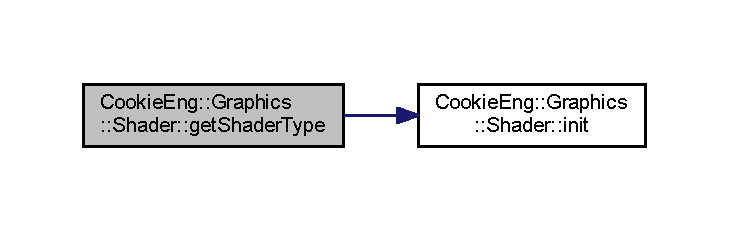
\includegraphics[width=350pt]{class_cookie_eng_1_1_graphics_1_1_shader_adde0294c86137d22a247bd011b8e40c8_cgraph}
\end{center}
\end{figure}
\mbox{\label{class_cookie_eng_1_1_graphics_1_1_shader_ae591a7107e04f835f1f8dbc42e0035c6}} 
\index{Cookie\+Eng\+::\+Graphics\+::\+Shader@{Cookie\+Eng\+::\+Graphics\+::\+Shader}!init@{init}}
\index{init@{init}!Cookie\+Eng\+::\+Graphics\+::\+Shader@{Cookie\+Eng\+::\+Graphics\+::\+Shader}}
\subsubsection{init()}
{\footnotesize\ttfamily void Cookie\+Eng\+::\+Graphics\+::\+Shader\+::init (\begin{DoxyParamCaption}{ }\end{DoxyParamCaption})\hspace{0.3cm}{\ttfamily [protected]}}



Initialises the \doxyref{Shader}{p.}{class_cookie_eng_1_1_graphics_1_1_shader}. 

Creates the shader on the G\+PU. This is seperated from the Constructor as initialising there was causing issues. \mbox{\label{class_cookie_eng_1_1_graphics_1_1_shader_aa11548ffaa72d77521576044a122af43}} 
\index{Cookie\+Eng\+::\+Graphics\+::\+Shader@{Cookie\+Eng\+::\+Graphics\+::\+Shader}!load@{load}}
\index{load@{load}!Cookie\+Eng\+::\+Graphics\+::\+Shader@{Cookie\+Eng\+::\+Graphics\+::\+Shader}}
\subsubsection{load()}
{\footnotesize\ttfamily bool Cookie\+Eng\+::\+Graphics\+::\+Shader\+::load (\begin{DoxyParamCaption}\item[{std\+::string}]{\+\_\+filepath }\end{DoxyParamCaption})}



Loads a text file into the \doxyref{Shader}{p.}{class_cookie_eng_1_1_graphics_1_1_shader}. 


\begin{DoxyParams}{Parameters}
{\em \+\_\+filepath} & The path to the Text File to be loaded \\
\hline
\end{DoxyParams}
\begin{DoxyReturn}{Returns}
the result of the load. True for sucessful, false for error.
\end{DoxyReturn}
Uses the file manager service to load a text file and places it onto the G\+PU. The shader is then verified to ensure the shader source is valid. \mbox{\label{class_cookie_eng_1_1_graphics_1_1_shader_a28abd2dba4a183cb810b196af2e1d5a3}} 
\index{Cookie\+Eng\+::\+Graphics\+::\+Shader@{Cookie\+Eng\+::\+Graphics\+::\+Shader}!verify@{verify}}
\index{verify@{verify}!Cookie\+Eng\+::\+Graphics\+::\+Shader@{Cookie\+Eng\+::\+Graphics\+::\+Shader}}
\subsubsection{verify()}
{\footnotesize\ttfamily bool Cookie\+Eng\+::\+Graphics\+::\+Shader\+::verify (\begin{DoxyParamCaption}{ }\end{DoxyParamCaption})}



Loads a text file into the \doxyref{Shader}{p.}{class_cookie_eng_1_1_graphics_1_1_shader}. 

\begin{DoxyReturn}{Returns}
The result of the verification. True for sucessful, false for error.
\end{DoxyReturn}
Verifies the shader complination and insures it will run. 

\subsection{Member Data Documentation}
\mbox{\label{class_cookie_eng_1_1_graphics_1_1_shader_a3c2b2bf0f97b9367c3871de99378bbbf}} 
\index{Cookie\+Eng\+::\+Graphics\+::\+Shader@{Cookie\+Eng\+::\+Graphics\+::\+Shader}!m\+\_\+shader\+ID@{m\+\_\+shader\+ID}}
\index{m\+\_\+shader\+ID@{m\+\_\+shader\+ID}!Cookie\+Eng\+::\+Graphics\+::\+Shader@{Cookie\+Eng\+::\+Graphics\+::\+Shader}}
\subsubsection{m\+\_\+shader\+ID}
{\footnotesize\ttfamily G\+Luint Cookie\+Eng\+::\+Graphics\+::\+Shader\+::m\+\_\+shader\+ID\hspace{0.3cm}{\ttfamily [protected]}}

The Open\+GL ID \mbox{\label{class_cookie_eng_1_1_graphics_1_1_shader_a50b512033ec7bd695dcd4daa2d971c22}} 
\index{Cookie\+Eng\+::\+Graphics\+::\+Shader@{Cookie\+Eng\+::\+Graphics\+::\+Shader}!m\+\_\+shader\+Type@{m\+\_\+shader\+Type}}
\index{m\+\_\+shader\+Type@{m\+\_\+shader\+Type}!Cookie\+Eng\+::\+Graphics\+::\+Shader@{Cookie\+Eng\+::\+Graphics\+::\+Shader}}
\subsubsection{m\+\_\+shader\+Type}
{\footnotesize\ttfamily Shader\+Type Cookie\+Eng\+::\+Graphics\+::\+Shader\+::m\+\_\+shader\+Type\hspace{0.3cm}{\ttfamily [protected]}}

The \doxyref{Shader}{p.}{class_cookie_eng_1_1_graphics_1_1_shader} Type \mbox{\label{class_cookie_eng_1_1_graphics_1_1_shader_acfa364395f90fdea34e5365221b3b564}} 
\index{Cookie\+Eng\+::\+Graphics\+::\+Shader@{Cookie\+Eng\+::\+Graphics\+::\+Shader}!m\+\_\+verified@{m\+\_\+verified}}
\index{m\+\_\+verified@{m\+\_\+verified}!Cookie\+Eng\+::\+Graphics\+::\+Shader@{Cookie\+Eng\+::\+Graphics\+::\+Shader}}
\subsubsection{m\+\_\+verified}
{\footnotesize\ttfamily bool Cookie\+Eng\+::\+Graphics\+::\+Shader\+::m\+\_\+verified\hspace{0.3cm}{\ttfamily [protected]}}

Flag to indiciate the verification state of the shader 

The documentation for this class was generated from the following file\+:\begin{DoxyCompactItemize}
\item 
include/Shader.\+h\end{DoxyCompactItemize}

\hypertarget{class_cookie_eng_1_1_resources_1_1_shader_program}{}\section{Cookie\+Eng\+:\+:Resources\+:\+:Shader\+Program Class Reference}
\label{class_cookie_eng_1_1_resources_1_1_shader_program}\index{Cookie\+Eng\+::\+Resources\+::\+Shader\+Program@{Cookie\+Eng\+::\+Resources\+::\+Shader\+Program}}


Abstracted Open\+GL Program.  




{\ttfamily \#include $<$Shader\+Program.\+h$>$}



Inherits \hyperlink{class_cookie_eng_1_1_resources_1_1_resource}{Cookie\+Eng\+::\+Resources\+::\+Resource}.

\subsection*{Public Member Functions}
\begin{DoxyCompactItemize}
\item 
\hyperlink{class_cookie_eng_1_1_resources_1_1_shader_program_a2de1a879247aa4ee38fc2c37408c5285}{Shader\+Program} ()
\begin{DoxyCompactList}\small\item\em Program Ctor. \end{DoxyCompactList}\item 
void \hyperlink{class_cookie_eng_1_1_resources_1_1_shader_program_aef29916bad667d1f820053fd891d9e58}{load} (const std\+::string \&\+\_\+name, const std\+::string \&\+\_\+filepath) override
\begin{DoxyCompactList}\small\item\em Loads the \hyperlink{class_cookie_eng_1_1_resources_1_1_shader_program}{Shader\+Program} from a file. \end{DoxyCompactList}\item 
\hyperlink{class_cookie_eng_1_1_resources_1_1_shader_program_a453b80b995d1b352c73fbac672d4dbc5}{$\sim$\+Shader\+Program} ()
\begin{DoxyCompactList}\small\item\em Program Ctor. \end{DoxyCompactList}\item 
void \hyperlink{class_cookie_eng_1_1_resources_1_1_shader_program_a951108feded567e573928dbb1d8caeca}{attach\+Shader} (\hyperlink{class_cookie_eng_1_1_graphics_1_1_shader}{Graphics\+::\+Shader} \&\+\_\+shader)
\begin{DoxyCompactList}\small\item\em Attaches a Shader to the Program. \end{DoxyCompactList}\item 
void \hyperlink{class_cookie_eng_1_1_resources_1_1_shader_program_ac1c103a1f174c4053a94b65e4f32ccfc}{link} ()
\begin{DoxyCompactList}\small\item\em Links the Shader Program. \end{DoxyCompactList}\item 
bool \hyperlink{class_cookie_eng_1_1_resources_1_1_shader_program_aaf510d906b80d93a10e90fa0fea26bb2}{verify} ()
\begin{DoxyCompactList}\small\item\em Verifys the Shader Program. \end{DoxyCompactList}\item 
void \hyperlink{class_cookie_eng_1_1_resources_1_1_shader_program_a4824333f2e0ee0e7cfc91cb0de92e065}{bind} () const
\begin{DoxyCompactList}\small\item\em Binds the shader. \end{DoxyCompactList}\item 
void \hyperlink{class_cookie_eng_1_1_resources_1_1_shader_program_a3fad7ebcee80d0cae25dfcca62c70e63}{un\+Bind} () const
\begin{DoxyCompactList}\small\item\em un\+Binds the shader \end{DoxyCompactList}\item 
int \hyperlink{class_cookie_eng_1_1_resources_1_1_shader_program_ae2fb823b3e8da3cf7154e0a8ffe25c85}{get\+Uniform\+Location} (const std\+::string \&\+\_\+name)
\begin{DoxyCompactList}\small\item\em Gets the location of the specified Uniform in a shader. \end{DoxyCompactList}\item 
void \hyperlink{class_cookie_eng_1_1_resources_1_1_shader_program_a6029828eaecc40f6a68779b86f5baf6d}{set\+Uniform1f} (const std\+::string \&\+\_\+name, float \+\_\+value)
\begin{DoxyCompactList}\small\item\em Sets a single float uniform. \end{DoxyCompactList}\item 
void \hyperlink{class_cookie_eng_1_1_resources_1_1_shader_program_ad13eabf4105d4d484d72c16696143254}{set\+Uniform3f} (const std\+::string \&\+\_\+name, float \+\_\+value1, float \+\_\+value2, float \+\_\+value3)
\begin{DoxyCompactList}\small\item\em Sets a vec3 uniform. \end{DoxyCompactList}\item 
void \hyperlink{class_cookie_eng_1_1_resources_1_1_shader_program_a7f584c7eb32c97424d2e08e0a0c90bef}{set\+Uniform4f} (const std\+::string \&\+\_\+name, float \+\_\+value1, float \+\_\+value2, float \+\_\+value3, float \+\_\+value4)
\begin{DoxyCompactList}\small\item\em Sets a vec4 uniform. \end{DoxyCompactList}\item 
void \hyperlink{class_cookie_eng_1_1_resources_1_1_shader_program_a328b09fef2d715e25f9dc3993b060b99}{set\+Uniform1i} (const std\+::string \&\+\_\+name, int \+\_\+value)
\begin{DoxyCompactList}\small\item\em Sets a single integar uniform. \end{DoxyCompactList}\item 
void \hyperlink{class_cookie_eng_1_1_resources_1_1_shader_program_a172752bb917cb141b1a3a1cc44b6a645}{set\+Uniform\+Mat4f} (const std\+::string \&\+\_\+name, const glm\+::mat4 \&\+\_\+value)
\begin{DoxyCompactList}\small\item\em Sets a matrix(4x4) uniform. \end{DoxyCompactList}\item 
void \hyperlink{class_cookie_eng_1_1_resources_1_1_shader_program_aea57a6a608fe57a1057d3a038bac16dd}{set\+Uniform\+Bool} (const std\+::string \&\+\_\+name, const bool \+\_\+value)
\begin{DoxyCompactList}\small\item\em Sets a boolean uniform. \end{DoxyCompactList}\end{DoxyCompactItemize}
\subsection*{Protected Attributes}
\begin{DoxyCompactItemize}
\item 
G\+Luint \hyperlink{class_cookie_eng_1_1_resources_1_1_shader_program_a78e4cd26f128e78c0949476a79ff1c45}{m\+\_\+program\+ID}
\item 
bool \hyperlink{class_cookie_eng_1_1_resources_1_1_shader_program_a826816da20d45149ac950ed64daeda50}{m\+\_\+verified}
\item 
std\+::unordered\+\_\+map$<$ std\+::string, int $>$ \hyperlink{class_cookie_eng_1_1_resources_1_1_shader_program_aba82e0d018c8086308c0cda41e268735}{m\+\_\+uniform\+Location\+Cache}
\end{DoxyCompactItemize}


\subsection{Detailed Description}
Abstracted Open\+GL Program. 

Abstracts and provides simple utilities for an Open\+GL Shader Program. The program M\+U\+ST be verified before it can be bound. 

\subsection{Constructor \& Destructor Documentation}
\mbox{\Hypertarget{class_cookie_eng_1_1_resources_1_1_shader_program_a2de1a879247aa4ee38fc2c37408c5285}\label{class_cookie_eng_1_1_resources_1_1_shader_program_a2de1a879247aa4ee38fc2c37408c5285}} 
\index{Cookie\+Eng\+::\+Resources\+::\+Shader\+Program@{Cookie\+Eng\+::\+Resources\+::\+Shader\+Program}!Shader\+Program@{Shader\+Program}}
\index{Shader\+Program@{Shader\+Program}!Cookie\+Eng\+::\+Resources\+::\+Shader\+Program@{Cookie\+Eng\+::\+Resources\+::\+Shader\+Program}}
\subsubsection{\texorpdfstring{Shader\+Program()}{ShaderProgram()}}
{\footnotesize\ttfamily Cookie\+Eng\+::\+Resources\+::\+Shader\+Program\+::\+Shader\+Program (\begin{DoxyParamCaption}{ }\end{DoxyParamCaption})}



Program Ctor. 

Creates a shader program and sets the verified status to false. \mbox{\Hypertarget{class_cookie_eng_1_1_resources_1_1_shader_program_a453b80b995d1b352c73fbac672d4dbc5}\label{class_cookie_eng_1_1_resources_1_1_shader_program_a453b80b995d1b352c73fbac672d4dbc5}} 
\index{Cookie\+Eng\+::\+Resources\+::\+Shader\+Program@{Cookie\+Eng\+::\+Resources\+::\+Shader\+Program}!````~Shader\+Program@{$\sim$\+Shader\+Program}}
\index{````~Shader\+Program@{$\sim$\+Shader\+Program}!Cookie\+Eng\+::\+Resources\+::\+Shader\+Program@{Cookie\+Eng\+::\+Resources\+::\+Shader\+Program}}
\subsubsection{\texorpdfstring{$\sim$\+Shader\+Program()}{~ShaderProgram()}}
{\footnotesize\ttfamily Cookie\+Eng\+::\+Resources\+::\+Shader\+Program\+::$\sim$\+Shader\+Program (\begin{DoxyParamCaption}{ }\end{DoxyParamCaption})\hspace{0.3cm}{\ttfamily [inline]}}



Program Ctor. 

Deletes the shader program and frees the G\+PU memory 

\subsection{Member Function Documentation}
\mbox{\Hypertarget{class_cookie_eng_1_1_resources_1_1_shader_program_a951108feded567e573928dbb1d8caeca}\label{class_cookie_eng_1_1_resources_1_1_shader_program_a951108feded567e573928dbb1d8caeca}} 
\index{Cookie\+Eng\+::\+Resources\+::\+Shader\+Program@{Cookie\+Eng\+::\+Resources\+::\+Shader\+Program}!attach\+Shader@{attach\+Shader}}
\index{attach\+Shader@{attach\+Shader}!Cookie\+Eng\+::\+Resources\+::\+Shader\+Program@{Cookie\+Eng\+::\+Resources\+::\+Shader\+Program}}
\subsubsection{\texorpdfstring{attach\+Shader()}{attachShader()}}
{\footnotesize\ttfamily void Cookie\+Eng\+::\+Resources\+::\+Shader\+Program\+::attach\+Shader (\begin{DoxyParamCaption}\item[{\hyperlink{class_cookie_eng_1_1_graphics_1_1_shader}{Graphics\+::\+Shader} \&}]{\+\_\+shader }\end{DoxyParamCaption})}



Attaches a Shader to the Program. 


\begin{DoxyParams}{Parameters}
{\em \+\_\+shader} & The shader to be attached\\
\hline
\end{DoxyParams}
Attaches a shader to the program. \mbox{\Hypertarget{class_cookie_eng_1_1_resources_1_1_shader_program_a4824333f2e0ee0e7cfc91cb0de92e065}\label{class_cookie_eng_1_1_resources_1_1_shader_program_a4824333f2e0ee0e7cfc91cb0de92e065}} 
\index{Cookie\+Eng\+::\+Resources\+::\+Shader\+Program@{Cookie\+Eng\+::\+Resources\+::\+Shader\+Program}!bind@{bind}}
\index{bind@{bind}!Cookie\+Eng\+::\+Resources\+::\+Shader\+Program@{Cookie\+Eng\+::\+Resources\+::\+Shader\+Program}}
\subsubsection{\texorpdfstring{bind()}{bind()}}
{\footnotesize\ttfamily void Cookie\+Eng\+::\+Resources\+::\+Shader\+Program\+::bind (\begin{DoxyParamCaption}{ }\end{DoxyParamCaption}) const}



Binds the shader. 

Binds the shader. For this to sucseed, the shader must be verified. \mbox{\Hypertarget{class_cookie_eng_1_1_resources_1_1_shader_program_ae2fb823b3e8da3cf7154e0a8ffe25c85}\label{class_cookie_eng_1_1_resources_1_1_shader_program_ae2fb823b3e8da3cf7154e0a8ffe25c85}} 
\index{Cookie\+Eng\+::\+Resources\+::\+Shader\+Program@{Cookie\+Eng\+::\+Resources\+::\+Shader\+Program}!get\+Uniform\+Location@{get\+Uniform\+Location}}
\index{get\+Uniform\+Location@{get\+Uniform\+Location}!Cookie\+Eng\+::\+Resources\+::\+Shader\+Program@{Cookie\+Eng\+::\+Resources\+::\+Shader\+Program}}
\subsubsection{\texorpdfstring{get\+Uniform\+Location()}{getUniformLocation()}}
{\footnotesize\ttfamily int Cookie\+Eng\+::\+Resources\+::\+Shader\+Program\+::get\+Uniform\+Location (\begin{DoxyParamCaption}\item[{const std\+::string \&}]{\+\_\+name }\end{DoxyParamCaption})}



Gets the location of the specified Uniform in a shader. 


\begin{DoxyParams}{Parameters}
{\em \+\_\+name} & The uniform to retrive \\
\hline
\end{DoxyParams}
\begin{DoxyReturn}{Returns}
The uniform location
\end{DoxyReturn}
Gets the location of a uniform in a shader based on its name. If the shader uniform location has not been requested before, it is cached so that future requests do not incur an Open\+GL call. \mbox{\Hypertarget{class_cookie_eng_1_1_resources_1_1_shader_program_ac1c103a1f174c4053a94b65e4f32ccfc}\label{class_cookie_eng_1_1_resources_1_1_shader_program_ac1c103a1f174c4053a94b65e4f32ccfc}} 
\index{Cookie\+Eng\+::\+Resources\+::\+Shader\+Program@{Cookie\+Eng\+::\+Resources\+::\+Shader\+Program}!link@{link}}
\index{link@{link}!Cookie\+Eng\+::\+Resources\+::\+Shader\+Program@{Cookie\+Eng\+::\+Resources\+::\+Shader\+Program}}
\subsubsection{\texorpdfstring{link()}{link()}}
{\footnotesize\ttfamily void Cookie\+Eng\+::\+Resources\+::\+Shader\+Program\+::link (\begin{DoxyParamCaption}{ }\end{DoxyParamCaption})}



Links the Shader Program. 

Links the shader program. \mbox{\Hypertarget{class_cookie_eng_1_1_resources_1_1_shader_program_aef29916bad667d1f820053fd891d9e58}\label{class_cookie_eng_1_1_resources_1_1_shader_program_aef29916bad667d1f820053fd891d9e58}} 
\index{Cookie\+Eng\+::\+Resources\+::\+Shader\+Program@{Cookie\+Eng\+::\+Resources\+::\+Shader\+Program}!load@{load}}
\index{load@{load}!Cookie\+Eng\+::\+Resources\+::\+Shader\+Program@{Cookie\+Eng\+::\+Resources\+::\+Shader\+Program}}
\subsubsection{\texorpdfstring{load()}{load()}}
{\footnotesize\ttfamily void Cookie\+Eng\+::\+Resources\+::\+Shader\+Program\+::load (\begin{DoxyParamCaption}\item[{const std\+::string \&}]{\+\_\+name,  }\item[{const std\+::string \&}]{\+\_\+filepath }\end{DoxyParamCaption})\hspace{0.3cm}{\ttfamily [override]}, {\ttfamily [virtual]}}



Loads the \hyperlink{class_cookie_eng_1_1_resources_1_1_shader_program}{Shader\+Program} from a file. 


\begin{DoxyParams}{Parameters}
{\em \+\_\+name} & The name to assign the shader \\
\hline
{\em \+\_\+filepath} & The filepath to load from\\
\hline
\end{DoxyParams}
Overrides the \hyperlink{class_cookie_eng_1_1_resources_1_1_resource}{Resource} load to allow loading from a .cng\+Shader file 

Reimplemented from \hyperlink{class_cookie_eng_1_1_resources_1_1_resource_a75648b8f2e442bebc90d6eb4ea3a2f6e}{Cookie\+Eng\+::\+Resources\+::\+Resource}.

\mbox{\Hypertarget{class_cookie_eng_1_1_resources_1_1_shader_program_a6029828eaecc40f6a68779b86f5baf6d}\label{class_cookie_eng_1_1_resources_1_1_shader_program_a6029828eaecc40f6a68779b86f5baf6d}} 
\index{Cookie\+Eng\+::\+Resources\+::\+Shader\+Program@{Cookie\+Eng\+::\+Resources\+::\+Shader\+Program}!set\+Uniform1f@{set\+Uniform1f}}
\index{set\+Uniform1f@{set\+Uniform1f}!Cookie\+Eng\+::\+Resources\+::\+Shader\+Program@{Cookie\+Eng\+::\+Resources\+::\+Shader\+Program}}
\subsubsection{\texorpdfstring{set\+Uniform1f()}{setUniform1f()}}
{\footnotesize\ttfamily void Cookie\+Eng\+::\+Resources\+::\+Shader\+Program\+::set\+Uniform1f (\begin{DoxyParamCaption}\item[{const std\+::string \&}]{\+\_\+name,  }\item[{float}]{\+\_\+value }\end{DoxyParamCaption})}



Sets a single float uniform. 


\begin{DoxyParams}{Parameters}
{\em \+\_\+name} & The name of the uniform to modify \\
\hline
{\em \+\_\+value} & The value to set the uniform to\\
\hline
\end{DoxyParams}
Uses the get\+Uniform\+Location method to get the uniform location and set it to the given value. \mbox{\Hypertarget{class_cookie_eng_1_1_resources_1_1_shader_program_a328b09fef2d715e25f9dc3993b060b99}\label{class_cookie_eng_1_1_resources_1_1_shader_program_a328b09fef2d715e25f9dc3993b060b99}} 
\index{Cookie\+Eng\+::\+Resources\+::\+Shader\+Program@{Cookie\+Eng\+::\+Resources\+::\+Shader\+Program}!set\+Uniform1i@{set\+Uniform1i}}
\index{set\+Uniform1i@{set\+Uniform1i}!Cookie\+Eng\+::\+Resources\+::\+Shader\+Program@{Cookie\+Eng\+::\+Resources\+::\+Shader\+Program}}
\subsubsection{\texorpdfstring{set\+Uniform1i()}{setUniform1i()}}
{\footnotesize\ttfamily void Cookie\+Eng\+::\+Resources\+::\+Shader\+Program\+::set\+Uniform1i (\begin{DoxyParamCaption}\item[{const std\+::string \&}]{\+\_\+name,  }\item[{int}]{\+\_\+value }\end{DoxyParamCaption})}



Sets a single integar uniform. 


\begin{DoxyParams}{Parameters}
{\em \+\_\+name} & The name of the uniform to modify \\
\hline
{\em \+\_\+value} & The value to set the uniform to\\
\hline
\end{DoxyParams}
Uses the get\+Uniform\+Location method to get the uniform location and set it to the given value. \mbox{\Hypertarget{class_cookie_eng_1_1_resources_1_1_shader_program_ad13eabf4105d4d484d72c16696143254}\label{class_cookie_eng_1_1_resources_1_1_shader_program_ad13eabf4105d4d484d72c16696143254}} 
\index{Cookie\+Eng\+::\+Resources\+::\+Shader\+Program@{Cookie\+Eng\+::\+Resources\+::\+Shader\+Program}!set\+Uniform3f@{set\+Uniform3f}}
\index{set\+Uniform3f@{set\+Uniform3f}!Cookie\+Eng\+::\+Resources\+::\+Shader\+Program@{Cookie\+Eng\+::\+Resources\+::\+Shader\+Program}}
\subsubsection{\texorpdfstring{set\+Uniform3f()}{setUniform3f()}}
{\footnotesize\ttfamily void Cookie\+Eng\+::\+Resources\+::\+Shader\+Program\+::set\+Uniform3f (\begin{DoxyParamCaption}\item[{const std\+::string \&}]{\+\_\+name,  }\item[{float}]{\+\_\+value1,  }\item[{float}]{\+\_\+value2,  }\item[{float}]{\+\_\+value3 }\end{DoxyParamCaption})}



Sets a vec3 uniform. 


\begin{DoxyParams}{Parameters}
{\em \+\_\+name} & The name of the uniform to modify \\
\hline
{\em \+\_\+value1} & The x value of the Vec4 \\
\hline
{\em \+\_\+value2} & The y value of the Vec4 \\
\hline
{\em \+\_\+value3} & The z value of the Vec4\\
\hline
\end{DoxyParams}
Uses the get\+Uniform\+Location method to get the uniform location and set it to the given values. \mbox{\Hypertarget{class_cookie_eng_1_1_resources_1_1_shader_program_a7f584c7eb32c97424d2e08e0a0c90bef}\label{class_cookie_eng_1_1_resources_1_1_shader_program_a7f584c7eb32c97424d2e08e0a0c90bef}} 
\index{Cookie\+Eng\+::\+Resources\+::\+Shader\+Program@{Cookie\+Eng\+::\+Resources\+::\+Shader\+Program}!set\+Uniform4f@{set\+Uniform4f}}
\index{set\+Uniform4f@{set\+Uniform4f}!Cookie\+Eng\+::\+Resources\+::\+Shader\+Program@{Cookie\+Eng\+::\+Resources\+::\+Shader\+Program}}
\subsubsection{\texorpdfstring{set\+Uniform4f()}{setUniform4f()}}
{\footnotesize\ttfamily void Cookie\+Eng\+::\+Resources\+::\+Shader\+Program\+::set\+Uniform4f (\begin{DoxyParamCaption}\item[{const std\+::string \&}]{\+\_\+name,  }\item[{float}]{\+\_\+value1,  }\item[{float}]{\+\_\+value2,  }\item[{float}]{\+\_\+value3,  }\item[{float}]{\+\_\+value4 }\end{DoxyParamCaption})}



Sets a vec4 uniform. 


\begin{DoxyParams}{Parameters}
{\em \+\_\+name} & The name of the uniform to modify \\
\hline
{\em \+\_\+value1} & The x value of the Vec4 \\
\hline
{\em \+\_\+value2} & The y value of the Vec4 \\
\hline
{\em \+\_\+value3} & The z value of the Vec4 \\
\hline
{\em \+\_\+value4} & The w value of the Vec4\\
\hline
\end{DoxyParams}
Uses the get\+Uniform\+Location method to get the uniform location and set it to the given values. \mbox{\Hypertarget{class_cookie_eng_1_1_resources_1_1_shader_program_aea57a6a608fe57a1057d3a038bac16dd}\label{class_cookie_eng_1_1_resources_1_1_shader_program_aea57a6a608fe57a1057d3a038bac16dd}} 
\index{Cookie\+Eng\+::\+Resources\+::\+Shader\+Program@{Cookie\+Eng\+::\+Resources\+::\+Shader\+Program}!set\+Uniform\+Bool@{set\+Uniform\+Bool}}
\index{set\+Uniform\+Bool@{set\+Uniform\+Bool}!Cookie\+Eng\+::\+Resources\+::\+Shader\+Program@{Cookie\+Eng\+::\+Resources\+::\+Shader\+Program}}
\subsubsection{\texorpdfstring{set\+Uniform\+Bool()}{setUniformBool()}}
{\footnotesize\ttfamily void Cookie\+Eng\+::\+Resources\+::\+Shader\+Program\+::set\+Uniform\+Bool (\begin{DoxyParamCaption}\item[{const std\+::string \&}]{\+\_\+name,  }\item[{const bool}]{\+\_\+value }\end{DoxyParamCaption})}



Sets a boolean uniform. 


\begin{DoxyParams}{Parameters}
{\em \+\_\+name} & The name of the uniform to modify \\
\hline
{\em \+\_\+value} & The value to set the uniform to\\
\hline
\end{DoxyParams}
Uses the get\+Uniform\+Location method to get the uniform location and set it to the given value. \mbox{\Hypertarget{class_cookie_eng_1_1_resources_1_1_shader_program_a172752bb917cb141b1a3a1cc44b6a645}\label{class_cookie_eng_1_1_resources_1_1_shader_program_a172752bb917cb141b1a3a1cc44b6a645}} 
\index{Cookie\+Eng\+::\+Resources\+::\+Shader\+Program@{Cookie\+Eng\+::\+Resources\+::\+Shader\+Program}!set\+Uniform\+Mat4f@{set\+Uniform\+Mat4f}}
\index{set\+Uniform\+Mat4f@{set\+Uniform\+Mat4f}!Cookie\+Eng\+::\+Resources\+::\+Shader\+Program@{Cookie\+Eng\+::\+Resources\+::\+Shader\+Program}}
\subsubsection{\texorpdfstring{set\+Uniform\+Mat4f()}{setUniformMat4f()}}
{\footnotesize\ttfamily void Cookie\+Eng\+::\+Resources\+::\+Shader\+Program\+::set\+Uniform\+Mat4f (\begin{DoxyParamCaption}\item[{const std\+::string \&}]{\+\_\+name,  }\item[{const glm\+::mat4 \&}]{\+\_\+value }\end{DoxyParamCaption})}



Sets a matrix(4x4) uniform. 


\begin{DoxyParams}{Parameters}
{\em \+\_\+name} & The name of the uniform to modify \\
\hline
{\em \+\_\+value} & The value to set the uniform to\\
\hline
\end{DoxyParams}
Uses the get\+Uniform\+Location method to get the uniform location and set it to the given value. \mbox{\Hypertarget{class_cookie_eng_1_1_resources_1_1_shader_program_a3fad7ebcee80d0cae25dfcca62c70e63}\label{class_cookie_eng_1_1_resources_1_1_shader_program_a3fad7ebcee80d0cae25dfcca62c70e63}} 
\index{Cookie\+Eng\+::\+Resources\+::\+Shader\+Program@{Cookie\+Eng\+::\+Resources\+::\+Shader\+Program}!un\+Bind@{un\+Bind}}
\index{un\+Bind@{un\+Bind}!Cookie\+Eng\+::\+Resources\+::\+Shader\+Program@{Cookie\+Eng\+::\+Resources\+::\+Shader\+Program}}
\subsubsection{\texorpdfstring{un\+Bind()}{unBind()}}
{\footnotesize\ttfamily void Cookie\+Eng\+::\+Resources\+::\+Shader\+Program\+::un\+Bind (\begin{DoxyParamCaption}{ }\end{DoxyParamCaption}) const}



un\+Binds the shader 

un\+Binds the shader. \mbox{\Hypertarget{class_cookie_eng_1_1_resources_1_1_shader_program_aaf510d906b80d93a10e90fa0fea26bb2}\label{class_cookie_eng_1_1_resources_1_1_shader_program_aaf510d906b80d93a10e90fa0fea26bb2}} 
\index{Cookie\+Eng\+::\+Resources\+::\+Shader\+Program@{Cookie\+Eng\+::\+Resources\+::\+Shader\+Program}!verify@{verify}}
\index{verify@{verify}!Cookie\+Eng\+::\+Resources\+::\+Shader\+Program@{Cookie\+Eng\+::\+Resources\+::\+Shader\+Program}}
\subsubsection{\texorpdfstring{verify()}{verify()}}
{\footnotesize\ttfamily bool Cookie\+Eng\+::\+Resources\+::\+Shader\+Program\+::verify (\begin{DoxyParamCaption}{ }\end{DoxyParamCaption})}



Verifys the Shader Program. 

Verifies the shader program and ensures it can run. 

\subsection{Member Data Documentation}
\mbox{\Hypertarget{class_cookie_eng_1_1_resources_1_1_shader_program_a78e4cd26f128e78c0949476a79ff1c45}\label{class_cookie_eng_1_1_resources_1_1_shader_program_a78e4cd26f128e78c0949476a79ff1c45}} 
\index{Cookie\+Eng\+::\+Resources\+::\+Shader\+Program@{Cookie\+Eng\+::\+Resources\+::\+Shader\+Program}!m\+\_\+program\+ID@{m\+\_\+program\+ID}}
\index{m\+\_\+program\+ID@{m\+\_\+program\+ID}!Cookie\+Eng\+::\+Resources\+::\+Shader\+Program@{Cookie\+Eng\+::\+Resources\+::\+Shader\+Program}}
\subsubsection{\texorpdfstring{m\+\_\+program\+ID}{m\_programID}}
{\footnotesize\ttfamily G\+Luint Cookie\+Eng\+::\+Resources\+::\+Shader\+Program\+::m\+\_\+program\+ID\hspace{0.3cm}{\ttfamily [protected]}}

The Open\+GL ID \mbox{\Hypertarget{class_cookie_eng_1_1_resources_1_1_shader_program_aba82e0d018c8086308c0cda41e268735}\label{class_cookie_eng_1_1_resources_1_1_shader_program_aba82e0d018c8086308c0cda41e268735}} 
\index{Cookie\+Eng\+::\+Resources\+::\+Shader\+Program@{Cookie\+Eng\+::\+Resources\+::\+Shader\+Program}!m\+\_\+uniform\+Location\+Cache@{m\+\_\+uniform\+Location\+Cache}}
\index{m\+\_\+uniform\+Location\+Cache@{m\+\_\+uniform\+Location\+Cache}!Cookie\+Eng\+::\+Resources\+::\+Shader\+Program@{Cookie\+Eng\+::\+Resources\+::\+Shader\+Program}}
\subsubsection{\texorpdfstring{m\+\_\+uniform\+Location\+Cache}{m\_uniformLocationCache}}
{\footnotesize\ttfamily std\+::unordered\+\_\+map$<$std\+::string, int$>$ Cookie\+Eng\+::\+Resources\+::\+Shader\+Program\+::m\+\_\+uniform\+Location\+Cache\hspace{0.3cm}{\ttfamily [protected]}}

The cache of uniform names to locations \mbox{\Hypertarget{class_cookie_eng_1_1_resources_1_1_shader_program_a826816da20d45149ac950ed64daeda50}\label{class_cookie_eng_1_1_resources_1_1_shader_program_a826816da20d45149ac950ed64daeda50}} 
\index{Cookie\+Eng\+::\+Resources\+::\+Shader\+Program@{Cookie\+Eng\+::\+Resources\+::\+Shader\+Program}!m\+\_\+verified@{m\+\_\+verified}}
\index{m\+\_\+verified@{m\+\_\+verified}!Cookie\+Eng\+::\+Resources\+::\+Shader\+Program@{Cookie\+Eng\+::\+Resources\+::\+Shader\+Program}}
\subsubsection{\texorpdfstring{m\+\_\+verified}{m\_verified}}
{\footnotesize\ttfamily bool Cookie\+Eng\+::\+Resources\+::\+Shader\+Program\+::m\+\_\+verified\hspace{0.3cm}{\ttfamily [protected]}}

Flag for the shaders verified status 

The documentation for this class was generated from the following file\+:\begin{DoxyCompactItemize}
\item 
D\+:/\+Programming/\+Engine Development/\+Cookie\+Eng/\+Cookie\+Eng/include/Shader\+Program.\+h\end{DoxyCompactItemize}

\hypertarget{class_test_entity}{}\section{Test\+Entity Class Reference}
\label{class_test_entity}\index{Test\+Entity@{Test\+Entity}}
\subsection*{Public Member Functions}
\begin{DoxyCompactItemize}
\item 
\mbox{\Hypertarget{class_test_entity_a3b92d1c3a43cbd536b7ae817b2155c9c}\label{class_test_entity_a3b92d1c3a43cbd536b7ae817b2155c9c}} 
void {\bfseries print} ()
\end{DoxyCompactItemize}


The documentation for this class was generated from the following file\+:\begin{DoxyCompactItemize}
\item 
D\+:/\+Programming/\+Engine Development/\+Cookie\+Eng/\+Cookie\+Eng/include/Test\+Entity.\+h\end{DoxyCompactItemize}

\hypertarget{class_cookie_eng_1_1_resources_1_1_texture}{}\section{Cookie\+Eng\+:\+:Resources\+:\+:Texture Class Reference}
\label{class_cookie_eng_1_1_resources_1_1_texture}\index{Cookie\+Eng\+::\+Resources\+::\+Texture@{Cookie\+Eng\+::\+Resources\+::\+Texture}}


An abstraction of an Open\+GL \hyperlink{class_cookie_eng_1_1_resources_1_1_texture}{Texture}.  




{\ttfamily \#include $<$Texture.\+h$>$}



Inherits \hyperlink{class_cookie_eng_1_1_resources_1_1_resource}{Cookie\+Eng\+::\+Resources\+::\+Resource}.

\subsection*{Public Member Functions}
\begin{DoxyCompactItemize}
\item 
\hyperlink{class_cookie_eng_1_1_resources_1_1_texture_ae7d09944ac0d60a971de919b2fd7108d}{Texture} ()
\begin{DoxyCompactList}\small\item\em \hyperlink{class_cookie_eng_1_1_resources_1_1_texture}{Texture} Ctor. \end{DoxyCompactList}\item 
\hyperlink{class_cookie_eng_1_1_resources_1_1_texture_a8bcbd117b436060b0540c3c80dc88b54}{Texture} (const std\+::string \&\+\_\+name, const std\+::string \&\+\_\+filepath)
\begin{DoxyCompactList}\small\item\em \hyperlink{class_cookie_eng_1_1_resources_1_1_texture}{Texture} Ctor. \end{DoxyCompactList}\item 
\hyperlink{class_cookie_eng_1_1_resources_1_1_texture_ac5830da00fa12695714d1ed03d03a591}{$\sim$\+Texture} ()
\begin{DoxyCompactList}\small\item\em \hyperlink{class_cookie_eng_1_1_resources_1_1_texture}{Texture} Dtor. \end{DoxyCompactList}\item 
void \hyperlink{class_cookie_eng_1_1_resources_1_1_texture_a1f2d72c781dba6262ac5ca6e8898fc8d}{load} (const std\+::string \&\+\_\+name, const std\+::string \&\+\_\+filepath) override
\begin{DoxyCompactList}\small\item\em Load \hyperlink{class_cookie_eng_1_1_resources_1_1_texture}{Texture}. \end{DoxyCompactList}\item 
void \hyperlink{class_cookie_eng_1_1_resources_1_1_texture_a19f26d4ff9f73e05562e00532466f4df}{bind} (G\+Luint \+\_\+slot=0) const
\begin{DoxyCompactList}\small\item\em Binds the \hyperlink{class_cookie_eng_1_1_resources_1_1_texture}{Texture}. \end{DoxyCompactList}\item 
void \hyperlink{class_cookie_eng_1_1_resources_1_1_texture_a1af11a58e5dc08fa18baeba8cee62109}{un\+Bind} ()
\begin{DoxyCompactList}\small\item\em Uninds the \hyperlink{class_cookie_eng_1_1_resources_1_1_texture}{Texture}. \end{DoxyCompactList}\item 
int \hyperlink{class_cookie_eng_1_1_resources_1_1_texture_a8f7b83fbbd885d0380100975fe9f5831}{get\+Width} () const
\begin{DoxyCompactList}\small\item\em Gets the with of the texture. \end{DoxyCompactList}\item 
int \hyperlink{class_cookie_eng_1_1_resources_1_1_texture_ac030b164a876de42ad141e9aab422a1c}{get\+Height} () const
\begin{DoxyCompactList}\small\item\em Gets the with of the texture. \end{DoxyCompactList}\end{DoxyCompactItemize}
\subsection*{Protected Attributes}
\begin{DoxyCompactItemize}
\item 
G\+Luint \hyperlink{class_cookie_eng_1_1_resources_1_1_texture_af0b6161b941846749407ba504e68ef5a}{m\+\_\+texture\+ID}
\item 
std\+::string \hyperlink{class_cookie_eng_1_1_resources_1_1_texture_ae67553523fd6d4c29ec23ef180d18bd8}{m\+\_\+filepath}
\item 
unsigned char $\ast$ \hyperlink{class_cookie_eng_1_1_resources_1_1_texture_ab52f89f4a8a5dc91e2581e53857036bf}{m\+\_\+local\+Buffer}
\item 
\mbox{\Hypertarget{class_cookie_eng_1_1_resources_1_1_texture_ab7a7ce9f87006faa0e921084b0885ce8}\label{class_cookie_eng_1_1_resources_1_1_texture_ab7a7ce9f87006faa0e921084b0885ce8}} 
int {\bfseries m\+\_\+width}
\item 
\mbox{\Hypertarget{class_cookie_eng_1_1_resources_1_1_texture_a27412b3f96850a2fa4aabde00741cac5}\label{class_cookie_eng_1_1_resources_1_1_texture_a27412b3f96850a2fa4aabde00741cac5}} 
int {\bfseries m\+\_\+height}
\item 
int \hyperlink{class_cookie_eng_1_1_resources_1_1_texture_ac873fd6475f9059603f79e389089ad48}{m\+\_\+\+B\+PP}
\end{DoxyCompactItemize}


\subsection{Detailed Description}
An abstraction of an Open\+GL \hyperlink{class_cookie_eng_1_1_resources_1_1_texture}{Texture}. 

This class handles the loading (move this) and assignment of an Open\+GL texture. 

\subsection{Constructor \& Destructor Documentation}
\mbox{\Hypertarget{class_cookie_eng_1_1_resources_1_1_texture_ae7d09944ac0d60a971de919b2fd7108d}\label{class_cookie_eng_1_1_resources_1_1_texture_ae7d09944ac0d60a971de919b2fd7108d}} 
\index{Cookie\+Eng\+::\+Resources\+::\+Texture@{Cookie\+Eng\+::\+Resources\+::\+Texture}!Texture@{Texture}}
\index{Texture@{Texture}!Cookie\+Eng\+::\+Resources\+::\+Texture@{Cookie\+Eng\+::\+Resources\+::\+Texture}}
\subsubsection{\texorpdfstring{Texture()}{Texture()}\hspace{0.1cm}{\footnotesize\ttfamily [1/2]}}
{\footnotesize\ttfamily Cookie\+Eng\+::\+Resources\+::\+Texture\+::\+Texture (\begin{DoxyParamCaption}{ }\end{DoxyParamCaption})}



\hyperlink{class_cookie_eng_1_1_resources_1_1_texture}{Texture} Ctor. 

Loads an image file using stb\+\_\+image and loads it into Open\+GL \mbox{\Hypertarget{class_cookie_eng_1_1_resources_1_1_texture_a8bcbd117b436060b0540c3c80dc88b54}\label{class_cookie_eng_1_1_resources_1_1_texture_a8bcbd117b436060b0540c3c80dc88b54}} 
\index{Cookie\+Eng\+::\+Resources\+::\+Texture@{Cookie\+Eng\+::\+Resources\+::\+Texture}!Texture@{Texture}}
\index{Texture@{Texture}!Cookie\+Eng\+::\+Resources\+::\+Texture@{Cookie\+Eng\+::\+Resources\+::\+Texture}}
\subsubsection{\texorpdfstring{Texture()}{Texture()}\hspace{0.1cm}{\footnotesize\ttfamily [2/2]}}
{\footnotesize\ttfamily Cookie\+Eng\+::\+Resources\+::\+Texture\+::\+Texture (\begin{DoxyParamCaption}\item[{const std\+::string \&}]{\+\_\+name,  }\item[{const std\+::string \&}]{\+\_\+filepath }\end{DoxyParamCaption})}



\hyperlink{class_cookie_eng_1_1_resources_1_1_texture}{Texture} Ctor. 


\begin{DoxyParams}{Parameters}
{\em \+\_\+filepath} & The path to the image to be loaded\\
\hline
\end{DoxyParams}
Loads an image file using stb\+\_\+image and loads it into Open\+GL \mbox{\Hypertarget{class_cookie_eng_1_1_resources_1_1_texture_ac5830da00fa12695714d1ed03d03a591}\label{class_cookie_eng_1_1_resources_1_1_texture_ac5830da00fa12695714d1ed03d03a591}} 
\index{Cookie\+Eng\+::\+Resources\+::\+Texture@{Cookie\+Eng\+::\+Resources\+::\+Texture}!````~Texture@{$\sim$\+Texture}}
\index{````~Texture@{$\sim$\+Texture}!Cookie\+Eng\+::\+Resources\+::\+Texture@{Cookie\+Eng\+::\+Resources\+::\+Texture}}
\subsubsection{\texorpdfstring{$\sim$\+Texture()}{~Texture()}}
{\footnotesize\ttfamily Cookie\+Eng\+::\+Resources\+::\+Texture\+::$\sim$\+Texture (\begin{DoxyParamCaption}{ }\end{DoxyParamCaption})}



\hyperlink{class_cookie_eng_1_1_resources_1_1_texture}{Texture} Dtor. 

Frees the Open\+GL \hyperlink{class_cookie_eng_1_1_resources_1_1_texture}{Texture} 

\subsection{Member Function Documentation}
\mbox{\Hypertarget{class_cookie_eng_1_1_resources_1_1_texture_a19f26d4ff9f73e05562e00532466f4df}\label{class_cookie_eng_1_1_resources_1_1_texture_a19f26d4ff9f73e05562e00532466f4df}} 
\index{Cookie\+Eng\+::\+Resources\+::\+Texture@{Cookie\+Eng\+::\+Resources\+::\+Texture}!bind@{bind}}
\index{bind@{bind}!Cookie\+Eng\+::\+Resources\+::\+Texture@{Cookie\+Eng\+::\+Resources\+::\+Texture}}
\subsubsection{\texorpdfstring{bind()}{bind()}}
{\footnotesize\ttfamily void Cookie\+Eng\+::\+Resources\+::\+Texture\+::bind (\begin{DoxyParamCaption}\item[{G\+Luint}]{\+\_\+slot = {\ttfamily 0} }\end{DoxyParamCaption}) const}



Binds the \hyperlink{class_cookie_eng_1_1_resources_1_1_texture}{Texture}. 


\begin{DoxyParams}{Parameters}
{\em \+\_\+slot} & The texture slot to bind the texture to\\
\hline
\end{DoxyParams}
Binds the texture to a specific slot in the Open\+GL texture slot array \mbox{\Hypertarget{class_cookie_eng_1_1_resources_1_1_texture_ac030b164a876de42ad141e9aab422a1c}\label{class_cookie_eng_1_1_resources_1_1_texture_ac030b164a876de42ad141e9aab422a1c}} 
\index{Cookie\+Eng\+::\+Resources\+::\+Texture@{Cookie\+Eng\+::\+Resources\+::\+Texture}!get\+Height@{get\+Height}}
\index{get\+Height@{get\+Height}!Cookie\+Eng\+::\+Resources\+::\+Texture@{Cookie\+Eng\+::\+Resources\+::\+Texture}}
\subsubsection{\texorpdfstring{get\+Height()}{getHeight()}}
{\footnotesize\ttfamily int Cookie\+Eng\+::\+Resources\+::\+Texture\+::get\+Height (\begin{DoxyParamCaption}{ }\end{DoxyParamCaption}) const\hspace{0.3cm}{\ttfamily [inline]}}



Gets the with of the texture. 

\begin{DoxyReturn}{Returns}
The texture height
\end{DoxyReturn}
Gets the height of the texture \mbox{\Hypertarget{class_cookie_eng_1_1_resources_1_1_texture_a8f7b83fbbd885d0380100975fe9f5831}\label{class_cookie_eng_1_1_resources_1_1_texture_a8f7b83fbbd885d0380100975fe9f5831}} 
\index{Cookie\+Eng\+::\+Resources\+::\+Texture@{Cookie\+Eng\+::\+Resources\+::\+Texture}!get\+Width@{get\+Width}}
\index{get\+Width@{get\+Width}!Cookie\+Eng\+::\+Resources\+::\+Texture@{Cookie\+Eng\+::\+Resources\+::\+Texture}}
\subsubsection{\texorpdfstring{get\+Width()}{getWidth()}}
{\footnotesize\ttfamily int Cookie\+Eng\+::\+Resources\+::\+Texture\+::get\+Width (\begin{DoxyParamCaption}{ }\end{DoxyParamCaption}) const\hspace{0.3cm}{\ttfamily [inline]}}



Gets the with of the texture. 

\begin{DoxyReturn}{Returns}
The texture width
\end{DoxyReturn}
Gets the with of the texture \mbox{\Hypertarget{class_cookie_eng_1_1_resources_1_1_texture_a1f2d72c781dba6262ac5ca6e8898fc8d}\label{class_cookie_eng_1_1_resources_1_1_texture_a1f2d72c781dba6262ac5ca6e8898fc8d}} 
\index{Cookie\+Eng\+::\+Resources\+::\+Texture@{Cookie\+Eng\+::\+Resources\+::\+Texture}!load@{load}}
\index{load@{load}!Cookie\+Eng\+::\+Resources\+::\+Texture@{Cookie\+Eng\+::\+Resources\+::\+Texture}}
\subsubsection{\texorpdfstring{load()}{load()}}
{\footnotesize\ttfamily void Cookie\+Eng\+::\+Resources\+::\+Texture\+::load (\begin{DoxyParamCaption}\item[{const std\+::string \&}]{\+\_\+name,  }\item[{const std\+::string \&}]{\+\_\+filepath }\end{DoxyParamCaption})\hspace{0.3cm}{\ttfamily [override]}, {\ttfamily [virtual]}}



Load \hyperlink{class_cookie_eng_1_1_resources_1_1_texture}{Texture}. 


\begin{DoxyParams}{Parameters}
{\em \+\_\+filepath} & The path to the image to be loaded\\
\hline
\end{DoxyParams}
Loads an image file using stb\+\_\+image and loads it into Open\+GL 

Reimplemented from \hyperlink{class_cookie_eng_1_1_resources_1_1_resource_a75648b8f2e442bebc90d6eb4ea3a2f6e}{Cookie\+Eng\+::\+Resources\+::\+Resource}.

\mbox{\Hypertarget{class_cookie_eng_1_1_resources_1_1_texture_a1af11a58e5dc08fa18baeba8cee62109}\label{class_cookie_eng_1_1_resources_1_1_texture_a1af11a58e5dc08fa18baeba8cee62109}} 
\index{Cookie\+Eng\+::\+Resources\+::\+Texture@{Cookie\+Eng\+::\+Resources\+::\+Texture}!un\+Bind@{un\+Bind}}
\index{un\+Bind@{un\+Bind}!Cookie\+Eng\+::\+Resources\+::\+Texture@{Cookie\+Eng\+::\+Resources\+::\+Texture}}
\subsubsection{\texorpdfstring{un\+Bind()}{unBind()}}
{\footnotesize\ttfamily void Cookie\+Eng\+::\+Resources\+::\+Texture\+::un\+Bind (\begin{DoxyParamCaption}{ }\end{DoxyParamCaption})\hspace{0.3cm}{\ttfamily [inline]}}



Uninds the \hyperlink{class_cookie_eng_1_1_resources_1_1_texture}{Texture}. 

Unbinds the texture. 

\subsection{Member Data Documentation}
\mbox{\Hypertarget{class_cookie_eng_1_1_resources_1_1_texture_ac873fd6475f9059603f79e389089ad48}\label{class_cookie_eng_1_1_resources_1_1_texture_ac873fd6475f9059603f79e389089ad48}} 
\index{Cookie\+Eng\+::\+Resources\+::\+Texture@{Cookie\+Eng\+::\+Resources\+::\+Texture}!m\+\_\+\+B\+PP@{m\+\_\+\+B\+PP}}
\index{m\+\_\+\+B\+PP@{m\+\_\+\+B\+PP}!Cookie\+Eng\+::\+Resources\+::\+Texture@{Cookie\+Eng\+::\+Resources\+::\+Texture}}
\subsubsection{\texorpdfstring{m\+\_\+\+B\+PP}{m\_BPP}}
{\footnotesize\ttfamily int Cookie\+Eng\+::\+Resources\+::\+Texture\+::m\+\_\+\+B\+PP\hspace{0.3cm}{\ttfamily [protected]}}

The width, height and bpp \mbox{\Hypertarget{class_cookie_eng_1_1_resources_1_1_texture_ae67553523fd6d4c29ec23ef180d18bd8}\label{class_cookie_eng_1_1_resources_1_1_texture_ae67553523fd6d4c29ec23ef180d18bd8}} 
\index{Cookie\+Eng\+::\+Resources\+::\+Texture@{Cookie\+Eng\+::\+Resources\+::\+Texture}!m\+\_\+filepath@{m\+\_\+filepath}}
\index{m\+\_\+filepath@{m\+\_\+filepath}!Cookie\+Eng\+::\+Resources\+::\+Texture@{Cookie\+Eng\+::\+Resources\+::\+Texture}}
\subsubsection{\texorpdfstring{m\+\_\+filepath}{m\_filepath}}
{\footnotesize\ttfamily std\+::string Cookie\+Eng\+::\+Resources\+::\+Texture\+::m\+\_\+filepath\hspace{0.3cm}{\ttfamily [protected]}}

The filepath to the texture \mbox{\Hypertarget{class_cookie_eng_1_1_resources_1_1_texture_ab52f89f4a8a5dc91e2581e53857036bf}\label{class_cookie_eng_1_1_resources_1_1_texture_ab52f89f4a8a5dc91e2581e53857036bf}} 
\index{Cookie\+Eng\+::\+Resources\+::\+Texture@{Cookie\+Eng\+::\+Resources\+::\+Texture}!m\+\_\+local\+Buffer@{m\+\_\+local\+Buffer}}
\index{m\+\_\+local\+Buffer@{m\+\_\+local\+Buffer}!Cookie\+Eng\+::\+Resources\+::\+Texture@{Cookie\+Eng\+::\+Resources\+::\+Texture}}
\subsubsection{\texorpdfstring{m\+\_\+local\+Buffer}{m\_localBuffer}}
{\footnotesize\ttfamily unsigned char$\ast$ Cookie\+Eng\+::\+Resources\+::\+Texture\+::m\+\_\+local\+Buffer\hspace{0.3cm}{\ttfamily [protected]}}

The local buffer for the loaded image \mbox{\Hypertarget{class_cookie_eng_1_1_resources_1_1_texture_af0b6161b941846749407ba504e68ef5a}\label{class_cookie_eng_1_1_resources_1_1_texture_af0b6161b941846749407ba504e68ef5a}} 
\index{Cookie\+Eng\+::\+Resources\+::\+Texture@{Cookie\+Eng\+::\+Resources\+::\+Texture}!m\+\_\+texture\+ID@{m\+\_\+texture\+ID}}
\index{m\+\_\+texture\+ID@{m\+\_\+texture\+ID}!Cookie\+Eng\+::\+Resources\+::\+Texture@{Cookie\+Eng\+::\+Resources\+::\+Texture}}
\subsubsection{\texorpdfstring{m\+\_\+texture\+ID}{m\_textureID}}
{\footnotesize\ttfamily G\+Luint Cookie\+Eng\+::\+Resources\+::\+Texture\+::m\+\_\+texture\+ID\hspace{0.3cm}{\ttfamily [protected]}}

The Open\+GL \hyperlink{class_cookie_eng_1_1_resources_1_1_texture}{Texture} ID 

The documentation for this class was generated from the following file\+:\begin{DoxyCompactItemize}
\item 
D\+:/\+Programming/\+Engine Development/\+Cookie\+Eng/\+Cookie\+Eng/include/Texture.\+h\end{DoxyCompactItemize}

\hypertarget{class_cookie_eng_1_1_threads_1_1_thread_pool}{}\section{Cookie\+Eng\+:\+:Threads\+:\+:Thread\+Pool Class Reference}
\label{class_cookie_eng_1_1_threads_1_1_thread_pool}\index{Cookie\+Eng\+::\+Threads\+::\+Thread\+Pool@{Cookie\+Eng\+::\+Threads\+::\+Thread\+Pool}}
\subsection*{Public Types}
\begin{DoxyCompactItemize}
\item 
\mbox{\Hypertarget{class_cookie_eng_1_1_threads_1_1_thread_pool_a3ec0c6482d6e8acd4bb3f49a976afbd4}\label{class_cookie_eng_1_1_threads_1_1_thread_pool_a3ec0c6482d6e8acd4bb3f49a976afbd4}} 
using {\bfseries Task} = std\+::function$<$ void()$>$
\end{DoxyCompactItemize}
\subsection*{Public Member Functions}
\begin{DoxyCompactItemize}
\item 
\mbox{\Hypertarget{class_cookie_eng_1_1_threads_1_1_thread_pool_a45d9e0c04c6ed38e994219591b62e775}\label{class_cookie_eng_1_1_threads_1_1_thread_pool_a45d9e0c04c6ed38e994219591b62e775}} 
{\bfseries Thread\+Pool} (const int \+\_\+num\+Threads)
\item 
\mbox{\Hypertarget{class_cookie_eng_1_1_threads_1_1_thread_pool_aa89bc838d587ed5c949a7b87a4f78c67}\label{class_cookie_eng_1_1_threads_1_1_thread_pool_aa89bc838d587ed5c949a7b87a4f78c67}} 
{\footnotesize template$<$class T $>$ }\\auto {\bfseries enqueue} (T \+\_\+task) -\/$>$ std\+::future$<$ decltype(\+\_\+task())$>$
\end{DoxyCompactItemize}
\subsection*{Protected Member Functions}
\begin{DoxyCompactItemize}
\item 
\mbox{\Hypertarget{class_cookie_eng_1_1_threads_1_1_thread_pool_aa1ec49665f4cef513dc11efd7bbf3ac6}\label{class_cookie_eng_1_1_threads_1_1_thread_pool_aa1ec49665f4cef513dc11efd7bbf3ac6}} 
void {\bfseries start} (const int \+\_\+num\+Threads)
\item 
\mbox{\Hypertarget{class_cookie_eng_1_1_threads_1_1_thread_pool_a2260d3d26f58843f9b87997aec916649}\label{class_cookie_eng_1_1_threads_1_1_thread_pool_a2260d3d26f58843f9b87997aec916649}} 
void {\bfseries stop} ()
\end{DoxyCompactItemize}
\subsection*{Protected Attributes}
\begin{DoxyCompactItemize}
\item 
\mbox{\Hypertarget{class_cookie_eng_1_1_threads_1_1_thread_pool_a4b2cc794349d82e9b75963d514eacdca}\label{class_cookie_eng_1_1_threads_1_1_thread_pool_a4b2cc794349d82e9b75963d514eacdca}} 
std\+::queue$<$ Task $>$ {\bfseries m\+\_\+tasks}
\item 
\mbox{\Hypertarget{class_cookie_eng_1_1_threads_1_1_thread_pool_ab8b101bddef80c83f481718a81a43945}\label{class_cookie_eng_1_1_threads_1_1_thread_pool_ab8b101bddef80c83f481718a81a43945}} 
std\+::vector$<$ std\+::thread $>$ {\bfseries m\+\_\+threads}
\item 
\mbox{\Hypertarget{class_cookie_eng_1_1_threads_1_1_thread_pool_a8aa7f0e105013ccb141031d5f11cd640}\label{class_cookie_eng_1_1_threads_1_1_thread_pool_a8aa7f0e105013ccb141031d5f11cd640}} 
std\+::condition\+\_\+variable {\bfseries m\+\_\+cond\+\_\+event}
\item 
\mbox{\Hypertarget{class_cookie_eng_1_1_threads_1_1_thread_pool_ac3206f1c04bd54fbac38134b105ec2b3}\label{class_cookie_eng_1_1_threads_1_1_thread_pool_ac3206f1c04bd54fbac38134b105ec2b3}} 
std\+::mutex {\bfseries m\+\_\+event\+Mutex}
\item 
\mbox{\Hypertarget{class_cookie_eng_1_1_threads_1_1_thread_pool_aee95f4d4dd35bb62b7bb1cf05bc8802b}\label{class_cookie_eng_1_1_threads_1_1_thread_pool_aee95f4d4dd35bb62b7bb1cf05bc8802b}} 
bool {\bfseries m\+\_\+stopping} = false
\end{DoxyCompactItemize}


The documentation for this class was generated from the following file\+:\begin{DoxyCompactItemize}
\item 
D\+:/\+Programming/\+Engine Development/\+Cookie\+Eng/\+Cookie\+Eng/include/Thread\+Pool.\+h\end{DoxyCompactItemize}

\hypertarget{struct_cookie_eng_1_1_utilities_1_1_times}{}\section{Cookie\+Eng\+:\+:Utilities\+:\+:Times Class Reference}
\label{struct_cookie_eng_1_1_utilities_1_1_times}\index{Cookie\+Eng\+::\+Utilities\+::\+Times@{Cookie\+Eng\+::\+Utilities\+::\+Times}}


Holds engine time values.  




{\ttfamily \#include $<$Times.\+h$>$}

\subsection*{Static Public Attributes}
\begin{DoxyCompactItemize}
\item 
static double \hyperlink{struct_cookie_eng_1_1_utilities_1_1_times_abab3889716480204f7250ff3347b8392}{delta\+Time}
\end{DoxyCompactItemize}


\subsection{Detailed Description}
Holds engine time values. 

Frame and engine timing such as Delta Time are stored in this for use all over the engine. This is usefull for frame independent movement etc. 

\subsection{Member Data Documentation}
\mbox{\Hypertarget{struct_cookie_eng_1_1_utilities_1_1_times_abab3889716480204f7250ff3347b8392}\label{struct_cookie_eng_1_1_utilities_1_1_times_abab3889716480204f7250ff3347b8392}} 
\index{Cookie\+Eng\+::\+Utilities\+::\+Times@{Cookie\+Eng\+::\+Utilities\+::\+Times}!delta\+Time@{delta\+Time}}
\index{delta\+Time@{delta\+Time}!Cookie\+Eng\+::\+Utilities\+::\+Times@{Cookie\+Eng\+::\+Utilities\+::\+Times}}
\subsubsection{\texorpdfstring{delta\+Time}{deltaTime}}
{\footnotesize\ttfamily double Cookie\+Eng\+::\+Utilities\+::\+Times\+::delta\+Time\hspace{0.3cm}{\ttfamily [static]}}

The time in seconds it took to complete the last frame 

The documentation for this class was generated from the following file\+:\begin{DoxyCompactItemize}
\item 
D\+:/\+Programming/\+Engine Development/\+Cookie\+Eng/\+Cookie\+Eng/include/Times.\+h\end{DoxyCompactItemize}

\hypertarget{class_cookie_eng_1_1_components_1_1_transform}{}\section{Cookie\+Eng\+:\+:Components\+:\+:Transform Class Reference}
\label{class_cookie_eng_1_1_components_1_1_transform}\index{Cookie\+Eng\+::\+Components\+::\+Transform@{Cookie\+Eng\+::\+Components\+::\+Transform}}


A \hyperlink{class_cookie_eng_1_1_components_1_1_transform}{Transform} Component.  




{\ttfamily \#include $<$Transform.\+h$>$}



Inherits \hyperlink{class_cookie_eng_1_1_e_c_s_1_1_component}{Cookie\+Eng\+::\+E\+C\+S\+::\+Component}.

\subsection*{Public Member Functions}
\begin{DoxyCompactItemize}
\item 
\hyperlink{class_cookie_eng_1_1_components_1_1_transform_a477bc2eb1d09fecdcb7399d5124ccd0d}{Transform} ()
\begin{DoxyCompactList}\small\item\em \hyperlink{class_cookie_eng_1_1_components_1_1_transform}{Transform} Ctor. \end{DoxyCompactList}\item 
\hyperlink{class_cookie_eng_1_1_components_1_1_transform_ad07b4e7f04ec0c60646339be8b67c69c}{$\sim$\+Transform} ()
\begin{DoxyCompactList}\small\item\em \hyperlink{class_cookie_eng_1_1_components_1_1_transform}{Transform} Dtor. \end{DoxyCompactList}\item 
void \hyperlink{class_cookie_eng_1_1_components_1_1_transform_a169960289f66442f692bb52c4c86478e}{set\+Model\+Matrix} ()
\begin{DoxyCompactList}\small\item\em Sets the Model Matrix. \end{DoxyCompactList}\item 
glm\+::mat4 \hyperlink{class_cookie_eng_1_1_components_1_1_transform_a0d18917e8701c84b6759823f785969de}{get\+Matrix} ()
\begin{DoxyCompactList}\small\item\em Gets the model matrix. \end{DoxyCompactList}\item 
glm\+::vec3 \hyperlink{class_cookie_eng_1_1_components_1_1_transform_a20c33650a735e8c9c54b232e871ff526}{get\+Position\+Vec3} ()
\begin{DoxyCompactList}\small\item\em Gets the Position. \end{DoxyCompactList}\item 
void \hyperlink{class_cookie_eng_1_1_components_1_1_transform_ac20843bb62dfdf7fce9fa96368b5a807}{set\+Position} (const glm\+::vec3 \&\+\_\+position)
\begin{DoxyCompactList}\small\item\em Sets the absolute position. \end{DoxyCompactList}\item 
void \hyperlink{class_cookie_eng_1_1_components_1_1_transform_afe2e00e8126fd92eab8c2e1a5725b2c5}{translate} (const glm\+::vec3 \&\+\_\+position)
\begin{DoxyCompactList}\small\item\em Moves the transform to a new position relative to its old position. \end{DoxyCompactList}\item 
void \hyperlink{class_cookie_eng_1_1_components_1_1_transform_a382a16d437c34d7e345a60d11a9578b2}{set\+Rotation} (const float \+\_\+rotation, const glm\+::vec3 \&\+\_\+axis)
\begin{DoxyCompactList}\small\item\em Sets the absolute rotation. \end{DoxyCompactList}\item 
void \hyperlink{class_cookie_eng_1_1_components_1_1_transform_a061b3b2b5d33c1dda2955e9b2e01d736}{rotate} (const float \+\_\+rotation, const glm\+::vec3 \+\_\+axis)
\begin{DoxyCompactList}\small\item\em Rotates the transform to a new rotation relative to its old rotation. \end{DoxyCompactList}\item 
glm\+::mat4 \hyperlink{class_cookie_eng_1_1_components_1_1_transform_a069b3948eab396b9f83fa9b983983e09}{get\+Rotation\+Matrix} ()
\begin{DoxyCompactList}\small\item\em Getter for the rotation matrix. \end{DoxyCompactList}\item 
glm\+::vec3 \hyperlink{class_cookie_eng_1_1_components_1_1_transform_a8ed85d55bd1084dde196ceb1b16fa736}{get\+Scale\+Vec3} ()
\begin{DoxyCompactList}\small\item\em Gets the Position. \end{DoxyCompactList}\item 
void \hyperlink{class_cookie_eng_1_1_components_1_1_transform_a6dadfac773418cc71d538c89219af0db}{set\+Scale} (const glm\+::vec3 \&\+\_\+scale)
\begin{DoxyCompactList}\small\item\em Sets the absolute position. \end{DoxyCompactList}\item 
void \hyperlink{class_cookie_eng_1_1_components_1_1_transform_abfb2568bd0222d8687593d253688f99f}{scale} (const glm\+::vec3 \&\+\_\+scale)
\begin{DoxyCompactList}\small\item\em Moves the transform to a new position relative to its old position. \end{DoxyCompactList}\end{DoxyCompactItemize}
\subsection*{Protected Attributes}
\begin{DoxyCompactItemize}
\item 
glm\+::vec3 \hyperlink{class_cookie_eng_1_1_components_1_1_transform_a6e99757f68b1de46b9caeaacdf6e88ae}{m\+\_\+position}
\item 
glm\+::vec3 \hyperlink{class_cookie_eng_1_1_components_1_1_transform_ab47df9535ea8c9b95ebd86b16381b86b}{m\+\_\+rotation}
\item 
glm\+::vec3 \hyperlink{class_cookie_eng_1_1_components_1_1_transform_a0bac06b21d49e96337fc82910fb4a5e9}{m\+\_\+scale}
\item 
glm\+::mat4 \hyperlink{class_cookie_eng_1_1_components_1_1_transform_ab4c66323537c12117739471665c6ddf9}{m\+\_\+model\+Matrix}
\item 
glm\+::mat4 \hyperlink{class_cookie_eng_1_1_components_1_1_transform_a247892c3be676ab7ec613600435cead8}{m\+\_\+model\+Matrix\+NS}
\item 
glm\+::mat4 \hyperlink{class_cookie_eng_1_1_components_1_1_transform_a8ab2d1886012bb7942ef4e4aafbd0321}{m\+\_\+translation\+Matrix}
\item 
glm\+::mat4 \hyperlink{class_cookie_eng_1_1_components_1_1_transform_aea4ccabe5423b8d31df96c6b9bd5553e}{m\+\_\+rotation\+Matrix}
\item 
glm\+::mat4 \hyperlink{class_cookie_eng_1_1_components_1_1_transform_aa41354d093d9821fb9a790517d97732f}{m\+\_\+scale\+Matrix}
\end{DoxyCompactItemize}
\subsection*{Additional Inherited Members}


\subsection{Detailed Description}
A \hyperlink{class_cookie_eng_1_1_components_1_1_transform}{Transform} Component. 

Tracks a position / rotation and scale in 3D space using the G\+LM library 

\subsection{Constructor \& Destructor Documentation}
\mbox{\Hypertarget{class_cookie_eng_1_1_components_1_1_transform_a477bc2eb1d09fecdcb7399d5124ccd0d}\label{class_cookie_eng_1_1_components_1_1_transform_a477bc2eb1d09fecdcb7399d5124ccd0d}} 
\index{Cookie\+Eng\+::\+Components\+::\+Transform@{Cookie\+Eng\+::\+Components\+::\+Transform}!Transform@{Transform}}
\index{Transform@{Transform}!Cookie\+Eng\+::\+Components\+::\+Transform@{Cookie\+Eng\+::\+Components\+::\+Transform}}
\subsubsection{\texorpdfstring{Transform()}{Transform()}}
{\footnotesize\ttfamily Cookie\+Eng\+::\+Components\+::\+Transform\+::\+Transform (\begin{DoxyParamCaption}{ }\end{DoxyParamCaption})}



\hyperlink{class_cookie_eng_1_1_components_1_1_transform}{Transform} Ctor. 

Creates a transform at the world 0, 0, 0 with default rotation and scale \mbox{\Hypertarget{class_cookie_eng_1_1_components_1_1_transform_ad07b4e7f04ec0c60646339be8b67c69c}\label{class_cookie_eng_1_1_components_1_1_transform_ad07b4e7f04ec0c60646339be8b67c69c}} 
\index{Cookie\+Eng\+::\+Components\+::\+Transform@{Cookie\+Eng\+::\+Components\+::\+Transform}!````~Transform@{$\sim$\+Transform}}
\index{````~Transform@{$\sim$\+Transform}!Cookie\+Eng\+::\+Components\+::\+Transform@{Cookie\+Eng\+::\+Components\+::\+Transform}}
\subsubsection{\texorpdfstring{$\sim$\+Transform()}{~Transform()}}
{\footnotesize\ttfamily Cookie\+Eng\+::\+Components\+::\+Transform\+::$\sim$\+Transform (\begin{DoxyParamCaption}{ }\end{DoxyParamCaption})\hspace{0.3cm}{\ttfamily [inline]}}



\hyperlink{class_cookie_eng_1_1_components_1_1_transform}{Transform} Dtor. 

Deletes a transform 

\subsection{Member Function Documentation}
\mbox{\Hypertarget{class_cookie_eng_1_1_components_1_1_transform_a0d18917e8701c84b6759823f785969de}\label{class_cookie_eng_1_1_components_1_1_transform_a0d18917e8701c84b6759823f785969de}} 
\index{Cookie\+Eng\+::\+Components\+::\+Transform@{Cookie\+Eng\+::\+Components\+::\+Transform}!get\+Matrix@{get\+Matrix}}
\index{get\+Matrix@{get\+Matrix}!Cookie\+Eng\+::\+Components\+::\+Transform@{Cookie\+Eng\+::\+Components\+::\+Transform}}
\subsubsection{\texorpdfstring{get\+Matrix()}{getMatrix()}}
{\footnotesize\ttfamily glm\+::mat4 Cookie\+Eng\+::\+Components\+::\+Transform\+::get\+Matrix (\begin{DoxyParamCaption}{ }\end{DoxyParamCaption})\hspace{0.3cm}{\ttfamily [inline]}}



Gets the model matrix. 

\begin{DoxyReturn}{Returns}
The model matrix
\end{DoxyReturn}
Returns the model matrix of the transform \mbox{\Hypertarget{class_cookie_eng_1_1_components_1_1_transform_a20c33650a735e8c9c54b232e871ff526}\label{class_cookie_eng_1_1_components_1_1_transform_a20c33650a735e8c9c54b232e871ff526}} 
\index{Cookie\+Eng\+::\+Components\+::\+Transform@{Cookie\+Eng\+::\+Components\+::\+Transform}!get\+Position\+Vec3@{get\+Position\+Vec3}}
\index{get\+Position\+Vec3@{get\+Position\+Vec3}!Cookie\+Eng\+::\+Components\+::\+Transform@{Cookie\+Eng\+::\+Components\+::\+Transform}}
\subsubsection{\texorpdfstring{get\+Position\+Vec3()}{getPositionVec3()}}
{\footnotesize\ttfamily glm\+::vec3 Cookie\+Eng\+::\+Components\+::\+Transform\+::get\+Position\+Vec3 (\begin{DoxyParamCaption}{ }\end{DoxyParamCaption})\hspace{0.3cm}{\ttfamily [inline]}}



Gets the Position. 

\begin{DoxyReturn}{Returns}
The position vector in 3D
\end{DoxyReturn}
Returns the position vector \mbox{\Hypertarget{class_cookie_eng_1_1_components_1_1_transform_a069b3948eab396b9f83fa9b983983e09}\label{class_cookie_eng_1_1_components_1_1_transform_a069b3948eab396b9f83fa9b983983e09}} 
\index{Cookie\+Eng\+::\+Components\+::\+Transform@{Cookie\+Eng\+::\+Components\+::\+Transform}!get\+Rotation\+Matrix@{get\+Rotation\+Matrix}}
\index{get\+Rotation\+Matrix@{get\+Rotation\+Matrix}!Cookie\+Eng\+::\+Components\+::\+Transform@{Cookie\+Eng\+::\+Components\+::\+Transform}}
\subsubsection{\texorpdfstring{get\+Rotation\+Matrix()}{getRotationMatrix()}}
{\footnotesize\ttfamily glm\+::mat4 Cookie\+Eng\+::\+Components\+::\+Transform\+::get\+Rotation\+Matrix (\begin{DoxyParamCaption}{ }\end{DoxyParamCaption})\hspace{0.3cm}{\ttfamily [inline]}}



Getter for the rotation matrix. 

\begin{DoxyReturn}{Returns}
The rotation matrix of the transform
\end{DoxyReturn}
Gets the rotation matrix of the transform. Used by \hyperlink{class_cookie_eng_1_1_components_1_1_bounding_box}{Bounding\+Box}. \mbox{\Hypertarget{class_cookie_eng_1_1_components_1_1_transform_a8ed85d55bd1084dde196ceb1b16fa736}\label{class_cookie_eng_1_1_components_1_1_transform_a8ed85d55bd1084dde196ceb1b16fa736}} 
\index{Cookie\+Eng\+::\+Components\+::\+Transform@{Cookie\+Eng\+::\+Components\+::\+Transform}!get\+Scale\+Vec3@{get\+Scale\+Vec3}}
\index{get\+Scale\+Vec3@{get\+Scale\+Vec3}!Cookie\+Eng\+::\+Components\+::\+Transform@{Cookie\+Eng\+::\+Components\+::\+Transform}}
\subsubsection{\texorpdfstring{get\+Scale\+Vec3()}{getScaleVec3()}}
{\footnotesize\ttfamily glm\+::vec3 Cookie\+Eng\+::\+Components\+::\+Transform\+::get\+Scale\+Vec3 (\begin{DoxyParamCaption}{ }\end{DoxyParamCaption})\hspace{0.3cm}{\ttfamily [inline]}}



Gets the Position. 

\begin{DoxyReturn}{Returns}
The position vector in 3D
\end{DoxyReturn}
Returns the position vector \mbox{\Hypertarget{class_cookie_eng_1_1_components_1_1_transform_a061b3b2b5d33c1dda2955e9b2e01d736}\label{class_cookie_eng_1_1_components_1_1_transform_a061b3b2b5d33c1dda2955e9b2e01d736}} 
\index{Cookie\+Eng\+::\+Components\+::\+Transform@{Cookie\+Eng\+::\+Components\+::\+Transform}!rotate@{rotate}}
\index{rotate@{rotate}!Cookie\+Eng\+::\+Components\+::\+Transform@{Cookie\+Eng\+::\+Components\+::\+Transform}}
\subsubsection{\texorpdfstring{rotate()}{rotate()}}
{\footnotesize\ttfamily void Cookie\+Eng\+::\+Components\+::\+Transform\+::rotate (\begin{DoxyParamCaption}\item[{const float}]{\+\_\+rotation,  }\item[{const glm\+::vec3}]{\+\_\+axis }\end{DoxyParamCaption})}



Rotates the transform to a new rotation relative to its old rotation. 


\begin{DoxyParams}{Parameters}
{\em \+\_\+rotation} & The difference in rotation to apply \\
\hline
{\em \+\_\+axis} & The axis to rotate on\\
\hline
\end{DoxyParams}
Changes the rotation of the transform by the given vector 3D. \mbox{\Hypertarget{class_cookie_eng_1_1_components_1_1_transform_abfb2568bd0222d8687593d253688f99f}\label{class_cookie_eng_1_1_components_1_1_transform_abfb2568bd0222d8687593d253688f99f}} 
\index{Cookie\+Eng\+::\+Components\+::\+Transform@{Cookie\+Eng\+::\+Components\+::\+Transform}!scale@{scale}}
\index{scale@{scale}!Cookie\+Eng\+::\+Components\+::\+Transform@{Cookie\+Eng\+::\+Components\+::\+Transform}}
\subsubsection{\texorpdfstring{scale()}{scale()}}
{\footnotesize\ttfamily void Cookie\+Eng\+::\+Components\+::\+Transform\+::scale (\begin{DoxyParamCaption}\item[{const glm\+::vec3 \&}]{\+\_\+scale }\end{DoxyParamCaption})}



Moves the transform to a new position relative to its old position. 


\begin{DoxyParams}{Parameters}
{\em \+\_\+position} & The difference in position to apply\\
\hline
\end{DoxyParams}
Translates the position of the transform by the given vector 3D. \mbox{\Hypertarget{class_cookie_eng_1_1_components_1_1_transform_a169960289f66442f692bb52c4c86478e}\label{class_cookie_eng_1_1_components_1_1_transform_a169960289f66442f692bb52c4c86478e}} 
\index{Cookie\+Eng\+::\+Components\+::\+Transform@{Cookie\+Eng\+::\+Components\+::\+Transform}!set\+Model\+Matrix@{set\+Model\+Matrix}}
\index{set\+Model\+Matrix@{set\+Model\+Matrix}!Cookie\+Eng\+::\+Components\+::\+Transform@{Cookie\+Eng\+::\+Components\+::\+Transform}}
\subsubsection{\texorpdfstring{set\+Model\+Matrix()}{setModelMatrix()}}
{\footnotesize\ttfamily void Cookie\+Eng\+::\+Components\+::\+Transform\+::set\+Model\+Matrix (\begin{DoxyParamCaption}{ }\end{DoxyParamCaption})}



Sets the Model Matrix. 

Calculates the new Model Matrix from the internal Vec3 attributes \mbox{\Hypertarget{class_cookie_eng_1_1_components_1_1_transform_ac20843bb62dfdf7fce9fa96368b5a807}\label{class_cookie_eng_1_1_components_1_1_transform_ac20843bb62dfdf7fce9fa96368b5a807}} 
\index{Cookie\+Eng\+::\+Components\+::\+Transform@{Cookie\+Eng\+::\+Components\+::\+Transform}!set\+Position@{set\+Position}}
\index{set\+Position@{set\+Position}!Cookie\+Eng\+::\+Components\+::\+Transform@{Cookie\+Eng\+::\+Components\+::\+Transform}}
\subsubsection{\texorpdfstring{set\+Position()}{setPosition()}}
{\footnotesize\ttfamily void Cookie\+Eng\+::\+Components\+::\+Transform\+::set\+Position (\begin{DoxyParamCaption}\item[{const glm\+::vec3 \&}]{\+\_\+position }\end{DoxyParamCaption})}



Sets the absolute position. 


\begin{DoxyParams}{Parameters}
{\em \+\_\+position} & The new position\\
\hline
\end{DoxyParams}
Sets the new position of the transform, disregarding its old position \mbox{\Hypertarget{class_cookie_eng_1_1_components_1_1_transform_a382a16d437c34d7e345a60d11a9578b2}\label{class_cookie_eng_1_1_components_1_1_transform_a382a16d437c34d7e345a60d11a9578b2}} 
\index{Cookie\+Eng\+::\+Components\+::\+Transform@{Cookie\+Eng\+::\+Components\+::\+Transform}!set\+Rotation@{set\+Rotation}}
\index{set\+Rotation@{set\+Rotation}!Cookie\+Eng\+::\+Components\+::\+Transform@{Cookie\+Eng\+::\+Components\+::\+Transform}}
\subsubsection{\texorpdfstring{set\+Rotation()}{setRotation()}}
{\footnotesize\ttfamily void Cookie\+Eng\+::\+Components\+::\+Transform\+::set\+Rotation (\begin{DoxyParamCaption}\item[{const float}]{\+\_\+rotation,  }\item[{const glm\+::vec3 \&}]{\+\_\+axis }\end{DoxyParamCaption})}



Sets the absolute rotation. 


\begin{DoxyParams}{Parameters}
{\em \+\_\+rotation} & The new rotation \\
\hline
{\em \+\_\+axis} & The axis to rotate on\\
\hline
\end{DoxyParams}
Sets the new rotation of the transform, disregarding its old rotation \mbox{\Hypertarget{class_cookie_eng_1_1_components_1_1_transform_a6dadfac773418cc71d538c89219af0db}\label{class_cookie_eng_1_1_components_1_1_transform_a6dadfac773418cc71d538c89219af0db}} 
\index{Cookie\+Eng\+::\+Components\+::\+Transform@{Cookie\+Eng\+::\+Components\+::\+Transform}!set\+Scale@{set\+Scale}}
\index{set\+Scale@{set\+Scale}!Cookie\+Eng\+::\+Components\+::\+Transform@{Cookie\+Eng\+::\+Components\+::\+Transform}}
\subsubsection{\texorpdfstring{set\+Scale()}{setScale()}}
{\footnotesize\ttfamily void Cookie\+Eng\+::\+Components\+::\+Transform\+::set\+Scale (\begin{DoxyParamCaption}\item[{const glm\+::vec3 \&}]{\+\_\+scale }\end{DoxyParamCaption})}



Sets the absolute position. 


\begin{DoxyParams}{Parameters}
{\em \+\_\+position} & The new position\\
\hline
\end{DoxyParams}
Sets the new position of the transform, disregarding its old position \mbox{\Hypertarget{class_cookie_eng_1_1_components_1_1_transform_afe2e00e8126fd92eab8c2e1a5725b2c5}\label{class_cookie_eng_1_1_components_1_1_transform_afe2e00e8126fd92eab8c2e1a5725b2c5}} 
\index{Cookie\+Eng\+::\+Components\+::\+Transform@{Cookie\+Eng\+::\+Components\+::\+Transform}!translate@{translate}}
\index{translate@{translate}!Cookie\+Eng\+::\+Components\+::\+Transform@{Cookie\+Eng\+::\+Components\+::\+Transform}}
\subsubsection{\texorpdfstring{translate()}{translate()}}
{\footnotesize\ttfamily void Cookie\+Eng\+::\+Components\+::\+Transform\+::translate (\begin{DoxyParamCaption}\item[{const glm\+::vec3 \&}]{\+\_\+position }\end{DoxyParamCaption})}



Moves the transform to a new position relative to its old position. 


\begin{DoxyParams}{Parameters}
{\em \+\_\+position} & The difference in position to apply\\
\hline
\end{DoxyParams}
Translates the position of the transform by the given vector 3D. 

\subsection{Member Data Documentation}
\mbox{\Hypertarget{class_cookie_eng_1_1_components_1_1_transform_ab4c66323537c12117739471665c6ddf9}\label{class_cookie_eng_1_1_components_1_1_transform_ab4c66323537c12117739471665c6ddf9}} 
\index{Cookie\+Eng\+::\+Components\+::\+Transform@{Cookie\+Eng\+::\+Components\+::\+Transform}!m\+\_\+model\+Matrix@{m\+\_\+model\+Matrix}}
\index{m\+\_\+model\+Matrix@{m\+\_\+model\+Matrix}!Cookie\+Eng\+::\+Components\+::\+Transform@{Cookie\+Eng\+::\+Components\+::\+Transform}}
\subsubsection{\texorpdfstring{m\+\_\+model\+Matrix}{m\_modelMatrix}}
{\footnotesize\ttfamily glm\+::mat4 Cookie\+Eng\+::\+Components\+::\+Transform\+::m\+\_\+model\+Matrix\hspace{0.3cm}{\ttfamily [protected]}}

The model matrix \mbox{\Hypertarget{class_cookie_eng_1_1_components_1_1_transform_a247892c3be676ab7ec613600435cead8}\label{class_cookie_eng_1_1_components_1_1_transform_a247892c3be676ab7ec613600435cead8}} 
\index{Cookie\+Eng\+::\+Components\+::\+Transform@{Cookie\+Eng\+::\+Components\+::\+Transform}!m\+\_\+model\+Matrix\+NS@{m\+\_\+model\+Matrix\+NS}}
\index{m\+\_\+model\+Matrix\+NS@{m\+\_\+model\+Matrix\+NS}!Cookie\+Eng\+::\+Components\+::\+Transform@{Cookie\+Eng\+::\+Components\+::\+Transform}}
\subsubsection{\texorpdfstring{m\+\_\+model\+Matrix\+NS}{m\_modelMatrixNS}}
{\footnotesize\ttfamily glm\+::mat4 Cookie\+Eng\+::\+Components\+::\+Transform\+::m\+\_\+model\+Matrix\+NS\hspace{0.3cm}{\ttfamily [protected]}}

The model matrix without scale \mbox{\Hypertarget{class_cookie_eng_1_1_components_1_1_transform_a6e99757f68b1de46b9caeaacdf6e88ae}\label{class_cookie_eng_1_1_components_1_1_transform_a6e99757f68b1de46b9caeaacdf6e88ae}} 
\index{Cookie\+Eng\+::\+Components\+::\+Transform@{Cookie\+Eng\+::\+Components\+::\+Transform}!m\+\_\+position@{m\+\_\+position}}
\index{m\+\_\+position@{m\+\_\+position}!Cookie\+Eng\+::\+Components\+::\+Transform@{Cookie\+Eng\+::\+Components\+::\+Transform}}
\subsubsection{\texorpdfstring{m\+\_\+position}{m\_position}}
{\footnotesize\ttfamily glm\+::vec3 Cookie\+Eng\+::\+Components\+::\+Transform\+::m\+\_\+position\hspace{0.3cm}{\ttfamily [protected]}}

The current position \mbox{\Hypertarget{class_cookie_eng_1_1_components_1_1_transform_ab47df9535ea8c9b95ebd86b16381b86b}\label{class_cookie_eng_1_1_components_1_1_transform_ab47df9535ea8c9b95ebd86b16381b86b}} 
\index{Cookie\+Eng\+::\+Components\+::\+Transform@{Cookie\+Eng\+::\+Components\+::\+Transform}!m\+\_\+rotation@{m\+\_\+rotation}}
\index{m\+\_\+rotation@{m\+\_\+rotation}!Cookie\+Eng\+::\+Components\+::\+Transform@{Cookie\+Eng\+::\+Components\+::\+Transform}}
\subsubsection{\texorpdfstring{m\+\_\+rotation}{m\_rotation}}
{\footnotesize\ttfamily glm\+::vec3 Cookie\+Eng\+::\+Components\+::\+Transform\+::m\+\_\+rotation\hspace{0.3cm}{\ttfamily [protected]}}

The current rotation \mbox{\Hypertarget{class_cookie_eng_1_1_components_1_1_transform_aea4ccabe5423b8d31df96c6b9bd5553e}\label{class_cookie_eng_1_1_components_1_1_transform_aea4ccabe5423b8d31df96c6b9bd5553e}} 
\index{Cookie\+Eng\+::\+Components\+::\+Transform@{Cookie\+Eng\+::\+Components\+::\+Transform}!m\+\_\+rotation\+Matrix@{m\+\_\+rotation\+Matrix}}
\index{m\+\_\+rotation\+Matrix@{m\+\_\+rotation\+Matrix}!Cookie\+Eng\+::\+Components\+::\+Transform@{Cookie\+Eng\+::\+Components\+::\+Transform}}
\subsubsection{\texorpdfstring{m\+\_\+rotation\+Matrix}{m\_rotationMatrix}}
{\footnotesize\ttfamily glm\+::mat4 Cookie\+Eng\+::\+Components\+::\+Transform\+::m\+\_\+rotation\+Matrix\hspace{0.3cm}{\ttfamily [protected]}}

The rotation matrix \mbox{\Hypertarget{class_cookie_eng_1_1_components_1_1_transform_a0bac06b21d49e96337fc82910fb4a5e9}\label{class_cookie_eng_1_1_components_1_1_transform_a0bac06b21d49e96337fc82910fb4a5e9}} 
\index{Cookie\+Eng\+::\+Components\+::\+Transform@{Cookie\+Eng\+::\+Components\+::\+Transform}!m\+\_\+scale@{m\+\_\+scale}}
\index{m\+\_\+scale@{m\+\_\+scale}!Cookie\+Eng\+::\+Components\+::\+Transform@{Cookie\+Eng\+::\+Components\+::\+Transform}}
\subsubsection{\texorpdfstring{m\+\_\+scale}{m\_scale}}
{\footnotesize\ttfamily glm\+::vec3 Cookie\+Eng\+::\+Components\+::\+Transform\+::m\+\_\+scale\hspace{0.3cm}{\ttfamily [protected]}}

The current scale \mbox{\Hypertarget{class_cookie_eng_1_1_components_1_1_transform_aa41354d093d9821fb9a790517d97732f}\label{class_cookie_eng_1_1_components_1_1_transform_aa41354d093d9821fb9a790517d97732f}} 
\index{Cookie\+Eng\+::\+Components\+::\+Transform@{Cookie\+Eng\+::\+Components\+::\+Transform}!m\+\_\+scale\+Matrix@{m\+\_\+scale\+Matrix}}
\index{m\+\_\+scale\+Matrix@{m\+\_\+scale\+Matrix}!Cookie\+Eng\+::\+Components\+::\+Transform@{Cookie\+Eng\+::\+Components\+::\+Transform}}
\subsubsection{\texorpdfstring{m\+\_\+scale\+Matrix}{m\_scaleMatrix}}
{\footnotesize\ttfamily glm\+::mat4 Cookie\+Eng\+::\+Components\+::\+Transform\+::m\+\_\+scale\+Matrix\hspace{0.3cm}{\ttfamily [protected]}}

The scale matrix \mbox{\Hypertarget{class_cookie_eng_1_1_components_1_1_transform_a8ab2d1886012bb7942ef4e4aafbd0321}\label{class_cookie_eng_1_1_components_1_1_transform_a8ab2d1886012bb7942ef4e4aafbd0321}} 
\index{Cookie\+Eng\+::\+Components\+::\+Transform@{Cookie\+Eng\+::\+Components\+::\+Transform}!m\+\_\+translation\+Matrix@{m\+\_\+translation\+Matrix}}
\index{m\+\_\+translation\+Matrix@{m\+\_\+translation\+Matrix}!Cookie\+Eng\+::\+Components\+::\+Transform@{Cookie\+Eng\+::\+Components\+::\+Transform}}
\subsubsection{\texorpdfstring{m\+\_\+translation\+Matrix}{m\_translationMatrix}}
{\footnotesize\ttfamily glm\+::mat4 Cookie\+Eng\+::\+Components\+::\+Transform\+::m\+\_\+translation\+Matrix\hspace{0.3cm}{\ttfamily [protected]}}

The translation matrix 

The documentation for this class was generated from the following file\+:\begin{DoxyCompactItemize}
\item 
D\+:/\+Programming/\+Engine Development/\+Cookie\+Eng/\+Cookie\+Eng/include/Transform.\+h\end{DoxyCompactItemize}

\hypertarget{struct_cookie_eng_1_1_object_1_1u___camera_data}{}\section{Cookie\+Eng\+:\+:Object\+:\+:u\+\_\+\+Camera\+Data Class Reference}
\label{struct_cookie_eng_1_1_object_1_1u___camera_data}\index{Cookie\+Eng\+::\+Object\+::u\+\_\+\+Camera\+Data@{Cookie\+Eng\+::\+Object\+::u\+\_\+\+Camera\+Data}}


The C\+PU side uniform block for camera view and projection matrices.  




{\ttfamily \#include $<$Camera.\+h$>$}

\subsection*{Public Attributes}
\begin{DoxyCompactItemize}
\item 
glm\+::mat4 \hyperlink{struct_cookie_eng_1_1_object_1_1u___camera_data_a1b1b0afdb4ac8c07474be855341516e4}{view\+Matrix}
\item 
glm\+::mat4 \hyperlink{struct_cookie_eng_1_1_object_1_1u___camera_data_ad96d4277fd1ef3111e1ee93353b771d7}{projection\+Matrix}
\item 
glm\+::mat4 \hyperlink{struct_cookie_eng_1_1_object_1_1u___camera_data_a2d4d4b2b54d89fac3ff12eac184167b1}{orthographic\+Matrix}
\end{DoxyCompactItemize}


\subsection{Detailed Description}
The C\+PU side uniform block for camera view and projection matrices. 

This data corresponds to the shader side \char`\"{}u\+\_\+camera\+\_\+data\char`\"{} for the per frame unchanging data of camera matrices. 

\subsection{Member Data Documentation}
\mbox{\Hypertarget{struct_cookie_eng_1_1_object_1_1u___camera_data_a2d4d4b2b54d89fac3ff12eac184167b1}\label{struct_cookie_eng_1_1_object_1_1u___camera_data_a2d4d4b2b54d89fac3ff12eac184167b1}} 
\index{Cookie\+Eng\+::\+Object\+::u\+\_\+\+Camera\+Data@{Cookie\+Eng\+::\+Object\+::u\+\_\+\+Camera\+Data}!orthographic\+Matrix@{orthographic\+Matrix}}
\index{orthographic\+Matrix@{orthographic\+Matrix}!Cookie\+Eng\+::\+Object\+::u\+\_\+\+Camera\+Data@{Cookie\+Eng\+::\+Object\+::u\+\_\+\+Camera\+Data}}
\subsubsection{\texorpdfstring{orthographic\+Matrix}{orthographicMatrix}}
{\footnotesize\ttfamily glm\+::mat4 Cookie\+Eng\+::\+Object\+::u\+\_\+\+Camera\+Data\+::orthographic\+Matrix}

\hyperlink{class_cookie_eng_1_1_object_1_1_camera}{Camera} Projection Matrix data \mbox{\Hypertarget{struct_cookie_eng_1_1_object_1_1u___camera_data_ad96d4277fd1ef3111e1ee93353b771d7}\label{struct_cookie_eng_1_1_object_1_1u___camera_data_ad96d4277fd1ef3111e1ee93353b771d7}} 
\index{Cookie\+Eng\+::\+Object\+::u\+\_\+\+Camera\+Data@{Cookie\+Eng\+::\+Object\+::u\+\_\+\+Camera\+Data}!projection\+Matrix@{projection\+Matrix}}
\index{projection\+Matrix@{projection\+Matrix}!Cookie\+Eng\+::\+Object\+::u\+\_\+\+Camera\+Data@{Cookie\+Eng\+::\+Object\+::u\+\_\+\+Camera\+Data}}
\subsubsection{\texorpdfstring{projection\+Matrix}{projectionMatrix}}
{\footnotesize\ttfamily glm\+::mat4 Cookie\+Eng\+::\+Object\+::u\+\_\+\+Camera\+Data\+::projection\+Matrix}

\hyperlink{class_cookie_eng_1_1_object_1_1_camera}{Camera} Projection Matrix data \mbox{\Hypertarget{struct_cookie_eng_1_1_object_1_1u___camera_data_a1b1b0afdb4ac8c07474be855341516e4}\label{struct_cookie_eng_1_1_object_1_1u___camera_data_a1b1b0afdb4ac8c07474be855341516e4}} 
\index{Cookie\+Eng\+::\+Object\+::u\+\_\+\+Camera\+Data@{Cookie\+Eng\+::\+Object\+::u\+\_\+\+Camera\+Data}!view\+Matrix@{view\+Matrix}}
\index{view\+Matrix@{view\+Matrix}!Cookie\+Eng\+::\+Object\+::u\+\_\+\+Camera\+Data@{Cookie\+Eng\+::\+Object\+::u\+\_\+\+Camera\+Data}}
\subsubsection{\texorpdfstring{view\+Matrix}{viewMatrix}}
{\footnotesize\ttfamily glm\+::mat4 Cookie\+Eng\+::\+Object\+::u\+\_\+\+Camera\+Data\+::view\+Matrix}

\hyperlink{class_cookie_eng_1_1_object_1_1_camera}{Camera} View Matrix data 

The documentation for this class was generated from the following file\+:\begin{DoxyCompactItemize}
\item 
D\+:/\+Programming/\+Engine Development/\+Cookie\+Eng/\+Cookie\+Eng/include/Camera.\+h\end{DoxyCompactItemize}

\hypertarget{class_cookie_eng_1_1_utilities_1_1_utils_str}{}\section{Cookie\+Eng\+:\+:Utilities\+:\+:Utils\+Str Class Reference}
\label{class_cookie_eng_1_1_utilities_1_1_utils_str}\index{Cookie\+Eng\+::\+Utilities\+::\+Utils\+Str@{Cookie\+Eng\+::\+Utilities\+::\+Utils\+Str}}


String Utilities.  




{\ttfamily \#include $<$Utils.\+h$>$}

\subsection*{Static Public Member Functions}
\begin{DoxyCompactItemize}
\item 
static std\+::vector$<$ std\+::string $>$ \hyperlink{class_cookie_eng_1_1_utilities_1_1_utils_str_af27b9b0359119b7e191a807d276347be}{split} (const std\+::string \&\+\_\+s, char \+\_\+delimiter)
\begin{DoxyCompactList}\small\item\em Splits a string based on a delimiter. \end{DoxyCompactList}\end{DoxyCompactItemize}


\subsection{Detailed Description}
String Utilities. 

Various additional methods for parsing strings 

\subsection{Member Function Documentation}
\mbox{\Hypertarget{class_cookie_eng_1_1_utilities_1_1_utils_str_af27b9b0359119b7e191a807d276347be}\label{class_cookie_eng_1_1_utilities_1_1_utils_str_af27b9b0359119b7e191a807d276347be}} 
\index{Cookie\+Eng\+::\+Utilities\+::\+Utils\+Str@{Cookie\+Eng\+::\+Utilities\+::\+Utils\+Str}!split@{split}}
\index{split@{split}!Cookie\+Eng\+::\+Utilities\+::\+Utils\+Str@{Cookie\+Eng\+::\+Utilities\+::\+Utils\+Str}}
\subsubsection{\texorpdfstring{split()}{split()}}
{\footnotesize\ttfamily static std\+::vector$<$std\+::string$>$ Cookie\+Eng\+::\+Utilities\+::\+Utils\+Str\+::split (\begin{DoxyParamCaption}\item[{const std\+::string \&}]{\+\_\+s,  }\item[{char}]{\+\_\+delimiter }\end{DoxyParamCaption})\hspace{0.3cm}{\ttfamily [inline]}, {\ttfamily [static]}}



Splits a string based on a delimiter. 


\begin{DoxyParams}{Parameters}
{\em \+\_\+s} & The string to split \\
\hline
{\em \+\_\+delimiter} & The character delimiter to split the string around \\
\hline
\end{DoxyParams}
\begin{DoxyReturn}{Returns}
An vector of individual strings
\end{DoxyReturn}
Loads a text file into an std\+::string. 

The documentation for this class was generated from the following file\+:\begin{DoxyCompactItemize}
\item 
D\+:/\+Programming/\+Engine Development/\+Cookie\+Eng/\+Cookie\+Eng/include/Utils.\+h\end{DoxyCompactItemize}

\hypertarget{struct_cookie_eng_1_1_data_1_1_vertex}{}\section{Cookie\+Eng\+:\+:Data\+:\+:Vertex Class Reference}
\label{struct_cookie_eng_1_1_data_1_1_vertex}\index{Cookie\+Eng\+::\+Data\+::\+Vertex@{Cookie\+Eng\+::\+Data\+::\+Vertex}}


A vertex in 3D space.  




{\ttfamily \#include $<$Vertex.\+h$>$}

\subsection*{Public Member Functions}
\begin{DoxyCompactItemize}
\item 
bool \hyperlink{struct_cookie_eng_1_1_data_1_1_vertex_a59217b6844d411d5d0aeebc310e9e3fa}{operator==} (const \hyperlink{struct_cookie_eng_1_1_data_1_1_vertex}{Vertex} \&\+\_\+other)
\begin{DoxyCompactList}\small\item\em Operator Overload of ==. \end{DoxyCompactList}\end{DoxyCompactItemize}
\subsection*{Public Attributes}
\begin{DoxyCompactItemize}
\item 
glm\+::vec3 \hyperlink{struct_cookie_eng_1_1_data_1_1_vertex_aa199133d6ee0571a67dfdcccfb59ffeb}{position}
\item 
glm\+::vec2 \hyperlink{struct_cookie_eng_1_1_data_1_1_vertex_aed17d27b7219642e7937808547f18adf}{texture\+Coordinate}
\item 
glm\+::vec3 \hyperlink{struct_cookie_eng_1_1_data_1_1_vertex_a8bc3a87d6213bba88c6f095b149aba8a}{normal}
\end{DoxyCompactItemize}


\subsection{Detailed Description}
A vertex in 3D space. 

Contains the data required to represent a single vertex in 3D space. 

\subsection{Member Function Documentation}
\mbox{\Hypertarget{struct_cookie_eng_1_1_data_1_1_vertex_a59217b6844d411d5d0aeebc310e9e3fa}\label{struct_cookie_eng_1_1_data_1_1_vertex_a59217b6844d411d5d0aeebc310e9e3fa}} 
\index{Cookie\+Eng\+::\+Data\+::\+Vertex@{Cookie\+Eng\+::\+Data\+::\+Vertex}!operator==@{operator==}}
\index{operator==@{operator==}!Cookie\+Eng\+::\+Data\+::\+Vertex@{Cookie\+Eng\+::\+Data\+::\+Vertex}}
\subsubsection{\texorpdfstring{operator==()}{operator==()}}
{\footnotesize\ttfamily bool Cookie\+Eng\+::\+Data\+::\+Vertex\+::operator== (\begin{DoxyParamCaption}\item[{const \hyperlink{struct_cookie_eng_1_1_data_1_1_vertex}{Vertex} \&}]{\+\_\+other }\end{DoxyParamCaption})}



Operator Overload of ==. 


\begin{DoxyParams}{Parameters}
{\em \+\_\+other} & The \hyperlink{struct_cookie_eng_1_1_data_1_1_vertex}{Vertex} to compare against \\
\hline
\end{DoxyParams}
\begin{DoxyReturn}{Returns}
Bool indicating wether the two vertices are the same
\end{DoxyReturn}
Takes a vertex and compares it to the this vertex. If the two are the exact same, return true, else return false. 

\subsection{Member Data Documentation}
\mbox{\Hypertarget{struct_cookie_eng_1_1_data_1_1_vertex_a8bc3a87d6213bba88c6f095b149aba8a}\label{struct_cookie_eng_1_1_data_1_1_vertex_a8bc3a87d6213bba88c6f095b149aba8a}} 
\index{Cookie\+Eng\+::\+Data\+::\+Vertex@{Cookie\+Eng\+::\+Data\+::\+Vertex}!normal@{normal}}
\index{normal@{normal}!Cookie\+Eng\+::\+Data\+::\+Vertex@{Cookie\+Eng\+::\+Data\+::\+Vertex}}
\subsubsection{\texorpdfstring{normal}{normal}}
{\footnotesize\ttfamily glm\+::vec3 Cookie\+Eng\+::\+Data\+::\+Vertex\+::normal}

The normal coordinates \mbox{\Hypertarget{struct_cookie_eng_1_1_data_1_1_vertex_aa199133d6ee0571a67dfdcccfb59ffeb}\label{struct_cookie_eng_1_1_data_1_1_vertex_aa199133d6ee0571a67dfdcccfb59ffeb}} 
\index{Cookie\+Eng\+::\+Data\+::\+Vertex@{Cookie\+Eng\+::\+Data\+::\+Vertex}!position@{position}}
\index{position@{position}!Cookie\+Eng\+::\+Data\+::\+Vertex@{Cookie\+Eng\+::\+Data\+::\+Vertex}}
\subsubsection{\texorpdfstring{position}{position}}
{\footnotesize\ttfamily glm\+::vec3 Cookie\+Eng\+::\+Data\+::\+Vertex\+::position}

The position of the \hyperlink{struct_cookie_eng_1_1_data_1_1_vertex}{Vertex} \mbox{\Hypertarget{struct_cookie_eng_1_1_data_1_1_vertex_aed17d27b7219642e7937808547f18adf}\label{struct_cookie_eng_1_1_data_1_1_vertex_aed17d27b7219642e7937808547f18adf}} 
\index{Cookie\+Eng\+::\+Data\+::\+Vertex@{Cookie\+Eng\+::\+Data\+::\+Vertex}!texture\+Coordinate@{texture\+Coordinate}}
\index{texture\+Coordinate@{texture\+Coordinate}!Cookie\+Eng\+::\+Data\+::\+Vertex@{Cookie\+Eng\+::\+Data\+::\+Vertex}}
\subsubsection{\texorpdfstring{texture\+Coordinate}{textureCoordinate}}
{\footnotesize\ttfamily glm\+::vec2 Cookie\+Eng\+::\+Data\+::\+Vertex\+::texture\+Coordinate}

The texture coordinates 

The documentation for this class was generated from the following file\+:\begin{DoxyCompactItemize}
\item 
D\+:/\+Programming/\+Engine Development/\+Cookie\+Eng/\+Cookie\+Eng/include/Vertex.\+h\end{DoxyCompactItemize}

\hypertarget{class_cookie_eng_1_1_graphics_1_1_vertex_array}{}\section{Cookie\+Eng\+:\+:Graphics\+:\+:Vertex\+Array Class Reference}
\label{class_cookie_eng_1_1_graphics_1_1_vertex_array}\index{Cookie\+Eng\+::\+Graphics\+::\+Vertex\+Array@{Cookie\+Eng\+::\+Graphics\+::\+Vertex\+Array}}


Absraction of an Open\+GL Vertex Array Object (V\+AO)  




{\ttfamily \#include $<$Vertex\+Array.\+h$>$}

\subsection*{Public Member Functions}
\begin{DoxyCompactItemize}
\item 
\hyperlink{class_cookie_eng_1_1_graphics_1_1_vertex_array_a9ca1229bf83878acd80e947487b2a9ac}{Vertex\+Array} ()
\begin{DoxyCompactList}\small\item\em \hyperlink{class_cookie_eng_1_1_graphics_1_1_vertex_array}{Vertex\+Array} Ctor. \end{DoxyCompactList}\item 
\hyperlink{class_cookie_eng_1_1_graphics_1_1_vertex_array_a114da6690772eaa07108e2dccaa8e93d}{$\sim$\+Vertex\+Array} ()
\begin{DoxyCompactList}\small\item\em \hyperlink{class_cookie_eng_1_1_graphics_1_1_vertex_array}{Vertex\+Array} Dtor. \end{DoxyCompactList}\item 
void \hyperlink{class_cookie_eng_1_1_graphics_1_1_vertex_array_aacb98fcc69be4c0ca1a4d8deb38b053e}{add\+Buffer} (const \hyperlink{class_cookie_eng_1_1_graphics_1_1_vertex_buffer}{Vertex\+Buffer} \&\+\_\+vertex\+Buffer, const \hyperlink{class_cookie_eng_1_1_graphics_1_1_vertex_buffer_layout}{Vertex\+Buffer\+Layout} \&\+\_\+layout)
\begin{DoxyCompactList}\small\item\em Adds a buffer to the V\+AO. \end{DoxyCompactList}\item 
void \hyperlink{class_cookie_eng_1_1_graphics_1_1_vertex_array_afaa952a05a501cb487831cb6e9e052bf}{bind} () const
\begin{DoxyCompactList}\small\item\em \hyperlink{class_cookie_eng_1_1_graphics_1_1_vertex_array}{Vertex\+Array} Dtor. \end{DoxyCompactList}\item 
void \hyperlink{class_cookie_eng_1_1_graphics_1_1_vertex_array_acd3511d77ec22d63984e365e05ef9bcb}{un\+Bind} () const
\begin{DoxyCompactList}\small\item\em \hyperlink{class_cookie_eng_1_1_graphics_1_1_vertex_array}{Vertex\+Array} Dtor. \end{DoxyCompactList}\end{DoxyCompactItemize}
\subsection*{Protected Attributes}
\begin{DoxyCompactItemize}
\item 
G\+Luint \hyperlink{class_cookie_eng_1_1_graphics_1_1_vertex_array_ad4ee57cc45e85deb47a9f2e6a91211a9}{m\+\_\+vertex\+Array\+ID}
\end{DoxyCompactItemize}


\subsection{Detailed Description}
Absraction of an Open\+GL Vertex Array Object (V\+AO) 

This class handles the creation and managment of V\+A\+Os in Open\+GL. It works by assigning Vertex Buffers with a corresponding layout to an array attribute. 

\subsection{Constructor \& Destructor Documentation}
\mbox{\Hypertarget{class_cookie_eng_1_1_graphics_1_1_vertex_array_a9ca1229bf83878acd80e947487b2a9ac}\label{class_cookie_eng_1_1_graphics_1_1_vertex_array_a9ca1229bf83878acd80e947487b2a9ac}} 
\index{Cookie\+Eng\+::\+Graphics\+::\+Vertex\+Array@{Cookie\+Eng\+::\+Graphics\+::\+Vertex\+Array}!Vertex\+Array@{Vertex\+Array}}
\index{Vertex\+Array@{Vertex\+Array}!Cookie\+Eng\+::\+Graphics\+::\+Vertex\+Array@{Cookie\+Eng\+::\+Graphics\+::\+Vertex\+Array}}
\subsubsection{\texorpdfstring{Vertex\+Array()}{VertexArray()}}
{\footnotesize\ttfamily Cookie\+Eng\+::\+Graphics\+::\+Vertex\+Array\+::\+Vertex\+Array (\begin{DoxyParamCaption}{ }\end{DoxyParamCaption})}



\hyperlink{class_cookie_eng_1_1_graphics_1_1_vertex_array}{Vertex\+Array} Ctor. 

Generates a Vertex Array and stores the ID in m\+\_\+vertex\+Array\+ID. \mbox{\Hypertarget{class_cookie_eng_1_1_graphics_1_1_vertex_array_a114da6690772eaa07108e2dccaa8e93d}\label{class_cookie_eng_1_1_graphics_1_1_vertex_array_a114da6690772eaa07108e2dccaa8e93d}} 
\index{Cookie\+Eng\+::\+Graphics\+::\+Vertex\+Array@{Cookie\+Eng\+::\+Graphics\+::\+Vertex\+Array}!````~Vertex\+Array@{$\sim$\+Vertex\+Array}}
\index{````~Vertex\+Array@{$\sim$\+Vertex\+Array}!Cookie\+Eng\+::\+Graphics\+::\+Vertex\+Array@{Cookie\+Eng\+::\+Graphics\+::\+Vertex\+Array}}
\subsubsection{\texorpdfstring{$\sim$\+Vertex\+Array()}{~VertexArray()}}
{\footnotesize\ttfamily Cookie\+Eng\+::\+Graphics\+::\+Vertex\+Array\+::$\sim$\+Vertex\+Array (\begin{DoxyParamCaption}{ }\end{DoxyParamCaption})}



\hyperlink{class_cookie_eng_1_1_graphics_1_1_vertex_array}{Vertex\+Array} Dtor. 

Deletes the Vertex Array 

\subsection{Member Function Documentation}
\mbox{\Hypertarget{class_cookie_eng_1_1_graphics_1_1_vertex_array_aacb98fcc69be4c0ca1a4d8deb38b053e}\label{class_cookie_eng_1_1_graphics_1_1_vertex_array_aacb98fcc69be4c0ca1a4d8deb38b053e}} 
\index{Cookie\+Eng\+::\+Graphics\+::\+Vertex\+Array@{Cookie\+Eng\+::\+Graphics\+::\+Vertex\+Array}!add\+Buffer@{add\+Buffer}}
\index{add\+Buffer@{add\+Buffer}!Cookie\+Eng\+::\+Graphics\+::\+Vertex\+Array@{Cookie\+Eng\+::\+Graphics\+::\+Vertex\+Array}}
\subsubsection{\texorpdfstring{add\+Buffer()}{addBuffer()}}
{\footnotesize\ttfamily void Cookie\+Eng\+::\+Graphics\+::\+Vertex\+Array\+::add\+Buffer (\begin{DoxyParamCaption}\item[{const \hyperlink{class_cookie_eng_1_1_graphics_1_1_vertex_buffer}{Vertex\+Buffer} \&}]{\+\_\+vertex\+Buffer,  }\item[{const \hyperlink{class_cookie_eng_1_1_graphics_1_1_vertex_buffer_layout}{Vertex\+Buffer\+Layout} \&}]{\+\_\+layout }\end{DoxyParamCaption})}



Adds a buffer to the V\+AO. 


\begin{DoxyParams}{Parameters}
{\em \+\_\+vertex\+Buffer} & The vertex buffer to be added to the array. \\
\hline
{\em \+\_\+layout} & The layout of the corresponding buffer.\\
\hline
\end{DoxyParams}
Takes a V\+BO, binds it to the V\+AO and sets up the gl\+Vertex\+Attrib\+Pointer based on the layout provided. \mbox{\Hypertarget{class_cookie_eng_1_1_graphics_1_1_vertex_array_afaa952a05a501cb487831cb6e9e052bf}\label{class_cookie_eng_1_1_graphics_1_1_vertex_array_afaa952a05a501cb487831cb6e9e052bf}} 
\index{Cookie\+Eng\+::\+Graphics\+::\+Vertex\+Array@{Cookie\+Eng\+::\+Graphics\+::\+Vertex\+Array}!bind@{bind}}
\index{bind@{bind}!Cookie\+Eng\+::\+Graphics\+::\+Vertex\+Array@{Cookie\+Eng\+::\+Graphics\+::\+Vertex\+Array}}
\subsubsection{\texorpdfstring{bind()}{bind()}}
{\footnotesize\ttfamily void Cookie\+Eng\+::\+Graphics\+::\+Vertex\+Array\+::bind (\begin{DoxyParamCaption}{ }\end{DoxyParamCaption}) const\hspace{0.3cm}{\ttfamily [inline]}}



\hyperlink{class_cookie_eng_1_1_graphics_1_1_vertex_array}{Vertex\+Array} Dtor. 

Binds the Vertex Array Object (V\+AO) \mbox{\Hypertarget{class_cookie_eng_1_1_graphics_1_1_vertex_array_acd3511d77ec22d63984e365e05ef9bcb}\label{class_cookie_eng_1_1_graphics_1_1_vertex_array_acd3511d77ec22d63984e365e05ef9bcb}} 
\index{Cookie\+Eng\+::\+Graphics\+::\+Vertex\+Array@{Cookie\+Eng\+::\+Graphics\+::\+Vertex\+Array}!un\+Bind@{un\+Bind}}
\index{un\+Bind@{un\+Bind}!Cookie\+Eng\+::\+Graphics\+::\+Vertex\+Array@{Cookie\+Eng\+::\+Graphics\+::\+Vertex\+Array}}
\subsubsection{\texorpdfstring{un\+Bind()}{unBind()}}
{\footnotesize\ttfamily void Cookie\+Eng\+::\+Graphics\+::\+Vertex\+Array\+::un\+Bind (\begin{DoxyParamCaption}{ }\end{DoxyParamCaption}) const\hspace{0.3cm}{\ttfamily [inline]}}



\hyperlink{class_cookie_eng_1_1_graphics_1_1_vertex_array}{Vertex\+Array} Dtor. 

Unbinds the Vertex Array Object (V\+AO) 

\subsection{Member Data Documentation}
\mbox{\Hypertarget{class_cookie_eng_1_1_graphics_1_1_vertex_array_ad4ee57cc45e85deb47a9f2e6a91211a9}\label{class_cookie_eng_1_1_graphics_1_1_vertex_array_ad4ee57cc45e85deb47a9f2e6a91211a9}} 
\index{Cookie\+Eng\+::\+Graphics\+::\+Vertex\+Array@{Cookie\+Eng\+::\+Graphics\+::\+Vertex\+Array}!m\+\_\+vertex\+Array\+ID@{m\+\_\+vertex\+Array\+ID}}
\index{m\+\_\+vertex\+Array\+ID@{m\+\_\+vertex\+Array\+ID}!Cookie\+Eng\+::\+Graphics\+::\+Vertex\+Array@{Cookie\+Eng\+::\+Graphics\+::\+Vertex\+Array}}
\subsubsection{\texorpdfstring{m\+\_\+vertex\+Array\+ID}{m\_vertexArrayID}}
{\footnotesize\ttfamily G\+Luint Cookie\+Eng\+::\+Graphics\+::\+Vertex\+Array\+::m\+\_\+vertex\+Array\+ID\hspace{0.3cm}{\ttfamily [protected]}}

The Open\+GL ID of the V\+AO 

The documentation for this class was generated from the following file\+:\begin{DoxyCompactItemize}
\item 
D\+:/\+Programming/\+Engine Development/\+Cookie\+Eng/\+Cookie\+Eng/include/Vertex\+Array.\+h\end{DoxyCompactItemize}

\hypertarget{class_cookie_eng_1_1_graphics_1_1_vertex_buffer}{}\section{Cookie\+Eng\+:\+:Graphics\+:\+:Vertex\+Buffer Class Reference}
\label{class_cookie_eng_1_1_graphics_1_1_vertex_buffer}\index{Cookie\+Eng\+::\+Graphics\+::\+Vertex\+Buffer@{Cookie\+Eng\+::\+Graphics\+::\+Vertex\+Buffer}}


An abstraction of an Open\+GL Vertex Bufer Object (V\+BO).  




{\ttfamily \#include $<$Vertex\+Buffer.\+h$>$}

\subsection*{Public Member Functions}
\begin{DoxyCompactItemize}
\item 
\hyperlink{class_cookie_eng_1_1_graphics_1_1_vertex_buffer_ac877c409fdb8a09947bb13664b78a335}{Vertex\+Buffer} (const Vertex\+Buffer\+Type \+\_\+type)
\begin{DoxyCompactList}\small\item\em Vertex Buffer Ctor. \end{DoxyCompactList}\item 
\hyperlink{class_cookie_eng_1_1_graphics_1_1_vertex_buffer_af4ceb32a35ff5747f2f80c8cec1e7800}{Vertex\+Buffer} (const Vertex\+Buffer\+Type \+\_\+type, const void $\ast$\+\_\+data, G\+Luint \+\_\+count, G\+Luint \+\_\+size)
\begin{DoxyCompactList}\small\item\em Vertex Buffer Ctor. \end{DoxyCompactList}\item 
\hyperlink{class_cookie_eng_1_1_graphics_1_1_vertex_buffer_a7c664866737550113380e8f08feca778}{$\sim$\+Vertex\+Buffer} ()
\begin{DoxyCompactList}\small\item\em Vertex Buffer Dtor. \end{DoxyCompactList}\item 
\mbox{\Hypertarget{class_cookie_eng_1_1_graphics_1_1_vertex_buffer_a67b3089f2822a48fe31c84e94d087d68}\label{class_cookie_eng_1_1_graphics_1_1_vertex_buffer_a67b3089f2822a48fe31c84e94d087d68}} 
void \hyperlink{class_cookie_eng_1_1_graphics_1_1_vertex_buffer_a67b3089f2822a48fe31c84e94d087d68}{init} ()
\begin{DoxyCompactList}\small\item\em Generates the V\+BO. This is done through this method to avoid issues of using Open\+GL calls in constructors. \end{DoxyCompactList}\item 
void \hyperlink{class_cookie_eng_1_1_graphics_1_1_vertex_buffer_ac3db6a2571101d1836fab492971c75fa}{load\+Data} (const void $\ast$\+\_\+data, G\+Luint \+\_\+count, G\+Luint \+\_\+size)
\begin{DoxyCompactList}\small\item\em Loads data to the V\+BO. \end{DoxyCompactList}\item 
G\+Luint \hyperlink{class_cookie_eng_1_1_graphics_1_1_vertex_buffer_a667b81c15525bd5f76d979e0c8b02be0}{get\+Count} () const
\begin{DoxyCompactList}\small\item\em Returns the count of the number of items contained within the buffer. \end{DoxyCompactList}\item 
void \hyperlink{class_cookie_eng_1_1_graphics_1_1_vertex_buffer_a6fbaa64c5edeb00d4f5770587eb7b369}{bind} () const
\begin{DoxyCompactList}\small\item\em Binds the V\+BO. \end{DoxyCompactList}\item 
void \hyperlink{class_cookie_eng_1_1_graphics_1_1_vertex_buffer_a8fbc3f39762c511438bc13e8c405926c}{un\+Bind} () const
\begin{DoxyCompactList}\small\item\em Unbinds the V\+BO. \end{DoxyCompactList}\item 
void \hyperlink{class_cookie_eng_1_1_graphics_1_1_vertex_buffer_a3098cec29d253dd295586fc92bc48001}{bind\+Base} (G\+Luint \+\_\+index)
\begin{DoxyCompactList}\small\item\em Bind the buffer to an indexed buffer target. \end{DoxyCompactList}\end{DoxyCompactItemize}
\subsection*{Protected Attributes}
\begin{DoxyCompactItemize}
\item 
Vertex\+Buffer\+Type \hyperlink{class_cookie_eng_1_1_graphics_1_1_vertex_buffer_a37d75d306f50db1b63c22b51912402cc}{m\+\_\+vertex\+Buffer\+Type}
\item 
G\+Luint \hyperlink{class_cookie_eng_1_1_graphics_1_1_vertex_buffer_a280a08a319717cf425435efd9b912ef3}{m\+\_\+count}
\item 
G\+Luint \hyperlink{class_cookie_eng_1_1_graphics_1_1_vertex_buffer_af4c00fbd9352dd8a0b5952c007037e2e}{m\+\_\+vertex\+Buffer\+ID}
\end{DoxyCompactItemize}


\subsection{Detailed Description}
An abstraction of an Open\+GL Vertex Bufer Object (V\+BO). 

An anstraction of the Open\+GL Vertex Buffer Object (V\+BO). This is used by the \hyperlink{class_cookie_eng_1_1_graphics_1_1_vertex_array}{Vertex\+Array} class along with a \hyperlink{class_cookie_eng_1_1_graphics_1_1_vertex_buffer_layout}{Vertex\+Buffer\+Layout} for drawing objects. 

\subsection{Constructor \& Destructor Documentation}
\mbox{\Hypertarget{class_cookie_eng_1_1_graphics_1_1_vertex_buffer_ac877c409fdb8a09947bb13664b78a335}\label{class_cookie_eng_1_1_graphics_1_1_vertex_buffer_ac877c409fdb8a09947bb13664b78a335}} 
\index{Cookie\+Eng\+::\+Graphics\+::\+Vertex\+Buffer@{Cookie\+Eng\+::\+Graphics\+::\+Vertex\+Buffer}!Vertex\+Buffer@{Vertex\+Buffer}}
\index{Vertex\+Buffer@{Vertex\+Buffer}!Cookie\+Eng\+::\+Graphics\+::\+Vertex\+Buffer@{Cookie\+Eng\+::\+Graphics\+::\+Vertex\+Buffer}}
\subsubsection{\texorpdfstring{Vertex\+Buffer()}{VertexBuffer()}\hspace{0.1cm}{\footnotesize\ttfamily [1/2]}}
{\footnotesize\ttfamily Cookie\+Eng\+::\+Graphics\+::\+Vertex\+Buffer\+::\+Vertex\+Buffer (\begin{DoxyParamCaption}\item[{const Vertex\+Buffer\+Type}]{\+\_\+type }\end{DoxyParamCaption})}



Vertex Buffer Ctor. 


\begin{DoxyParams}{Parameters}
{\em \+\_\+type} & The V\+BO type to create\\
\hline
\end{DoxyParams}
Generates a Vertex Buffer Object (V\+BO) for use by Open\+GL of the specified type. \mbox{\Hypertarget{class_cookie_eng_1_1_graphics_1_1_vertex_buffer_af4ceb32a35ff5747f2f80c8cec1e7800}\label{class_cookie_eng_1_1_graphics_1_1_vertex_buffer_af4ceb32a35ff5747f2f80c8cec1e7800}} 
\index{Cookie\+Eng\+::\+Graphics\+::\+Vertex\+Buffer@{Cookie\+Eng\+::\+Graphics\+::\+Vertex\+Buffer}!Vertex\+Buffer@{Vertex\+Buffer}}
\index{Vertex\+Buffer@{Vertex\+Buffer}!Cookie\+Eng\+::\+Graphics\+::\+Vertex\+Buffer@{Cookie\+Eng\+::\+Graphics\+::\+Vertex\+Buffer}}
\subsubsection{\texorpdfstring{Vertex\+Buffer()}{VertexBuffer()}\hspace{0.1cm}{\footnotesize\ttfamily [2/2]}}
{\footnotesize\ttfamily Cookie\+Eng\+::\+Graphics\+::\+Vertex\+Buffer\+::\+Vertex\+Buffer (\begin{DoxyParamCaption}\item[{const Vertex\+Buffer\+Type}]{\+\_\+type,  }\item[{const void $\ast$}]{\+\_\+data,  }\item[{G\+Luint}]{\+\_\+count,  }\item[{G\+Luint}]{\+\_\+size }\end{DoxyParamCaption})}



Vertex Buffer Ctor. 


\begin{DoxyParams}{Parameters}
{\em \+\_\+type} & The V\+BO type to create \\
\hline
{\em \+\_\+data} & The data to send to the V\+BO \\
\hline
{\em \+\_\+count} & The number of items of data \\
\hline
{\em \+\_\+size} & The size of the data in bytes\\
\hline
\end{DoxyParams}
Generates a Vertex Buffer Object (V\+BO) through the \hyperlink{class_cookie_eng_1_1_graphics_1_1_vertex_buffer_a67b3089f2822a48fe31c84e94d087d68}{init()} method for use by Open\+GL of the specified type. Also sends the specified data to the V\+BO with the size provided. \mbox{\Hypertarget{class_cookie_eng_1_1_graphics_1_1_vertex_buffer_a7c664866737550113380e8f08feca778}\label{class_cookie_eng_1_1_graphics_1_1_vertex_buffer_a7c664866737550113380e8f08feca778}} 
\index{Cookie\+Eng\+::\+Graphics\+::\+Vertex\+Buffer@{Cookie\+Eng\+::\+Graphics\+::\+Vertex\+Buffer}!````~Vertex\+Buffer@{$\sim$\+Vertex\+Buffer}}
\index{````~Vertex\+Buffer@{$\sim$\+Vertex\+Buffer}!Cookie\+Eng\+::\+Graphics\+::\+Vertex\+Buffer@{Cookie\+Eng\+::\+Graphics\+::\+Vertex\+Buffer}}
\subsubsection{\texorpdfstring{$\sim$\+Vertex\+Buffer()}{~VertexBuffer()}}
{\footnotesize\ttfamily Cookie\+Eng\+::\+Graphics\+::\+Vertex\+Buffer\+::$\sim$\+Vertex\+Buffer (\begin{DoxyParamCaption}{ }\end{DoxyParamCaption})}



Vertex Buffer Dtor. 

Deletes the Vertex Buffer 

\subsection{Member Function Documentation}
\mbox{\Hypertarget{class_cookie_eng_1_1_graphics_1_1_vertex_buffer_a6fbaa64c5edeb00d4f5770587eb7b369}\label{class_cookie_eng_1_1_graphics_1_1_vertex_buffer_a6fbaa64c5edeb00d4f5770587eb7b369}} 
\index{Cookie\+Eng\+::\+Graphics\+::\+Vertex\+Buffer@{Cookie\+Eng\+::\+Graphics\+::\+Vertex\+Buffer}!bind@{bind}}
\index{bind@{bind}!Cookie\+Eng\+::\+Graphics\+::\+Vertex\+Buffer@{Cookie\+Eng\+::\+Graphics\+::\+Vertex\+Buffer}}
\subsubsection{\texorpdfstring{bind()}{bind()}}
{\footnotesize\ttfamily void Cookie\+Eng\+::\+Graphics\+::\+Vertex\+Buffer\+::bind (\begin{DoxyParamCaption}{ }\end{DoxyParamCaption}) const}



Binds the V\+BO. 

Binds the V\+BO. \mbox{\Hypertarget{class_cookie_eng_1_1_graphics_1_1_vertex_buffer_a3098cec29d253dd295586fc92bc48001}\label{class_cookie_eng_1_1_graphics_1_1_vertex_buffer_a3098cec29d253dd295586fc92bc48001}} 
\index{Cookie\+Eng\+::\+Graphics\+::\+Vertex\+Buffer@{Cookie\+Eng\+::\+Graphics\+::\+Vertex\+Buffer}!bind\+Base@{bind\+Base}}
\index{bind\+Base@{bind\+Base}!Cookie\+Eng\+::\+Graphics\+::\+Vertex\+Buffer@{Cookie\+Eng\+::\+Graphics\+::\+Vertex\+Buffer}}
\subsubsection{\texorpdfstring{bind\+Base()}{bindBase()}}
{\footnotesize\ttfamily void Cookie\+Eng\+::\+Graphics\+::\+Vertex\+Buffer\+::bind\+Base (\begin{DoxyParamCaption}\item[{G\+Luint}]{\+\_\+index }\end{DoxyParamCaption})}



Bind the buffer to an indexed buffer target. 


\begin{DoxyParams}{Parameters}
{\em \+\_\+index} & The index of the binding point\\
\hline
\end{DoxyParams}
Binds the buffer object buffer to the binding point at index index of the array of targets specified by target. (Copied from Kkronos.\+org) \mbox{\Hypertarget{class_cookie_eng_1_1_graphics_1_1_vertex_buffer_a667b81c15525bd5f76d979e0c8b02be0}\label{class_cookie_eng_1_1_graphics_1_1_vertex_buffer_a667b81c15525bd5f76d979e0c8b02be0}} 
\index{Cookie\+Eng\+::\+Graphics\+::\+Vertex\+Buffer@{Cookie\+Eng\+::\+Graphics\+::\+Vertex\+Buffer}!get\+Count@{get\+Count}}
\index{get\+Count@{get\+Count}!Cookie\+Eng\+::\+Graphics\+::\+Vertex\+Buffer@{Cookie\+Eng\+::\+Graphics\+::\+Vertex\+Buffer}}
\subsubsection{\texorpdfstring{get\+Count()}{getCount()}}
{\footnotesize\ttfamily G\+Luint Cookie\+Eng\+::\+Graphics\+::\+Vertex\+Buffer\+::get\+Count (\begin{DoxyParamCaption}{ }\end{DoxyParamCaption}) const\hspace{0.3cm}{\ttfamily [inline]}}



Returns the count of the number of items contained within the buffer. 

Returns the count of the number of items contained within the buffer. \mbox{\Hypertarget{class_cookie_eng_1_1_graphics_1_1_vertex_buffer_ac3db6a2571101d1836fab492971c75fa}\label{class_cookie_eng_1_1_graphics_1_1_vertex_buffer_ac3db6a2571101d1836fab492971c75fa}} 
\index{Cookie\+Eng\+::\+Graphics\+::\+Vertex\+Buffer@{Cookie\+Eng\+::\+Graphics\+::\+Vertex\+Buffer}!load\+Data@{load\+Data}}
\index{load\+Data@{load\+Data}!Cookie\+Eng\+::\+Graphics\+::\+Vertex\+Buffer@{Cookie\+Eng\+::\+Graphics\+::\+Vertex\+Buffer}}
\subsubsection{\texorpdfstring{load\+Data()}{loadData()}}
{\footnotesize\ttfamily void Cookie\+Eng\+::\+Graphics\+::\+Vertex\+Buffer\+::load\+Data (\begin{DoxyParamCaption}\item[{const void $\ast$}]{\+\_\+data,  }\item[{G\+Luint}]{\+\_\+count,  }\item[{G\+Luint}]{\+\_\+size }\end{DoxyParamCaption})}



Loads data to the V\+BO. 


\begin{DoxyParams}{Parameters}
{\em \+\_\+data} & he data to send to the V\+BO \\
\hline
{\em \+\_\+count} & The number of items of data \\
\hline
{\em \+\_\+size} & The size of the data in bytes\\
\hline
\end{DoxyParams}
Loads data to the V\+BO. \mbox{\Hypertarget{class_cookie_eng_1_1_graphics_1_1_vertex_buffer_a8fbc3f39762c511438bc13e8c405926c}\label{class_cookie_eng_1_1_graphics_1_1_vertex_buffer_a8fbc3f39762c511438bc13e8c405926c}} 
\index{Cookie\+Eng\+::\+Graphics\+::\+Vertex\+Buffer@{Cookie\+Eng\+::\+Graphics\+::\+Vertex\+Buffer}!un\+Bind@{un\+Bind}}
\index{un\+Bind@{un\+Bind}!Cookie\+Eng\+::\+Graphics\+::\+Vertex\+Buffer@{Cookie\+Eng\+::\+Graphics\+::\+Vertex\+Buffer}}
\subsubsection{\texorpdfstring{un\+Bind()}{unBind()}}
{\footnotesize\ttfamily void Cookie\+Eng\+::\+Graphics\+::\+Vertex\+Buffer\+::un\+Bind (\begin{DoxyParamCaption}{ }\end{DoxyParamCaption}) const}



Unbinds the V\+BO. 

Unbinds the V\+BO. 

\subsection{Member Data Documentation}
\mbox{\Hypertarget{class_cookie_eng_1_1_graphics_1_1_vertex_buffer_a280a08a319717cf425435efd9b912ef3}\label{class_cookie_eng_1_1_graphics_1_1_vertex_buffer_a280a08a319717cf425435efd9b912ef3}} 
\index{Cookie\+Eng\+::\+Graphics\+::\+Vertex\+Buffer@{Cookie\+Eng\+::\+Graphics\+::\+Vertex\+Buffer}!m\+\_\+count@{m\+\_\+count}}
\index{m\+\_\+count@{m\+\_\+count}!Cookie\+Eng\+::\+Graphics\+::\+Vertex\+Buffer@{Cookie\+Eng\+::\+Graphics\+::\+Vertex\+Buffer}}
\subsubsection{\texorpdfstring{m\+\_\+count}{m\_count}}
{\footnotesize\ttfamily G\+Luint Cookie\+Eng\+::\+Graphics\+::\+Vertex\+Buffer\+::m\+\_\+count\hspace{0.3cm}{\ttfamily [protected]}}

The number of items of data there is in the buffer \mbox{\Hypertarget{class_cookie_eng_1_1_graphics_1_1_vertex_buffer_af4c00fbd9352dd8a0b5952c007037e2e}\label{class_cookie_eng_1_1_graphics_1_1_vertex_buffer_af4c00fbd9352dd8a0b5952c007037e2e}} 
\index{Cookie\+Eng\+::\+Graphics\+::\+Vertex\+Buffer@{Cookie\+Eng\+::\+Graphics\+::\+Vertex\+Buffer}!m\+\_\+vertex\+Buffer\+ID@{m\+\_\+vertex\+Buffer\+ID}}
\index{m\+\_\+vertex\+Buffer\+ID@{m\+\_\+vertex\+Buffer\+ID}!Cookie\+Eng\+::\+Graphics\+::\+Vertex\+Buffer@{Cookie\+Eng\+::\+Graphics\+::\+Vertex\+Buffer}}
\subsubsection{\texorpdfstring{m\+\_\+vertex\+Buffer\+ID}{m\_vertexBufferID}}
{\footnotesize\ttfamily G\+Luint Cookie\+Eng\+::\+Graphics\+::\+Vertex\+Buffer\+::m\+\_\+vertex\+Buffer\+ID\hspace{0.3cm}{\ttfamily [protected]}}

The Vertex Buffer ID \mbox{\Hypertarget{class_cookie_eng_1_1_graphics_1_1_vertex_buffer_a37d75d306f50db1b63c22b51912402cc}\label{class_cookie_eng_1_1_graphics_1_1_vertex_buffer_a37d75d306f50db1b63c22b51912402cc}} 
\index{Cookie\+Eng\+::\+Graphics\+::\+Vertex\+Buffer@{Cookie\+Eng\+::\+Graphics\+::\+Vertex\+Buffer}!m\+\_\+vertex\+Buffer\+Type@{m\+\_\+vertex\+Buffer\+Type}}
\index{m\+\_\+vertex\+Buffer\+Type@{m\+\_\+vertex\+Buffer\+Type}!Cookie\+Eng\+::\+Graphics\+::\+Vertex\+Buffer@{Cookie\+Eng\+::\+Graphics\+::\+Vertex\+Buffer}}
\subsubsection{\texorpdfstring{m\+\_\+vertex\+Buffer\+Type}{m\_vertexBufferType}}
{\footnotesize\ttfamily Vertex\+Buffer\+Type Cookie\+Eng\+::\+Graphics\+::\+Vertex\+Buffer\+::m\+\_\+vertex\+Buffer\+Type\hspace{0.3cm}{\ttfamily [protected]}}

The type of Vertex Buffer (B\+U\+F\+F\+E\+R\+\_\+\+A\+R\+R\+AY, B\+U\+F\+F\+E\+R\+\_\+\+E\+L\+E\+M\+E\+N\+T\+\_\+\+A\+R\+R\+AY, etc) 

The documentation for this class was generated from the following file\+:\begin{DoxyCompactItemize}
\item 
D\+:/\+Programming/\+Engine Development/\+Cookie\+Eng/\+Cookie\+Eng/include/Vertex\+Buffer.\+h\end{DoxyCompactItemize}

\section{Cookie\+Eng\+:\+:Graphics\+:\+:Vertex\+Buffer\+Element Class Reference}
\label{struct_cookie_eng_1_1_graphics_1_1_vertex_buffer_element}\index{Cookie\+Eng\+::\+Graphics\+::\+Vertex\+Buffer\+Element@{Cookie\+Eng\+::\+Graphics\+::\+Vertex\+Buffer\+Element}}


Represents an element of a layout of data stored in a V\+AO.  




{\ttfamily \#include $<$Vertex\+Buffer\+Layout.\+h$>$}

\subsection*{Static Public Member Functions}
\begin{DoxyCompactItemize}
\item 
static unsigned int \textbf{ get\+Size\+Of\+Type} (unsigned int \+\_\+type)
\begin{DoxyCompactList}\small\item\em Gets the size of a supported element type. \end{DoxyCompactList}\end{DoxyCompactItemize}
\subsection*{Public Attributes}
\begin{DoxyCompactItemize}
\item 
G\+Luint \textbf{ type}
\item 
G\+Luint \textbf{ count}
\item 
unsigned char \textbf{ normalised}
\end{DoxyCompactItemize}


\subsection{Detailed Description}
Represents an element of a layout of data stored in a V\+AO. 

This class is used in the \doxyref{Vertex\+Buffer\+Layout}{p.}{class_cookie_eng_1_1_graphics_1_1_vertex_buffer_layout} class to store an element of a layout 

\subsection{Member Function Documentation}
\mbox{\label{struct_cookie_eng_1_1_graphics_1_1_vertex_buffer_element_a2041f09a7eb0714959f1be6f67fb111b}} 
\index{Cookie\+Eng\+::\+Graphics\+::\+Vertex\+Buffer\+Element@{Cookie\+Eng\+::\+Graphics\+::\+Vertex\+Buffer\+Element}!get\+Size\+Of\+Type@{get\+Size\+Of\+Type}}
\index{get\+Size\+Of\+Type@{get\+Size\+Of\+Type}!Cookie\+Eng\+::\+Graphics\+::\+Vertex\+Buffer\+Element@{Cookie\+Eng\+::\+Graphics\+::\+Vertex\+Buffer\+Element}}
\subsubsection{get\+Size\+Of\+Type()}
{\footnotesize\ttfamily static unsigned int Cookie\+Eng\+::\+Graphics\+::\+Vertex\+Buffer\+Element\+::get\+Size\+Of\+Type (\begin{DoxyParamCaption}\item[{unsigned int}]{\+\_\+type }\end{DoxyParamCaption})\hspace{0.3cm}{\ttfamily [inline]}, {\ttfamily [static]}}



Gets the size of a supported element type. 


\begin{DoxyParams}{Parameters}
{\em \+\_\+type} & The type to return the size of \\
\hline
\end{DoxyParams}
\begin{DoxyReturn}{Returns}
the byte size of the type specified by the parameter
\end{DoxyReturn}
Takes in a data type and returns the size of that type. This method will only return the size of supported data types that can be added to a V\+BO (layout or actual V\+BO). 

\subsection{Member Data Documentation}
\mbox{\label{struct_cookie_eng_1_1_graphics_1_1_vertex_buffer_element_a5c5d5a5861ed76486f0ea36e8db6ed4c}} 
\index{Cookie\+Eng\+::\+Graphics\+::\+Vertex\+Buffer\+Element@{Cookie\+Eng\+::\+Graphics\+::\+Vertex\+Buffer\+Element}!count@{count}}
\index{count@{count}!Cookie\+Eng\+::\+Graphics\+::\+Vertex\+Buffer\+Element@{Cookie\+Eng\+::\+Graphics\+::\+Vertex\+Buffer\+Element}}
\subsubsection{count}
{\footnotesize\ttfamily G\+Luint Cookie\+Eng\+::\+Graphics\+::\+Vertex\+Buffer\+Element\+::count}

The number of the specified type stored in the element (eg, 3 for a vec3 as it is 3 floats) \mbox{\label{struct_cookie_eng_1_1_graphics_1_1_vertex_buffer_element_a1a50c45bd6f7e11f158b142ec20552ba}} 
\index{Cookie\+Eng\+::\+Graphics\+::\+Vertex\+Buffer\+Element@{Cookie\+Eng\+::\+Graphics\+::\+Vertex\+Buffer\+Element}!normalised@{normalised}}
\index{normalised@{normalised}!Cookie\+Eng\+::\+Graphics\+::\+Vertex\+Buffer\+Element@{Cookie\+Eng\+::\+Graphics\+::\+Vertex\+Buffer\+Element}}
\subsubsection{normalised}
{\footnotesize\ttfamily unsigned char Cookie\+Eng\+::\+Graphics\+::\+Vertex\+Buffer\+Element\+::normalised}

Wether the data is normalised (between -\/1.\+0 and 1.\+0) \mbox{\label{struct_cookie_eng_1_1_graphics_1_1_vertex_buffer_element_abba091f340c618809735781f80ccee6b}} 
\index{Cookie\+Eng\+::\+Graphics\+::\+Vertex\+Buffer\+Element@{Cookie\+Eng\+::\+Graphics\+::\+Vertex\+Buffer\+Element}!type@{type}}
\index{type@{type}!Cookie\+Eng\+::\+Graphics\+::\+Vertex\+Buffer\+Element@{Cookie\+Eng\+::\+Graphics\+::\+Vertex\+Buffer\+Element}}
\subsubsection{type}
{\footnotesize\ttfamily G\+Luint Cookie\+Eng\+::\+Graphics\+::\+Vertex\+Buffer\+Element\+::type}

The data type of the element 

The documentation for this class was generated from the following file\+:\begin{DoxyCompactItemize}
\item 
include/Vertex\+Buffer\+Layout.\+h\end{DoxyCompactItemize}

\hypertarget{class_cookie_eng_1_1_graphics_1_1_vertex_buffer_layout}{}\section{Cookie\+Eng\+:\+:Graphics\+:\+:Vertex\+Buffer\+Layout Class Reference}
\label{class_cookie_eng_1_1_graphics_1_1_vertex_buffer_layout}\index{Cookie\+Eng\+::\+Graphics\+::\+Vertex\+Buffer\+Layout@{Cookie\+Eng\+::\+Graphics\+::\+Vertex\+Buffer\+Layout}}


Abstraction of the layout of a V\+BO.  




{\ttfamily \#include $<$Vertex\+Buffer\+Layout.\+h$>$}

\subsection*{Public Member Functions}
\begin{DoxyCompactItemize}
\item 
{\footnotesize template$<$typename T $>$ }\\void \hyperlink{class_cookie_eng_1_1_graphics_1_1_vertex_buffer_layout_a8d9958c85411d75d7f412b2d3f7b566a}{push} (unsigned int \+\_\+count)
\begin{DoxyCompactList}\small\item\em Pushes a new element to the layout of the specified type. \end{DoxyCompactList}\item 
{\footnotesize template$<$$>$ }\\void \hyperlink{class_cookie_eng_1_1_graphics_1_1_vertex_buffer_layout_a3f1a639714762ec45edf48a68995d7bd}{push} (unsigned int \+\_\+count)
\begin{DoxyCompactList}\small\item\em Pushes a new float element to the layout. \end{DoxyCompactList}\item 
{\footnotesize template$<$$>$ }\\void \hyperlink{class_cookie_eng_1_1_graphics_1_1_vertex_buffer_layout_a3f1a639714762ec45edf48a68995d7bd}{push} (unsigned int \+\_\+count)
\begin{DoxyCompactList}\small\item\em Pushes a new G\+Luint element to the layout. \end{DoxyCompactList}\item 
{\footnotesize template$<$$>$ }\\void \hyperlink{class_cookie_eng_1_1_graphics_1_1_vertex_buffer_layout_a3f1a639714762ec45edf48a68995d7bd}{push} (unsigned int \+\_\+count)
\begin{DoxyCompactList}\small\item\em Pushes a new unsigned char element to the layout. \end{DoxyCompactList}\item 
const std\+::vector$<$ \hyperlink{struct_cookie_eng_1_1_graphics_1_1_vertex_buffer_element}{Vertex\+Buffer\+Element} $>$ \hyperlink{class_cookie_eng_1_1_graphics_1_1_vertex_buffer_layout_a082cc08b182cabe19998ae522c0466be}{get\+Elements} () const
\begin{DoxyCompactList}\small\item\em Returns the vector of elements that make up the layout. \end{DoxyCompactList}\item 
G\+Luint \hyperlink{class_cookie_eng_1_1_graphics_1_1_vertex_buffer_layout_a4c771d06898767d1a92237b03a53e887}{get\+Stride} () const
\begin{DoxyCompactList}\small\item\em Returns the stride of the layout. \end{DoxyCompactList}\item 
void \hyperlink{class_cookie_eng_1_1_graphics_1_1_vertex_buffer_layout_a9e511f18b0895825ff8ea2b567f89626}{reset} ()
\begin{DoxyCompactList}\small\item\em Resets the layout. \end{DoxyCompactList}\end{DoxyCompactItemize}
\subsection*{Protected Attributes}
\begin{DoxyCompactItemize}
\item 
std\+::vector$<$ \hyperlink{struct_cookie_eng_1_1_graphics_1_1_vertex_buffer_element}{Vertex\+Buffer\+Element} $>$ \hyperlink{class_cookie_eng_1_1_graphics_1_1_vertex_buffer_layout_a7986bf1ce59d1ffa1dc31613014aa2e7}{m\+\_\+elements}
\item 
G\+Luint \hyperlink{class_cookie_eng_1_1_graphics_1_1_vertex_buffer_layout_a972f0e9224f28b13be7d959449423308}{m\+\_\+stride}
\end{DoxyCompactItemize}


\subsection{Detailed Description}
Abstraction of the layout of a V\+BO. 

This class stores a vector of elements that make up the layout of data stored in a V\+BO. The push function adds a new element of the templated type to the V\+BO layout. 

\subsection{Member Function Documentation}
\mbox{\Hypertarget{class_cookie_eng_1_1_graphics_1_1_vertex_buffer_layout_a082cc08b182cabe19998ae522c0466be}\label{class_cookie_eng_1_1_graphics_1_1_vertex_buffer_layout_a082cc08b182cabe19998ae522c0466be}} 
\index{Cookie\+Eng\+::\+Graphics\+::\+Vertex\+Buffer\+Layout@{Cookie\+Eng\+::\+Graphics\+::\+Vertex\+Buffer\+Layout}!get\+Elements@{get\+Elements}}
\index{get\+Elements@{get\+Elements}!Cookie\+Eng\+::\+Graphics\+::\+Vertex\+Buffer\+Layout@{Cookie\+Eng\+::\+Graphics\+::\+Vertex\+Buffer\+Layout}}
\subsubsection{\texorpdfstring{get\+Elements()}{getElements()}}
{\footnotesize\ttfamily const std\+::vector$<$\hyperlink{struct_cookie_eng_1_1_graphics_1_1_vertex_buffer_element}{Vertex\+Buffer\+Element}$>$ Cookie\+Eng\+::\+Graphics\+::\+Vertex\+Buffer\+Layout\+::get\+Elements (\begin{DoxyParamCaption}{ }\end{DoxyParamCaption}) const\hspace{0.3cm}{\ttfamily [inline]}}



Returns the vector of elements that make up the layout. 

Returns the vector that contains the elements of the layout. These can be read by the V\+AO class and applied to a V\+BO. \mbox{\Hypertarget{class_cookie_eng_1_1_graphics_1_1_vertex_buffer_layout_a4c771d06898767d1a92237b03a53e887}\label{class_cookie_eng_1_1_graphics_1_1_vertex_buffer_layout_a4c771d06898767d1a92237b03a53e887}} 
\index{Cookie\+Eng\+::\+Graphics\+::\+Vertex\+Buffer\+Layout@{Cookie\+Eng\+::\+Graphics\+::\+Vertex\+Buffer\+Layout}!get\+Stride@{get\+Stride}}
\index{get\+Stride@{get\+Stride}!Cookie\+Eng\+::\+Graphics\+::\+Vertex\+Buffer\+Layout@{Cookie\+Eng\+::\+Graphics\+::\+Vertex\+Buffer\+Layout}}
\subsubsection{\texorpdfstring{get\+Stride()}{getStride()}}
{\footnotesize\ttfamily G\+Luint Cookie\+Eng\+::\+Graphics\+::\+Vertex\+Buffer\+Layout\+::get\+Stride (\begin{DoxyParamCaption}{ }\end{DoxyParamCaption}) const\hspace{0.3cm}{\ttfamily [inline]}}



Returns the stride of the layout. 

Returns the stride of the layout (the distance in bytes between one item in the data and the next corresponding item) \mbox{\Hypertarget{class_cookie_eng_1_1_graphics_1_1_vertex_buffer_layout_a8d9958c85411d75d7f412b2d3f7b566a}\label{class_cookie_eng_1_1_graphics_1_1_vertex_buffer_layout_a8d9958c85411d75d7f412b2d3f7b566a}} 
\index{Cookie\+Eng\+::\+Graphics\+::\+Vertex\+Buffer\+Layout@{Cookie\+Eng\+::\+Graphics\+::\+Vertex\+Buffer\+Layout}!push@{push}}
\index{push@{push}!Cookie\+Eng\+::\+Graphics\+::\+Vertex\+Buffer\+Layout@{Cookie\+Eng\+::\+Graphics\+::\+Vertex\+Buffer\+Layout}}
\subsubsection{\texorpdfstring{push()}{push()}\hspace{0.1cm}{\footnotesize\ttfamily [1/4]}}
{\footnotesize\ttfamily template$<$typename T $>$ \\
void Cookie\+Eng\+::\+Graphics\+::\+Vertex\+Buffer\+Layout\+::push (\begin{DoxyParamCaption}\item[{unsigned int}]{\+\_\+count }\end{DoxyParamCaption})\hspace{0.3cm}{\ttfamily [inline]}}



Pushes a new element to the layout of the specified type. 


\begin{DoxyParams}{Parameters}
{\em \+\_\+count} & The number of values in the element. Eg, 3 for a vec3 (3 floats), 2 for a vec2 (2 floats).\\
\hline
\end{DoxyParams}
Pushes a new element into the layout of the templated type and with the specified count (how many items of the specified type make up the element). \mbox{\Hypertarget{class_cookie_eng_1_1_graphics_1_1_vertex_buffer_layout_a3f1a639714762ec45edf48a68995d7bd}\label{class_cookie_eng_1_1_graphics_1_1_vertex_buffer_layout_a3f1a639714762ec45edf48a68995d7bd}} 
\index{Cookie\+Eng\+::\+Graphics\+::\+Vertex\+Buffer\+Layout@{Cookie\+Eng\+::\+Graphics\+::\+Vertex\+Buffer\+Layout}!push@{push}}
\index{push@{push}!Cookie\+Eng\+::\+Graphics\+::\+Vertex\+Buffer\+Layout@{Cookie\+Eng\+::\+Graphics\+::\+Vertex\+Buffer\+Layout}}
\subsubsection{\texorpdfstring{push()}{push()}\hspace{0.1cm}{\footnotesize\ttfamily [2/4]}}
{\footnotesize\ttfamily template$<$$>$ \\
void Cookie\+Eng\+::\+Graphics\+::\+Vertex\+Buffer\+Layout\+::push (\begin{DoxyParamCaption}\item[{unsigned int}]{\+\_\+count }\end{DoxyParamCaption})\hspace{0.3cm}{\ttfamily [inline]}}



Pushes a new float element to the layout. 


\begin{DoxyParams}{Parameters}
{\em \+\_\+count} & The number of values in the element. Eg, 3 for a vec3 (3 floats), 2 for a vec2 (2 floats).\\
\hline
\end{DoxyParams}
Pushes a new float element into the layout with the specified count (how many items of the specified type make up the element). \mbox{\Hypertarget{class_cookie_eng_1_1_graphics_1_1_vertex_buffer_layout_a3f1a639714762ec45edf48a68995d7bd}\label{class_cookie_eng_1_1_graphics_1_1_vertex_buffer_layout_a3f1a639714762ec45edf48a68995d7bd}} 
\index{Cookie\+Eng\+::\+Graphics\+::\+Vertex\+Buffer\+Layout@{Cookie\+Eng\+::\+Graphics\+::\+Vertex\+Buffer\+Layout}!push@{push}}
\index{push@{push}!Cookie\+Eng\+::\+Graphics\+::\+Vertex\+Buffer\+Layout@{Cookie\+Eng\+::\+Graphics\+::\+Vertex\+Buffer\+Layout}}
\subsubsection{\texorpdfstring{push()}{push()}\hspace{0.1cm}{\footnotesize\ttfamily [3/4]}}
{\footnotesize\ttfamily template$<$$>$ \\
void Cookie\+Eng\+::\+Graphics\+::\+Vertex\+Buffer\+Layout\+::push (\begin{DoxyParamCaption}\item[{unsigned int}]{\+\_\+count }\end{DoxyParamCaption})\hspace{0.3cm}{\ttfamily [inline]}}



Pushes a new G\+Luint element to the layout. 


\begin{DoxyParams}{Parameters}
{\em \+\_\+count} & The number of values in the element. Eg, 3 for a vec3 (3 floats), 2 for a vec2 (2 floats).\\
\hline
\end{DoxyParams}
Pushes a new G\+Luint element into the layout with the specified count (how many items of the specified type make up the element). \mbox{\Hypertarget{class_cookie_eng_1_1_graphics_1_1_vertex_buffer_layout_a3f1a639714762ec45edf48a68995d7bd}\label{class_cookie_eng_1_1_graphics_1_1_vertex_buffer_layout_a3f1a639714762ec45edf48a68995d7bd}} 
\index{Cookie\+Eng\+::\+Graphics\+::\+Vertex\+Buffer\+Layout@{Cookie\+Eng\+::\+Graphics\+::\+Vertex\+Buffer\+Layout}!push@{push}}
\index{push@{push}!Cookie\+Eng\+::\+Graphics\+::\+Vertex\+Buffer\+Layout@{Cookie\+Eng\+::\+Graphics\+::\+Vertex\+Buffer\+Layout}}
\subsubsection{\texorpdfstring{push()}{push()}\hspace{0.1cm}{\footnotesize\ttfamily [4/4]}}
{\footnotesize\ttfamily template$<$$>$ \\
void Cookie\+Eng\+::\+Graphics\+::\+Vertex\+Buffer\+Layout\+::push (\begin{DoxyParamCaption}\item[{unsigned int}]{\+\_\+count }\end{DoxyParamCaption})\hspace{0.3cm}{\ttfamily [inline]}}



Pushes a new unsigned char element to the layout. 


\begin{DoxyParams}{Parameters}
{\em \+\_\+count} & The number of values in the element. Eg, 3 for a vec3 (3 floats), 2 for a vec2 (2 floats).\\
\hline
\end{DoxyParams}
Pushes a new unsigned char element into the layout with the specified count (how many items of the specified type make up the element). \mbox{\Hypertarget{class_cookie_eng_1_1_graphics_1_1_vertex_buffer_layout_a9e511f18b0895825ff8ea2b567f89626}\label{class_cookie_eng_1_1_graphics_1_1_vertex_buffer_layout_a9e511f18b0895825ff8ea2b567f89626}} 
\index{Cookie\+Eng\+::\+Graphics\+::\+Vertex\+Buffer\+Layout@{Cookie\+Eng\+::\+Graphics\+::\+Vertex\+Buffer\+Layout}!reset@{reset}}
\index{reset@{reset}!Cookie\+Eng\+::\+Graphics\+::\+Vertex\+Buffer\+Layout@{Cookie\+Eng\+::\+Graphics\+::\+Vertex\+Buffer\+Layout}}
\subsubsection{\texorpdfstring{reset()}{reset()}}
{\footnotesize\ttfamily void Cookie\+Eng\+::\+Graphics\+::\+Vertex\+Buffer\+Layout\+::reset (\begin{DoxyParamCaption}{ }\end{DoxyParamCaption})\hspace{0.3cm}{\ttfamily [inline]}}



Resets the layout. 

Resets the layout back to default 

\subsection{Member Data Documentation}
\mbox{\Hypertarget{class_cookie_eng_1_1_graphics_1_1_vertex_buffer_layout_a7986bf1ce59d1ffa1dc31613014aa2e7}\label{class_cookie_eng_1_1_graphics_1_1_vertex_buffer_layout_a7986bf1ce59d1ffa1dc31613014aa2e7}} 
\index{Cookie\+Eng\+::\+Graphics\+::\+Vertex\+Buffer\+Layout@{Cookie\+Eng\+::\+Graphics\+::\+Vertex\+Buffer\+Layout}!m\+\_\+elements@{m\+\_\+elements}}
\index{m\+\_\+elements@{m\+\_\+elements}!Cookie\+Eng\+::\+Graphics\+::\+Vertex\+Buffer\+Layout@{Cookie\+Eng\+::\+Graphics\+::\+Vertex\+Buffer\+Layout}}
\subsubsection{\texorpdfstring{m\+\_\+elements}{m\_elements}}
{\footnotesize\ttfamily std\+::vector$<$\hyperlink{struct_cookie_eng_1_1_graphics_1_1_vertex_buffer_element}{Vertex\+Buffer\+Element}$>$ Cookie\+Eng\+::\+Graphics\+::\+Vertex\+Buffer\+Layout\+::m\+\_\+elements\hspace{0.3cm}{\ttfamily [protected]}}

The vector containing the elements that make up the layout \mbox{\Hypertarget{class_cookie_eng_1_1_graphics_1_1_vertex_buffer_layout_a972f0e9224f28b13be7d959449423308}\label{class_cookie_eng_1_1_graphics_1_1_vertex_buffer_layout_a972f0e9224f28b13be7d959449423308}} 
\index{Cookie\+Eng\+::\+Graphics\+::\+Vertex\+Buffer\+Layout@{Cookie\+Eng\+::\+Graphics\+::\+Vertex\+Buffer\+Layout}!m\+\_\+stride@{m\+\_\+stride}}
\index{m\+\_\+stride@{m\+\_\+stride}!Cookie\+Eng\+::\+Graphics\+::\+Vertex\+Buffer\+Layout@{Cookie\+Eng\+::\+Graphics\+::\+Vertex\+Buffer\+Layout}}
\subsubsection{\texorpdfstring{m\+\_\+stride}{m\_stride}}
{\footnotesize\ttfamily G\+Luint Cookie\+Eng\+::\+Graphics\+::\+Vertex\+Buffer\+Layout\+::m\+\_\+stride\hspace{0.3cm}{\ttfamily [protected]}}

The stride between data in the layout 

The documentation for this class was generated from the following file\+:\begin{DoxyCompactItemize}
\item 
D\+:/\+Programming/\+Engine Development/\+Cookie\+Eng/\+Cookie\+Eng/include/Vertex\+Buffer\+Layout.\+h\end{DoxyCompactItemize}

\section{Cookie\+Eng\+:\+:Window Class Reference}
\label{class_cookie_eng_1_1_window}\index{Cookie\+Eng\+::\+Window@{Cookie\+Eng\+::\+Window}}


An abstraction of the S\+DL \doxyref{Window}{p.}{class_cookie_eng_1_1_window} class which can be used to create a window for Open\+GL rendering.  




{\ttfamily \#include $<$Window.\+h$>$}

\subsection*{Public Member Functions}
\begin{DoxyCompactItemize}
\item 
\textbf{ Window} (const std\+::string \+\_\+title=\char`\"{}Default\char`\"{}, const int \+\_\+width=1280, const int \+\_\+height=720)
\begin{DoxyCompactList}\small\item\em The \doxyref{Window}{p.}{class_cookie_eng_1_1_window} Constructor. \end{DoxyCompactList}\item 
\textbf{ $\sim$\+Window} ()
\begin{DoxyCompactList}\small\item\em The \doxyref{Window}{p.}{class_cookie_eng_1_1_window} Destructor. \end{DoxyCompactList}\item 
void \textbf{ swap\+Buffer} ()
\begin{DoxyCompactList}\small\item\em \doxyref{Window}{p.}{class_cookie_eng_1_1_window} Buffer Swap. \end{DoxyCompactList}\end{DoxyCompactItemize}
\subsection*{Protected Attributes}
\begin{DoxyCompactItemize}
\item 
S\+D\+L\+\_\+\+Window $\ast$ \textbf{ m\+\_\+window}
\item 
S\+D\+L\+\_\+\+Renderer $\ast$ \textbf{ m\+\_\+renderer}
\item 
S\+D\+L\+\_\+\+G\+L\+Context \textbf{ m\+\_\+open\+G\+L\+Context}
\end{DoxyCompactItemize}


\subsection{Detailed Description}
An abstraction of the S\+DL \doxyref{Window}{p.}{class_cookie_eng_1_1_window} class which can be used to create a window for Open\+GL rendering. 

This class uses the S\+DL \doxyref{Window}{p.}{class_cookie_eng_1_1_window} class to create a window in the constructor. By use of default parameters, a default window can be created by passing no arguments to the constructor or various settings can be applied. An Open\+GL Context is created with the window for rendering. 

\subsection{Constructor \& Destructor Documentation}
\mbox{\label{class_cookie_eng_1_1_window_ada0459ccc0ba0254bb9517cce1cf94bb}} 
\index{Cookie\+Eng\+::\+Window@{Cookie\+Eng\+::\+Window}!Window@{Window}}
\index{Window@{Window}!Cookie\+Eng\+::\+Window@{Cookie\+Eng\+::\+Window}}
\subsubsection{Window()}
{\footnotesize\ttfamily Cookie\+Eng\+::\+Window\+::\+Window (\begin{DoxyParamCaption}\item[{const std\+::string}]{\+\_\+title = {\ttfamily \char`\"{}Default\char`\"{}},  }\item[{const int}]{\+\_\+width = {\ttfamily 1280},  }\item[{const int}]{\+\_\+height = {\ttfamily 720} }\end{DoxyParamCaption})}



The \doxyref{Window}{p.}{class_cookie_eng_1_1_window} Constructor. 


\begin{DoxyParams}{Parameters}
{\em \+\_\+title} & The \doxyref{Window}{p.}{class_cookie_eng_1_1_window} Title that will be displayed in the OS \\
\hline
{\em \+\_\+width} & The default width of the window \\
\hline
{\em \+\_\+height} & The default height of the window\\
\hline
\end{DoxyParams}
The constructor takes default arguments for a standard window but title, width and height can be set by overwriting these provided values. The constructor creates an S\+DL \doxyref{Window}{p.}{class_cookie_eng_1_1_window}, S\+DL Renderer and an accompanying GL Context. \mbox{\label{class_cookie_eng_1_1_window_af81149525fe716874b5637cbef63c78f}} 
\index{Cookie\+Eng\+::\+Window@{Cookie\+Eng\+::\+Window}!````~Window@{$\sim$\+Window}}
\index{````~Window@{$\sim$\+Window}!Cookie\+Eng\+::\+Window@{Cookie\+Eng\+::\+Window}}
\subsubsection{$\sim$\+Window()}
{\footnotesize\ttfamily Cookie\+Eng\+::\+Window\+::$\sim$\+Window (\begin{DoxyParamCaption}{ }\end{DoxyParamCaption})}



The \doxyref{Window}{p.}{class_cookie_eng_1_1_window} Destructor. 

This Destructor simply destorys the S\+DL \doxyref{Window}{p.}{class_cookie_eng_1_1_window} and Renderer. 

\subsection{Member Function Documentation}
\mbox{\label{class_cookie_eng_1_1_window_aebe5875df57a0ab57f3cc9da256dd439}} 
\index{Cookie\+Eng\+::\+Window@{Cookie\+Eng\+::\+Window}!swap\+Buffer@{swap\+Buffer}}
\index{swap\+Buffer@{swap\+Buffer}!Cookie\+Eng\+::\+Window@{Cookie\+Eng\+::\+Window}}
\subsubsection{swap\+Buffer()}
{\footnotesize\ttfamily void Cookie\+Eng\+::\+Window\+::swap\+Buffer (\begin{DoxyParamCaption}{ }\end{DoxyParamCaption})}



\doxyref{Window}{p.}{class_cookie_eng_1_1_window} Buffer Swap. 

This method simply swaps the window buffer. Should be called per frame. 

\subsection{Member Data Documentation}
\mbox{\label{class_cookie_eng_1_1_window_aa4fb697e5f3fb9890da293c6c19d2db4}} 
\index{Cookie\+Eng\+::\+Window@{Cookie\+Eng\+::\+Window}!m\+\_\+open\+G\+L\+Context@{m\+\_\+open\+G\+L\+Context}}
\index{m\+\_\+open\+G\+L\+Context@{m\+\_\+open\+G\+L\+Context}!Cookie\+Eng\+::\+Window@{Cookie\+Eng\+::\+Window}}
\subsubsection{m\+\_\+open\+G\+L\+Context}
{\footnotesize\ttfamily S\+D\+L\+\_\+\+G\+L\+Context Cookie\+Eng\+::\+Window\+::m\+\_\+open\+G\+L\+Context\hspace{0.3cm}{\ttfamily [protected]}}

The GL Context for Open\+GL Rendering. \mbox{\label{class_cookie_eng_1_1_window_a9d6af268af7ac8c9dc6ce368d3d34e39}} 
\index{Cookie\+Eng\+::\+Window@{Cookie\+Eng\+::\+Window}!m\+\_\+renderer@{m\+\_\+renderer}}
\index{m\+\_\+renderer@{m\+\_\+renderer}!Cookie\+Eng\+::\+Window@{Cookie\+Eng\+::\+Window}}
\subsubsection{m\+\_\+renderer}
{\footnotesize\ttfamily S\+D\+L\+\_\+\+Renderer$\ast$ Cookie\+Eng\+::\+Window\+::m\+\_\+renderer\hspace{0.3cm}{\ttfamily [protected]}}

A pointer to the S\+D\+L\+\_\+\+Renderer. \mbox{\label{class_cookie_eng_1_1_window_a34a72976d2a24ceee23b88e3751a76bd}} 
\index{Cookie\+Eng\+::\+Window@{Cookie\+Eng\+::\+Window}!m\+\_\+window@{m\+\_\+window}}
\index{m\+\_\+window@{m\+\_\+window}!Cookie\+Eng\+::\+Window@{Cookie\+Eng\+::\+Window}}
\subsubsection{m\+\_\+window}
{\footnotesize\ttfamily S\+D\+L\+\_\+\+Window$\ast$ Cookie\+Eng\+::\+Window\+::m\+\_\+window\hspace{0.3cm}{\ttfamily [protected]}}

A pointer to the S\+D\+L\+\_\+\+Window. 

The documentation for this class was generated from the following file\+:\begin{DoxyCompactItemize}
\item 
include/Window.\+h\end{DoxyCompactItemize}

%--- End generated contents ---

% Index
\backmatter
\newpage
\phantomsection
\clearemptydoublepage
\addcontentsline{toc}{chapter}{Index}
\printindex

\end{document}
